\documentclass[phd,electronic,twosidetoc,letterpaper,chaptercenter,parttop,lof]{byumsphd}
% Author: Chris Monson
%
% This document is in the public domain
%
% Options for this class include the following (* indicates default):
%
%   phd (*) -- produce a dissertation
%   ms -- produce a thesis
%
%   electronic -- default official university option, overrides the following:
%                 - equalmargins
%
%   hardcopy -- overrides the following:
%                 - no equalmargins
%                 - twoside
%
%   letterpaper -- ignored, but helpful for the Makefile that I use
%
%   10pt -- 10 point font size
%   11pt -- 11 point font size
%   12pt (*) -- 12 point font size
%
%   lof -- produce a list of figures in the preamble (off)
%   lot -- produce a list of tables in the preamble (off)
%   lol -- produce a list of listings in the preamble (off)
%
%   layout -- show layout lines on the pages, helps with overfull boxes (off)
%   grid -- show a half-inch grid on every page, helps with printing (off)
%   separator -- print an extra instruction page between preamble and body (off)
%
%   twoside (*) -- two-sided output (margins alternate for odd and even pages,
%     blank pages inserted to ensure that chapters begin on the right side of a
%     bound copy, etc.)
%   oneside -- one-sided output (margins are the same on all pages)
%   equalmargins -- make all margins equal - ugly for binding, but compliant
%
%   twosidetoc - start two-sided margins at the TOC instead of the body.  This
%     is sometimes (oddly) required, but be aware that it will make the page
%     numbering seem screwy, e.g., the first four full sheets of paper will
%     have number i-iv (not shown, though), and the next sheets will each have
%     two numbers, one for each side.  I suspect that most people don't look at
%     the roman numerals anyway, but it is a weird requirement.
%
%   openright (*) -- force new chapters to start on an odd page
%   openany -- don't use this, it's ugly
%
%   prettyheadings -- make the section/chapter headings look nice
%   compliantheadings (*) -- make them look ugly, but compliant with standards
%
%   chaptercenter -- center the chapter headings horizontally
%   chapterleft (*) -- place chapter headings on the left
%
%   partmiddle -- Part headers are centered vertically, no other text on page
%   parttop (*) -- Part headers at top of page, other text expected
%
%   duplexprinter -- Ensures that the two-sided portion starts on the right
%     side when printing.  This is not for use in submission, since the best
%     thing to do there is to print everything out one-sided, then take it down
%     to the copy store to have them do the rest.  It does help to save trees
%     when you are printing out copies just to look at them and fiddle with
%     things.
%
%
% EXAMPLES:
%
% The rest is up to you.  To fiddle with margins, use the \settextwidth and
% \setbindingoffset macros, described below.  I suggest that you
% \settextwidth{6.0in} for better-looking output (otherwise you'll get 3/4-inch
% margins after binding, which is sort of weird).  This will depend on the
% opinions of the various dean/coordinator folks, though, so be sure to ask
% them before embarking on a major formatting task.

% The following command fixes my particular printer, which starts 0.03 inches
% too low, shifting the whole page down by that amount.  This shifts the
% document content up so that it comes out right when printed.
%
% Discovering this sort of behavior is best done by specifying the ``grid''
% option in the class parameters above.  It prints a 1/2 inch grid on every
% page.  You can then use a ruler to determine exactly what the printer is
% doing.
%
% Uncomment to shift content up (accounting for printer problems)
%\setlength{\voffset}{-.03in}

% Here we set things up for invisible hyperlinks in the document.  This makes
% the electronic version clickable without changing the way that the document
% prints.  It's useful, but optional.
%
% NOTE: "driverfallback=ps2pdf" chooses ps2pdf in the case of LaTeX and pdftex
% in the case of pdflatex. If you use my LaTeX makefile (at
% http://latex-makefile.googlecode.com/) then pdftex is the default There are
% many other benefits to using the makefile, too.  This option is not always
% available, so use with care.

% Produce nicely formatted paragraphs. There is nothing additional to do.  In
% case you get some problems, surround your text with
% \begin{sloppy} ... \end{sloppy}. If that does not work, try
% \microtypesetup{protrusion=false} ... \microtypesetup{protrusion=true}
\usepackage{microtype}

% These packages allow the bibliography to be sorted alphabetically and allow references to more than one paper to be sorted and compressed (i.e. instead of [5,2,4,6] you get [2,4-6])
\usepackage[numbers,sort&compress]{natbib}
\usepackage{hypernat}

\usepackage{lmodern}
\usepackage[T1]{fontenc}
\usepackage{xspace}
\usepackage{graphicx}
\usepackage{slatex}
\usepackage{subfig}
\usepackage{upgreek}
\usepackage{varwidth}
\usepackage{verbatim}
\usepackage{color}
\usepackage{stmaryrd}
\usepackage{amsmath}
\usepackage{amssymb}
\usepackage{amsthm}
\usepackage{amscd}
\usepackage{mathtools}

\usepackage{xparse}
\makeatletter
\NewDocumentCommand{\raisedminus}{m}{%
  \raisebox{0.2em}{$\m@th#1{-}$}%
}
\NewDocumentCommand{\unaryminus}{}{%
  \mathbin{%
    \mathchoice{%
      \raisedminus\scriptstyle
    }{%
      \raisedminus\scriptstyle
    }{%
      \raisedminus\scriptscriptstyle
    }{%
      \raisedminus\scriptscriptstyle
    }%
  }%
}
\makeatother

% Hyperref likes to go last
\usepackage[
    bookmarks=true,
    bookmarksnumbered=true,
    breaklinks=false,
    raiselinks=true,
    pdfborder={0 0 0},
    colorlinks=false,
    plainpages=false,
    ]{hyperref}

% This makes hyperlinks point to the tops of figures, not their captions
\usepackage[all]{hypcap}

%%%%%%%%%%%%%%%%%%%%%%%%%%%%%%%%%%%%%%%%%%%%%%%%%%%%%%%%%%%%%%%%%%%%%%%%%%%%%%%%%%%%%%%%%%%%%%%%%%%%%
% BEGIN SPACE HACKS
%%%%%%%%%%%%%%%%%%%%%%%%%%%%%%%%%%%%%%%%%%%%%%%%%%%%%%%%%%%%%%%%%%%%%%%%%%%%%%%%%%%%%%%%%%%%%%%%%%%%%

%\usepackage{showframe}

\makeatletter
\renewcommand\normalsize{%
   \@setfontsize\normalsize\@@ptsize{14.5pt}%
   \abovedisplayskip 8\p@ \@plus2\p@ \@minus2\p@
   \belowdisplayskip \abovedisplayskip
   \abovedisplayshortskip 4\p@ \@plus2\p@ \@minus2\p@
   \belowdisplayshortskip \abovedisplayshortskip
   \renewcommand\arraystretch{0.65}
}

\renewcommand\small{%
   \@setfontsize\small\@ixpt{12pt}%
   \abovedisplayskip 7\p@ \@plus2\p@ \@minus2\p@
   \belowdisplayskip \abovedisplayskip
   %\abovedisplayshortskip 0\p@
   %\belowdisplayshortskip 0\p@
   %\belowdisplayskip \abovedisplayskip
   \renewcommand\arraystretch{0.9}
}

%\setlength\floatsep       {3pt \@minus 1\p@}
%\setlength\textfloatsep   {12pt \@minus 4\p@}
%\setlength\intextsep      {3pt \@minus 1\p@}
%\setlength\dblfloatsep    {3pt \@minus 1\p@}
%\setlength\dbltextfloatsep{3pt \@minus 1\p@}
\makeatother

\usepackage{enumitem}
\setlist{noitemsep,topsep=2pt}
\setitemize{noitemsep,topsep=2pt}
\setenumerate{noitemsep,topsep=2pt}

\newcommand{\smallmathfont}{\small}

%%%%%%%%%%%%%%%%%%%%%%%%%%%%%%%%%%%%%%%%%%%%%%%%%%%%%%%%%%%%%%%%%%%%%%%%%%%%%%%%%%%%%%%%%%%%%%%%%%%%%
% END SPACE HACKS
%%%%%%%%%%%%%%%%%%%%%%%%%%%%%%%%%%%%%%%%%%%%%%%%%%%%%%%%%%%%%%%%%%%%%%%%%%%%%%%%%%%%%%%%%%%%%%%%%%%%%

% Hide subsections in TOC
\setcounter{tocdepth}{1}

\newcounter{maththing}\numberwithin{section}{chapter}

\theoremstyle{definition}
\newtheorem{example}{Example}[chapter]

\theoremstyle{plain}
\newtheorem{definition}[example]{Definition}
\newtheorem{theorem}[example]{Theorem}
\newtheorem{lemma}[example]{Lemma}
\newtheorem{corollary}[example]{Corollary}

\newcommand\numberthis{\addtocounter{equation}{1}\tag{\theequation}}

% puts a little space between the \hrule and captions
\belowcaptionskip 0.25\baselineskip
\newcommand{\bottomhrule}{\vspace{3pt}\hrule\vspace{3pt}}

% keywords
\newcommand{\keyword}[1]{\textbf{#1}}
\newcommand{\mykeyword}[1]{\textbf{\textit{#1}}}

\newcommand\xqed[1]{%
  \leavevmode\unskip\penalty9999 \hbox{}\nobreak\hfill
  \quad\hbox{#1}}

\newcommand{\exampleqed}{\xqed{$\diamondsuit$}}


\newcommand{\lzfclang}{\ensuremath{\lambda_{\text{ZFC}}}\xspace}

%
% Language phase 0: meta
%
% Mostly semantic functions and grammars, definitional extensions to first-order logic

\newcommand{\metadef}{:=}
\newcommand{\metastx}{:\equiv}
\newcommand{\objdef}{:=}
\newcommand{\objstx}{:\equiv}
\newcommand{\gor}{\ |\ }
\newcommand{\meaningof}[1]{\left\llbracket{#1}\right\rrbracket}
\newcommand{\enc}[1]{\mathcal{F}\!\meaningof{#1}}
\newcommand{\stx}[1]{\mathcal{S}\!\meaningof{#1}}
%\newcommand{\metasubst}[3]{{#1}[{#2}:={#3}]}
\newcommand{\metasubst}[3]{s\!\meaningof{{#1},{#2},{#3}}}
\newcommand{\imp}{\Rightarrow}
\newcommand{\rimp}{\Leftarrow}
\DeclareMathOperator{\disjoint}{\mbox{$\not\mspace{-5mu}\i$}}

\renewcommand{\dots}{...}
\newcommand{\setb}[2]{\lbrace {#1} \ \lvert\ {#2} \rbrace}

\newcommand{\justdenom}[1]{\mspace{-4mu} {} \atop {#1} \mspace{-4mu}}
\newcommand{\djustdenom}[1]{\displaystyle{\justdenom{#1}}}


%
% Language phase 1: first-order logic
%

% Common notation and names

\newcommand{\set}[1]{\{{#1}\}}
\newcommand{\seq}[1]{\left({#1}\right)}
\newcommand{\pair}[1]{\langle{#1}\rangle}
\newcommand{\dpair}[1]{\left\langle{#1}\right\rangle}

\newcommand{\band}{\wedge}
\newcommand{\pand}{\big\wedge}
\newcommand{\bor}{\vee}
\newcommand{\por}{\big\vee}

\newcommand{\Bool}{\mathbb{B}}
\newcommand{\Nat}{\mathbb{N}}
\newcommand{\Int}{\mathbb{Z}}
\newcommand{\Rat}{\mathbb{Q}}
\renewcommand{\Re}{\mathbb{R}}
\renewcommand{\P}{\mathbb{P}}

\newcommand{\U}{\textstyle\bigcup}
\renewcommand{\u}{\cup}
\newcommand{\I}{\textstyle\bigcap}
\renewcommand{\i}{\cap}
\newcommand{\wo}{\backslash}
\let\oldemptyset\emptyset
\renewcommand{\emptyset}{\varnothing}
\newcommand{\powerset}{\mathcal{P}}

\newcommand{\Forall}[1]{\forall\,{#1}\ldotp\,}
\newcommand{\Exists}[1]{\exists\,{#1}\ldotp\,}
\newcommand{\ExistsOne}[1]{\exists\char`^\,{#1}\ldotp\,}
\newcommand{\The}[1]{\iota\,{#1}\ldotp\,}

\newcommand{\tto}{\Rightarrow}
%\newcommand{\bijto}{\xrightarrow{\mathrm{bij}}}
\newcommand{\bijto}{\leftrightarrow}
\newcommand{\Ord}{\mathit{Ord}}

\newcommand{\A}{\mathcal{A}}
\newcommand{\B}{\mathcal{B}}
\newcommand{\C}{\mathcal{C}}
\newcommand{\E}{\mathcal{E}}
\newcommand{\V}{\mathcal{V}}

\newcommand{\pnand}{\mathit{nand}}
\newcommand{\w}{\backslash}

% Invented notation and names

\newcommand{\myfun}[1]{\mathit{#1}}
\newcommand{\encset}{\myfun{set}}
\newcommand{\lex}{\myfun{lex}}
\newcommand{\addset}{\myfun{put}}

%\newcommand{\dto}{\Downarrow}
% makes the horizontal spacing around the arrow nice:
\DeclareMathOperator{\dto}{\Downarrow}

\newcommand{\plusomega}{+_\lnat}
\newcommand{\timesomega}{\times_\lnat}

\newcommand{\plusint}{+_Z}
\newcommand{\minusint}{-_Z}
\newcommand{\timesint}{\times_Z}
\newcommand{\equalint}{=_{\mathsf{Z}}}

\newcommand{\plusz}{+_\Int}
\newcommand{\minusz}{-_\Int}
\newcommand{\timesz}{\times_\Int}

\newcommand{\equalrat}{=_{\mathsf{Q}}}
\newcommand{\plusq}{+_\Rat}
\newcommand{\minusq}{-_\Rat}
\newcommand{\timesq}{\times_\Rat}
\newcommand{\divq}{\div_\Rat}

%
% Language phase 2: lambda_ZFC
%

\newcommand{\objlang}[1]{\mathsf{#1}}
%\newcommand{\objlang}[1]{\mathtt{#1}}

\renewcommand{\choose}{\mathcal{E}}
%\newcommand{\Choose}[1]{\choose\,{#1}\ldotp\,}
\newcommand{\Choose}[1]{\set{#1}\ldotp\,}

\newcommand{\domain}{\objlang{domain}}
\newcommand{\range}{\objlang{range}}
\newcommand{\image}{\objlang{image}}
\newcommand{\filter}{\objlang{select}}

\newcommand{\lunion}[1]{{\textstyle\U}\ {#1}}
\newcommand{\lpowerset}[1]{\powerset\ {#1}}
\newcommand{\limage}[2]{{\objlang{image}}\ {#1}\ {#2}}
\newcommand{\lorder}[1]{{\objlang{card}}\ {#1}}
\newcommand{\ltake}[1]{{\objlang{take}}\ {#1}}
\newcommand{\lemptyset}{\oldemptyset}
\newcommand{\lnat}{\upomega}
\newcommand{\lif}[3]{{\objlang{if}}\ {#1}\ {#2}\ {#3}}
\newcommand{\ltrue}{\objlang{true}}
\newcommand{\lfalse}{\objlang{false}}
\newcommand{\lfun}{\lambda\ldotp\,}

\newcommand{\fun}[1]{\lambda\mspace{2mu}{#1}\ldotp\,}

\newcommand{\tvar}{t_\mathrm{var}}
\newcommand{\tapp}{t_\mathrm{app}}
\newcommand{\tif}{t_\mathrm{if}}
\newcommand{\tin}{t_\in}
\newcommand{\tunion}{t_\u}
\newcommand{\ttake}{t_\mathrm{take}}
\newcommand{\tpowerset}{t_\powerset}
\newcommand{\timage}{t_\mathrm{image}}
\newcommand{\torder}{t_\mathrm{card}}
\newcommand{\tset}{t_\mathrm{set}}
\newcommand{\tatom}{t_\mathrm{atom}}
\newcommand{\tfun}{t_\lambda}
\newcommand{\atrue}{a_\mathrm{true}}
\newcommand{\afalse}{a_\mathrm{false}}
\newcommand{\ttrue}{t_\mathrm{true}}
\newcommand{\tfalse}{t_\mathrm{false}}

\newcommand{\Vatom}{V_\mathrm{atom}}
\newcommand{\Vset}{V_\mathrm{set}}
\newcommand{\Vfun}{V_\lambda}
\newcommand{\Evar}{E_\mathrm{var}}
\newcommand{\Eapp}{E_\mathrm{app}}
\newcommand{\Eset}{E_\mathrm{set}}
\newcommand{\Eif}{E_\mathrm{if}}
\newcommand{\Ein}{E_\in}
\newcommand{\Eunion}{E_\u}
\newcommand{\Epowerset}{E_\powerset}
\newcommand{\Eimage}{E_\mathrm{image}}
\newcommand{\Eorder}{E_\mathrm{card}}

\newcommand{\fst}{\myfun{fst}}
\newcommand{\snd}{\myfun{snd}}

\newcommand{\jand}{\;\;\,}

\newenvironment{displaybreaks}%
{%
	\begingroup%
	\allowdisplaybreaks%
}%
{%
	\endgroup%
	\ignorespacesafterend%
}

%\excludecomment{proof}

\newcommand{\figref}[1]{Fig.~\ref{#1}}
\newcommand{\figsref}[1]{Figs.~\ref{#1}}

\newcommand{\arrow}{\rightsquigarrow}

\newcommand{\restrict}[1]{\lvert_{#1}}
\newcommand{\pto}{\rightharpoonup}
\newcommand{\Un}{\mathcal{U}}

\newcommand{\join}{\vee}

\newcommand{\conv}{^{\mspace{-2mu}\Downarrow\mspace{-2mu}}}

\newcommand{\meaningofconv}[1]{\left\llbracket{#1}\right\rrbracket\conv}

\newcommand{\arrowlift}{\ensuremath{lift}}
\newcommand{\arrowarr}{\ensuremath{arr}}
\newcommand{\arrowcomp}{\ensuremath{{>}\mspace{-6mu}{>}\mspace{-6mu}{>}}}
\newcommand{\arrowpair}{\ensuremath{\mathit{\&\mspace{-7.5mu}\&\mspace{-7.5mu}\&}}}
\newcommand{\arrowif}{\ensuremath{ifte}}
\newcommand{\arrowconvif}{\ensuremath{ifte\conv}}
\newcommand{\arrowlazy}{\ensuremath{lazy}}
\newcommand{\arrowapp}{\ensuremath{app}}
\newcommand{\arrowrun}{\ensuremath{run}}
\newcommand{\arrowget}{\ensuremath{get}}
\newcommand{\arrowerror}{\ensuremath{error}}
\newcommand{\arrowtrans}{\ensuremath{\eta}}

\newcommand{\gen}{_\mathrm{a}}
\newcommand{\genb}{_\mathrm{b}}
\newcommand{\genc}{_\mathrm{a^{\mspace{-2mu}*}}}
\newcommand{\gend}{_\mathrm{b^{\mspace{-2mu}*}}}

\DeclareMathOperator{\botto}{\arrow_{\mspace{-3mu}\bot}}
\newcommand{\arrbot}{\arrowarr_{\mspace{-3mu}\bot}}
\newcommand{\compbot}{\arrowcomp_{\mspace{-5mu}\bot}}
\newcommand{\pairbot}{\arrowpair_{\mspace{-3mu}\bot}}
\newcommand{\ifbot}{\arrowif_{\mspace{-2mu}\bot}}
\newcommand{\lazybot}{\arrowlazy_{\mspace{-2mu}\bot}}

\newcommand{\map}{_\mathrm{map}}
\DeclareMathOperator{\mapto}{\arrow_{\mspace{-21mu}\map}}
\newcommand{\liftmap}{\arrowlift\map}
\newcommand{\arrmap}{\arrowarr\map}
\newcommand{\compmap}{\arrowcomp\map}
\newcommand{\pairmap}{\arrowpair\map}
\newcommand{\ifmap}{\arrowif\map}
\newcommand{\lazymap}{\arrowlazy\map}

\newcommand{\pre}{_\mathrm{pre}}
\DeclareMathOperator{\preto}{\arrow_{\mspace{-19mu}\pre}}
\newcommand{\liftpre}{\arrowlift\pre}
\newcommand{\arrpre}{\arrowarr\pre}
\newcommand{\comppre}{\arrowcomp\pre}
\newcommand{\pairpre}{\arrowpair\pre}
\newcommand{\ifpre}{\arrowif\pre}
\newcommand{\lazypre}{\arrowlazy\pre}

\newcommand{\pbot}{{\bot^{\mspace{-4mu}*}}}
\DeclareMathOperator{\pbotto}{\arrow_{\mspace{-3mu}\pbot}}
\newcommand{\arrpbot}{\arrowarr_{\mspace{-3mu}\pbot}}
\newcommand{\comppbot}{\arrowcomp_{\mspace{-5mu}\pbot}}
\newcommand{\pairpbot}{\arrowpair_{\mspace{-3mu}\pbot}}
\newcommand{\ifpbot}{\arrowif_{\mspace{-2mu}\pbot}}
\newcommand{\convifpbot}{\arrowconvif_{\mspace{-2mu}\pbot}}
\newcommand{\lazypbot}{\arrowlazy_{\mspace{-2mu}\pbot}}

\newcommand{\pmap}{_\mathrm{map^{\mspace{-2mu}*}}}
\DeclareMathOperator{\pmapto}{\arrow_{\mspace{-22mu}_{\mathrm{map*}}}}
\newcommand{\liftpmap}{\arrowlift\pmap}
\newcommand{\arrpmap}{\arrowarr\pmap}
\newcommand{\comppmap}{\arrowcomp\pmap}
\newcommand{\pairpmap}{\arrowpair\pmap}
\newcommand{\ifpmap}{\arrowif\pmap}
\newcommand{\convifpmap}{\arrowconvif\pmap}
\newcommand{\lazypmap}{\arrowlazy\pmap}

\newcommand{\ppre}{_\mathrm{pre^{\mspace{-2mu}*}}}
\DeclareMathOperator{\ppreto}{\arrow_{\mspace{-19mu}_{\mathrm{pre*}}}}
\newcommand{\liftppre}{\arrowlift\ppre}
\newcommand{\arrppre}{\arrowarr\ppre}
\newcommand{\compppre}{\arrowcomp\ppre}
\newcommand{\pairppre}{\arrowpair\ppre}
\newcommand{\ifppre}{\arrowif\ppre}
\newcommand{\convifppre}{\arrowconvif\ppre}
\newcommand{\lazyppre}{\arrowlazy\ppre}

\newcommand{\prepto}{\pto_{\mspace{-19mu}\pre}}

\DeclareMathVersion{sans}
\SetSymbolFont{operators}{sans}{T1}{\sfdefault}{m}{n}
\SetSymbolFont{letters}{sans}{T1}{\sfdefault}{m}{n}
\SetMathAlphabet\mathbf{sans}{T1}{\sfdefault}{bx}{n}
\SetMathAlphabet\mathsf{sans}{T1}{\sfdefault}{m}{n}
\SetMathAlphabet\mathit{sans}{T1}{\rmdefault}{m}{it}

\DeclareSymbolFont{greekletters}{OML}{cmss}{m}{n}
\DeclareMathSymbol{\Gamma}  {\mathord}{greekletters}{"00}
\DeclareMathSymbol{\Delta}  {\mathord}{greekletters}{"01}
\DeclareMathSymbol{\Theta}  {\mathord}{greekletters}{"02}
\DeclareMathSymbol{\Lambda} {\mathord}{greekletters}{"03}
\DeclareMathSymbol{\Xi}     {\mathord}{greekletters}{"04}
\DeclareMathSymbol{\Pi}     {\mathord}{greekletters}{"05}
\DeclareMathSymbol{\Sigma}  {\mathord}{greekletters}{"06}
\DeclareMathSymbol{\Upsilon}{\mathord}{greekletters}{"07}
\DeclareMathSymbol{\Phi}    {\mathord}{greekletters}{"08}
\DeclareMathSymbol{\Psi}    {\mathord}{greekletters}{"09}
\DeclareMathSymbol{\Omega}  {\mathord}{greekletters}{"0A}

\DeclareMathSymbol{\alpha}{\mathord}{greekletters}{"0B}
\DeclareMathSymbol{\beta}{\mathord}{greekletters}{"0C}
\DeclareMathSymbol{\gamma}{\mathord}{greekletters}{"0D}
\DeclareMathSymbol{\delta}{\mathord}{greekletters}{"0E}
\DeclareMathSymbol{\epsilon}{\mathord}{greekletters}{"0F}
\DeclareMathSymbol{\zeta}{\mathord}{greekletters}{"10}
\DeclareMathSymbol{\eta}{\mathord}{greekletters}{"11}
\DeclareMathSymbol{\theta}{\mathord}{greekletters}{"12}
\DeclareMathSymbol{\iota}{\mathord}{greekletters}{"13}
\DeclareMathSymbol{\kappa}{\mathord}{greekletters}{"14}
\DeclareMathSymbol{\lambda}{\mathord}{greekletters}{"15}
\DeclareMathSymbol{\mu}{\mathord}{greekletters}{"16}
\DeclareMathSymbol{\nu}{\mathord}{greekletters}{"17}
\DeclareMathSymbol{\xi}{\mathord}{greekletters}{"18}
\DeclareMathSymbol{\pi}{\mathord}{greekletters}{"19}
\DeclareMathSymbol{\rho}{\mathord}{greekletters}{"1A}
\DeclareMathSymbol{\sigma}{\mathord}{greekletters}{"1B}
\DeclareMathSymbol{\tau}{\mathord}{greekletters}{"1C}
\DeclareMathSymbol{\upsilon}{\mathord}{greekletters}{"1D}
\DeclareMathSymbol{\phi}{\mathord}{greekletters}{"1E}
\DeclareMathSymbol{\chi}{\mathord}{greekletters}{"1F}
\DeclareMathSymbol{\psi}{\mathord}{greekletters}{"20}
\DeclareMathSymbol{\omega}{\mathord}{greekletters}{"21}
\DeclareMathSymbol{\varepsilon}{\mathord}{greekletters}{"22}
\DeclareMathSymbol{\vartheta}{\mathord}{greekletters}{"23}
\DeclareMathSymbol{\varpi}{\mathord}{greekletters}{"24}
\DeclareMathSymbol{\varrho}{\mathord}{greekletters}{"25}
\DeclareMathSymbol{\varsigma}{\mathord}{greekletters}{"26}

\DeclareSymbolFont{fixpunct}{T1}{\rmdefault}{m}{n}
\DeclareSymbolFont{fixpunctoml}{OML}{\rmdefault}{m}{n}
\DeclareMathSymbol{,}{\mathpunct}{fixpunct}{`,}
\DeclareMathSymbol{.}{\mathord}{fixpunct}{`.}
\DeclareMathSymbol{\ldotp}{\mathord}{fixpunct}{`.}
\DeclareMathSymbol{!}{\mathord}{letters}{`-}
\DeclareMathSymbol{/}{\mathpunct}{fixpunct}{`/}
\DeclareMathSymbol{\rightharpoonup}{\mathrel}{fixpunctoml}{"2A}
\DeclareMathSymbol{^}{\mathpunct}{fixpunct}{`!}

\DeclareSymbolFont{numbers}{T1}{pvh}{m}{n}
\SetSymbolFont{numbers}{sans}{T1}{\rmdefault}{m}{n}
\DeclareMathSymbol{0}{\mathalpha}{numbers}{"30}
\DeclareMathSymbol{1}{\mathalpha}{numbers}{"31}
\DeclareMathSymbol{2}{\mathalpha}{numbers}{"32}
\DeclareMathSymbol{3}{\mathalpha}{numbers}{"33}
\DeclareMathSymbol{4}{\mathalpha}{numbers}{"34}
\DeclareMathSymbol{5}{\mathalpha}{numbers}{"35}
\DeclareMathSymbol{6}{\mathalpha}{numbers}{"36}
\DeclareMathSymbol{7}{\mathalpha}{numbers}{"37}
\DeclareMathSymbol{8}{\mathalpha}{numbers}{"38}
\DeclareMathSymbol{9}{\mathalpha}{numbers}{"39}

\renewcommand{\notin}{\not\in}

\newcommand\mathtest[2]{\mathchoice{#1}{#2}{#2}{#2}}

\newenvironment{lzfcenv}[1][l]%
{%
	\begin{array}[t]{@{}#1@{}}%
}%
{%
	\end{array}%
}

\newcommand{\tab}{\ \ \ }

\newcommand{\lzfc}[2][l]{\begin{lzfcenv}[#1]#2\end{lzfcenv}}
\newcommand{\tlzfc}[1]{\ensuremath{#1}}

\newcommand{\lzfcsplit}[2][@{}]{\lzfc[r #1 l]{#2}}

\newcommand{\lzfclet}[2]{\lzfc{let\ \ \lzfc[r@{\ \objdef\ }l]{#1} \\ \lzfc{\tab in\ \ #2}}}
\newcommand{\lzfccond}[2][\ \longrightarrow\ ]{\lzfc{cond\ \ \lzfc[l@{\ {#1}\ }l]{#2}}}
\newcommand{\lzfccase}[3][\ \longrightarrow\ ]{\lzfc{case\ \ {#2}\\\ \ \lzfc[l@{\ {#1}\ }l]{#3}}}

\newcommand{\dash}{\text{-}}

%
% Racket syntax (must be last - or at least \defschememathescape must be - see last line)
%

% DrRacket's default colors
\definecolor{identifiercolor}{rgb}{0.15,0.15,0.5}
\definecolor{keywordcolor}{rgb}{0.0,0.0,0.0}
\definecolor{constantcolor}{rgb}{0.16,0.5,0.15}
\definecolor{parenthesiscolor}{rgb}{0.52,0.24,0.14}

\def\keywordfont#1{\textcolor{keywordcolor}{#1}}
\def\variablefont#1{\textcolor{identifiercolor}{#1}}
\def\constantfont#1{\textcolor{constantcolor}{#1}}
\def\datafont#1{\textcolor{parenthesiscolor}{#1}}

\makeatletter
\def\mycodehook{\tt\color{parenthesiscolor}\@setfontsize\small{10pt}{11pt minus0.5pt}}
\makeatother
\let\schemecodehook\mycodehook
\setlength{\leftcodeskip}{\parindent}

\setlength{\leftcodeskip}{0pt}
\setlength{\rightcodeskip}{0pt plus 1fil}
\setlength{\abovecodeskip}{0.5\abovedisplayskip}
\setlength{\belowcodeskip}{0.5\belowdisplayskip}

\unsetspecialsymbol{.}
\unsetspecialsymbol{...}
\unsetspecialsymbol{-}
\unsetspecialsymbol{1-}
\unsetspecialsymbol{-1+}

\setspecialsymbol{<blank-line>}{\va{}}
\setspecialsymbol{lambda}{\va{$\mathtt{\lambda}$}}
\setspecialsymbol{λ}{\va{$\mathtt{\lambda}$}}
\setspecialsymbol{~}{\va{$\mathtt{\sim}$}}
\setspecialsymbol{_}{\va{$\underbar{ }$}}
\setspecialsymbol{Omega}{\va{$\mathtt{\Omega}$}}
\setspecialsymbol{omega}{\va{$\mathtt{\omega}$}}
\setspecialsymbol{Ω}{\va{$\mathtt{\Omega}$}}
\setspecialsymbol{ω}{\va{$\mathtt{\omega}$}}

\setkeyword{define/drbayes struct/drbayes}

\defschememathescape{$}


% To fiddle with the margin settings use the below.  DO NOT change stuff
% directly (like setting \textwidth) - it will break subtle things and you'll
% be tearing your hair out.
%
% For example, if you want 1.5in equal margins, or 2in and 1in margins when
% printing, add the following below:
%
%\setbindingoffset{1.0in}
%\settextwidth{5.5in}
%
% When equalmargins is specified in the class options, the margins will be
% equal at 1.5in each: (8.5 - 5.5) / 2.  When equalmargins is not specified,
% the inner margin will be 2.0 and the outer margin will be 1.0: inner = (8.5 -
% 5.5 - 1.0) / 2 + 1.0 (the 1.0 is the binding offset).
%
% The idea is this: you determine how much space the text is going to take up,
% whether for an electronic document (equalmargins) or not.  You don't want the
% layout shifting around between printed and electronic documents.
%
% So, you specify the text width.  Then, if there is a binding offset (when
% binding your thesis, the binding takes up space - usually 0.5 inches), that
% reduces the visual space on the final printed copy.  So, the *effective*
% margins are calculated by reducing the page size by the binding offset, then
% computing the remaining space and dividing by two.  Adding back in the
% binding offset gives the inner margin.  The outer margin is just what's left.
%
% All of this is done using the geometry package, which should be manipulated
% directly at your peril.  It's best just to use the above macros to manipulate
% your margins.
%
% That said, using the geometry macro to set top and bottom margins, or
% anything else vertical, is perfectly safe and encouraged, e.g.,
%
%\geometry{top=2.0in,bottom=2.0in}
%
% Just don't fiddle with horizontal margins this way.  You have been warned.

% Because I use these things in more than one place, I created new commands for
% them.  I did not use \providecommand because I absolutely want LaTeX to error
% out if these already exist.
\newcommand{\Title}{Trustworthy, Useful Languages for Probabilistic Modeling and Inference}
\newcommand{\Author}{Neil Toronto}
\newcommand{\GraduationMonth}{January}
\newcommand{\GraduationYear}{2014}

% Set up the internal PDF information so that it becomes part of the document
% metadata.  The pdfinfo command will display this.
\hypersetup{%
    pdftitle=\Title,%
    pdfauthor=\Author,%
    pdfsubject={PhD Dissertation, BYU CS Department: %
                Degree Granted \GraduationMonth~\GraduationYear, Document Created \today},%
    pdfkeywords={BYU, thesis, dissertation, LaTeX},%
}

% Rewrite the itemize, description, and enumerate environments to have more
% reasonable spacing:
\newcommand{\ItemSep}{\itemsep 0pt}
\let\oldenum=\enumerate
\renewcommand{\enumerate}{\oldenum \ItemSep}
\let\olditem=\itemize
\renewcommand{\itemize}{\olditem \ItemSep}
\let\olddesc=\description
\renewcommand{\description}{\olddesc \ItemSep}

% Important settings for the byumsphd class.
\title{\Title}
\author{\Author}

\committeechair{Jay McCarthy}
\committeemembera{Kevin Seppi}
\committeememberb{Chris Grant}
\committeememberc{Eric Mercer}
\committeememberd{Dan Olsen}

\monthgraduated{\GraduationMonth}
\yeargraduated{\GraduationYear}
\yearcopyrighted{\GraduationYear}

\documentabstract{%
XXX: rewrite (was lifted from proposal)

The ideals of exact modeling, and of putting off approximations as long as possible, make Bayesian practice both successful and difficult. To address the difficulties, Bayesians have created languages for modeling and automatic inference. However, there are none that have a well-defined semantics, meaning that there is no way to distinguish between a bug and a feature, and there is no standard by which to prove optimizations correct.

Functional programming researchers have created probabilistic languages with well-defined semantics. Bayesians cannot use them in their day-to-day work, however, because they lack critical features; for example, all but one lack probabilistic conditioning.

I propose that it is possible to use measure-theoretic probability and functional programming theory to create languages with well-defined semantics, that are also useful to practicing Bayesians.
}

\documentkeywords{%
	Probability, Domain-Specific Languages, Semantics
}

\acknowledgments{%
    XXX: write
}

\department{Computer Science}
\graduatecoordinator{Quinn Snell}
\collegedean{Thomas W. Sederberg}
\collegedeantitle{Associate Dean}

% Customize the name of the Table of Contents section.
\renewcommand\contentsname{Table of Contents}

% Allow pages to have extra blank space at the bottom in order to accommodate
% removal of widows and orphans.
\raggedbottom

\begin{document}

% Produce the preamble
\microtypesetup{protrusion=false}
\maketitle
\microtypesetup{protrusion=true}

\vspace*{\fill}
\begin{quote}
\textit{``I think you're begging the question,'' said Haydock, ``and I can see looming ahead one of those terrible exercises in probability where six men have white hats and six men have black hats and you have to work it out by mathematics how likely it is that the hats will get mixed up and in what proportion. If you start thinking about things like that, you would go round the bend. Let me assure you of that!''}

\hfill Agatha Christie, \textit{The Mirror Crack'd}
\end{quote}
\vspace*{\fill}

\chapter{Thesis Statement}

\newcommand{\Normal}{\mathrm{Normal}}
\newcommand{\Borel}{\mathcal{B}}
\newcommand{\Ex}{\mathbb{E}}

\begin{quote}
\textit{This branch of mathematics [Probability] is the only one, I believe, in which good writers frequently get results which are entirely erroneous.}

\hfill Charles S. Peirce
\end{quote}

\section{Introduction}

Probability is notorious for being counterintuitive.
Ask anyone who is wrestling with the birthday paradox, the Monty Hall problem, or the Bayesian phenomenon \emph{explaining away}.

Probability's habit of violating intuition makes any automation of probabilistic reasoning helpful.
In Bayesian statistics, automation has been taking the form of modeling languages for probabilistic processes.
The languages' implementations compute answers to questions about the processes under constraints.

Probabilistic languages should have mathematical specifications.
The reason is simple: if a probabilistic language is implemented to be faithful to its maker's intuitions instead of a specification, it is almost certainly faulty.

Unfortunately, there are currently few probabilistic languages that have mathematical specifications.
This state of affairs is partly responsible for another: until now, every probabilistic language that can support Bayesian practice is artificially limited in what it can express.
Most commonly, probabilistic languages disallow unbounded loops and recursion, allow only discrete or continuous distributions, and restrict constraints to the form $X = c$.

The thesis statement is essentially that these states of affairs need not continue.

\newpage

%\begin{quote}
%\textbf{Functional programming theory} and \textbf{measure-theoretic probability} provide a \textbf{solid foundation} for \textbf{trustworthy}, \textbf{useful} languages for \textbf{constructive probabilistic modeling} and \textbf{inference}.
%\end{quote}

\begin{quote}
\textbf{Thesis Statement:} Functional programming theory and measure-theoretic probability provide a solid foundation for trustworthy, useful languages for constructive probabilistic modeling and inference.
\end{quote}

\section{Terms}

To \keyword{model} something is to make it into a model of a theory, by developing the theory. For example, physicists model gravity by developing theories of gravitation; the physical phenomenon is a model of the theories. Likewise, Bayesians model probabilistic processes by developing probabilistic theories for which the physical processes are models.
When there are mathematical models of theories, the mathematical models can be used to predict the physical models' behavior and discover their properties.

Bayesians write theories in many ways. One is to write them \keyword{constructively}: in such a way that the theory contains enough information to directly construct one of its mathematical models. This is often regarded as the ideal way to write them.

\keyword{Inference} means answering questions about theories.
In this context, it implies \keyword{conditioning}: constraining the model in a way that preserves certain relative probabilities.

\keyword{Measure-theoretic probability}~\cite{cit:klenke-2006-probability} is the most successful theory of probability in precision, maturity, and explanatory power. It was first developed in the early 1900s to formalize intuitive ideas about probability, to unify notions of discrete and continuous random variables, and to settle paradoxes that arise from incorrectly applying intuition to infinities.

\keyword{Functional programming theory} is used to give mathematically precise meaning to programs and to give rules for executing them. In it, the $\lambda$-calculus serves as a model of computation and as a minimal language in which to reason by substitution.

A \keyword{trustworthy} language has a mathematical meaning called a \keyword{semantics}.
By defining a language mathematically, it is possible to prove theorems about it, which apply to all faithful implementations.
Further, if a language implementation computes something unexpected, its semantics provides a way to determine whether its behavior is correct.

We generally think of languages as being \keyword{useful} when they save time by automating calculations.
Languages are also useful when they allow us to express ideas naturally and reason about them precisely, or provide abstraction mechanisms so we can express ideas and reason about them at high levels.

\section{Proof and Supporting Evidence}

All but usefulness in the thesis can be proved, and for usefulness, we give evidence.
To prove and demonstrate the thesis, we define two semantics, prove them correct, implement approximations of them, and test the implementations.

The first semantics is an initial investigation into our general approach: transforming Bayesian theories into $\lambda$-calculus terms that build exact measure-theoretic models of the theories, and then changing the transformation to build approximate models to carry out computations.
To keep the investigation simple, we restrict theories to countable probability distributions and finitely many statements.

We ensure the first language is trustworthy by deriving its semantics from an idealized expected meaning of Bayesian theories, and computing answers to queries from approximate models in a way that converges to the correct answers according to the exact models.
We demonstrate the language is useful by implementing the approximating transformation, and encoding theories and running queries that are difficult to model directly without it.

The second semantics handles uncountable probability distributions and recursion by transforming a first-order functional language with probabilistic choice into $\lambda$-calculus terms that build models.
Again, we change the transformation to build approximate models and use them to carry out computations.

We show the language is trustworthy by proving
\begin{itemize}
	\item Exact queries always terminate with correct answers (Theorem~\ref{cor:correct-convergence}).
	\item All probabilistic programs have sensible output distributions, regardless of nontermination (Theorems~\ref{thm:proto-all-programs-measurable} and~\ref{thm:proto-all-projections-measurable}).
	\item The approximations are sound, always terminate, and have other desirable properties (Theorems~\ref{thm:terminating} through~\ref{thm:decreasing}).
	\item Answers computed using the approximations correctly converge (Theorem~\ref{thm:partitioned-importance-sampling-correctness}).
\end{itemize}
Further, Theorems~\ref{thm:proto-all-programs-measurable} and~\ref{thm:proto-all-projections-measurable} apply to any probabilistic programming language that can be transformed into ours.
Because ours is Turing-equivalent (with a random oracle) and is easy to extend with uncomputable operations such as real limits and decidable equality, this includes all probabilistic programming languages to date, and likely almost all future probabilistic programming languages.

We demonstrate the second language is useful by implementing the approximating transformation and encoding some typical Bayesian theories and running queries.
In all of our tests, the theory encodings are straightforward and the queries are efficient.

To demonstrate further usefulness, we encode theories and run queries that are impossible to reason about precisely using typical Bayesian mathematical tools.
One example draws inferences from a correctly modeled thermometer.
Another is a simple, direct theory of light transport and a query that together carry out stochastic ray tracing.
We also recast probabilistic program verification as Bayesian inference and verify the error bounds of floating-point function implementations.

\section{Exposition Transition System}

While this work is designed to make sense when read straight through, readers may skip some depending on their goals.

\begin{figure*}[!tb]\centering
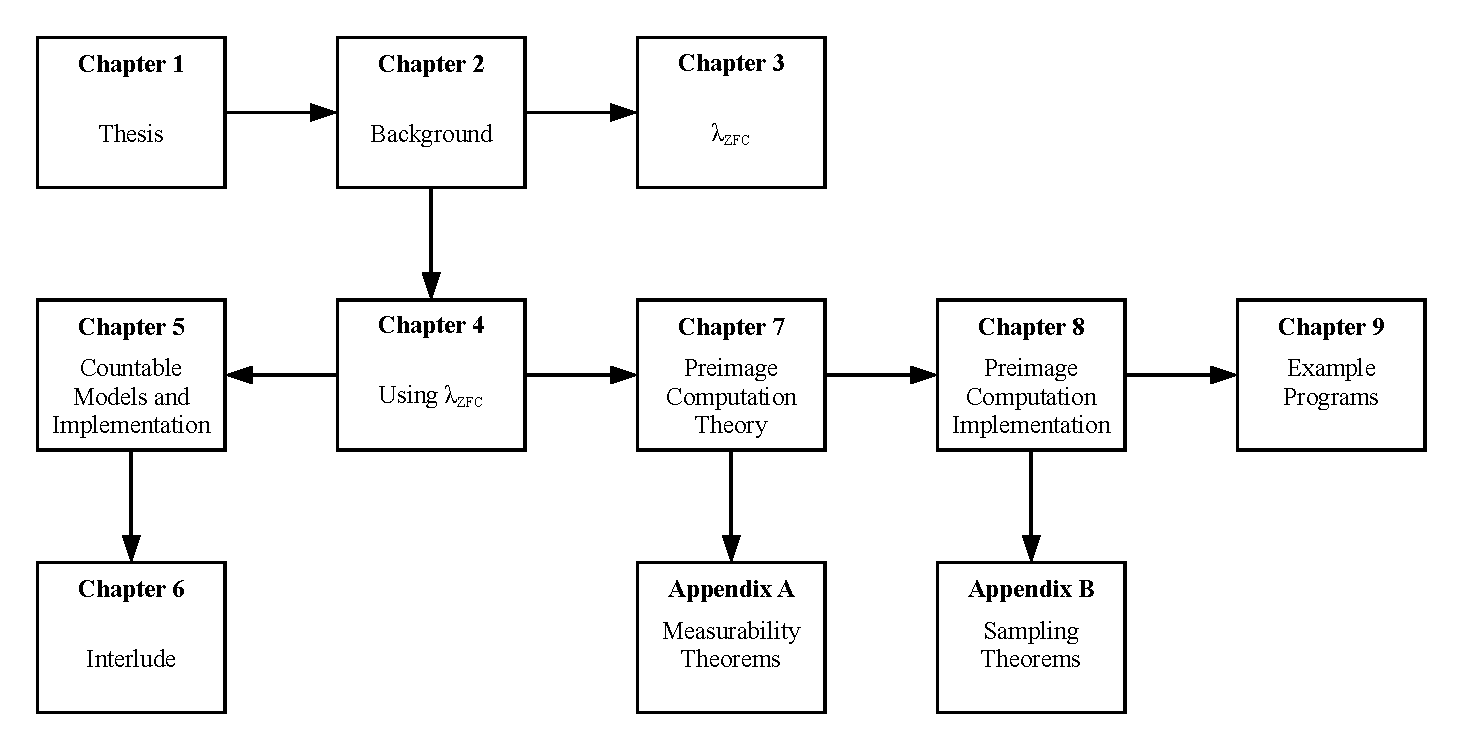
\includegraphics[width=\textwidth]{figures/reading-graph}
\caption[A transition system for reading this dissertation]{A transition system showing possible paths through this dissertation.}
\label{fig:reading-graph}
\end{figure*}

In principle, answers to questions such as ``Which chapters should I read if I am only interested in implementations of probabilistic languages with conditioning and recursion?'' can be answered using a dependency graph.
However, the graph would be a mess of arrows: for example, everything after Chapter~\ref{ch:background} (Background) depends on Chapter~\ref{ch:background}; similarly for Chapter~\ref{ch:using-lambda-zfc} (Using \lzfclang).
\figref{fig:reading-graph} shows an alternative: a transition system on chapters for which following any path (with backtracking permitted) guarantees a reader will not miss out on prerequisites.

Chapter~\ref{ch:background} gives the necessary background in Bayesian practice and functional programming theory, and motivates using measure theory.

The two semantics mentioned in the preceeding section transform programs into $\lambda$-calculus terms.
This target language has three requirements that are unusual for a $\lambda$-calculus: it must be able to represent infinite objects and operations on them, it must have nonterminating programs, and measure-theoretic theorems must apply directly to its terms.
Before this work, such a $\lambda$-calculus did not exist.
Chapter~\ref{ch:lambda-zfc} defines one, \lzfclang, with the precision necessary to carry out proofs with it.

While this precision is necessary for doing the rest of our work and verifying it, such precision is not necessary for understanding it.
Readers who are not verifying our work may therefore skip from Chapter~\ref{ch:background} to Chapter~\ref{ch:using-lambda-zfc}, which gives an overview of \lzfclang and its relationship with contemporary mathematics, gives examples of use, and defines some common terminology and functions.

Chapter~\ref{ch:countable-models} defines a semantics for Bayesian notation restricted to countable probability distributions and finitely many statements.
Chapter~\ref{ch:interlude} explains why its specific way of transforming notation into models does not extend easily to theories with recursion, which motivates a slight change in tactics.

Following the new tactics, Chapter~\ref{ch:preimage1} defines a semantics for a probabilistic language with uncountable distributions, recursion, and arbitrary probabilistic conditions.
Chapter~\ref{ch:preimage2} gives details that should be common to all implementations, and details specific to ours.

Appendix~\ref{ch:measurability} contains proofs of theorems critical to correctness, but whose inclusion in Chapter~\ref{ch:preimage1} would interrupt the narrative flow too much for readers unfamiliar with measure theory.
Appendix~\ref{ch:sampling-algorithm-proofs} is similar, but contains proofs of theorems from Chapter~\ref{ch:preimage2}.
While familiarity with measure theory is helpful while reading these two chapters, it is not strictly necessary: both explain the necessary concepts, and import enough definitions and lemmas from other sources to verify the proofs.



\chapter{Background}

Our work bridges Bayesian practice and functional programming theory using measure-theoretic probability.

In this chapter, we attempt to give enough background to motivate and explain Bayesian practice and functional programming theory.
We only \emph{motivate} measure-theoretic probability here.
Further on, we introduce, explain and use parts as we need them.

It is difficult to find two areas in computer science as different as Bayesian practice and functional programming theory.
In Bayesian practice, we find deeply held belief that unknowns can and should be \emph{quantified} (by probabilities), reasoning by probabilistic inference, willingness to accept many kinds of approximations, and common notation that is---to put it kindly---flexible.
In functional programming theory, we find deeply held belief that unknowns should be \emph{qualified} (usually universally), reasoning by logical inference, little tolerance for unsound approximations even if they converge, and common notation that is---to put it kindly---almost precise enough to feed a compiler.

There is one common trait that makes bridging both areas even conceivable.
While Bayesians model processes and functional programming researchers model languages, both approach their tasks methodically, and both create theories in which every entity they want to reason about is represented explicitly.
If something important is going on behind the scenes---whether a hidden Markov process or mutating the program's store---it is brought to the fore and fully characterized.
In both areas, the extra time and cognitive burden are considered worthwhile payment for reliable artifacts and repeatable results.

It is this trait, explicit representation, that makes it possible to automate Bayesian inference, and again this trait that makes it possible to prove the automation correct.


\section{Bayesian Practice}

From Bayesian practice, the requisite background knowledge includes probability mass functions, probability densities, queries and manipulation rules, Bayesian modeling, and Bayesian inference.
We assume readers know arithmetic, some set theory, functions, and the basic ideas behind integration.

\subsection{Discrete Probability and Joint Distribution Models}

In a probabilistic model of a real-world process, distinguished identifiers called \keyword{random variables} denote random values.
These are regarded as free variables, but with additional information that quantifies the likelihoods of every \emph{combination} of their values, or \keyword{observable outcomes}.
The additional information is completely characterized by a function called a \keyword{joint distribution}.

For example, suppose $X,Y \in \set{h,t}$ are random variables that each represent the outcome of a coin toss.
Further, let the joint distribution $p_{X,Y} : \set{h,t} \times \set{h,t} \to [0,1]$ quantify the likelihood of every possible combination of observable outcomes by defining
\begin{equation}
	p_{X,Y}\ =\ \left[(h,h) \mapsto \frac{1}{4},
		(h,t) \mapsto \frac{1}{4},
		(t,h) \mapsto \frac{1}{6},
		(t,t) \mapsto \frac{1}{3}\right]
\end{equation}
(The subscript ``$X,Y$'' is just part of the function name, and has no special meaning.)
This is a \keyword{probability mass function}: its outputs sum to $1$.

The probability that $X = t$ and $Y = h$ is $p_{X,Y}(t,h) = \frac{1}{6}$.
Another way to write ``the probability that $X = t$ and $Y = h$'' is with a \keyword{probability query}:
\begin{equation}
	\Pspec{X = t \band Y = h}\ =\ p_{X,Y}(t,h)
\end{equation}
A probability query always implicitly refers to some ambient joint distribution.
In general, the result of a probability query $\Pspec{e}$ is the sum of probabilities of observable outcomes for which the proposition $e$ is true.
Conjunctions are often separated by a comma; e.g. $\Pspec{X = x, Y = y}$ means $\Pspec{X = x \band Y = y}$.

Probability queries have manipulation rules.
One is that random variables may be ``summed out'' to consider the probabilities of the values of others independently.
For example, to consider just the probabilities of values of $X$, we may sum out $Y$:
\begin{equation}
	\Pspec{X = x}\ =\ \sum_{y \in \set{h,t}} \Pspec{X = x, Y = y}
\end{equation}
According to this rule, $X$ represents the outcome of a fair coin toss (independent of $Y$):
\begin{equation}
\begin{aligned}
	\Pspec{X = h}&\ =\ \Pspec{X = h, Y = h} + \Pspec{X = h, Y = t}\ =\ \frac{1}{4} + \frac{1}{4}&=\ \frac{1}{2}
\\
	\Pspec{X = t}&\ =\ \Pspec{X = t, Y = h} + \Pspec{X = t, Y = t}\ =\ \frac{1}{6} + \frac{1}{3}&=\ \frac{1}{2}
\end{aligned}
\end{equation}

Another manipulation rule allows fixing the value of one random variable to consider the probabilites of the values of others \emph{dependently}.
For example, if $x$ is fixed and $\Pspec{X = x} > 0$, then the probability that $Y = y$ is
\begin{equation}
	\Pspec{Y = y \given X = x}\ =\ \frac{\Pspec{X = x,Y = y}}{\Pspec{X = x}}
\end{equation}
This \keyword{conditional probability} query is read ``the probability that $Y = y$ given $X = x$.''
Using this rule, we can determine that, if $X$ is known to be $t$, then $Y$ represents a coin toss that is not fair:
\begin{equation}
\begin{aligned}
	\Pspec{Y = h \given X = t}&\ =\ \frac{\Pspec{X = t,Y = h}}{\Pspec{X = t}}\ =\ \frac{\frac{1}{6}}{\frac{1}{2}}&=\ \frac{1}{3}
\\
	\Pspec{Y = t \given X = t}&\ =\ \frac{\Pspec{X = t,Y = t}}{\Pspec{X = t}}\ =\ \frac{\frac{1}{3}}{\frac{1}{2}}&=\ \frac{2}{3}
\end{aligned}
\end{equation}
We could similarly show $\Pspec{Y = h \given X = h} = \frac{1}{2}$ and $\Pspec{Y = t \given X = h} = \frac{1}{2}$, so when $X$ is known to be $h$, $Y$ represents a fair coin toss.

To avoid the condition $\Pspec{X = x} > 0$, the preceeding rule is often written
\begin{equation}
\begin{aligned}
	\Pspec{X = x, Y = y}&\ =\ \Pspec{X = x} \cdot \Pspec{Y = y \given X = x} \\
	&\ =\ \Pspec{Y = y} \cdot \Pspec{X = x \given Y = y}
\end{aligned}
\end{equation}
In this form, it is called the \keyword{chain rule}.

As a function of $x$, $\Pspec{X = x}$ is a probability mass function, but over just $X$ instead of $X$ and $Y$ together.
With any fixed $x$, as a function of $y$, $\Pspec{Y = y \given X = x}$ is also a probability mass function.
Most Bayesian models are constructed by reifying these queries as functions called (respectively) \keyword{distributions} and \keyword{conditional distributions}, and using the chain rule to build a joint distribution.
For the present example,
\begin{equation}
\begin{aligned}
	p_X&\ =\ \left[h \mapsto \frac{1}{2}, t \mapsto \frac{1}{2}\right]
\\
	p_{Y|X}(y \given x)&\ =\
	\begin{cases}
		x = h & \left[h \mapsto \frac{1}{2}, t \mapsto \frac{1}{2}\right](y) \\
		x = t & \left[h \mapsto \frac{1}{3}, t \mapsto \frac{2}{3}\right](y)
	\end{cases}
\\
	p_{X,Y}(x,y)&\ =\ p_X(x) \cdot p_{Y|X}(y \given x)
\end{aligned}
\end{equation}
In the conditional distribution $p_{Y|X}$, the ``$Y|X$'' subscript is simply part of the function name, and in applying it, $(y \given x)$ is just another way to write the arguments $(y,x)$.\footnote{It is common to leave off subscripts such as $Y|X$ and use the form of application to distinguish the different $p$s; e.g. $p(x)$ means $p_X(x)$ and $p(y \given x)$ means $p_{Y|X}(y \given x)$. Doing so is helpful when there are many random variables, and it is usually unambiguous, but the practice often confuses and frustrates newcomers.}
The syntax simply connotes that we expect $\Pspec{Y = y \given X = x}\ =\ p_{Y|X}(y \given x)$.

This model can be more compactly specified by a constructive theory about $X$ and $Y$, which states only the properties that a joint distribution model must satisfy:
\begin{equation}
\begin{aligned}
	X&\ \sim\ \left[h \mapsto \frac{1}{2}, t \mapsto \frac{1}{2}\right]
\\
	Y&\ \sim\ 
	\begin{cases}
		X = h & \left[h \mapsto \frac{1}{2}, t \mapsto \frac{1}{2}\right] \\
		X = t & \left[h \mapsto \frac{1}{3}, t \mapsto \frac{2}{3}\right]
	\end{cases}
\end{aligned}
\end{equation}
Here, $X \sim e$ is read ``$X$ is distributed $e$.''
In this leaner form, it is perhaps easier to understand the process being modeled, which is
\begin{enumerate}
	\item Toss a coin and call its outcome $X$.
	\item If $X = h$, toss a fair coin and call its outcome $Y$.
	\item If $X = t$, toss a biased coin with heads probability $\frac{1}{3}$ and call its outcome $Y$.
\end{enumerate}
It is usually easy to manually translate constructive theories into programs that sample random variable values.

By combining a conditional probability query and the chain rule (or using the chain rule twice), we get \keyword{Bayes' law}: if $\Pspec{Y = y} > 0$, then
\begin{equation}
	\Pspec{X = x \given Y = y}\ =\ \frac{\Pspec{X = x} \cdot \Pspec{Y = y \given X = x}}{\Pspec{Y = y}}
\end{equation}
This is different than $\Pspec{Y = y \given X = x}$.
This time, we are interested in the conditional probability that $X = x$ given we know $Y = y$ for some fixed $y$.

For example, suppose we did not observe $X$, but were allowed to observe $Y = t$.
Given that we know the second coin toss is tails, the probability that $X = t$ is
\begin{equation}
\begin{aligned}
	\Pspec{X = t \given Y = t}&\ =\ \frac{\Pspec{X = t} \cdot \Pspec{Y = t \given X = t}}{\Pspec{Y = t}}
\\
	&\ =\ \frac{\frac{1}{2} \cdot \frac{2}{3}}{\sum_{x \in \set{h,t}} \Pspec{X = x, Y = t}}
\\
	&\ =\ \frac{\frac{1}{2} \cdot \frac{2}{3}}{\frac{1}{4} + \frac{1}{3}}
	\ =\ \frac{\frac{1}{3}}{\frac{7}{12}}
	\ =\ \frac{4}{7}
\end{aligned}
\end{equation}
which is greater than $\Pspec{X = t} = \frac{1}{2}$.
Similarly, $\Pspec{X = h \given Y = t} = \frac{3}{7}$, which is less than $\Pspec{X = h} = \frac{1}{2}$.
Observing the effects of the first coin toss---even random effects---allows us to draw stronger conclusions about the first coin toss.
In this case, we know it is more likely to be tails.

Using Bayes' law to draw probabilistic conclusions about probabilistic processes given observed probabilistic effects is called \keyword{Bayesian inference}.

It is easy for probability newcomers with logical background to think of conditional queries as a fuzzy kind of logical implication.
A short example demonstrates that doing so leads to faulty intuition.
To compute the probability that $Y = t \implies X = t$, we apply logical rules to the query until it is a disjunction of distinct observable outcomes, and add their probabilities:
\begin{equation}
\begin{aligned}
	\Pspec{Y = t \implies X = t}
	&\ =\ \Pspec{\neg (Y = t) \bor X = t}
\\
	&\ =\ \Pspec{Y = h \bor X = t}
\\
	&\ =\ \Pspec{(Y = h \band X = t) \bor (Y = h \band X = h) \bor (Y = t \band X = t)}
\\
	&\ =\ \Pspec{Y = h \band X = t} + \Pspec{Y = h \band X = h} + \Pspec{Y = t \band X = t}
\\
	&\ =\ \frac{1}{6} + \frac{1}{4} + \frac{1}{3} \ =\ \frac{3}{4}
\end{aligned}
\end{equation}
This is clearly not $\Pspec{X = t \given Y = t} = \frac{4}{7}$.
In a similar fashion, $\Pspec{Y = t \implies X = h} = \frac{2}{3}$, which is not $\Pspec{X = h \given Y = t} = \frac{3}{7}$.

In conditioning on $Y = t$, we did not consider any outcomes in which $Y \neq t$: we restricted the possible outcomes to those for which $Y = t$ and renormalized the probabilities of $X = h$ and $X = t$.
On the other hand, in computing the probability that $Y = t \implies X = t$, we had to consider \emph{all} of the outcomes in which $Y \neq t$, and only \emph{one} outcome in which $Y = t$.


\subsection{Probability Densities and Density Models}

Probability mass functions cannot quantify the likelihoods of uncountably many observable outcomes, such as when $X \in \Re$.
In these cases, the distributions, conditional distributions, and joint distributions are specified using \keyword{probability density functions}: functions over outcomes that \emph{integrate} to $1$ instead of sum to $1$.\footnote{For readers familiar with measure theory: we use the word \emph{density} for densities with respect to Lebesgue measure, and \emph{mass} for densities with respect to counting measure. We call all other densities \emph{derivatives}.}

\begin{figure*}[tb]\centering
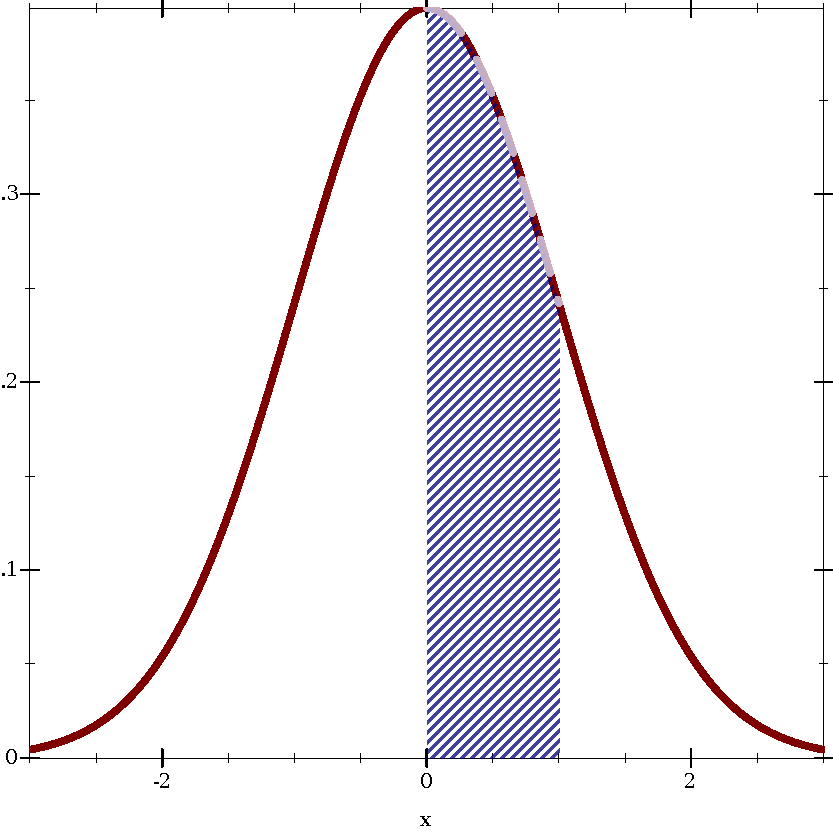
\includegraphics[width=4in]{figures/density-integrate}
\caption[Computing probabilities using the standard normal density function]{Integrating under the standard normal density to compute $\Pspec{X \in (0,1)} \approx 0.34$.}
\label{fig:density-integrate}
\end{figure*}

For example, this probability density function defines the \keyword{standard normal distribution}, or bell curve:
\begin{equation}
	f_N(x)\ =\ \frac{1}{\sqrt{2\pi}} \exp\left(-\frac{x^2}{2}\right)
\end{equation}
If $X$ has a standard normal distribution, then the probability that $X \in (0,1)$ is
\begin{equation}
	\Pspec{X \in (0,1)}\ =\ \int_0^1 f_N(x)\,dx\ \approx\ 0.3413447460685
\end{equation}
Figure~\ref{fig:density-integrate} plots this density and illustrates integrating under it to compute $\Pspec{X \in (0,1)}$.

When probabilities are computed by integrating density functions, sets of outcomes may have positive probability, but every \emph{single} outcome has zero probability.
For any random variable $X \in \Re$, outcome $x \in \Re$, and density function $f_X : \Re \to [0,+\infty)$,
\begin{equation}
	\Pspec{X = x}\ =\ \int_x^x f_X(x)\, dx\ =\ (f_X(x) - 0) \cdot (x - x)\ =\ f_X(x) \cdot 0\ =\ 0
\end{equation}
As a consequence, interval endpoints do not matter; i.e. $\Pspec{X \in [a,b]}\ =\ \Pspec{X \in (a,b)}$.
We discuss other, more difficult consequences further on.

\begin{figure*}[tb]\centering
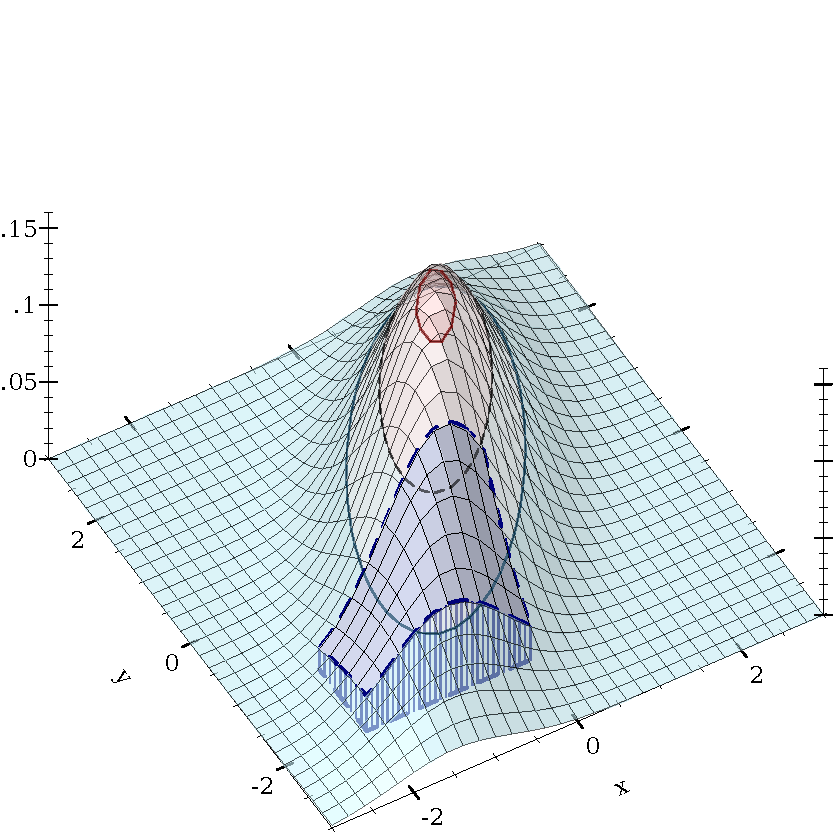
\includegraphics[width=4in]{figures/2d-density-integrate}
\caption[Joint density model plot]{The joint density model $f_{X,Y}$ constructed from the density $f_X$ and the conditional density $f_{Y|X}$. Integrating under $f_{X,Y}$ on the set $(-2,0) \times (-2,-1)$ computes $\Pspec{X \in (-2,0), Y \in (-2,-1)}$.}
\label{fig:joint-density-model}
\end{figure*}

The normal distribution can be extended to a \keyword{distribution family} by parameterizing it on a \emph{mean} $\mu$ and a \emph{standard deviation} $\sigma$:
\begin{equation}
	f_N(x \given \mu,\sigma)\ =\ \frac{1}{\sigma\sqrt{2\pi}} \exp\left(-\frac{(x-\mu)^2}{2\sigma^2}\right)
\end{equation}
(Again, the application syntax $(x \given \mu, \sigma)$ simply means $(x,\mu,\sigma)$.)
Using parameterized distributions, we can define a \keyword{joint density model} of a probabilistic process involving two random variables $X,Y \in \Re$:
\begin{equation}
\begin{aligned}
	f_X(x)&\ =\ f_N(x \given 0,1) \\
	f_{Y|X}(y \given x)&\ =\ f_N(y \given x,1) \\
	f_{X,Y}(x,y)&\ =\ f_X(x) \cdot f_{Y|X}(y \given x)
\end{aligned}
\end{equation}
Integrating under $f_{X,Y}$ computes probability queries:
\begin{equation}
	\Pspec{X \in (a,b), Y \in (c,d)}\ =\ \int_a^b \int_c^d f_{X,Y}(x,y)\,dy\,dx
\end{equation}
Figure~\ref{fig:joint-density-model} illustrates the joint density model $f_{X,Y}$ and computing a probability query.

As with discrete models, density models can be specified by constructive theories:
\begin{equation}
\begin{aligned}
	X&\ \sim\ \mathrm{Normal}(0,1) \\
	Y&\ \sim\ \mathrm{Normal}(X,1)
\end{aligned}
\end{equation}
The probabilistic process being modeled is
\begin{enumerate}
	\item Choose $X$ according to the standard normal distribution.
	\item Choose $Y$ according to the normal distribution with mean $X$, standard deviation $1$.
\end{enumerate}
Again, it is usually easy to manually translate such theories into programs that sample random variable values.

When all single outcomes have zero probability, interpreting theories in terms of expected conditional probability queries is difficult.
(In fact, doing so requires measure theory.)
Fortunately, densities have rules analogous to rules for manipulating probability queries, which allow practitioners to derive joint density models from theories and compute a restricted class of conditional queries.
Instances of the two most important rules are
\begin{equation}
\begin{aligned}
	f_{X}(x)&\ =\ \int_{-\infty}^{+\infty} f_{X,Y}(x,y)\,dy
\\
	f_{X,Y}(x,y)&\ =\ f_{X}(x) \cdot f_{Y|X}(y \given x)\ =\ f_{Y}(y) \cdot f_{X|Y}(x \given y)
\end{aligned}
\end{equation}
The second rule is the \keyword{chain rule for densities}, and it justifies constructing the joint density $f_{X,Y}$ from the density $f_X$ and the conditional density $f_{Y|X}$.

The rules for densities can be used to derive \keyword{Bayes' law for densities}: if $f_Y(y) > 0$, then, starting from the right-hand side of the chain rule,
\begin{displaybreaks}
\begin{align*}
	f_{Y}(y) \cdot f_{X|Y}(x \given y)&\ =\ f_{X}(x) \cdot f_{Y|X}(y \given x)
\\*
	f_{X|Y}(x \given y)&\ =\ \frac{f_{X}(x) \cdot f_{Y|X}(y \given x)}{f_{Y}(y)}
\numberthis\\
	&\ =\ \frac{f_{X}(x) \cdot f_{Y|X}(y \given x)}{\displaystyle\int_{-\infty}^{+\infty} f_{X,Y}(x,y)\,dx}
\\
	&\ =\ \frac{f_{X}(x) \cdot f_{Y|X}(y \given x)}{\displaystyle\int_{-\infty}^{+\infty} f_{X}(x) \cdot f_{Y|X}(y \given x)\,dx}
\end{align*}
\end{displaybreaks}
The last form is conveniently in terms of $f_{X}$ and $f_{Y|X}$, which we have on-hand.

Using Bayes' law for densities, we can draw conclusions about $X$ given knowledge about $Y$.
For example, suppose we want to know the distribution of $X$ given $Y = 2$, as a density.
A quite lengthy derivation finally results in
\begin{equation}
\begin{aligned}
	f_{X|Y}(x \given 2)&\ =\ \frac{f_{X}(x) \cdot f_{Y|X}(2 \given x)}{\displaystyle\int_{-\infty}^{+\infty} f_{X}(x) \cdot f_{Y|X}(2 \given x)\,dx}
\\
	&\ =\ \frac{f_N(x \given 0,1) \cdot f_N(2 \given x,1)}{\displaystyle\int_{-\infty}^{+\infty}
	f_N(x \given 0,1) \cdot f_N(2 \given x,1)\,dx}
\\
	&\,\,\cdots\ 
\\
	&\ =\ f_N(x \given 1, \sqrt{\tfrac{1}{2}})
\end{aligned}
\end{equation}
We can answer conditional probability queries such as ``the probability that $X \in (a,b)$ given $Y = 2$'' by integrating $f_{X|Y}(x \given 2)\ =\ f_N(x \given 1, \sqrt{\tfrac{1}{2}})$:
\begin{equation}
	\Pspec{X \in (a,b) \given Y = 2}\ =\ \int_a^b f_N(x \given 1, \sqrt{\tfrac{1}{2}})\,dx
\end{equation}

\begin{figure*}[tbp]\centering
\subfloat[The original joint density model.]{
\label{fig:bayes-densities:1}
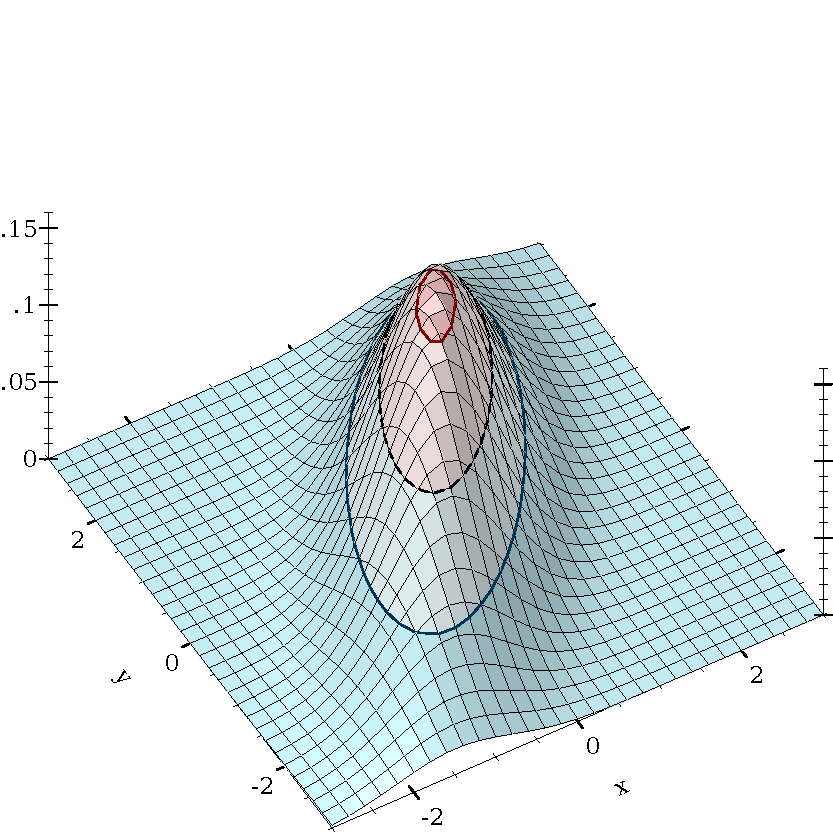
\includegraphics[width=3in]{figures/bayes-densities-1}
}
\tab
\subfloat[Restricting the model to the subset of its domain where $y = 2$. The probability of the subset is zero.]{
\label{fig:bayes-densities:2}
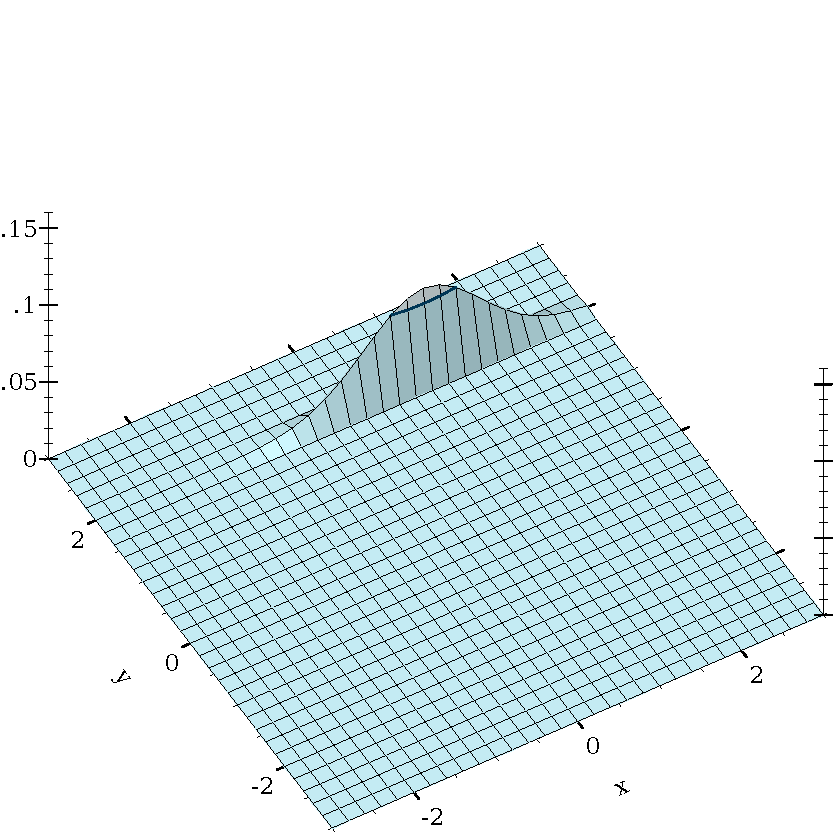
\includegraphics[width=3in]{figures/bayes-densities-2}
}
\vspace{\baselineskip}

\subfloat[Projecting the restricted model onto the $x$ axis results in a density that integrates to a nonzero constant that is less than $1$.]{
\label{fig:bayes-densities:3}
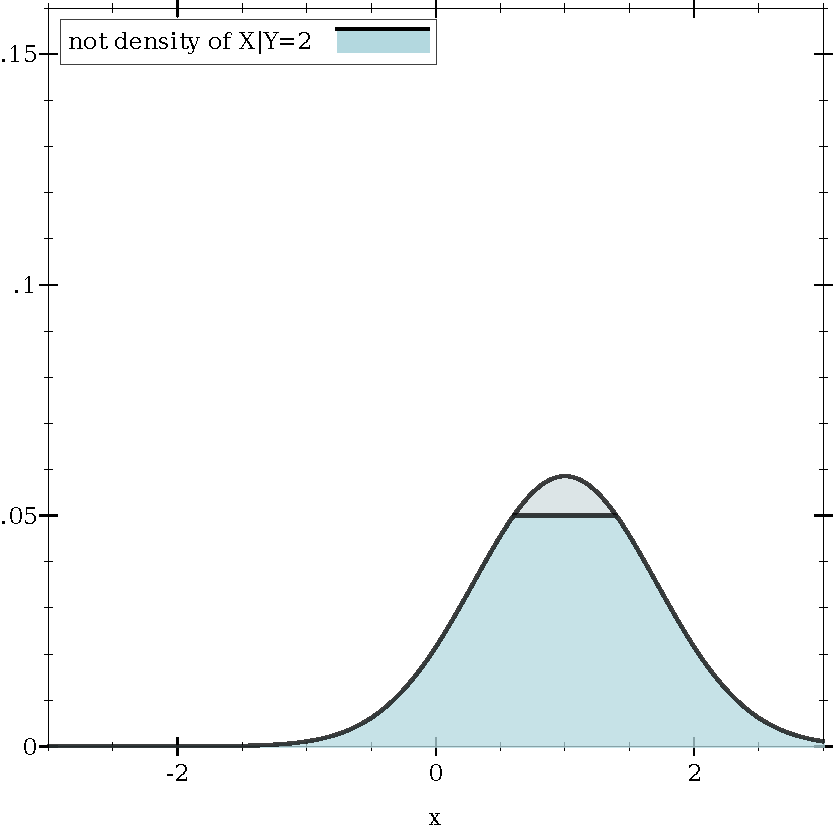
\includegraphics[width=3in]{figures/bayes-densities-3}
}
\tab
\subfloat[Normalizing the restricted, projected model results in a probability density that characterizes the distribution of $X$ given $Y = 2$.]{
\label{fig:bayes-densities:4}
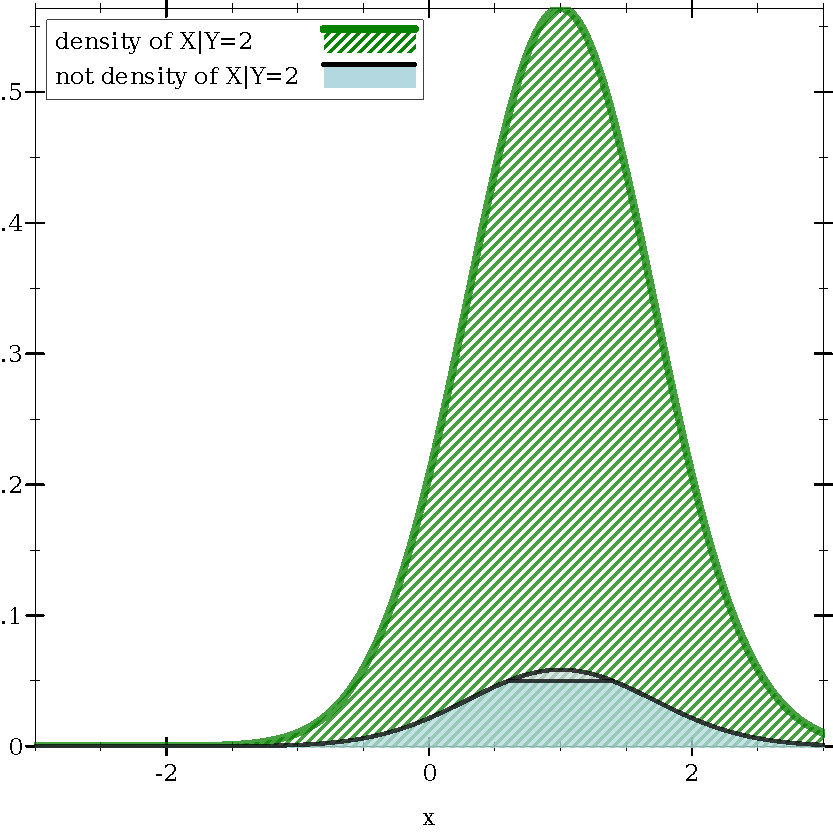
\includegraphics[width=3in]{figures/bayes-densities-4}
}
\caption[Bayes' law for densities, in pictures]{Bayes' law for densities, in pictures.}
\label{fig:bayes-densities}
\end{figure*}

While using Bayes' law for densities is difficult, it is easy to visualize, at least in two dimensions.
We may think of using it as happening in three steps: restrict, project, then renormalize.
\figref{fig:bayes-densities} illustrates them.
First, we restrict the joint density model (\figref{fig:bayes-densities:1}) to the subset of $\Re \times \Re$ where $y = 2$ (\figref{fig:bayes-densities:2}).
Second, because the resulting model integrates to zero and therefore all answers to probability queries using it would be zero, we project it onto the $x$ axis (\figref{fig:bayes-densities:3}), on which it integrates to a positive value.
Third, because the total probability is now less than $1$, we renormalize the restricted, projected model by dividing its output by its area, and obtain a probability density (\figref{fig:bayes-densities:4}).

Using Bayes' law for densities is not only often technically challenging, but in general there are no closed-form solutions.
In such cases, practitioners turn to Monte Carlo integration, or sampling, to answer conditional probability queries.


\subsection{Motivating Measure-Theoretic Models}

It is easy to define a random variable whose distribution cannot be characterized by a density.
Suppose we have a thermometer whose output is not quite correct, but is usually within $1$ degree.
We could model the error with a normal distribution with standard deviation $1$.
If the thermometer cannot show a number greater than $100$ and we want to model that fact, assuming the correct temperature is $99$, we could write a theory about it like this:
\begin{equation}
\begin{aligned}
	T'&\ \sim\ \mathrm{Normal}(99,1) \\
	T&\ =\ \min(T',100)
\end{aligned}
\end{equation}
so that $T$ represents the thermometer's output.
Because $T' \ge 100$ if and only if $T = 100$, $\Pspec{T' \ge 100} = \Pspec{T = 100} > 0$.
But we know that if $T$ has a density, $\Pspec{T = 100} = 0$.

Even though $T$ has no density, it must have a distribution, because $T \in (a,b)$ for any interval $(a,b)$ has a sensible probability, which we can compute by integrating the density of $T'$ up to $100$ and adding $\Pspec{T' \ge 100}$ if the interval happens to contain $100$:
\begin{equation}
	\Pspec{T \in (a,b)}\ =\ \int_{\min(a,100)}^{\min(b,100)} f_N(x \given 99,1)\,dx +
	\begin{cases}
		\Pspec{T' \ge 100} & \text{if $100 \in (a,b)$} \\
		0 & \text{if $100 \notin (a,b)$}
	\end{cases}
\end{equation}
Further, it is easy to write a program that samples $T$ values, and we expect the outputs of programs with probabilistic choice to have well-defined probability distributions.

Another way to define a distribution that cannot be characterized by a density is to restrict a joint density model with a non-axial condition.
For example, with the present theory and density model for $X,Y \in \Re$, suppose we want to answer questions like
\begin{equation}
	\Pspec{X \in (a,b),Y \in (c,d) \given \sqrt{X^2 + Y^2} = 1}
\end{equation}
which restricts the model to a unit circle.
To do so with a density, we need $f_{X,Y|\sqrt{X^2+Y^2}}(x,y \given z)$.
But for any $z$, a joint density for $X,Y$ restricted to $\sqrt{X^2+Y^2} = z$ cannot exist because the area of that circular set is zero.

In the preceeding examples, on a part of the distribution's domain that has length or area $0$ (i.e. the single outcome $100$ or the set $\setb{x \in \Re, y \in \Re}{\sqrt{x^2+x^2} = z}$), the probability of that set is nonzero.
Integrating on such a set can yield only $0$, so the distributions cannot be defined by densities.

There are many more sensible distributions that cannot be defined by densities, such as the distribution of a random variable with outcomes in $\Re \u \Re^2$ or $\Re^\Nat$.
Not only can sets of such outcomes have sensible probabilities, but as in the thermometer example, \emph{it is easy to define random variables with these distributions}.

Measure theory's answer to this shocking lack of densities is to define probability distributions using \keyword{probability measures}, which map \emph{sets to probabilities} instead of \emph{values to instantaneous changes} in probability.
The measure defining $T$'s distribution directly answers queries such as $\Pspec{T \in (a,b)}$.
There is also a measure defined on sets of $\Re \times \Re$ that directly answers queries such as $\Pspec{X \in (a,b),Y \in (c,d) \given \sqrt{X^2 + Y^2} = 1}$.
Probability measures exist on spaces with varying and infinite dimension.

Chapter~\ref{ch:countable-models} introduces measure theory by using it to interpret discrete Bayesian theories mechanically.
Chapter~\ref{ch:preimage1} gives a measure-theoretic interpretation of probabilistic programs, which can encode Bayesian theories that do not have density models.


\begin{comment}
The greatest commonality in the two sides is the attitude with which they approach modeling.
While Bayesian practitioners model processes and functional programming researchers model languages, both approach their tasks methodically, and both create models in which every entity they want to reason about is represented explicitly---sometimes painfully so.
Both sides trust their explicit models to lead to more reliable artifacts and repeatable results than models created by other means.

Therefore, for us, choosing a side to target for publication comes down to determining which side's venues will tolerate the precision necessary to explicitly define our models.
At this stage, in which we almost exclusively model languages, it is clear that we must choose functional programming.
Thus, most of this dissertation assumes readers are functional programming researchers, and tutors them in the necessary Bayesian background.

For readers who are not functional programming researchers, we present this overview of the relevant functional programming theory, and beg their indulgence as we use it to model languages with enough precision to make our artifacts reliable and our results repeatable.

We assume readers know basic computer science theory, including propositional logic, relations, functions, proof by induction, context-free grammars, and nondeterminism.

\end{comment}

\section{Functional Programming Theory}

From functional programming theory, the requisite background knowledge includes the $\lambda$-calculus, big-step operational semantics, denotational semantics, categorical semantics, and abstract interpretation.
We assume readers know basic computer science theory, including propositional logic, relations, functions, proof by induction, context-free grammars, and nondeterminism.

\subsection{$\lambda$-Calculus}

The following grammar defines a set of variable names $X$ and a language $E$ (a set of terms) called the \keyword{pure $\lambda$-calculus}.
\begin{equation}
\begin{aligned}
	e\ ::=&\ x\ |\ e~e\ |\ \fun{x} e \\
	x\ ::=&\ \text{[variable names]}
\end{aligned}
\end{equation}
Terms $\fun{x} e$ are unnamed functions of one argument, terms $x$ refer to function arguments, and terms $e_1~e_2$ apply $e_1$ to $e_2$ (i.e. ``call'' function $e_1$ with argument $e_2$).
For readers unused to the $\lambda$-calculus but familiar with other mathematical languages, perhaps the most difficult thing to get used to is that juxtaposition means application instead of multiplication.

As in most mathematical languages, parentheses are optional.
Lambda terms greedily enclose their bodies in implicit parentheses, so $\fun{x}\fun{y} e$ (with some assumed-meaningful function body $e$) is the same term as $\fun{x}(\fun{y} e)$: a function that receives an $x$ and returns a function of $y$ in which $x$ is available.
Application is left-associative, so $e_1~e_2~e_3$ is the same term as $(e_1~e_2)~e_3$.
Here, $e_1~e_2$ returns a function, which is applied to $e_3$.

This duality makes it easy to write two-argument functions using nested lambdas, and apply them using sequences of arguments.
For example, $(\fun{x} \fun{y} e)~e_x~e_y$ defines a function of two arguments and applies it to $e_x$ and $e_y$.

Like its younger brother the Turing machine, the pure $\lambda$-calculus is a universal model of computation.
Also like the Turing machine, it would be quite painful to program with it.
Unlike the Turing machine, it is easy to get something practical with a few extensions such as pairs and numbers, and a few primitive functions to operate on them.

In most programming languages, implementation details define the meaning of function application.
It typically involves a jump from one machine address to another, and if the function returns, a jump back.
However, in the pure $\lambda$-calculus and its extensions, there are no jumps or machine addresses.
Function application is defined entirely in terms of substitution, as in algebra.
For example, suppose  $\mathit{hypot}$ is a term in a $\lambda$-calculus extended with real numbers, defined by
\begin{equation}
	\mathit{hypot}\ =\ \fun{x}\fun{y} \sqrt{x^2 + y^2}
\end{equation}
Applying $\mathit{hypot}$ eliminates lambdas by substituting their formal arguments with the supplied actual arguments:
\begin{equation}
\begin{aligned}
	\mathit{hypot}~3~4
		&\ =\ \left(\fun{x}\fun{y} \sqrt{x^2 + y^2}\right)~3~4 \\
		&\ =\ \left(\left(\fun{x}\left(\fun{y} \sqrt{x^2 + y^2}\right)\right)~3\right)~4 \\
		&\ \equiv\ \left(\fun{y} \sqrt{3^2 + y^2}\right)~4 \\
		&\ \equiv\ \sqrt{3^2 + 4^2} \\
\end{aligned}
\label{eqn:lambda-calculus-reduce1}
\end{equation}
The two equivalences at the end of~\eqref{eqn:lambda-calculus-reduce1} are called \keyword{$\beta$-reductions}, or just \keyword{reductions}.
We would expect $\sqrt{3^2 + 4^2}$ to further reduce to $5$.

Computer implementations of an extended $\lambda$-calculus, such as the programming language Racket, necessarily use jumps and machine addresses to implement function application.
However, the meanings of their programs are defined mathematically as the results of carrying out reductions.
It is therefore possible to reason about programs algebraically and inductively, without having to consider complicating machine details.

It is sometimes convenient to define a $\lambda$-calculus whose variables refer to function arguments by \emph{number} instead of by \emph{name}.
Such numeric references are called \keyword{De Bruijn}\footnote{Typically pronounced ``deh brOIN,'' and named after Dutch mathematician Nicolaas de Bruijn.} \keyword{indexes}.
One form of the pure $\lambda$-calculus with De Bruijn indexes is
\begin{equation}
\begin{aligned}
	e\ ::=&\ \mathsf{env}~n\ |\ e~e\ |\ \lfun e \\
	n\ ::=&\ 0\ |\ 1\ |\ 2\ |\ \cdots
\end{aligned}
\end{equation}
where a ``variable'' term $\mathsf{env}~0$ refers to the innermost lambda's argument.

Suppose we define $\mathit{hypot}$ as a term in a $\lambda$-calculus with De Bruijn indexes, extended with real numbers:
\begin{equation}
	\mathit{hypot}\ =\ \lfun\lfun\sqrt{(\mathsf{env}~1)^2 + (\mathsf{env}~0)^2}
\end{equation}
Here, $\mathsf{env}~1$ (which was previously $x$) refers to the outer lambda's argument and $\mathsf{env}~0$ refers to the inner lambda's argument.
Reducing an application of $\mathit{hypot}$ proceeds this way:
\begin{equation}
\begin{aligned}
	\mathit{hypot}~3~4
		&\ =\ \left(\lfun\lfun \sqrt{(\mathsf{env}~1)^2 + (\mathsf{env}~0)^2}\right)~3~4 \\
		&\ \equiv\ \left(\lfun \sqrt{3^2 + (\mathsf{env}~0)^2}\right)~4 \\
		&\ \equiv\ \sqrt{3^2 + 4^2} \\
\end{aligned}
\label{eqn:lambda-calculus-reduce2}
\end{equation}

So far, we have been taking a certain evaluation order for granted when computing reductions.
To highlight an ambiguity, consider this lambda term, which returns $0$ given any argument:
\begin{equation}
	\mathit{zero}\ =\ \fun{x} 0
\end{equation}
Suppose $1~{/}~0$ does not reduce to any value, as in algebra.
Should $\mathit{zero}~(1~{/}~0)$ reduce to $0$, or likewise not reduce?
In other words, should we accept this reduction:
\begin{equation}
\begin{aligned}
	\mathit{zero}~(1~{/}~0)
	&\ =\ (\fun{x} 0)~(1~{/}~0)
\\
	&\ \equiv\ 0
\end{aligned}
\end{equation}
or should we require function arguments to reduce before substituting them?
Always reducing function arguments first is \keyword{call-by-value} reduction, and substituting without reducing arguments is \keyword{call-by-name}.
Both policies have their place, but we mostly use call-by-value reduction, in which $\mathit{zero}~(1~{/}~0)$ does not reduce.

%Plotkin, Scott, Steele and many others following: work on correspondence of $\lambda$-calculus reduction with machine execution makes it possible to define an implementable theory for a programming language

\subsection{Big-Step Operational Semantics}

Instead of describing evaluation order using English phrases with scattered mathematical terms, we could instead give our $\lambda$-calculus a \keyword{semantics}: a precise mathematical definition of the meaning of its terms.
To specify evaluation order and other operational aspects specifically, we would typically give it an \keyword{operational semantics}.

An operational semantics is defined by a \keyword{reduction relation}, which relates program terms to other program terms.
There are two main kinds of operational semantics:
\begin{itemize}
	\item \keyword{Small-step}, specified by a subset of $E \times E$, where $E$ is the set of program terms.
	\item \keyword{Big-step}, specified by a subset of $E \times V$, where $E$ is the set of program terms and $V \subseteq E$ is the set of irreducible program values (e.g. the number $4$, the pair $\pair{10,23}$).
\end{itemize}
For example, suppose we have a lambda term
\begin{equation}
	\mathit{inc}\ =\ \fun{x} x + 1
\end{equation}
A small-step semantics would typically ``stop'' after a function application.
If ``$\Rightarrow$'' is a small-step reduction relation, then $(\mathit{inc}~4) \Rightarrow (4 + 1)$ should be true, and also $(4 + 1) \Rightarrow 5$, so we can conclude $\mathit{inc}~4$ reduces to $5$ in two \keyword{small steps}.
On the other hand, a big-step semantics cannot ``stop'' after most function applications.
If ``$\dto$'' is a big-step reduction relation, then we cannot expect $(\mathit{inc}~4) \dto (4 + 1)$ because by any reasonable definition, the term $4 + 1$ is an \emph{expression} but not a \emph{value}.
We should expect, however, that $(\mathit{inc}~4) \dto 5$ is true; i.e. $\mathit{inc}$ reduces to $5$ in one \keyword{big step}.

As with call-by-name and call-by-value, small-step and big-step semantics both have their place.
However, as Chapter~\ref{ch:lambda-zfc} contains the only operational semantics in this disseration and it is a big-step semantics, we concentrate on big-step in this overview.

\begin{figure*}[tb]\centering
\subfloat[A grammar to define sets $E$ and $V$]{
\label{fig:add-language:grammar}
\begin{minipage}[b]{2.5in}
\begin{equation*}
\begin{aligned}
	&e\ ::=\ v\ |\ \mathsf{add}~e~e \\
	&v\ ::=\ 0\ |\ 1\ |\ 2\ |\ \cdots
\end{aligned}
\end{equation*}
\hrule
\end{minipage}
}
\tab\tab
\subfloat[Reduction rules to define $\dto \subseteq E \times V$]{
\label{fig:add-language:reduction}
\begin{minipage}[b]{3in}
\begin{equation*}
\begin{aligned}
	\dfrac{}{v \dto v}
	\ \text{(val)}
	\jand\jand
	\dfrac{e_1 \dto v_1 \jand e_2 \dto v_2}{(\mathsf{add}~e_1~e_2) \dto (v_1 + v_2)}
	\ \text{(add)}
\end{aligned}
\end{equation*}
\hrule
\end{minipage}
}
\caption[Big-step operational semantics example]{A big-step operational semantics for a simple addition language.}
\label{fig:add-language}
\end{figure*}

\figref{fig:add-language} defines a language and its semantics by giving a grammar and a big-step reduction relation ``$\dto$''.
The language is even simpler than the pure $\lambda$-calculus: its terms simply represent adding concrete numbers.
The relation ``$\dto$'' is defined by \keyword{reduction rules} in the form
\begin{equation}
	\dfrac{\mathit{premise}_1 \jand \mathit{premise}_2 \jand \cdots}{\mathit{conclusion}} \jand \text{(name)}
\end{equation}
Grammar nonterminals are implicitly universally quantified, premises are implicitly conjuncted, and the rule is interpreted as an implication.
For example, the (add) rule in \figref{fig:add-language:reduction} means ``for all $e_1,e_2 \in E$ and $v_1,v_2 \in V$, if $e_1$ reduces to $v_1$ and $e_2$ reduces to $v_2$, then $\mathsf{add}~e_1~e_2$ reduces to $v_1 + v_2$.''
The (val) rule means ``for all $v \in V$, $v$ reduces to $v$'' or equivalently, ``for all $v \in V$, $\mathit{true}$ implies $v$ reduces to $v$.''

The reduction relation ``$\dto$'' is defined as the \emph{smallest} subset of $E \times V$ for which the reduction rules hold.
Defining it as the smallest subset precludes unintended conclusions such as $4 \dto 5$, which are not otherwise precluded by interpreting the rules as implications.
Equivalently, it restricts ``$\dto$'' to conclusions that are provable from the reduction rules.

Reduction rules can be used directly to build \keyword{derivation trees}, which represent both computation steps and proofs of conclusions.
For example, suppose we want to use the reduction rules in \figref{fig:add-language:reduction} to compute the value of $\mathsf{add}~(\mathsf{add}~4~5)~90$.
We start by writing it as a conclusion without premises:
\begin{equation}
	\dfrac{}{(\mathsf{add}~(\mathsf{add}~4~5)~90) \dto v_1}
\label{eqn:add-to-99-start}
\end{equation}
There is only one rule (add) with a matching conclusion, so we add its premises, renaming variables as appropriate:
\begin{equation}
	\dfrac{\dfrac{}{(\mathsf{add}~4~5) \dto v_2} \jand \dfrac{}{90 \dto v_3}}{(\mathsf{add}~(\mathsf{add}~4~5)~90) \dto v_1}
\end{equation}
There is only one rule (val) matching the conclusion $90 \dto v_3$, and it has no premises.
We thus only add premises for the (add) rule matching $(\mathsf{add}~4~5)$:
\begin{equation}
	\dfrac{\dfrac{\dfrac{}{4 \dto v_4} \jand \dfrac{}{5 \dto v_5}}{(\mathsf{add}~4~5) \dto v_2} \jand \dfrac{}{90 \dto v_3}}{(\mathsf{add}~(\mathsf{add}~4~5)~90) \dto v_1}
\end{equation}
It is easy to find values of $v_3$, $v_4$ and $v_5$ that make the leaf premises true, so we substitute them and recursively fill in the conclusions:
\begin{equation}
	\dfrac{\dfrac{\dfrac{}{4 \dto 4} \jand \dfrac{}{5 \dto 5}}{(\mathsf{add}~4~5) \dto v_2} \jand \dfrac{}{90 \dto v_3}}{(\mathsf{add}~(\mathsf{add}~4~5)~90) \dto v_1}
	\Longrightarrow
	\dfrac{\dfrac{\dfrac{}{4 \dto 4} \jand \dfrac{}{5 \dto 5}}{(\mathsf{add}~4~5) \dto 9} \jand \dfrac{}{90 \dto 90}}{(\mathsf{add}~(\mathsf{add}~4~5)~90) \dto v_1}
	\Longrightarrow
	\dfrac{\dfrac{\dfrac{}{4 \dto 4} \jand \dfrac{}{5 \dto 5}}{(\mathsf{add}~4~5) \dto 9} \jand \dfrac{}{90 \dto 90}}{(\mathsf{add}~(\mathsf{add}~4~5)~90) \dto 99}
\label{eqn:add-to-99-conclusion}
\end{equation}
Thus, the rightmost derivation tree in~\eqref{eqn:add-to-99-conclusion} is a proof that $(\mathsf{add}~(\mathsf{add}~4~5)~90) \dto 99$.

In most cases, reduction relations can be mathematically constructed by iterating a function that uses the reduction rules to add more conclusions given known premises.
A fixpoint is reachable in countably many iterations, and as a consequence, derivation trees are always finite.
On the other hand, Chapter~\ref{ch:lambda-zfc} defines a $\lambda$-calculus in which the iterating function must be applied uncountably many times to reach a fixpoint, and as a consequence, its derivation trees may be infinite.
Despite this minor difference in size, the basic principles behind the reduction relation's construction and use are the same.

If a big-step reduction relation ``$\dto$'' relates each left-hand side term to exactly one right-hand side term, it is a total function, or $\dto : E \to V$.
If it relates each left-hand side term to \emph{at most} one right-hand side term, it is a partial function, or $\dto : E \pto V$.
In either case, if its derivation trees are finite, it can be implemented as a recursive function.

\begin{figure*}[tb]\centering
\begin{schemedisplay}
(define value? exact-nonnegative-integer?)
(struct add (e1 e2))
<blank-line>
(define (interp e)
  (match e
    [(? value? v)  v]
    [(add e1 e2)  (define v1 (interp e1))
                  (define v2 (interp e2))
                  (+ v1 v2)]))
\end{schemedisplay}
\bottomhrule
\caption[Implementation of the big-step semantics]{Racket implementation of the semantics defined in \figref{fig:add-language}.}
\label{fig:add-language-impl}
\end{figure*}

\figref{fig:add-language-impl} gives a Racket implementation of ``$\dto$'' in \figref{fig:add-language:reduction}.
(We say Racket is the implementation's \keyword{host language}.)
The implementation defines a structure type \scheme{add} to model $\mathsf{add}$ expressions, and uses Racket's built-in big integers to model $V$.
Computation recursively interprets expressions, and proceeds similarly to the derivation tree construction in~\eqref{eqn:add-to-99-start} through~\eqref{eqn:add-to-99-conclusion}.
As an example of use, at DrRacket's Read-Eval-Print Loop (REPL), we get
\begin{center}
\singlespacing
\begin{schemedisplay}
> (interp (add (add 4 5) 90))
99
\end{schemedisplay}
\end{center}
as expected.

\begin{figure*}[tb]\centering
\subfloat[A grammar to define sets $E$ and $V$]{
\label{fig:add-choose-language:grammar}
\begin{varwidth}[b]{2.4in}
\begin{equation*}
\begin{aligned}
	&e\ ::=\ v\ |\ \mathsf{add}~e~e\ |\ \mathsf{choose}~e~e \\
	&v\ ::=\ 0\ |\ 1\ |\ 2\ |\ \cdots
\end{aligned}
\end{equation*}
\hrule
\end{varwidth}
}
\tab
\subfloat[Reduction rules to define $\dto \subseteq E \times V$]{
\label{fig:add-choose-language:reduction}
\begin{varwidth}[b]{3.7in}
\begin{equation*}
	\dfrac{}{v \dto v}
	\ \text{(val)}
	\jand\jand
	\dfrac{e_1 \dto v_1 \jand e_2 \dto v_2}{(\mathsf{add}~e_1~e_2) \dto (v_1 + v_2)}
	\ \text{(add)}
\end{equation*}
\begin{equation*}
	\dfrac{e_1 \dto v_1}{(\mathsf{choose}~e_1~e_2) \dto v_1}
	\ \text{(left)}
	\jand
	\dfrac{e_2 \dto v_2}{(\mathsf{choose}~e_1~e_2) \dto v_2}
	\ \text{(right)}
	\\[6pt]
\end{equation*}
\hrule
\end{varwidth}
}
\caption[Big-step operational semantics with nondeterminism]{Big-step operational semantics for a language with nondeterministic choice.}
\label{fig:add-choose-language}
\end{figure*}

\figref{fig:add-choose-language} extends the present example language with nondeterministic choice, which results in a reduction relation that is \emph{not} a function.
The culprits are the new rules (left) and (right), which can both match the same conclusion.
For example, suppose we want to use the reduction rules in \figref{fig:add-choose-language:reduction} to compute the value of $\mathsf{add}~(\mathsf{choose}~4~5)~90$.
We start as before, by writing it as a conclusion without premises:
\begin{equation}
	\dfrac{}{(\mathsf{add}~(\mathsf{choose}~4~5)~90) \dto v_1}
\end{equation}
We match the conclusion to the (add) rule and add its premises:
\begin{equation}
	\dfrac{
		\dfrac{}{(\mathsf{choose}~4~5) \dto v_2}
		\jand
		\dfrac{}{90 \dto v_3}
	}{(\mathsf{add}~(\mathsf{choose}~4~5)~90) \dto v_1}
\end{equation}
Again, there is only one rule (val) matching the conclusion $90 \dto v_3$, and it has no premises.
For the conclusion $(\mathsf{choose}~4~5) \dto v_2$, however, we may choose either (left) or (right), leading to two different derivation trees:
\begin{equation}
	\dfrac{
		\dfrac{
			\dfrac{}{4 \dto v_4}
		}{(\mathsf{choose}~4~5) \dto v_2}
		\jand
		\dfrac{}{90 \dto v_3}
	}{(\mathsf{add}~(\mathsf{choose}~4~5)~90) \dto v_1}
	\jand
	\jand
	\dfrac{
		\dfrac{
			\dfrac{}{5 \dto v_5}
		}{(\mathsf{choose}~4~5) \dto v_2}
		\jand
		\dfrac{}{90 \dto v_3}
	}{(\mathsf{add}~(\mathsf{choose}~4~5)~90) \dto v_1}
\end{equation}
After replacing $v_3$, $v_4$ and $v_5$ with the only values that make the leaf premises true and recursively filling in the conclusions, we would find that both $(\mathsf{add}~(\mathsf{choose}~4~5)~90) \dto 94$ and $(\mathsf{add}~(\mathsf{choose}~4~5)~90) \dto 95$ are true, and would have derivation trees to prove these facts.

An implementation of a nondeterministic semantics would be correct if, for every interpretation of a term $e$ that produced value $v$, $e \dto v$ were a valid conclusion.
For $\mathsf{choose}~4~5$, for example, a correct implementation may always choose $4$, always choose $5$, choose randomly, choose the number that gives the best or worst outcome according to some objective function, or always choose $4$ on weekends or during the fall equinox.
Its choice is simply not modeled by the semantics.

Suppose we wanted to compute results for every possible combination of nondeterministic choices.
We could define a big-step relation $\dto : E \to \powerset~V$, which returns (when used as a function) a set of values, and implement an interpreter for it.
However, we are saving that example for the next section.


\subsection{Denotational Semantics}

A \keyword{denotational semantics} is defined by a deterministic \keyword{semantic function} from language terms to values \emph{in another language}.
The other language is called the \keyword{metalanguage} or \keyword{target language}, and is often an axiomatic logic such as first-order set theory (i.e. ordinary mathematics).

\newsavebox{\compileonebox}

\begin{lrbox}{\compileonebox}
\begin{varwidth}[b]{3.3in}
\singlespacing\centering
\begin{schemedisplay}
(define-syntax compile
  (syntax-rules (add)
    [(_ (add e1 e2))  (+ (compile e1)
                         (compile e2))]
    [(_ v)  v]))
\end{schemedisplay}
\hrule
\end{varwidth}
\end{lrbox}

\begin{figure*}[tb]\centering
\subfloat[A semantic function for the addition language]{
\label{fig:add-denotational:semantic-function}
\begin{varwidth}[b]{2.0in}
\begin{equation*}
\meaningof{\cdot} : E \to \Nat
\\[6pt]
\end{equation*}
\begin{equation*}
\begin{aligned}
	\meaningof{v}&\ =\ v \\
	\meaningof{\mathsf{add}~e_1~e_2}&\ =\ \meaningof{e_1} + \meaningof{e_2} \\
\end{aligned}
\end{equation*}
\hrule
\end{varwidth}
}
\tab\tab
\subfloat[An implementation of the semantic function as a syntax transformer]{
\label{fig:add-denotational:implementation}
\usebox{\compileonebox}
}
\caption[Denotational semantics and implementation]{A denotational semantics and its implementation.}
\label{fig:add-denotational}
\end{figure*}

\figref{fig:add-denotational:semantic-function} defines a denotational semantics for the addition language without $\mathsf{choose}$ by defining a semantic function $\meaningof{\cdot} : E \to \Nat$.
The double square brackets are simply a different application syntax: they connote nothing mathematically, but serve as a visual cue to read applications of the semantic function as ``the meaning of'' or ``the denotation of.''
For example, the meaning of $\mathsf{add}~(\mathsf{add}~4~5)~90$ is
\begin{equation}
\begin{aligned}
	\meaningof{\mathsf{add}~(\mathsf{add}~4~5)~90}
	&\ =\ \meaningof{\mathsf{add}~4~5} + \meaningof{90}
\\
	&\ =\ (\meaningof{4} + \meaningof{5}) + \meaningof{90}
\\
	&\ =\ (4 + 5) + 90
\\
	&\ =\ 99
\end{aligned}
\end{equation}
The semantic function is \keyword{compositional}: it gives meaning to terms \emph{by combining the meanings of their direct subterms}.
Compositionality allows most proofs of program properties to be done by structural induction, as we will demonstrate shortly.

When the results of applying $\meaningof{\cdot}$ are computable, because it is compositional, it is often easy to implement it as local syntax transformation or compilation.
\figref{fig:add-denotational:implementation} shows a Racket implementation of $\meaningof{\cdot}$ as a transformation from meaningless parenthetical syntax (an \scheme{add} function does not exist) to runnable Racket syntax.
The syntax transformer is barely more than a transcription of the semantic function's definition, with a little extra code to signal to Racket that it is to be applied to the syntax of expressions before compiling or evaluating them (i.e. \scheme{define-syntax} instead of \scheme{define}) and to identify the symbol \scheme{add} as a terminal symbol.

The results of compilation seem to be equivalent to the results of interpretation:
\begin{center}
\singlespacing
\begin{schemedisplay}
> (compile (add (add 4 5) 90))
99
\end{schemedisplay}
\end{center}
but the REPL does not show transformed syntax.
Fortunately, \scheme{expand-syntax} can show it:
\begin{center}
\singlespacing
\begin{schemedisplay}
> (expand-syntax #'(add (add 4 5) 90))
#'(+ (+ 4 5) 90))
\end{schemedisplay}
\end{center}

\newsavebox{\compiletwobox}

\begin{lrbox}{\compiletwobox}
\begin{varwidth}[b]{3.5in}
\singlespacing
\centering
\begin{schemedisplay}
(define-syntax compile
  (syntax-rules (add choose)
    [(_ (add e1 e2))
     (for*/set ([v1 (in-set (compile e1))]
                [v2 (in-set (compile e2))])
       (+ v1 v2))]
    [(_ (choose e1 e2))
     (set-union (compile e1) (compile e2))]
    [(_ v)
     (set v)]))
\end{schemedisplay}
\hrule
\end{varwidth}
\end{lrbox}

\begin{figure*}[tb]\centering
\begin{varwidth}[b]{\textwidth}
\begin{equation*}
\begin{aligned}[t]
	\meaningof{\cdot} &: E \to \powerset~\Nat
\\[6pt]
	\meaningof{v}&\ =\ \set{v}
\\
	\meaningof{\mathsf{add}~e_1~e_2}&\ =\ \setb{v_1 + v_2}{v_1 \in \meaningof{e_1}, v_2 \in \meaningof{e_2}}
\\
	\meaningof{\mathsf{choose}~e_1~e_2}&\ =\ \meaningof{e_1} \u \meaningof{e_2} \\
\end{aligned}
\end{equation*}
\end{varwidth}
\bottomhrule
\caption[Denotational semantics with nondeterminism]{A denotational semantics for the addition language with nondeterministic choice.}
\label{fig:add-choose-denotational}
\end{figure*}

\figref{fig:add-choose-denotational} defines a compositional function $\meaningof{\cdot} : E \to \powerset~\Nat$, which transforms the addition language with nondeterministic choice into sets of natural numbers.
For example, the meaning of $4$ is $\set{4}$, the meaning of $\mathsf{choose}~4~5$ is $\set{4} \u \set{5} = \set{4,5}$, and the meaning of $\mathsf{add}~(\mathsf{choose}~4~5)~90$ is
\begin{equation}
\begin{aligned}
	\meaningof{\mathsf{add}~(\mathsf{choose}~4~5)~90}
	&\ =\ \setb{v_1 + v_2}{v_1 \in \meaningof{\mathsf{choose}~4~5}, v_2 \in \meaningof{90}}
\\
	&\ =\ \setb{v_1 + v_2}{v_1 \in (\meaningof{4} \u \meaningof{5}), v_2 \in \meaningof{90}} 
\\
	&\ =\ \setb{v_1 + v_2}{v_1 \in (\set{4} \u \set{5}), v_2 \in \set{90}}
\\
	&\ =\ \setb{v_1 + v_2}{v_1 \in \set{4,5}, v_2 \in \set{90}}
\\
	&\ =\ \set{4+90,5+90}
\\
	&\ =\ \set{94,95}
\end{aligned}
\end{equation}
We know that under ``$\dto$,'' $\mathsf{add}~(\mathsf{choose}~4~5)~90$ reduces to both $94$ and $95$, so it appears $\meaningof{\cdot}$ is correct.
It would be nice to know whether it is \emph{always} correct.
The following theorem states correctness precisely in terms of ``$\dto$,'' and critically uses $\meaningof{\cdot}$'s compositionality in a proof by induction on the structure of $e$.

\begin{theorem}[correctness]
For all $v \in V$ and $e \in E$, $v \in \meaningof{e} \iff e \dto v$.
\end{theorem}
\begin{proof}
Let $v \in V$ and $e \in E$.
The proof is by induction on the structure of $e$.

Base case $e \in V$.
If $e = v$, then $v \in \meaningof{e} = \set{e} = \set{v}$ by definition of $\meaningof{\cdot}$, and $e \dto v$ by the (val) rule.
Similarly, if $e \neq v$, then $v \not\in \meaningof{e}$, and not $e \dto v$.

Inductive case $e = \mathsf{add}~e_1~e_2$ for some $e_1 \in E$ and $e_2 \in E$.

Suppose $v \in \meaningof{\mathsf{add}~e_1~e_2}$.
By definition of $\meaningof{\cdot}$, there exist $v_1 \in \meaningof{e_1}$, $v_2 \in \meaningof{e_2}$ such that $v = v_1 + v_2$.
By the inductive hypothesis, $e_1 \dto v_1$ and $e_2 \dto v_2$.
By the (add) rule, $(\mathsf{add}~e_1~e_2) \dto v$.

Conversely, if $(\mathsf{add}~e_1~e_2) \dto v$,
by (add), there exist $v_1,v_2$ such that $e_1 \dto v_1$, $e_2 \dto v_2$ and $v = v_1 + v_2$.
By hypothesis, $v_1 \in \meaningof{e_1}$ and $v_2 \in \meaningof{e_2}$.
By definition of $\meaningof{\cdot}$, $v \in \meaningof{\mathsf{add}~e_1~e_2}$.

Proof of the inductive case $e = \mathsf{choose}~e_1~e_2$ is similar to the preceeding, though each ``${\Longleftrightarrow}$'' direction has in inner case for nondeterministic choice.
\end{proof}

Now that we know $\meaningof{\cdot}$ is correct, we can regard any implementation of it as an implementation of ``$\dto$''  as well.
In general, it is easy to transfer theorems about ``$\dto$'' to a correct $\meaningof{\cdot}$, and vice-versa.

What if we wanted to represent nondeterministic choices using lists instead of sets, or model a different computational effect, such as mutation or probabilitistic choice?
We could define a different semantic function for each model, but there is a more elegant way.


\subsection{Categorical Semantics}

When computer scientists from any area want to extend a fixed process without having to repeat themselves more than necessary, they \keyword{abstract}: they decouple the desired varying part from the fixed process, and parameterize the previously fixed process on the varying part.
This characterizes modular, object-oriented, functional, and even semantic abstraction.

To abstract a denotational semantics, we parameterize its semantic function on the meaning it produces.
The parameter takes the form of a \keyword{category}.\footnote{The word ``category'' comes from category theory, an alternative axiomatization of mathematics. Fortunately, little knowledge of category theory is necesary to define or understand categorical semantics.}
In semantics, the category is comprised of a collection of objects called \keyword{computations} (i.e. possible program meanings) and operations on them called \keyword{combinators}.

The appropriate category for the addition language with $\mathsf{choose}$ contains sets of numbers as computations, or $\powerset~\Nat$, and operations on them.
While there are many possible collections of combinators, one kind of collection that functional programmers and theorists have found very useful are \keyword{monads}.\footnote{Strictly speaking, in category theory, they are \emph{strong} monads.}
The \keyword{set monad} operates on set-valued computations and is defined by these two combinators:
\begin{equation}
\begin{aligned}
	\mathit{return_{set}}~v&\ =\ \set{v} \\
	\mathit{bind_{set}}~A~f&\ =\ \bigcup_{v \in A} f~v
\end{aligned}
\end{equation}
Evidently, from a semantic function $\meaningof{\cdot}_a$ parameterized on a monad $a$ we should expect $\meaningof{v}_\mathit{set} = \mathit{return_{set}}~v \equiv \set{v}$.
How to use $\mathit{bind_{set}}$ is less clear, however.
It apparently applies $f$ to the objects in set $A$ to yield a set for each, and collects these sets' members in a big union.
Turning the set comprehension in the definition of $\meaningof{\mathsf{add}~e_1~e_2}$ into an indexed union (as in $\mathit{bind_{set}}$) makes its use clearer:
\begin{equation}
\begin{aligned}
	\meaningof{\mathsf{add}~e_1~e_2}
	&\ =\ \setb{v_1 + v_2}{v_1 \in \meaningof{e_1}, v_2 \in \meaningof{e_2}}
\\
	&\ =\ \bigcup_{v_1 \in \meaningof{e_1}} \bigcup_{v_2 \in \meaningof{e_2}} \set{v_1 + v_2}
\\
	&\ \equiv\ \bigcup_{v_1 \in \meaningof{e_1}} \bigcup_{v_2 \in \meaningof{e_2}} \mathit{return_{set}}~(v_1 + v_2)
\\
	&\ \equiv\ \bigcup_{v_1 \in \meaningof{e_1}} \mathit{bind_{set}}~\meaningof{e_2}~(\fun{v_2} \mathit{return_{set}}~(v_1 + v_2))
\\
	&\ \equiv\ \mathit{bind_{set}}~\meaningof{e_1}~(\fun{v_1} \mathit{bind_{set}}~\meaningof{e_2}~(\fun{v_2} \mathit{return_{set}}~(v_1 + v_2)))
\end{aligned}
\end{equation}
Thus, we expect $\meaningof{\mathsf{add}~e_1~e_2}_\mathit{set} = \mathit{bind_{set}}~\meaningof{e_1}_\mathit{set}~(\fun{v_1} \mathit{bind_{set}}~\meaningof{e_2}_\mathit{set}~(\fun{v_2} \mathit{return_{set}}~(v_1 + v_2)))$.
Finally, we need to extend the set monad with an operation for $\mathsf{choose}$ expressions.
We define
\begin{equation}
	\mathit{merge_{set}}~A_1~A_2\ =\ A_1 \u A_2
\end{equation}
so that $\meaningof{\mathsf{choose}~e_1~e_2}_\mathit{set}\ =\ \mathit{merge_{set}}~\meaningof{e_1}_\mathit{set}~\meaningof{e_2}_\mathit{set}$.

\begin{figure*}[tb]\centering
\begin{varwidth}[b]{\textwidth}
\begin{equation*}
\begin{aligned}
	\meaningof{\cdot}_a &: E \to M_a~\Nat
\\[6pt]
	\meaningof{v}_a&\ =\ \mathit{return_a}~v
\\
	\meaningof{\mathsf{add}~e_1~e_2}_a&\ =\ \mathit{bind_a}~\meaningof{e_1}_a~(\fun{v_1} \mathit{bind_a}~\meaningof{e_2}_a~(\fun{v_2} \mathit{return_a}~(v_1 + v_2)))
\\
	\meaningof{\mathsf{choose}~e_1~e_2}_a&\ =\ \mathit{merge_a}~\meaningof{e_1}_a~\meaningof{e_2}_a
\end{aligned}
\end{equation*}
\end{varwidth}
\bottomhrule
\caption[Categorical semantics with nondeterminism]{A categorical semantics for the addition language with nondeterministic choice.}
\label{fig:add-choose-categorical}
\end{figure*}

In \figref{fig:add-choose-categorical}, guided by our expectations for $\meaningof{\cdot}_\mathit{set}$, we define a categorical semantics for the addition language with $\mathsf{choose}$, by defining a semantic function $\meaningof{\cdot}_a$ parameterized on a target monad $a$.
The parameterized function $M_a$ returns the monad's computations.
If $M_\mathit{set}~X = \powerset~X$, then $\meaningof{\cdot}_\mathit{set} : E \to M_\mathit{set}~\Nat$ is equivalent to $\meaningof{\cdot} : E \to \powerset~\Nat$ as defined in \figref{fig:add-choose-denotational}, as expected.

Because \figref{fig:add-choose-categorical} does not refer to sets or set operations, it is abstract enough to interpret programs as many different kinds of computations.
For example, let $M_\mathit{list}~X = [X]$, where $[X]$ denotes all the lists of $X$, and define the \keyword{list monad} extended with $\mathit{merge}$ by
\begin{equation}
\begin{aligned}
	\mathit{return_{list}}~v &\ =\ [v]
\\
	\mathit{bind_{list}}~\mathit{vs}~f &\ =\ \mathit{concat}~(\mathit{map}~f~\mathit{vs})
\\
	\mathit{merge_{list}}~\mathit{vs}_1~\mathit{vs}_2 &\ =\ \mathit{append}~\mathit{vs}_1~\mathit{vs}_2
\end{aligned}
\end{equation}
Here, $[v]$ is a list containing just $v$, $\mathit{map}$ applies a function to every element in a list and returns the list of results, and $\mathit{concat} : [[X]] \to [X]$ appends the elements in a list of lists.
Now $\meaningof{\cdot}_\mathit{list} : E \to [\Nat]$ models nondeterminism with lists of numbers instead of sets of numbers.
For example, the meaning of $\mathsf{choose}~4~5$ as a list of nondeterministic choices is
\begin{equation}
\begin{aligned}
	\meaningof{\mathsf{choose}~4~5}_\mathit{list}
	&\ =\ \mathit{merge_{list}}~\meaningof{4}_\mathit{list}~\meaningof{5}_\mathit{list}
\\
	&\ =\ \mathit{merge_{list}}~(\mathit{return_{list}}~4)~(\mathit{return_{list}}~5)
\\
	&\ \equiv\ \mathit{merge_{list}}~[4]~[5]
\\
	&\ \equiv\ \mathit{append}~[4]~[5]
\\
	&\ \equiv\ [4,5]
\label{eqn:list-monad-derivation1}
\end{aligned}
\end{equation}
The meaning of $\mathsf{add}~(\mathsf{choose}~4~5)~(\mathsf{choose}~4~5)$ is thus
\begin{displaybreaks}
\begin{align*}
	&\meaningof{\mathsf{add}~(\mathsf{choose}~4~5)~(\mathsf{choose}~4~5)}_\mathit{list}
\\*
	&\tab \equiv\ \mathit{bind_\mathit{list}}~[4,5]~(\fun{v_1} \mathit{bind_\mathit{list}}~[4,5]~(\fun{v_2} \mathit{return_{list}}~(v_1 + v_2)))
\\
	&\tab \equiv\ \mathit{concat}~(\mathit{map}~(\fun{v_1} \mathit{bind_\mathit{list}}~[4,5]~(\fun{v_2} \mathit{return_{list}}~(v_1 + v_2)))~[4,5])
\\
	&\tab \equiv\ \mathit{concat}~
	\begin{aligned}[t]
		[&\mathit{bind_\mathit{list}}~[4,5]~(\fun{v_2} \mathit{return_{list}}~(4 + v_2)),\\
		&\mathit{bind_\mathit{list}}~[4,5]~(\fun{v_2} \mathit{return_{list}}~(5 + v_2))]
	\end{aligned}
\numberthis
\label{eqn:list-monad-derivation2}
\\
	&\tab \equiv\ \mathit{concat}~
	\begin{aligned}[t]
		[&\mathit{concat}~(\mathit{map}~(\fun{v_2} \mathit{return_{list}}~(4 + v_2))~[4,5]),\\
		&\mathit{concat}~(\mathit{map}~(\fun{v_2} \mathit{return_{list}}~(5 + v_2))~[4,5])]
	\end{aligned}
\\
	&\tab \equiv\ \mathit{concat}~
	\begin{aligned}[t]
		[&\mathit{concat}~[\mathit{return_{list}}~(4 + 4), \mathit{return_{list}}~(4 + 5)],\\
		&\mathit{concat}~[\mathit{return_{list}}~(5 + 4), \mathit{return_{list}}~(5 + 5)]]
	\end{aligned}
\\
	&\tab \equiv\ \mathit{concat}~[\mathit{concat}~[[8], [9]], \mathit{concat}~[[9], [10]]]
\\
	&\tab \equiv\ \mathit{concat}~[[8, 9], [9, 10]]
\\*
	&\tab \equiv\ [8,9,9,10]
\end{align*}
\end{displaybreaks}
In contrast, $\meaningof{\mathsf{add}~(\mathsf{choose}~4~5)~(\mathsf{choose}~4~5)}_\mathit{set}\ \equiv\ \set{8,9,10}$.

The semantic function $\meaningof{\cdot}_a$ can be parameterized not just on the set and list monads, but any monad $a$ for which $\mathit{merge_a}$ can be sensibly defined.
This includes monads for any kind of nondeterminism (e.g. all possibilities, angelic/demonic, random, probabilistic) with any kind of encoding for nondeterministic values (e.g. sets, lists, worst/best choices, execution paths, random values, probability distributions).
It also includes monads that combine nondeterminism with other effects, such as input/output or backtracking search.
Abstracting has granted the desired flexibility.

As evidenced by the long derivations in~\eqref{eqn:list-monad-derivation1} and~\eqref{eqn:list-monad-derivation2}, like most other abstractions, semantic abstraction increases complexity in return for its flexibility and generalization.
There are many ways to deal with this, including inferring the behavior of effects from computation types, and classifying effectful behaviors as belonging to different categories.
The programming language Haskell benefits greatly from categorical semantics by using them to hide the encodings of effects, which, being an implementation of an effect-free $\lambda$-calculus, it cannot compute directly, by design.
Its primary way to deal with the increase in complexity is to use just one built-in, standard semantic function that targets any monad, which transforms syntax that many Haskell programmers find (or learn to find) intuitive.

Besides increasing complexity, abstraction affects the semantics in another way that we have only hinted at by using ``$\equiv$'' instead of ``$=$'' in some of our equations: \emph{it no longer targets first-order set theory}.
Instead, the semantic function $\meaningof{\cdot}_a$ targets a $\lambda$-calculus.

Targeting a $\lambda$-calculus restricts a denotational semantics to be \emph{directly implementable} as a syntax transformer.
This restriction is generally regarded as good, because it makes the proof of the direct implementation's correctness trivial.
However, we want to define semantic functions for Bayesian notation, which often denotes uncountable things such as probability distributions over $\Re$.
The entire reason for the work in Chapter~\ref{ch:lambda-zfc} is to define a $\lambda$-calculus with a semantics that gives meaning to operations on infinite values of any size, so that we can define categorical semantics for probabilistic languages in Chapter~\ref{ch:countable-models} and Chapter~\ref{ch:preimage1}.

Categorical abstraction has affected the semantics in a third way.
Compare the rule for $\mathsf{add}$ in \figref{fig:add-denotational:semantic-function} with the corresponding rule in \figref{fig:add-choose-categorical}:
\begin{equation}
\begin{aligned}
	&\meaningof{\mathsf{add}~e_1~e_2} &&\!\!\!\!=\ \setb{v_1 + v_2}{v_1 \in \meaningof{e_1}, v_2 \in \meaningof{e_2}}
\\
	&\meaningof{\mathsf{add}~e_1~e_2}_a &&\!\!\!\!=\ \mathit{bind_a}~\meaningof{e_1}_a~(\fun{v_1} \mathit{bind_a}~\meaningof{e_2}_a~(\fun{v_2} \mathit{return_a}~(v_1 + v_2)))
\end{aligned}
\end{equation}
Because $\meaningof{\mathsf{add}~e_1~e_2}$ does not specify the order of evaluating $\meaningof{e_1}$ and $\meaningof{e_2}$, an implementation is free to choose the order, evaluate them in parallel, or let the host language decide.
On the other hand, $\meaningof{e_1}_\mathit{list}$ \emph{must} be evaluated first, because changing the evaluation order changes the results:
\begin{equation}
\begin{aligned}
	\mathit{bind_{list}}~[4,5]~(\fun{v_1} \mathit{bind_{list}}~[1,2,3]~(\fun{v_2} \mathit{return_{list}}~(v_1 + v_2)))&\ \equiv\ [5,6,7,6,7,8]
\\
	\mathit{bind_{list}}~[1,2,3]~(\fun{v_1} \mathit{bind_{list}}~[4,5]~(\fun{v_2} \mathit{return_{list}}~(v_1 + v_2)))&\ \equiv\ [5,6,6,7,7,8]
\end{aligned}
\end{equation}
In general, parameterizing a semantics on a monad allows certain monads to impose a total order on evaluation, regardless of the host language's evaluation order.

The combinators in a category must obey certain laws.
For example, to define a monad, $\mathit{return_a}$ and $\mathit{bind_a}$ most obey these laws:
\begin{equation}
\begin{aligned}
	\mathit{bind_a}~(\mathit{return_a}~x)~f&\ \equiv\ f~x
		&&\text{left identity}
\\
	\mathit{bind_a}~m~\mathit{return_a}&\ \equiv\ m
		&&\text{right identity}
\\
	\mathit{bind_a}~(\mathit{bind_a}~m~f)~g&\ \equiv\ \mathit{bind_a}~m~(\fun{x} \mathit{bind_a}~(f~x)~g)
		\hspace{0.5in}&&\text{associativity}
\end{aligned}
\end{equation}
It is not necessary for readers to understand these laws deeply, just that they exist, are expected to hold, are occasionally useful, and that we interpret them a little more broadly than is typical.
In particular, ``$\equiv$'' is almost always understood to be the default equivalence for the $\lambda$-calculus in which the combinators are defined.
When programming in Haskell, this helpfully ensures that using the laws to transform programs maintains program equivalence.

When defining categorical semantics, however, there is no reason for ``$\equiv$'' to be defined so narrowly.
In fact, it is often useful to define equivalence per-category.
For example, we might say that two lists are equivalent when the sets of their elements are equal.
In Chapter~\ref{ch:lambda-zfc}'s \mykeyword{limit monad}, computations are infinite sequences, and are equivalent when they converge to the same value.
Chapter~\ref{ch:preimage1} defines a notion of equivalence for each of the categories it uses to interpret probabilistic programs.

Two other kinds of categories besides monads are useful targets for categorical semantics: \keyword{idioms} and \keyword{arrows}.
Each kind of category has its own combinators, orderings, and laws.
We do not review them here because they are not as well-known in functional programming theory as monads, so the chapters that use them also review them.


\subsection{Abstract Interpretation}

When we want to discover something about \emph{every} evaluation of a program, we might do it with \keyword{abstract interpretation}: evaluating by operating on just the properties of terms instead of their actual values. Equivalently, we can think of an abstract interpretation as operating on sets of values for which those properties hold.
The properties or sets of values are called \keyword{abstract values}.
The actual values are called \keyword{concrete values}.

Perhaps the most common example of abstract interpretation is type checking.
In this case, the abstract values are types, which represent properties such as ``is a number'' or ``is a function from lists to natural numbers.''
During abstract interpretation, expressions are not evaluated on concrete values, but are checked to determine whether they preserve the properties that concrete values should have.

As with concrete interpretation, abstract interpretation is specified by a semantics.
As with concrete semantics, any of a language's abstract semantics can be defined using rules or semantic functions.
Type systems and type checkers are typically defined by rules with premises and conclusions similar to reduction rules.
Because Chapters~\ref{ch:preimage1} and~\ref{ch:preimage2} define abstract interpretations using semantic functions, we give a small example of that approach here.

\newcommand{\Count}[1]{\mathcal{L}\!\meaningof{#1}}

\begin{figure*}[tb]\centering
\begin{varwidth}[b]{\textwidth}
\begin{equation*}
\begin{aligned}
	\Count{\cdot} &: E \to \Nat
	\\[6pt]
	\Count{v} &\ =\ 1 \\
	\Count{\mathsf{add}~e_1~e_2} &\ =\ \Count{e_1} \cdot \Count{e_2} \\
	\Count{\mathsf{choose}~e_1~e_2} &\ =\ \Count{e_1} + \Count{e_2}  \\
\end{aligned}
\end{equation*}
\end{varwidth}
\bottomhrule
\caption[Abstract semantics with nondeterminism]{An abstract semantics for the addition language with nondeterministic choice.}
\label{fig:add-choose-abstract}
\end{figure*}

\figref{fig:add-choose-abstract} defines $\Count{\cdot}$, which defines an abstract semantics for the addition language with $\mathsf{choose}$.
(The prefix $\mathcal{L}$ means nothing mathematically; it simply differentiates this semantic function from the others we have defined.)
The abstract values are the lengths of lists or cardinalities of finite sets; i.e. natural numbers.
The abstract meaning of a term is an \emph{upper bound} on the number of nondeterministic values it computes.
For example, the abstract meaning of $\mathsf{add}~(\mathsf{choose}~4~5)~(\mathsf{choose}~4~5)$ is
\begin{equation}
\begin{aligned}
	\Count{\mathsf{add}~(\mathsf{choose}~4~5)~(\mathsf{choose}~4~5)}
	&\ =\ \Count{\mathsf{choose}~4~5} \cdot \Count{\mathsf{choose}~4~5}
\\
	&\ =\ (\Count{4} + \Count{5}) \cdot (\Count{4} + \Count{5})
\\
	&\ =\ (1 + 1) \cdot (1 + 1)
\\
	&\ =\ 4
\end{aligned}
\end{equation}
Indeed, $\meaningof{\mathsf{add}~(\mathsf{choose}~4~5)~(\mathsf{choose}~4~5)}_\mathit{set} \equiv \set{8,9,10}$, which is no more than $4$ values.

This example demonstrates a pervasive fact about abstract semantics: almost every abstract semantics trades precision to get efficiency, tractability, or even computability.
Certainly $\left|\set{8,9,10}\right| \neq 4$.

Usually, we need abstract interpretations to be \keyword{sound}, which roughly means that the abstract values are always a conservative approximation of the concrete values.
(There is a way to formalize this notion using Galois connections, but that brings in more complexity than we need.)
When abstraction interpretations must be sound, the abstract semantics must have a soundness theorem relating it to a concrete semantics, such as the following.

\begin{theorem}[$\Count{\cdot}$ soundness]
\label{thm:add-choose-abstract-soundness}
For all $e \in E$, $\left|\meaningof{e}_\mathit{set}\right| \leq \Count{e}$.
\end{theorem}
\begin{proof}
By structural induction on $e$.
\end{proof}

A soundness theorem sometimes suggests how abstraction interpretations might be used.
For a type system, soundness implies that accepted programs never compute concrete values with the wrong type, so operations on concrete values may be specialized in ways that would otherwise be unsafe or incorrect.
(A child class's methods may be inlined, for example.)
By Theorem~\ref{thm:add-choose-abstract-soundness}, we can use $\Count{\cdot}$ to determine how much space to preallocate for results in a less direct but faster implementation of $\meaningof{\cdot}_\mathit{set}$, and we will never allocate too little.

Sometimes the abstraction is both sound and precise, as $\Count{\cdot}$ is with respect to $\meaningof{\cdot}_\mathit{list}$.

\begin{theorem}[$\Count{\cdot}$ soundness and precision]
For all $e \in E$, $\mathit{length}~\meaningof{e}_\mathit{list} = \Count{e}$.
\end{theorem}
\begin{proof}
By structural induction on $e$.
\end{proof}

Having both soundness and precision is unusual.

Abstract interpretation is often used for program analysis in which determining precise properties is only semidecidable or is undecidable.
An example is determining which functions are applied at every application site in a program written in a $\lambda$-calculus.
In these cases, another concrete semantics is created, whose concrete interpretations---if they could be evaluated on a computer---would collect the necessary information.
An abstract semantics is then created, whose abstract interpretations are computable, and which overapproximate the necessary information.

Such analyses are sometimes said to ``embrace the infinite.''
In this work, we must do the same to interpret Bayesian notation---but instead embrace the \emph{uncountably} infinite.
Doing so with a concrete categorical semantics requires a powerful $\lambda$-calculus.



\chapter{Computing in Cantor's Paradise}
\label{ch:lambda-zfc}

This chapter is derived from work published at the 11\textsuperscript{th} \emph{International Symposium on Functional and Logic Programming (FLOPS), 2012}.

\vspace{\baselineskip}
\hrule
\vspace{\baselineskip}

\mathversion{normal}

\newcommand{\ftargetlang}{\ensuremath{\lambda_{\mathrm{ZFC}}^-}\xspace}

\theoremstyle{definition}
\newtheorem{axiom}{Axiom}

\begin{comment}
\begin{abstract}
Applied mathematicians increasingly use computers to answer mathematical questions. We want to provide them domain-specific languages.
The languages should have exact meanings and computational meanings.
Some proof assistants can encode exact mathematics and extract programs, but formalizing the required theorems can take years.

As an alternative, we develop \targetlang, a $\lambda$-calculus that contains infinite sets as values, in which to express exact mathematics and gradually change infinite calculations to computable ones. We define it as a conservative extension of set theory, and prove that most contemporary theorems apply directly to \targetlang terms.

We demonstrate \targetlang's expressiveness by coding up the real numbers, arithmetic and limits. We demonstrate that it makes deriving computational meaning easier by defining a monad in it for expressing limits, and using standard topological theorems to derive a computable replacement.
\end{abstract}
\keywords Lambda Calculus, Set Theory, Semantics
\end{comment}

\begin{quote}
\textit{No one shall expel us from the Paradise that Cantor has created.}

\hfill David Hilbert
\end{quote}

\section{Motivation}

Georg Cantor first proved some of the surprising consequences of assuming infinite sets exist.
David Hilbert passionately defended Cantor's set theory as a mathematical foundation, coining the term ``Cantor's Paradise'' to describe the universe of transfinite sets in which most mathematics now takes place.

The calculations done in Cantor's Paradise range from computable to unimaginably uncomputable. Still, its inhabitants increasingly use computers to answer questions. We want to make domain-specific languages (DSLs) for writing these questions, with implementations that compute exact and approximate answers.

Such a DSL should have two meanings: an exact mathematical semantics, and an approximate computational one. A traditional, denotational approach is to give the exact as a transformation to first-order set theory, and because set theory is unlike any intended implementation language, the approximate as a transformation to a $\lambda$-calculus. However, deriving approximations while switching target languages is rife with opportunities to commit errors.

A more certain way is to define the exact semantics in a proof assistant like HOL~\cite{leivant-1994-hol} or Coq~\cite{cit:book-coqart}, prove theorems, and extract programs. The type systems confer an advantage: if the right theorems are proved, the programs are certainly correct.

Unfortunately, reformulating and re-proving theorems in such an exacting way causes significant delays. For example, half of Joe Hurd's 2002 dissertation on probabilistic algorithms~\cite{cit:hurd-2002thesis} is devoted to formalizing early-1900s measure theory in HOL. Our work in Bayesian inference would require at least three times as much formalization, even given the work we could build on.

Some middle ground is clearly needed: something between the traditional, error-prone way and the slow, absolutely certain way.

Instead of using a typed, higher-order logic, suppose we defined, in first-order set theory, an untyped $\lambda$-calculus that contained infinite sets and operations on them. We could interpret DSL terms exactly as uncomputable programs in this $\lambda$-calculus. But instead of redoing a century of work to extract programs that compute approximations, we could directly reuse first-order theorems to derive them from the uncomputable programs.

Conversely, set theory, which lacks lambdas and general recursion, is an awkward target language for a semantics that is intended to be implemented. Suppose we extended set theory with untyped lambdas (as objects, not quantifiers). We could still interpret DSL terms as operations on infinite objects. But instead of leaping from infinite sets and operations on them to implementations, we could replace those operations with computable approximations piece at a time.

If we had a $\lambda$-calculus with infinite sets as values, we could approach computability from above in a principled way, gradually changing programs for Cantor's Paradise until they can be implemented in Church's Purgatory.

We define that $\lambda$-calculus, \targetlang, and a call-by-value, big-step reduction semantics. To show that it is expressive enough, we code up the real numbers, arithmetic and limits, following standard analysis. To show that it simplifies language design, we define the uncomputable limit monad in \targetlang, and derive a computable, directly implementable replacement monad by applying standard topological theorems. When certain proof obligations are met, the outputs of programs that use the computable monad converge to the same values as the outputs of programs that use the uncomputable monad.

Readers interested only in probabilistic programming languages may skip to Chapter~\ref{ch:using-lambda-zfc}, which reviews this chapter's highlights, without missing important prerequisites.


\section{Language Tower and Terminology}

\targetlang's metalanguage is \keyword{first-order set theory}: first-order logic with equality extended with ZFC, or the Zermelo Fraenkel axioms and Choice (equivalently well-ordering). We also assume the existence of an inaccessible cardinal. Section~\ref{sec:metalanguage} reviews the axioms, from which we will derive \targetlang's primitives.

To help ensure \targetlang's definition conservatively extends set theory, we encode its terms as sets. For example, ordered pairs of sets $x$ and $y$ are encoded as $\pair{x,y} = \set{\set{x},\set{x,y}}$, and $\pair{\tpowerset,\Re} = \set{\set{\tpowerset},\set{\tpowerset,\Re}}$ encodes the expression that applies the powerset operator to $\Re$.

\targetlang's semantics reduces terms to terms; e.g. $\pair{\tpowerset,\Re}$ reduces to the actual powerset of $\Re$.
Thus, \targetlang contains infinite terms.
Infinitary languages are useful and definable: the infinitary $\lambda$-calculus~\cite{cit:kennaway-1996-inf-lc} is an example, and Aczel's broadly used work~\cite{cit:aczel-1977-inductive} on inductive sets treats infinite inference rules explicitly.

For convenience, we define a language \ftargetlang of finite terms and a function $\enc{\cdot}$ from \ftargetlang to \targetlang. We can then write $\powerset~\Re$, meaning $\enc{\powerset~\Re} = \pair{\tpowerset,\Re}$.

Semantic functions like $\enc{\cdot}$ and the interpretation of BNF grammars are defined in set theory's metalanguage, or the \emph{meta}-metalanguage.
Distinguishing metalanguages helps avoid paradoxes of definition such as Berry's paradox, which are particularly easy to stumble onto when dealing with infinities.

We write \ftargetlang terms in \textsf{sans serif} font, and the metalanguage and meta-metalanguage in $\mathit{math\ font}$. We write common keywords in \textbf{bold} and invented keywords in \textbf{\textit{bold italics}}. We abbreviate proofs for space.


\section{Metalanguage: First-Order Set Theory}
\label{sec:metalanguage}

We assume readers are familiar with classical first-order logic with equality and its inference rules, but not set theory. Hrbacek and Jech~\cite{cit:hrbacek-1999-set-theory} is a fine introduction.

Set theory extends classical first-order logic with equality, which distinguishes between truth-valued formulas $\phi$ and object-valued terms $x$. Set theory allows only sets as objects, and quantifiers like ``$\forall$'' may range only over sets.

We define predicates and functions using ``$\metadef$''; e.g. $\pnand(\phi_1,\phi_2) \metadef \neg (\phi_1 \band \phi_2)$. They must be nonrecursive so they can be exhaustively applied. Such definitions are \keyword{conservative extensions}: they do not prove more theorems.

To develop set theory, we make \keyword{proper extensions}, which prove more theorems, by adding symbols and axioms to first-order logic. For example, we first add ``$\emptyset$'' and ``$\in$'', and the \keyword{empty set axiom} $\Forall{x}{x \notin \emptyset}$.

We use ``$\metastx$'' to define syntax; e.g. $\Forall{x \in A}{P(x)}\ \metastx\ \Forall{x}{(x \in A \imp P(x))}$, where predicate application $P(x)$ represents a formula that may depend on $x$. We allow recursion in meta-metalanguage definitions if substitution terminates, so $\Forall{x_1\,x_2\,...\,x_n} \phi\ \metastx\ \Forall{x_1} \Forall{x_2\,...\,x_n} \phi$ can bind any number of names.

We already have Axiom 0 (empty set). Now for the rest.

\begin{axiom}[extensionality] Define $A \subseteq B\ \metadef\ \Forall{x \in A}{x \in B}$ and assume $A = B$ if $A$ and $B$ mutually are subsets; i.e.
assume $\Forall{A\,B}{(A \subseteq B \band B \subseteq A \imp A = B)}$.
\qed
\end{axiom}

The converse follows from substituting $A$ for $B$ or $B$ for $A$.

\begin{axiom}[foundation]
\label{axm:founcation}
Define $A \disjoint B\ \metadef\ \Forall{x}{(x \in A \imp x \notin B)}$ (``$A$ and $B$ are disjoint'') and assume $\Forall{A}{(A = \emptyset) \bor \Exists{x \in A}{x \disjoint A}}$.
\qed
\end{axiom}

Foundation implies that the following nondeterministic procedure always terminates: If input $A = \emptyset$, return $A$; otherwise restart with any $A' \in A$.
Thus, sets are roots of trees in which every upward path is unbounded but finite. Foundation is analogous to ``all data constructors are strict.''

\begin{axiom}[powerset]
\label{axm:powerset}
Add ``$\powerset$'' and assume $\Forall{A\,x}(x \in \powerset(A) \iff x \subseteq A)$.
\qed
\end{axiom}

A \keyword{hereditarily finite} set is finite and has only hereditarily finite members.
Each such set first appears in some $\powerset(\powerset(...\powerset(\emptyset)...))$.
For example, after $\set{x,...}$ (literal set syntax) is defined, $\set{\emptyset} \in \powerset(\powerset(\emptyset))$. $\set{\Re}$ is not hereditarily finite.

\begin{axiom}[union]
\label{axm:union}
Add ``$\U$'' (``big'' union) and assume arbitrary unions of sets of sets exist; i.e. $\Forall{A\,x}( x \in \U A \iff \Exists{y} x \in y \band y \in A)$.
\qed
\end{axiom}

For example, after $\set{x,...}$ is defined, $\U \set{\set{x,y},\set{y,z}} = \set{x,y,z}$. Also, because all objects are sets, ``$\U$'' can extract the object in a singleton set: if $A = \set{x}$, then $x = \U A$.

\begin{axiom}[replacement schema]
\label{axm:replacement}
A binary predicate $R$ can act as a function if it relates each $x$ to exactly one $y$; i.e. $\Forall{x \in A}{\ExistsOne{y}{R(x,y)}}$, where ``$\exists\char`\^$'' means unique existence (read ``there exists exactly one''). We cannot quantify over predicates in first-order logic, but we can assume, for each such definable $R$, that $\Forall{y} (y \in \setb{y'}{x \in A \band R(x,y')} \iff \Exists{x \in A} R(x,y))$. Roughly, treating $R$ as a function, if $R$'s domain is a set, its image (range) is also a set.
\qed
\end{axiom}

An \keyword{axiom schema} represents countably many axioms. If $R(n,m) \iff m = n+1$, for example, then there is an instance of Axiom~\ref{axm:replacement} for $R(n,m)$.

It is not hard to show by Axiom~\ref{axm:replacement} that (after $\Nat$ is defined) $\setb{m}{n \in \Nat \band R(n,m)}$ increments every natural number, yielding the set of positive naturals. But the syntax is cumbersome, so we define $\setb{F(x)}{x \in A}\ \metastx\ \setb{y}{x \in A \band y = F(x)}$, analogous to $\mathsf{map~F~A}$, for \keyword{functional replacement}. Now the more familiar $\setb{n + 1}{n \in \Nat}$ is the positive naturals.

It might seem replacement should be \emph{defined} functionally, but predicates allow powerful nonconstructivism.
Suppose $Q(y)$ for exactly one $y$.
The \keyword{description operator}
\begin{equation}
	\The{y} Q(y)\ \metastx\ \U \setb{y}{x \in \powerset(\emptyset) \band Q(y)}
\end{equation}
finds ``the $y$ such that $Q(y)$.''

From the six axioms so far, we can define $A \u B$ (binary union), $\set{x,...}$ (literal finite sets), $\pair{x,y,z,...}$ (ordered pairs and lists), $\setb{x \in A}{Q(x)}$ (bounded selection), $A \w B$ (relative complement), $\I A$ (``big'' intersection), $\U_{x \in A} F(x)$ (indexed union), $A \times B$ (cartesian product), and $A \to B$ (total function spaces).
For details, we recommend Paulson's remarkably lucid development in HOL~\cite{cit:paulson-1993-settheory-i}.

\subsection{The Gateway to Cantor's Paradise: Infinity}
\label{sec:axiom-of-infinity}

From the six axioms so far, we cannot construct a set that is closed under unboundedly many operations, such as the language of a recursive grammar.
\begin{example}[interpreting a grammar]
We want to interpret $z ::= \emptyset \ |\ \pair{\emptyset,z}$. It should mean the least fixpoint of a function $F_z$, which, given a subset of $z$'s language, returns a larger subset. To define $F_z$, replace ``$|$'' with ``$\u$'', the terminal $\emptyset$ with $\set{\emptyset}$, and the rule $\pair{\emptyset,z}$ with functional replacement:
\begin{equation}
	F_z(Z)\ \metadef\ \set{\emptyset} \u \setb{\pair{\emptyset,z}}{z \in Z}
\label{eqn:f-of-z}
\end{equation}
We could define $Z(0) := \emptyset$, then $Z(1) := F_z(Z(0)) = \set{\emptyset,\pair{\emptyset,\emptyset}} $, then $Z(2) = F_z(Z(1)) = \set{\emptyset, \pair{\emptyset,\emptyset}, \pair{\emptyset,\emptyset,\emptyset}}$, and so on. The language should be the union of all the $Z(n)$, but we cannot construct it without a set of all $n$.
\exampleqed
\end{example}

We follow Von Neumann, defining $0 \metadef \emptyset$ as the \keyword{first ordinal number} and $s(n) \metadef n \u \set{n}$ to generate \keyword{successor ordinals}. Then $1 \metadef s(0) = \set{0}$, $2 \metadef s(1) = \set{0,1}$, and $3 \metadef s(2) = \set{0,1,2}$, and so on, so that every ordinal is defined as the set of its predecessors. The set of such numbers is the language of $n ::= 0 \gor s(n)$, which should be the least fixpoint of $F_n(N) \metadef \set{0} \u \setb{s(n)}{n \in N}$, similar to \eqref{eqn:f-of-z}.
Before we can prove this set exists, we must assume \emph{some} fixpoint exists.
\begin{axiom}[infinity]
$\Exists{I} I = F_n(I)$.
\qed
\end{axiom}
$I$ is a bounding set, so it may contain more than just finite ordinals. But $F_n$ is monotone in $I$, so by the Knaster-Tarksi theorem (suitably restricted~\cite{cit:paulson-1995-settheory-ii}),
\begin{equation}
  \omega\ \metadef\ \I \setb{N \subseteq I}{N = F_n(N)}
\end{equation}
is the least fixpoint of $F_n$: the finite ordinals, a model of the natural numbers.

\begin{example}[interpreting a grammar]
We build the language defined by $z ::= \emptyset \ |\ \pair{\emptyset,z}$ recursively:
\begin{equation}
\begin{aligned}
	Z(0) &\ =\ \emptyset \\
	Z(s(n)) &\ =\ F_z(Z(n)),\ n \in \omega \\
	Z(\omega) &\ =\ \bigcup_{n \in \omega} Z(n)
\end{aligned}
\label{eqn:language-of-z}
\end{equation}
By induction, $Z(n)$ exists for every $n \in \omega$; therefore $Z(\omega)$ exists, so \eqref{eqn:language-of-z} is a conservative extension of set theory. It is not hard to prove (also by induction) that $Z(\omega)$ is the set of all finite lists of $\emptyset$, and that it is the least fixpoint of $F_z$.
\exampleqed
\end{example}

Similarly to building the language $Z(\omega)$ of $z$ in \eqref{eqn:language-of-z}, we can build the set $\V(\omega)$ of all hereditarily finite sets (see Axiom~\ref{axm:powerset}) by iterating $\powerset$ instead of $F_z$:
\begin{equation}
\begin{aligned}
	\V(0) &\ =\ \emptyset \\
	\V(s(n)) &\ =\ \powerset(\V(n)),\ n \in \omega \\
	\V(\omega) &\ =\ \bigcup_{n \in \omega} \V(n)
\end{aligned}
\label{eqn:finite-sets}
\end{equation}

The set $\omega$ is not just a model of the natural numbers. It is also a number itself: the \keyword{first countable ordinal}. Indeed, $\omega$ is strikingly similar to every finite ordinal in two ways. First, it is defined as the set of its predecessors. Second, it has a successor $s(\omega) = \omega \u \set{\omega}$. (Imagine it as $\set{0,1,2,...,\omega}$.) However, unlike finite, nonzero ordinals, $\omega$ has no \emph{immediate} predecessor---it is a \keyword{limit ordinal}.

Defining more limit ordinals allows iterating $\powerset$ further. It is not hard to build $\omega + \omega$, $\omega^2$ and $\omega^\omega$ as least fixpoints. The \keyword{Von Neumann hierarchy} generalizes \eqref{eqn:finite-sets}:
\begin{equation}
\begin{aligned}
	\V(0) &\ =\ \emptyset \\
	\V(s(\alpha)) &\ =\ \powerset(V(\alpha)),\ \text{ordinal } \alpha \\
	\V(\beta) &\ =\ \bigcup_{\alpha \in \beta} \V(\alpha),\ \text{limit ordinal } \beta
\end{aligned}
\label{eqn:hierarchy}
\end{equation}
It is a theorem of ZFC that every set first appears in $\V(\alpha)$ for some ordinal $\alpha$.

Equations (\ref{eqn:language-of-z},\ref{eqn:finite-sets},\ref{eqn:hierarchy}) demonstrate \keyword{transfinite recursion}, set theory's $\mathsf{unfold}$: defining a function $V$ on ordinals, with $V(\beta)$ in terms of $V(\alpha)$ for every $\alpha \in \beta$.

\subsection{Every Set Can Be Sequenced: Well-Ordering}

A \keyword{sequence} is a total function from an ordinal to a codomain; e.g. $f \in 3 \to A$ is a length-$3$ sequence of $A$'s elements. (An ordinal is comprised of its predecessors, so $3 = \set{0,1,2}$.) A \keyword{well-order} of $A$ is a bijective sequence of $A$'s elements.

\begin{axiom}[well-ordering]
Suppose the predicate $\Ord$ identifies ordinals and $B \bijto A$ is the set of all bijective mappings from $B$ to $A$. Assume $\Forall{A}\Exists{\alpha\,f}\Ord(\alpha) \band f \in \alpha \bijto A$; i.e. every set can be well-ordered.
\qed
\end{axiom}

Because the bijective sequence $f$ is not unique, a well-ordering primitive could make \targetlang's semantics nondeterministic.
Fortunately, the existence of a cardinality operator is equivalent to well-ordering~\cite{cit:tzouvaras-2005sl-card}, so we will give \targetlang a cardinality primitive.

The \keyword{cardinality} of a set $A$ is the smallest ordinal that can be put in bijection with $A$. Formally, if $F$ is the set of $A$'s well-orderings, then $|A| = \I \setb{\mathit{domain}(f)}{f \in F}$.


\subsection{Infinity's Infinity: An Inaccessible Cardinal}

The set $\V(\omega)$ of hereditarily finite sets is closed under powerset, union, replacement (with predicates restricted to $\V(\omega)$), and cardinality. It is also \keyword{transitive}: if $A \in \V(\omega)$, then $x \in \V(\omega)$ for all $x \in A$. These closure properties make it a \keyword{Grothendieck universe}: a set that acts like a set of all sets.

\targetlang's values should contain $\omega$ and be closed under its primitives. But a Grothendieck universe containing $\omega$ cannot be proved from the typical axioms. If it exists, it must be equal to $\V(\kappa)$ for some \keyword{inaccessible cardinal} $\kappa$.
\begin{axiom}[inaccessible cardinal]
Suppose $\mathit{GU}(V)$ if and only if $V$ is a Grothendieck universe. Add ``$\kappa$'' and assume $\Ord(\kappa) \band (\kappa > \omega) \band \mathit{GU}(\V(\kappa))$.
\qed
\end{axiom}
We call the sets in $\V(\kappa)$ \keyword{hereditarily accessible}.

Inaccessible cardinals are not usually assumed but are widely believed consistent. Set theorists regard them as no more dangerous than $\omega$. Interpreting category theory with small and large categories, second-order set theory, or CIC in first-order set theory requires at least one inaccessible cardinal \cite{cit:uzquiano-1999-models-zf2,cit:barras-2010-sets-coq,cit:werner-1997-sets-types}.

Constructing a set $A \not\in \V(\kappa)$ requires assuming $\kappa$ or an equivalent, so $\V(\kappa)$ easily contains most mathematics. In fact, most can be modeled well within $\V(2^\omega)$; e.g. the model of $\Re$ we define in Section~\ref{sec:reals} is in $\V(\omega + 11)$. Besides, if \targetlang needed to contain large cardinals, we could always assume even larger ones.

\begin{comment}
rank(A x B) = max(rank(A),rank(B)) + 2
rank(A -> B) = max(rank(A),rank(B)) + 3
rank(quotient A) = rank(A) + 1

rank(Z) = omega + 2 + 1
rank(Q) = rank(Z) + 2 + 1
rank(R) = rank(Q) + 3 + 1
\end{comment}

\section{\targetlang's Grammar}

We define \targetlang's terms in three steps. First, we define \ftargetlang, a language of finite terms with primitives that correspond with the ZFC axioms. Second, we encode these terms as sets. Third, guided by the first two steps, we define \targetlang by defining its terms, most of which are infinite, as sets in $\V(\kappa)$.

\begin{figure*}[tb]\centering
\begin{equation*}
\begin{aligned}
	e \ &::=\ n \gor v \gor e\ e \gor \lif{e}{e}{e} \gor e \in e
	  \gor \lunion{e} \gor \ltake{e} \gor \lpowerset{e} \gor \limage{e}{e} \gor \lorder{e} \\
	v \ &::=\ \lfalse \gor \ltrue \gor \lfun{e} \gor \lemptyset \gor \lnat \\
	n \ &::=\ 0 \gor 1 \gor 2 \gor \cdots
\end{aligned}
\end{equation*}
\bottomhrule
\caption[Definition of \ftargetlang]{The definition of \ftargetlang, which represents countably many \targetlang terms.}
\label{fig:finite-grammar}
\end{figure*}

Figure~\ref{fig:finite-grammar} shows \ftargetlang's grammar. Expressions $e$ are typical: variables, values, application, $\mathsf{if}$, and domain-specific primitives, for membership, union, extraction ($\mathsf{take}$), powerset, functional replacement ($\mathsf{image}$), and cardinality. Values $v$ are also typical: booleans and lambdas, and the domain-specific constants $\lemptyset$ and $\lnat$.

In set theory, $\U\ \set{A} = A$ holds for all $A$, so $\U$ can extract the element from a singleton. In \targetlang, the encoding of $\U\ \set{\mathit{A}}$ reduces to $A$ only if $A$ is an encoded set. Therefore, the primitives must include $\mathsf{take}$, which extracts $A$ from $\set{A}$. In particular, extracting a lambda from an ordered pair requires $\mathsf{take}$.

We use De Bruijn indexes with $0$ referring to the innermost binding. Because we will define \targetlang terms as well-founded sets, by Axiom~\ref{axm:founcation}, countably many indexes is sufficient for \targetlang as well as \ftargetlang.

\begin{figure*}[tb]\centering
\begin{equation*}
\text{Distinct }\tvar,\tapp,\tif,\tin,\tunion,\ttake,\tpowerset,\timage,\torder,\tset,\tatom,\tfun,\tfalse,\ttrue \vspace{-\baselineskip}
\end{equation*}
\begin{varwidth}[t]{\textwidth}
\begin{equation*}
\begin{aligned}
	\enc{n} &\ \metadef\ \pair{\tvar,n} \\
	\enc{{e_f}\ {e_x}} &\ \metadef\ \pair{\tapp,\enc{e_f},\enc{e_x}} \\
	\enc{e_x \in e_A} &\ \metadef\ \pair{\tin,\enc{e_x},\enc{e_A}} \\
	&\;\cdots
\end{aligned}
\end{equation*}
\end{varwidth}
\hspace{0.09in}
%
\begin{varwidth}[t]{\textwidth}
\begin{equation*}
\begin{aligned}
&\begin{aligned}
	\enc{\lemptyset} &\ \metadef\ \encset(\emptyset) &
\enc{\lnat} &\ \metadef\ \encset(\omega) \\
	\enc{\lfalse} &\ \metadef\ \afalse &
\afalse &\ \metadef\ \pair{\tatom,\tfalse} \\
	\enc{\ltrue} &\ \metadef\ \atrue &
\atrue &\ \metadef\ \pair{\tatom,\ttrue}
\end{aligned} \\
	&\ \ \,\encset(A) \ =\ \pair{\tset, \setb{\encset(x)}{x \in A}}
	\\[0.5\baselineskip]
\end{aligned}
\end{equation*}
\end{varwidth}
\bottomhrule
\caption[Semantic function $\enc{\cdot}$]{The semantic function $\enc{\cdot}$ from \ftargetlang terms to \targetlang terms.}
\label{fig:encoding}
\end{figure*}

Figure~\ref{fig:encoding} shows part of the meta-metalanguage function $\enc\cdot$ that encodes \ftargetlang terms as \targetlang terms. It distinguishes sorts of terms in the standard way, by pairing them with tags; e.g. if $\tset$ is the ``set'' tag, then $\pair{\tset,\emptyset}$ encodes $\emptyset$.

To recursively tag sets, we add the axiom $\encset(A) = \pair{\tset, \setb{\encset(x)}{x \in A}}$. The \keyword{well-founded recursion theorem} proves that for all $A$, $\encset(A)$ exists, so this axiom is a conservative extension. The actual proof is tedious, but in short, $\encset$ is structurally recursive. Now $\encset(\emptyset) = \pair{\tset,\emptyset}$ and $\encset(\omega)$ encodes $\lnat$.

\subsection{An Infinite Set Rule For Finite BNF Grammars}

%\newcommand{\setkleene}[2]{\ensuremath{\set{{#1},...{#2}}}}
\newcommand{\setkleene}[2]{\ensuremath{\set{{#1}^{*{#2}}}}}
%\newcommand{\setkleene}[2]{\ensuremath{{#1}^{*{#2}}}}

There is no sensible reduction relation for \ftargetlang. (For example, $\powerset~\lemptyset$ cannot correctly reduce to a value because no value in \ftargetlang corresponds to $\set{\emptyset}$.) The easiest way to ensure a reduction relation exists for \targetlang is to include encodings of all the sets in $\V(\kappa)$ as values.

To define \targetlang's terms, we first extend BNF with a set rule: \setkleene{y}{\alpha}, where $\alpha$ is a cardinal number. Roughly, it means sets comprised of no more than $\alpha$ terms from the language of $y$.
Formally, it means $\powerset_<(Y,\alpha)$, where $Y$ is a subset of $y$'s language generated while building a least fixpoint, and the bounded powerset operation is defined by
\begin{equation}
	\powerset_<(Y,\alpha)\ \metadef\ \setb{x \in \powerset(Y)}{|x| < \alpha}
\end{equation}
meaning $\powerset_<(Y,\alpha)$ returns all subsets of $Y$ with cardinality less than $\alpha$.

\begin{example}[finite sets]
The grammar $h ::= \setkleene{h}{\omega}$ should represent all hereditarily finite sets, or $\V(\omega)$. Intuitively, the single rule for $h$ should be equivalent to countably many rules $h ::= \set{} \gor \set{h} \gor \set{h,h} \gor \set{h,h,h} \gor \cdots$.

Its language is the least fixpoint of $F_h(H) \metadef \powerset_<(H,\omega)$. Further on, we will prove that $F_h$'s least fixpoint is $\V(\omega)$ using a general theorem.
\exampleqed
\end{example}

\begin{example}[accessible sets]
The language of $a ::= \setkleene{a}{\kappa}$ is the least fixpoint of $F_a(A) \metadef \powerset_<(A,\kappa)$, which should be $\V(\kappa)$.
\exampleqed
\end{example}

The following theorem schemas will make it easy to find least fixpoints.

\begin{theorem}
\label{thm:fixpoint-is-least-fixpoint}
Let $F$ be a unary function. Define $V$ by transfinite recursion:
\begin{equation}
\begin{aligned}
	V(0) &\ =\ \emptyset \\
	V(s(\alpha)) &\ =\ F(V(\alpha)) \\
	V(\beta) &\ =\ \bigcup_{\alpha \in \beta} V(\alpha),\ \text{limit ordinal } \beta
\end{aligned}
\end{equation}
Let $\gamma$ be an ordinal. If $F$ is monotone on $V(\gamma)$, $V$ is monotone on $\gamma$, and $V(\gamma)$ is a fixpoint of $F$, then $V(\gamma)$ is also the \textbf{least} fixpoint of $F$.
\end{theorem}
\begin{proof}
By induction: successor case by monotonicity; limit by a property of $\U$.
\end{proof}

All the $F$s we define are monotone. In particular, the interpretations of $\setkleene{y}{\alpha}$ rules are monotone because $\powerset$ is monotone. Further, all the $F$s we define give rise to a monotone $V$. Grammar terminals ``seed'' every iteration with singleton sets, and $\setkleene{y}{\alpha}$ rules seed every iteration with $\emptyset$.

From here on, we write $F^\alpha$ instead of $V(\alpha)$ to mean $\alpha$ iterations of $F$.

\begin{theorem}
\label{thm:grammar-fixpoint}
Suppose a grammar with $\setkleene{y}{\alpha}$ rules and iterating function $F$. The language of the grammar, $F$'s least fixpoint, is $F^\gamma$, where $\gamma$ is a regular cardinal not less than any $\alpha$.
\end{theorem}
\begin{proof}
Fixpoint by Aczel~\cite[Theorem 1.3.4]{cit:aczel-1977-inductive}; least fixpoint by Theorem~\ref{thm:fixpoint-is-least-fixpoint}.
\end{proof}

\begin{example}[finite sets]
Because $\omega$ is regular, by Theorem~\ref{thm:grammar-fixpoint},  $F_h$'s least fixpoint is $F_h^\omega$.
Further, $F_h(H) = \powerset(H)$ for all hereditarily finite $H$, and $\V(\omega)$ is closed under $\powerset$, so $F_h^\omega = \V(\omega)$, the set of all hereditarily finite sets.
\exampleqed
\end{example}

\begin{example}[accessible sets]
By a similar argument, $F_a$'s least fixpoint is $F_a^\kappa = \V(\kappa)$, the set of all hereditarily accessible sets.
\exampleqed
\end{example}

\begin{example}[encoded accessible sets]
The language of $v ::= \pair{\tset,\setkleene{v}{\kappa}}$ is comprised of the \emph{encodings} of all the hereditarily accessible sets.
\exampleqed
\end{example}

\subsection{The Grammar of Infinite, Encoded Terms}

There are three main differences between \targetlang's grammar in Fig.~\ref{fig:grammar} and \ftargetlang's grammar in Fig.~\ref{fig:finite-grammar}. First, \targetlang's grammar defines a language of terms that are already encoded as sets. Second, instead of the symbols $\lemptyset$ and $\lnat$, it includes, as values, encoded sets of values. Most of these value terms are infinite, such as the encoding of $\lnat$. Third, it includes encoded sets of \emph{expressions}.

\begin{figure*}[tb]\centering
\begin{equation*}
\begin{aligned}
	e &\ ::=\ n \gor v \gor \pair{\tapp,e,e} \gor \pair{\tif,e,e,e} \gor \pair{\tin,e,e} \gor
		\pair{\tunion,e} \gor \pair{\ttake,e} \gor \pair{\tpowerset,e} \gor \\
		&\ \ \ \ \ \ \ \pair{\timage,e,e} \gor \pair{\torder,e} \gor \pair{\tset,\setkleene{e}{\kappa}} \\
	v &\ ::=\ \afalse \gor \atrue \gor \pair{\tfun,e} \gor \pair{\tset,\setkleene{v}{\kappa}} \\
	n &\ ::=\ \pair{\tvar,0} \gor \pair{\tvar,1} \gor \cdots
\end{aligned}
\end{equation*}
\bottomhrule
\caption[\targetlang's grammar]{\targetlang's grammar. Here, $\setkleene{e}{\kappa}$ means sets comprised of no more than $\kappa$ terms from the language of $e$.}
\label{fig:grammar}
\end{figure*}

The language of $n$ is $N \metadef \setb{\pair{\tvar,i}}{i \in \omega}$. The rules for $e$ and $v$ are mutually recursive. Interpreted, but leaving out some of $e$'s rules, they are
\begin{equation}
\begin{aligned}
  F_e(E,V) &\metadef N \u V \u \setb{\pair{\tapp,e_f,e_x}}{\pair{e_f,e_x} \in E \times E} \u\, \cdots\, \u \setb{\pair{\tset,e}}{e \in \powerset_<(E,\kappa)} \\
  F_v(E,V) &\metadef \set{\afalse,\atrue} \u \setb{\pair{\tfun,e}}{e \in E} \u
    \setb{\pair{\tset,v}}{v \in \powerset_<(V,\kappa)}
\end{aligned}
\end{equation}
To use Theorem~\ref{thm:grammar-fixpoint}, we need to iterate a single function. Note that the language pair $\pair{E,V} = \pair{\set{e,...},\set{v,...}}$ is isomorphic to the single set of tagged terms $\mathit{EV} = \set{\pair{0,e},...,\pair{1,v},...}$. Binary \keyword{disjoint union}, denoted $E \sqcup V$, creates such sets. We define $F_\mathit{ev}$ by $F_\mathit{ev}(E \sqcup V) = F_e(E,V) \sqcup F_v(E,V)$. By Theorem~\ref{thm:grammar-fixpoint}, its least fixpoint is $F_\mathit{ev}^\kappa$, so we define $E$ and $V$ by $E \sqcup V = F_\mathit{ev}^\kappa$.

To make well-founded substitution easy, we will use capturing substitution, which does not capture when used on closed terms. Let $\mathit{Cl}(e)$ indicate whether a term is closed---this is structurally recursive. Then $E' \metadef \setb{e \in E}{\mathit{Cl}(e)}$ and $V' \metadef \setb{v \in V}{\mathit{Cl}(v)}$ contain only closed terms. Lastly, we define $\targetlang \metadef E'$.


\section{\targetlang's Big-Step Reduction Semantics}

\newcommand{\encpowerset}{\widehat{\powerset}}
\newcommand{\encunion}{\widehat{\textstyle\U}}
\newcommand{\encimage}{\widehat{I}}
\newcommand{\enccard}{\widehat{C}}
\newcommand{\subst}{\myfun{subst}}

We distinguish sets from other expressions using $\Eset$ and $\Vset$, which merely check tags. We also lift set constructors to operate on encoded sets. For example, for cardinality, $\enccard(v_A) \metadef \encset(|\snd(v_A)|)$ extracts the tagged set from $v_A$, applies $|\cdot|$, and recursively tags the resulting cardinal number. The rest are
\begin{equation}
\begin{aligned}
	\encpowerset(v_A) &\ \metadef\ \pair{\tset,\setb{\pair{\tset,v_x}}{v_x \in \powerset(\snd(v_A))}} \\
	\encunion(v_A) &\ \metadef\ \pair{\tset,\textstyle\U \setb{\snd(v_x)}{v_x \in \snd(v_A)}} \\
	\encimage(v_f,v_A) &\ \metadef\ \pair{\tset,\setb{\pair{\tapp,v_f,v_x}}{v_x \in \snd(v_A)}}
\end{aligned}
\end{equation}
All but $\encimage$ return values. Sets returned by $\encimage$ are intended to be reduced further.

We use $e[n \w v]$ for De Bruijn substitution. Because $e$ and $v$ are closed, it is easy to define it using simple structural recursion on terms; it is thus conservative.
\begin{comment}
Substitution is structurally recursive:
\begin{equation}
\begin{aligned}
	\pair{\tvar,m}[n \w e]&\ =\ 
		\begin{cases}
			e & \text{if } m = n \\
			\pair{\tvar,m} & \text{if } m \neq n
		\end{cases} \\
	\pair{\tfun,e_y}[n \w e]&\ =\ \pair{\tfun,e_y[s(n) \w e]} \\
	\pair{\tapp,e_f,e_x}[n \w e]&\ =\ \pair{\tapp,e_f[n \w e],e_x[n \w e]}
\end{aligned}
\end{equation}
Like the $\tapp$ case, the remaining cases simply distribute over subterms.
\end{comment}

\newcommand{\tpair}{\pair}

\begin{figure*}[tb]\centering
\subfloat[Standard call-by-value reduction rules]{
\label{fig:reduction:standard}
\begin{varwidth}[t]{\textwidth}
\begin{equation*}
\begin{aligned}
	\frac{}{v \dto v}
	\ \text{(val)}
	\jand
	\frac{
		e_f \dto \pair{\tfun,e_y} \jand
		e_x \dto v_x \jand
		e_y[0 \w v_x] \dto v_y
	}
	{\tpair{\tapp,e_f,e_x} \dto v_y}
	\ \text{(ap)}
	\jand
	\frac{
		e_c \dto \atrue \jand
		e_t \dto v_t
	}
	{\tpair{\tif,e_c,e_t,e_f} \dto v_t}
	\ \frac{
		e_c \dto \afalse \jand
		e_f \dto v_f
	}
	{\tpair{\tif,e_c,e_t,e_f} \dto v_f}
	\ \text{(if)}
\end{aligned}
\end{equation*}
\hrule
\end{varwidth}
}

\subfloat[\targetlang-specific rules]{
\label{fig:reduction:set}
\begin{varwidth}[t]{\textwidth}
\begin{equation*}
\begin{aligned}
  &\frac{
    e_A \dto v_A \jand
    \Vset(v_A) \jand
    e_x \dto v_x \jand
    v_x \in \snd(v_A)
  }
  {\pair{\tin,e_x,e_A} \dto \atrue}
  \jand\jand\jand
  \frac{
    e_A \dto v_A \jand
    \Vset(v_A) \jand
    e_x \dto v_x \jand
    v_x \notin \snd(v_A)
  }
  {\pair{\tin,e_x,e_A} \dto \afalse}
  \ \text{(in)}
\\[10pt]
  &\begin{aligned}
	&\frac{
		e_A \dto v_A \jand
		\Vset(v_A) \jand
		\Forall{v_x \in \snd(v_A)}{\Vset(v_x)}
	}
	{\pair{\tunion,e_A} \dto \encunion(v_A)}
	\ \text{(union)} & \jand\jand &
	\frac{
		e_A \dto v_A \jand
		\Vset(v_A)
	}
	{\pair{\tpowerset,e_A} \dto \encpowerset(v_A)}
	\ \text{(pow)}
\\[10pt]
	&\frac{
		e_A \dto v_A \jand
		\Vset(v_A) \jand
		e_f \dto \pair{\tfun,e_y} \jand
		\encimage(\pair{\tfun,e_y},v_A) \dto v_y
	}
	{\tpair{\timage,e_f,e_A} \dto v_y}
	\ \text{(image)} &&
	\frac{
		e_A \dto v_A \jand
		\Vset(v_A)
	}
	{\pair{\torder,e_A} \dto \enccard(v_A)}
	\ \text{(card)}
\\[10pt]
	&\frac{
		\Eset(e_A) \jand
		\Forall{e_x \in \snd(e_A)}{\Exists{v_x}{e_x \dto v_x}}
	}
	{e_A \dto \pair{\tset,\setb{v_x}{e_x \in \snd(e_A) \band e_x \dto v_x}}}
	\ \text{(set)} &&
	\frac{
		e_A \dto \pair{\tset,\set{v_x}}
	}
	{\pair{\ttake,e_A} \dto v_x}
	\ \text{(take)}
  \end{aligned}
\end{aligned}
\end{equation*}
\hrule
\end{varwidth}
}
\caption[\targetlang's semantics]{Reduction rules defining \targetlang's big-step, call-by-value semantics.}
\label{fig:reduction}
\end{figure*}

%\subsection{The Reduction Relation ``$\dto$''}

Figure~\ref{fig:reduction} shows the reduction rules that define the reduction relation ``$\dto$''. Figure~\ref{fig:reduction:standard} has standard call-by-value rules: values reduce to themselves, and applications reduce by substitution.
Figure~\ref{fig:reduction:set} has the \targetlang-specific rules. Most simply use $\Vset$ to check tags before applying a lifted operator.
The (image) rule replaces each value $v_x$ in the set $v_A$ with an application, generating a set expression, and the (set) rule reduces all the terms inside a set expression.

\newcommand{\Univ}{\mathcal{U}}

To define ``$\dto$'' as a least fixpoint, we adapt Aczel's treatment~\cite{cit:aczel-1977-inductive}. We first define a bounding set for ``$\dto$'' using closed terms, or $\Univ \metadef E' \times V'$, so that $\dto \subseteq \Univ$.

The rules in Fig.~\ref{fig:reduction} can be used to define a predicate $D(R,\pair{e,v})$. This predicate indicates whether some reduction rule, after replacing every ``$\dto$'' in its premise with the approximation $R$, derives the conclusion $e \dto v$.\footnote{$D$ is definable in first-order logic, but its definition does not aid understanding much.}
Using $D$, we define a function that derives new conclusions from the known conclusions in $R$:
\begin{equation}
	F_{\dto}(R)\ \metadef\ \setb{c \in \Univ}{D(R,c)}
\end{equation}
For example, $F_{\dto}(\emptyset) = \setb{\pair{v,v}}{v \in V}$, by the (val) rule. $F_{\dto}(F_{\dto}(\emptyset))$ includes all pairs of non-value expressions and the values they reduce to in one derivation, as well as $\setb{\pair{v,v}}{v \in V}$. Generally, (val) ensures that iterating $F_{\dto}$ is monotone.

For $F_{\dto}$ itself to be nonmonotone, for some $R \subseteq R' \subseteq \Univ$, there would have to be a conclusion $c \in F_{\dto}(R)$ that is not in $F_{\dto}(R')$. In other words, having more known conclusions could falsify a premise. None of the rules in Fig.~\ref{fig:reduction} can do so.

Because $F_{\dto}$ is monotone and iterating it is monotone, we can define $\dto := F_{\dto}^\gamma$ for some ordinal $\gamma$. If \targetlang had only finite terms, $\gamma = \omega$ iterations would reach a fixpoint. But a simple countable term shows why ``$\dto$'' cannot be $F_{\dto}^\omega$.

\begin{example}[countably infinite term]
If $s$ is the successor function in \targetlang, the term
$t \metadef \pair{\tset,\set{0,\pair{\tapp,s,0},\pair{\tapp,s,\pair{\tapp,s,0}},...}}$
should reduce to $\encset(\omega)$. The (set) rule's premises require each of $t$'s subterms to reduce---using at least $F_{\dto}^\omega$ because each subterm requires a finite, unbounded number of (ap) derivations. Though $F_{\dto}^{s(\omega)}$ reduces $t$, for larger terms, we must iterate $F_{\dto}$ much further.
\exampleqed
\end{example}

\begin{theorem}
\label{thm:R-fixpoint}
$\dto := F_{\dto}^\kappa$ is the least fixpoint of $F_{\dto}$.
\end{theorem}
\begin{proof}
Fixpoint by Aczel~\cite[Theorem 1.3.4]{cit:aczel-1977-inductive}; least fixpoint by Theorem~\ref{thm:fixpoint-is-least-fixpoint}.
\end{proof}

Lastly, ZFC theorems that do not depend on $\kappa$ can be applied to \targetlang terms.

\begin{theorem}
\label{thm:lambda-zfc-is-a-model}
\targetlang's set values and $\pair{\tin,\cdot,\cdot}$ are a model of ZFC-$\kappa$.
\end{theorem}
\begin{proof}
$\V(\kappa)$, a model of ZFC-$\kappa$, is isomorphic to $v ::= \pair{\tset,\setkleene{v}{\kappa}}$.
\end{proof}


\section{Syntactic Sugar and a Small Set Library}

From here on, we write only \ftargetlang terms, assume $\enc{\cdot}$ is applied, and no longer distinguish \ftargetlang from \targetlang.

We use names instead of De Bruijn indexes and assume names are converted. We get alpha equivalence for free; for example, $\mathsf{\fun{x} x} = \pair{\tfun,\pair{\tvar,0}} = \mathsf{\fun{y} y}$.

\mathversion{sans}

\targetlang does not contain terms with free variables. To get around this technical limitation, we assume free variables are metalanguage names for closed terms.

We allow the primitives $(\in)$, $\U$, $take$, $\powerset$, $image$ and $card$ to be used as if they were functions. Enclosing infix operators in parenthesis refers to them as functions, as in $(\in)$. We partially apply infix functions using Haskell-like sectioning rules, so $(x \in)$ means $\fun{A} x \in A$ and $(\in A)$ means $\fun{x} x \in A$.

We define first-order objects using ``$\objdef$'', as in $0 \objdef \lemptyset$, and syntax with ``$\objstx$'', as in
$\fun{\mathit{x}_1\,\mathit{x}_2\,...\,\mathit{x_n}} \mathit{e} \objstx \fun{\mathit{x}_1} \fun{\mathit{x}_2\,...\,\mathit{x_n}} \mathit{e}$ to automatically curry.
Function definitions expand to lambdas (using fixpoint combinators for recursion); for example, $x = y \ \objdef\ x \in \set{y}$ and $(=)\ \objdef\ \fun{x\,y} x \in \set{y}$ equivalently define $(=)$ in terms of $(\in)$.
We destructure pairs implicitly in binding patterns, as in $\fun{\pair{x,y}} f~x~y$.

%We extend \targetlang with a $set?$ primitive that identifies sets. This makes \targetlang more expressive (in Felleisen's sense [cite]), but the extension is conservative.

To do anything useful, we need a small set library. The definitions are similar to the metalanguage definitions we omitted in Section~\ref{sec:metalanguage}, and we similarly elide most of the \targetlang definitions. However, some deserve special mention.

Because \targetlang has only \emph{functional} replacement, we cannot define unbounded ``$\forall$'' and ``$\exists$''. But we can define bounded quantifiers in terms of bounded selection, or
\begin{equation}
\begin{aligned}
	select~f~A &\ \objdef\ \U~(image~(\fun{x} if~(f~x)~\set{x}~\lemptyset)~A) \\
	\Forall{\mathit{x} \in \mathit{e_A}} \mathit{e_f} &\ \objstx\ (select~(\fun{\mathit{x}} \mathit{e_f})~\mathit{e_A}) = \mathit{e_A} \\
	\Exists{\mathit{x} \in \mathit{e_A}} \mathit{e_f} &\ \objstx\ (select~(\fun{\mathit{x}} \mathit{e_f})~\mathit{e_A}) = \emptyset \\
\end{aligned}
\end{equation}
We also define a bounded description operator using the \texttt{filter}-like $select$:
\begin{equation}
	\The{\mathit{x} \in \mathit{e_A}} \mathit{e_f}\ \objstx\ take~(select~(\fun{\mathit{x}} \mathit{e_f})~\mathit{e_A})
\end{equation}
Note $\The{\mathit{x} \in \mathit{e_A}} \mathit{e_f}$ reduces only if $\mathit{e_f} \dto true$ for exactly one $\mathit{x} \in \mathit{e_A}$.

Unlike in first-order logic, converting a predicate to an object in \targetlang requires a bounding set as well as unique existence. For example, if
\begin{equation}
	\pair{\mathit{e_x},\mathit{e_y}}\ \objstx\ \set{\set{\mathit{e_x}}, \set{\mathit{e_x},\mathit{e_y}}}
\end{equation}
defines ordered pairs, then
\begin{equation}
	fst~p\ \objdef\ \The{x \in (\U~p)} \Exists{y \in (\U~p)} p = \pair{x,y}
\end{equation}
takes the first element by identifying it in the bounding set $\U~p$ using a predicate.

The \mykeyword{set monad} simulates nondeterministic choice. We define it by
\begin{equation}
\begin{aligned}
	return_{set}~a &\ \objdef\ \set{a} \\
	bind_{set}~A~f &\ \objdef\ \U~(image~f~A)
\end{aligned}
\end{equation}
Using $bind~m~f = join~(lift~f~m)$, evidently $lift_{set} \objdef image$ and $join_{set} \objdef \U$.
The proofs of the monad laws follow the proofs for the list monad.
We also define
\begin{equation}
	\Choose{\mathit{x} \in \mathit{e_A}} \mathit{e_f}\ \objstx\ bind_{set}~(\fun{\mathit{x}} \mathit{e_f})~\mathit{e_A}
\end{equation}
read ``choose $\mathit{x}$ in $\mathit{e_A}$, then $\mathit{e_f}$.''
For example, binary cartesian product is defined by
\begin{equation}
	A \times B\ \objdef\ \Choose{x \in A} \Choose{y \in B} return_{set}~\pair{x,y}
\end{equation}

Every $f \in A \to B$ is shaped $f = \set{\pair{x_1,y_1},\pair{x_2,y_2},\dots}$ and is total on $A$.
To distinguish these hash tables from lambdas, we call them \keyword{mappings}.
Mappings can be applied by $ap~f~x \objdef \The{y \in (range~f)} \pair{x,y} \in f$, but we write just $f~x$.
We define
\begin{equation}
	mapping~f~A\ \objdef\ image~(\fun{x} \pair{x,f~x})~A
\end{equation}
to convert a lambda to a mapping or to restrict a mapping to $A$.
We usually use
\begin{equation}
	\fun{\mathit{x} \in \mathit{e_A}} \mathit{e_y}\ \objstx\ mapping~(\fun{\mathit{x}} \mathit{e_y})~\mathit{e_A}
\end{equation}
to define mappings.

A sequence of $A$ is a mapping $xs \in \alpha \to A$ for some ordinal $\alpha$.
For example, $ns \objdef \fun{n \in \lnat} n$ is a countable sequence in $\lnat \to \lnat$ of increasing finite ordinals.
We assume useful sequence functions like $map$, $map2$ and $drop$ are defined.


\section{Example: The Reals From the Rationals}
\label{sec:reals}

Here, we demonstrate that \targetlang is computationally powerful enough to construct the real numbers. For a clear, well-motivated, rigorous treatment in first-order set theory without lambdas, we recommend Abbott's excellent introductory text~\cite{cit:abbott-analysis}.

Assume we have a model \tlzfc{\Rat,+_\Rat,-_\Rat,\times_\Rat,\div_\Rat} of the rationals and rational arithmetic.%
\footnote{Though the \targetlang development of \tlzfc{\Rat} is short and elegant, it does not fit in this paper.}
To get the reals, we close the rationals under countable limits.

We represent limits of rationals with sequences in \tlzfc{\lnat \to \Rat}. To select only the converging ones, we must define what convergence means. We start with convergence to zero and equivalence. Given \tlzfc{\Rat^+}, `\tlzfc{<_\Rat}' and \tlzfc{|\cdot|_\Rat}, define
\begin{equation}
\begin{aligned}
conv!zero?_R~xs&\ \objdef\ 
  \Forall{\varepsilon \in \Rat^+}
    \Exists{N \in \lnat}
      \Forall{n \in \lnat} (N \in n \imp |xs~n|_\Rat <_\Rat \varepsilon) \\
xs =_R ys&\ \objdef\ conv!zero?_R~(map2~(\minusq)~xs~ys)
\end{aligned}
\label{eqn:rational-conv-zero}
\end{equation}
So a sequence \tlzfc{xs \in \lnat \to \Rat} converges to zero if, for any positive $\varepsilon$, there is some index \tlzfc{N} after which all \tlzfc{xs} are smaller than $\varepsilon$. Two sequences are equivalent (\tlzfc{=_R}) if their pointwise difference converges to zero.

We should be able to drop finitely many elements from a converging sequence without changing its limit. Therefore, a sequence of rationals converges to \emph{something} when it is equivalent to all of its suffixes. We thus define an equivalent to the Cauchy convergence test, and use it to select the converging sequences:
\begin{equation}
\begin{aligned}
  conv?_R~xs&\ \objdef\  \Forall{n \in \lnat} xs =_R (drop~n~xs) \\
  R&\ \objdef\ select~conv?_R~(\lnat \to \Rat)
\end{aligned}
\end{equation}
But \tlzfc{R} (equipped with the equivalence relation \tlzfc{=_R}) is not the real numbers as they are normally defined: converging sequences in \tlzfc{R} may be equivalent but not equal. To decide real equality using \targetlang's ``$=$'', we partition \tlzfc{R} into disjoint sets of equivalent sequences---we make a \keyword{quotient space}. Thus,
\begin{equation}
\begin{aligned}
  quotient~A~(=_A)&\ \objdef\ image~(\fun{x} select~(=_A x)~A)~A \\
  \Re&\ \objdef\ quotient~R~(=_R)
\end{aligned}
\end{equation}
defines the reals with extensional equality.

To define real arithmetic, we must lift rational arithmetic to sequences and then to sets of sequences. The \tlzfc{map2} function lifts, say, \tlzfc{+_\Rat} to sequences, as in \tlzfc{(+_R) := map2~(+_\Rat)}. To lift \tlzfc{+_R} to sets of sequences, note that sets of sequences are models of nondeterministic sequences, suggesting the set monad. We define
\tlzfc{lift2_{set}~f~A~B \objdef \Choose{a \in A} \Choose{b \in B} return_{set}~(f~a~b)}
to lift two-argument functions to the set monad. Now \tlzfc{(+) := lift2_{set}~(+_R)}, and similarly for the other operators.

Using \tlzfc{lift2_{set}} is atypical, so we prove that \tlzfc{A + B \in \Re} when \tlzfc{A \in \Re} and \tlzfc{B \in \Re}, and similarly for the other operators. It follows from the fact that the rational operators lifted to sequences are surjective morphisms, and this theorem:

\begin{theorem}
\label{thm:set-monad-okay}
\newcommand{\X}{\mathbb{X}}
Suppose $=_X$ is an equivalence relation on \tlzfc{X}, and define its quotient \tlzfc{\X \objdef quotient~X~(=_X)}. If \tlzfc{op} is surjective on \tlzfc{X} and a binary morphism for \tlzfc{=_X}, then \tlzfc{(lift2_{set}~op~A~B) \in \X} for all \tlzfc{A \in \X} and \tlzfc{B \in \X}.
\end{theorem}
\begin{proof}
Reduce to an equality. Case ``$\subseteq$'' by morphism; case ``$\supseteq$'' by surjection.
\end{proof}

Now for real limits. If \tlzfc{\Re^+}, `\tlzfc{<}', and \tlzfc{|\cdot|} are defined, we can define \tlzfc{conv!zero?_\Re}, which is like \eqref{eqn:rational-conv-zero} but operates on real sequences \tlzfc{xs \in \lnat \to \Re}. We then define \tlzfc{limit_\Re~xs\ \objdef\ \The{y \in \Re} conv!zero?_\Re~(map~(-~y)~xs)} to calculate their limits.

From here, it is not difficult to treat \tlzfc{\Rat} and \tlzfc{\Re} uniformly by redefining \tlzfc{\Rat \subset \Re}.


\section{Example: Computable Real Limits}
\label{sec:limit-monad}

\newcommand{\seqtype}[1]{\lnat \to {#1}}

Exact real computation has been around since Turing's seminal paper~\cite{cit:turing}. The novelty here is how we do it. We define the \mykeyword{limit monad} in \targetlang for expressing calculations involving limits, with \tlzfc{bind_{lim}} defined in terms of a general \tlzfc{limit}. We then derive a \tlzfc{limit}-free, computable replacement \tlzfc{bind_{lim}'}. Replacing \tlzfc{bind_{lim}} with \tlzfc{bind_{lim}'} in a \targetlang term incurs proof obligations. If they can be met, the computable \targetlang term has the same limit as the original, uncomputable term.

In other words, entirely in \targetlang, we define uncomputable things, and gradually turn them into computable, directly implementable approximations.

The proof obligations are related to topological theorems~\cite{cit:munkres-topology} that we will import as lemmas. By Theorem~\ref{thm:lambda-zfc-is-a-model}, we are allowed to use them directly.

At this point, it is helpful to have a simple, informal type system, which we can easily add to the untyped \targetlang. \tlzfc{A \tto B} is a lambda or mapping type. \tlzfc{A \to B} is the set of total mappings from \tlzfc{A} to \tlzfc{B}. A set is a membership proposition.


\subsection{The Limit Monad}

\newcommand{\metricuniv}{\mathbb{U}}

We first need a universe \tlzfc{\metricuniv} of values that is closed under sequencing; i.e. if \tlzfc{A \subset \metricuniv} then so is \tlzfc{\lnat \to A}. Define \tlzfc{\metricuniv} as the language of \tlzfc{u ::= \Re \gor \omega \to u}. A complete product metric \tlzfc{\delta : \metricuniv \tto \metricuniv \tto \Re} exists; therefore, a function \tlzfc{limit : (\lnat \to \metricuniv) \tto \metricuniv} similar to \tlzfc{limit_\Re} exists that calculates limits. These are all \targetlang-definable.

The limit monad's computations are of type \tlzfc{\lnat \to \metricuniv}. The type does not imply convergence, which must be proved separately. Its \tlzfc{run} function is \tlzfc{limit}.

\begin{example}[infinite series]
Define \tlzfc{partial!sums : (\seqtype{\Re}) \tto (\seqtype{\Re})} first by
\tlzfc{partial!sums'~xs \objdef \fun{n} if~(n = 0)~(xs~0)~((xs~n) + (partial!sums'~xs~(n - 1)))}.
(The sequence is recursively defined, so we cannot use \tlzfc{\fun{n \in \lnat} \mathit{e}} to immediately create it.)
Then convert it to a mapping: \tlzfc{partial!sums~xs \objdef mapping~(partial!sums'~xs)~\lnat}.
\begin{comment}
\begin{equation}
\lzfc{
  partial!sums~xs\ \objdef\ 
  \ilzfclet{
    ys~n & if~(n = 0)~(xs~0)~((xs~n) + (ys~(n - 1)))
  }{ys\lvert_\lnat}
}
\end{equation}
\end{comment}

Now
\tlzfc{\sum_{\mathit{n} \in \lnat} \mathit{e} \objstx limit~(partial!sums~\fun{\mathit{n \in \lnat}}\mathit{e})}, or the limit of partial sums.
Even if \tlzfc{xs} converges, \tlzfc{partial!sums~xs} may not; e.g. if \tlzfc{xs = \fun{n \in \lnat} \frac{1}{n+1}}.
\exampleqed
\end{example}

The limit monad's \tlzfc{return_{lim} : \metricuniv \tto (\seqtype{\metricuniv})} creates constant sequences, and its
\tlzfc{bind_{lim} : (\seqtype{\metricuniv}) \tto (\metricuniv \tto (\seqtype{\metricuniv})) \tto (\seqtype{\metricuniv})} simply takes a limit:
\begin{equation}
\begin{aligned}
  return_{lim}~x &\ \objdef\ \fun{n \in \lnat}{x} \\
  bind_{lim}~xs~f &\ \objdef\ f~(limit~xs)
\end{aligned}
\end{equation}
The left identity and associativity monad laws hold using ``$=$'' for equivalence. However, right identity holds only in the limit, so we define equivalence by \tlzfc{xs =_{lim} ys \ \objdef\ limit~xs = limit~ys}.

\begin{example}[lifting]
Define \tlzfc{lift_{lim}~f~xs \objdef bind_{lim}~xs~\fun{x} return_{lim}~(f~x)}, as is typical. Substituting \tlzfc{bind_{lim}} and reducing reveals that \tlzfc{f~(limit~xs) = limit~(lift_{lim}~f~xs)}. That is, using \tlzfc{lift_{lim}} pulls \tlzfc{limit} out of \tlzfc{f}'s argument.
\exampleqed
\end{example}

\begin{example}[exponential]
The Taylor series expansion of the exponential function is \tlzfc{exp!seq : \Re \tto (\seqtype{\Re})}, defined by
\tlzfc{exp!seq~x \objdef partial!sums~\fun{n \in \lnat}{\frac{x^n}{n!}}}.
It always converges, so \tlzfc{limit~(exp!seq~x) = \sum_{n \in \lnat} \frac{x^n}{n!} = exp~x} for \tlzfc{x \in \Re}.
To exponentiate converging sequences, define \tlzfc{exp_{lim}~xs \objdef bind_{lim}~xs~exp!seq}.
\exampleqed
\end{example}

\subsection{The Computable Limit Monad}

We derive the computable limit monad in two steps. In the first, longest step, we replace the limit monad's defining functions with those that do not use \tlzfc{limit}. But computations will still have type \tlzfc{\lnat \to \metricuniv}, whose inhabitants are not directly implementable, so in the second step, we give them a lambda type.

We define \tlzfc{return_{lim}' := return_{lim}}. A drop-in, \tlzfc{limit}-free replacement for \tlzfc{bind_{lim}} does not exist, but there is one that incurs three proof obligations. Without imposing rigid constraints on using \tlzfc{bind_{lim}}, we cannot meet them automatically. But we can separate them by factoring \tlzfc{bind_{lim}} into \tlzfc{lift_{lim}} and \tlzfc{join_{lim}}.

\paragraph{Limit-Free Lift.}
Substituting to get \tlzfc{lift_{lim}~f~xs = return_{lim}~(f~(limit~xs))} exposes the use of \tlzfc{limit}. Removing it requires continuity and definedness.

\begin{lemma}[continuity in metric spaces]
\label{lem:continuity}
Let \tlzfc{f : A \tto B} with \tlzfc{A} a metric space. Then \tlzfc{f} is continuous at \tlzfc{x \in A} if and only if for all \tlzfc{xs \in \seqtype{A}} for which \tlzfc{limit~xs = x} and \tlzfc{f} is defined on all elements of \tlzfc{xs},
\tlzfc{f~(limit~xs) = limit~(map~f~xs)}.
\end{lemma}

So if \tlzfc{f : \metricuniv \tto \metricuniv} is continuous at \tlzfc{limit~xs}, and \tlzfc{f} is defined on all \tlzfc{xs}, then
\begin{equation}
\begin{aligned}
  limit~(lift_{lim}~f~xs)
    &\ =\  limit~(return_{lim}~(f~(limit~xs))) \\
    &\ =\  limit~(return_{lim}~(limit~(map~f~xs))) \\
    &\ =\  limit~(map~f~xs)
\end{aligned}
\end{equation}
Thus, \tlzfc{lift_{lim}~f~xs =_{lim} map~f~xs}, so \tlzfc{lift_{lim}'~f~xs \objdef map~f~xs}. Using \tlzfc{lift_{lim}~f~xs} instead of \tlzfc{lift_{lim}'~f~xs} requires \tlzfc{f} to be continuous at \tlzfc{limit~xs} and defined on all \tlzfc{xs}.

\paragraph{Limit-Free Join.}
Using \tlzfc{join~m = bind~m~\fun{x} x} results in \tlzfc{join_{lim} = limit}.
Removing \tlzfc{limit} might seem hopeless---until we distribute it pointwise over \tlzfc{xss}.

\begin{lemma}[limits of sequences]
Let \tlzfc{f \in \seqtype{\seqtype{A}}}, where \tlzfc{\seqtype{A}} has a product topology. Then \tlzfc{limit~f = \fun{n \in \lnat} limit~(flip~f~n)}, where \tlzfc{flip~f~x~y := f~y~x}.
\end{lemma}

A countable product metric defines a product topology, so $join_{lim}~xss\ \objdef\ \fun{n \in \lnat} limit~(flip~xss~n)$. Now we can remove \tlzfc{limit} by restricting \tlzfc{join_{lim}}'s input.

\begin{definition}[uniform convergence]
\label{def:uniform-convergence}
A sequence \tlzfc{f \in \seqtype{\seqtype{\metricuniv}}} converges \keyword{uniformly} if
\tlzfc{\Forall{\varepsilon \in \Re^+} \Exists{N \in \lnat} \Forall{n,m > N} (\delta~(f~n~m)~(limit~(f~n))) < \varepsilon}.
\end{definition}

\begin{lemma}[collapsing limits]
If \tlzfc{f \in \seqtype{\seqtype{\metricuniv}}} converges uniformly, and \tlzfc{r,s : \lnat \tto \lnat} increase, then \tlzfc{limit~\fun{n \in \lnat} limit~(f~n) = limit~\fun{n \in \lnat} f~(r~n)~(s~n)}.
\end{lemma}

So if \tlzfc{flip~xss} converges uniformly, then
\begin{equation}
\begin{aligned}
limit~(join_{lim}~xss)
 &\ =\  limit~\fun{n \in \lnat} limit~(flip~xss~n) \\
 &\ =\  limit~\fun{n \in \lnat} flip~xss~(r~n)~(s~n)
\end{aligned}
\end{equation}
We define \tlzfc{join_{lim}': (\seqtype{\seqtype{\metricuniv}}) \tto (\seqtype{\metricuniv})} by \tlzfc{join_{lim}'~xss \objdef \fun{n \in \lnat} xss~n~n}. Replacing \tlzfc{join_{lim}~xss} with \tlzfc{join_{lim}'~xss} requires that \tlzfc{flip~xss} converge uniformly.

\paragraph{Limit-Free Bind.}
Define \tlzfc{bind_{lim}'~xs~f \objdef join_{lim}'~(lift_{lim}'~f~xs)}. It inherits obligations to prove that \tlzfc{f} is continuous at \tlzfc{limit~xs} and defined on all \tlzfc{xs}, and to prove that \tlzfc{flip~(map~f~xs)} converges uniformly.

\begin{example}[exponential cont.]
Define \tlzfc{exp_{lim}'} by replacing \tlzfc{bind_{lim}} by \tlzfc{bind_{lim}'} in \tlzfc{exp_{lim}}, so \tlzfc{exp_{lim}'~xs \objdef bind_{lim}'~xs~exp!seq}. We now meet the proof obligations.

\begin{lemma}
Let \tlzfc{f : A \tto (\seqtype{B})}. If \tlzfc{\seqtype{B}} has a product topology, then \tlzfc{f} is continuous if and only if \tlzfc{(flip~f)~n} is continuous for every \tlzfc{n \in \lnat}.
\end{lemma}

We have a product topology, so for the first obligation, pointwise continuity is enough. Let \tlzfc{g \objdef flip~exp!seq}. Every \tlzfc{g~n} is a finite polynomial, and thus continuous.
The second obligation, that \tlzfc{exp!seq} is defined on all \tlzfc{xs}, is obvious.
The third, that \tlzfc{flip~(map~exp!seq~xs)} converges uniformly, can be proved using the Weierstrass M test \cite[Theorem 6.4.5]{cit:abbott-analysis}.
\exampleqed
\end{example}

\begin{example}[\tlzfc{\pi}]
The definition of \tlzfc{arctan_{lim}} is like \tlzfc{exp_{lim}}'s. Defining \tlzfc{arctan_{lim}'}, including proving correctness, is like defining \tlzfc{exp_{lim}'}. To compute \tlzfc{\pi}, we use
\begin{equation}
\lzfcsplit{
	\pi_{lim}\ \objdef\ \ &((return_{lim}~16) \times_{lim} (arctan_{lim}~(return_{lim}~\tfrac{1}{5})))\ -_{lim} \\
		&((return_{lim}~4) \times_{lim} (arctan_{lim}~(return_{lim}~\tfrac{1}{239})))
}
\label{eqn:pi}
\end{equation}
where \tlzfc{(\cdot)_{lim}} are lifted arithmetic operators. Because \eqref{eqn:pi} does not directly use \tlzfc{bind_{lim}}, defining the limit-free \tlzfc{\pi_{lim}'} imposes no proof obligations.
\exampleqed
\end{example}

In general, using functions defined in terms of \tlzfc{bind_{lim}'} requires little more work than using functions on finite values. The implicit limits are pulled outward and collapse on their own, hidden within monadic computations.

\paragraph{Computable Sequences.}

Lambdas are the simplest model of \tlzfc{\lnat \to \metricuniv}. After manipulating some terms, we define the final, computable limit monad by \tlzfc{return_{lim}'~x \objdef \fun{n} x} and \tlzfc{bind_{lim}'~xs~f\ \objdef\ \fun{n} f~(xs~n)~n}. Computations have type \tlzfc{\lnat \tto \metricuniv'}, where \tlzfc{\metricuniv'} contains countable sequences of rationals.

\paragraph{Implementation.}
We have transliterated \tlzfc{return_{lim}'}, \tlzfc{bind_{lim}'}, \tlzfc{exp_{lim}'}, \tlzfc{arctan_{lim}'} and \tlzfc{\pi_{lim}'} into Racket~\cite{cit:racket-lang}, using its built-in models of \tlzfc{\lnat} and \tlzfc{\Rat}. Even without optimizations, \tlzfc{\pi_{lim}'~141} yields a rational approximation in a few milliseconds that is correct to 200 digits. More importantly, \tlzfc{exp_{lim}'}, \tlzfc{arctan_{lim}'} and \tlzfc{\pi_{lim}'} are almost identical to their counterparts in the uncomputable limit monad, and meet their proof obligations. The code is clean, short, correct and reasonably fast, and resides in a directory named \texttt{flops2012} at \url{https://github.com/ntoronto/plt-stuff/}.


\section{Related Work}

O'Connor's completion monad~\cite{cit:oconnor-2008-real-numbers} is quite similar to the limit monad. Both operate on general metric spaces and compute to arbitrary precision. O'Connor starts with computable approximations and completes them using a monad. Implementing it in Coq took five months. It is certainly correct.

We start with a monad for exact values and define a computable replacement. It was two weeks from conception to implementation. Between directly using well-known theorems, and deriving the computable monad from the uncomputable monad without switching languages, we are as certain as we can be without mechanically verifying it. We have found our middle ground.

Higher-order logics such as HOL~\cite{leivant-1994-hol}, CIC~\cite{cit:book-coqart}, MT~\cite{cit:berline-1997-mt} (Map Theory) and EFL*~\cite{cit:myhill-1989-efl} continue Church's programme to found mathematics on the $\lambda$-calculus. Like \targetlang, interpreting them in set theory seems to require a slightly stronger theory than plain ZFC. HOL and CIC ensure consistency using types, and use the Curry-Howard correspondence to extract programs.

MT and EFL* are more like \targetlang in that they are untyped. MT ensures consistency partly by making nontermination a truth value, and EFL* partly by tagging propositions.
Both support classical reasoning.
%internally, while \targetlang does so externally. MT, EFL*, and \targetlang all have computable sublanguages, though MT's and \targetlang's are arguably easier to target.
MT and EFL* are interpreted in set theory using a straightforward extension of Scott-style denotational semantics to $\kappa$-sized domains, while \targetlang is interpreted in set theory using a straightforward extension of operational semantics to $\kappa$-sized relations.

The key difference between \targetlang and these higher-order logics is that \targetlang is not a logic. It is a programming language with infinite terms, which by design includes a transitive model of set theory (Theorem~\ref{thm:lambda-zfc-is-a-model}). Therefore, ZFC theorems can be applied to its set-valued terms with only trivial interpretation, whereas the interpretation it takes to apply ZFC theorems to lambda terms that represent sets in MT or EFL* can be nontrivial. Applying a ZFC theorem in HOL or CIC requires re-proving it to the satisfaction of a type checker.

The infinitary $\lambda$-calculus~\cite{cit:kennaway-1996-inf-lc} has ``infinitely deep'' terms. Although it exists for investigating laziness, cyclic data, and undefinedness in finitary languages, it is possible to encode uncomputable mathematics in it. In \targetlang, such up-front encodings are unnecessary.

Hypercomputation~\cite{cit:ord-2006-hypercomp} describes many Turing machine extensions, including completion of transfinite computations. Much of the research is devoted to discovering the properties of computation in physically plausible extensions. While \targetlang might offer a civilized way to program such machines, we do not think of our work as hypercomputation, but as approaching computability from above.


\section{Conclusions}

We defined \targetlang, which can express essentially anything constructible in contemporary mathematics, in a way that makes it compatible with existing first-order theorems. We demonstrated that it makes deriving computational meaning easier by defining the limit monad in it, deriving a computable replacement, and computing real numbers to arbitrary accuracy with acceptable speed.

Now that we have a suitably expressive target language for exact and approximating categorical semantics, we can get back to defining languages for Bayesian modeling and inference. But more generally, we no longer have to hold back when a set-theoretic construction could be defined elegantly with untyped lambdas or recursion, or generalized precisely with higher-order functions. If we can derive a computable replacement, we might help someone in Cantor's Paradise compute the apparently uncomputable.




\chapter{Using \lzfclang}
\label{ch:using-lambda-zfc}

\mathversion{sans}

\begin{comment}
To this end, we are concurrently developing \targetlang: an untyped, call-by-value $\lambda$-calculus extended with sets as values, and primitive set operators that correspond with the Zermelo-Fraenkel axioms and Choice. Mixing lambdas and sets has been done in automated theorem proving \cite{cit:paulson-1993-settheory-i,cit:paulson-1995-settheory-ii,cit:gordon-1996-holst}; it is possible to define exact real arithmetic, and easy to express infinite set operations and infinite sums.  For this paper, we assume those operations are already defined.  We freely use syntactic sugar like infix, summation, set comprehensions, and pattern-matching definitions. In short, we intend \targetlang to be contemporary mathematics with well-defined lambdas, or a practical $\lambda$-calculus with infinite sets.

For example, $image$ is a \texttt{map}-like primitive set operator corresponding to the replacement axiom schema. If $f$ is a lambda and $A$ is a set, $\appp \image f A\ =\ \setb{\app f x}{x \in A}$ applies $f$ to every element of $A$ and returns the set of results.

Besides lambdas, \targetlang has an another class of applicable values: set-theoretic functions, or \keyword{mappings}. A mapping is just a set of pairs $\seq{x,y}$ where each $x$ is unique. If $g$ is a mapping and $x$ is in its domain, $\app g x$ returns the $y$ for which $\seq{x,y} \in g$. Restricting a lambda $f$ to a domain $A$ returns a mapping:
\begin{equation}
	{f}\restrict{A}
		\ =\ \setb{\seq{x,\app f x}}{x \in A}
		\ =\ \appp \image {(\fun x {\seq{x,\app f x}})} A
\label{eqn:restrict}
\end{equation}
Mappings can also be restricted using \eqref{eqn:restrict}. We often write mappings as $\fun{x \in A} e$ instead of ${(\fun x e)}\restrict{A}$. We think of $\seq{A, f}$ as a \textit{lazy} mapping.

Though \targetlang has no formal type system, we find it helpful to reason about types informally. When we do, $A \tto B$ is a lambda or mapping type, $A \to B$ is the set of total mappings from $A$ to $B$, and a set is a membership proposition.
\end{comment}

The previous chapter defined \lzfclang, an untyped, call-by-value, operational $\lambda$-calculus.
It is designed for deriving implementable programs from programs that carry out infinite computations.
We will mostly use it as a target language for categorical semantics.

There are two reasonably accurate, short characterizations of \lzfclang.
First, it can be regarded as contemporary mathematics (Zermelo-Fraenkel set theory with the axiom of Choice, or ZFC) with well-defined lambdas.
Second, it can be regarded as a pure functional programming language with infinite sets.
The previous chapter defines \lzfclang in a way that makes these characterizations absolutely precise.

Fortunately, understanding and writing \lzfclang code, and knowing how to prove \lzfclang code correct, requires much less detail.
We review the important details here.

\section{Computations and Values}

In \lzfclang, essentially every set is a value, as well as every lambda and every set of lambdas.
For example, these are all \lzfclang values:
\begin{equation}
\begin{aligned}
	&\set{1,2,3} \\
	&\set{(\fun{x} x), (\fun{x} x+1), (\fun{x}\set{x,x+1})} \\
	&\Nat,\ \Rat,\ \Re,\ \Re^\Nat,\ \Re^\Re
\end{aligned}
\end{equation}
(We generally write \lzfclang terms in \textsf{sans serif}.)
All primitive operations on values, including operations on infinite sets, are assumed to complete instantly if they terminate.

Nonterminating \lzfclang programs are similar to nonterminating programs in any other call-by-value $\lambda$-calculus.
For example, a function that does not terminate on any input because of runaway recursion (i.e. an infinite loop) is
\begin{equation}
	count!from~n\ :=\ count!from~(n+1)
\end{equation}
We could say that $count!from~0$ does not terminate because it attempts ``infinitely deep'' computation.
This limitation is necessary; for example, it prevents \lzfclang from having a program that solves its own halting problem.

Terminating, infinite computations are ``infinitely wide,'' as in either of these equivalent expressions:
\begin{equation}
	image~(\fun{n} n+1)~\Nat \hspace{0.5in} \setb{n+1}{n \in \Nat}
\end{equation}
Both yield the set of all positive natural numbers.
It is usually fine to think of terminating, infinite computations as being run in parallel.

As in ZFC, in \lzfclang, all algebraic data structures are encoded as sets; e.g. the pair $\pair{x,y}$ can be encoded as $\set{\set{x},\set{x,y}}$.
Only the \emph{existence} of encodings into sets is important, as it means data structures inherit a defining characteristic of sets: strictness.
More precisely, in every data structure, every path between the root and a leaf must have finite length.
Less precisely, as with computations, values may be ``infinitely wide'' (such as $\Re$) but not ``infinitely deep'' (such as infinite trees and lists).

\section{Auxiliary Type Systems}

Though \lzfclang is untyped, it often helps to define an auxiliary type system.
When we use a type system, we use a manually checked, polymorphic one characterized by these rules:
\begin{itemize}
	\item A free type variable is universally quantified; if uppercase, it denotes a set.
	\item A set denotes a member of that set.
	\item $x \tto y$ denotes a partial function.
	\item $\pair{x,y}$ denotes a pair of values with types $x$ and $y$.
	\item $Set~x$ denotes a set with members of type $x$.
\end{itemize}
Because the type $Set~X$ denotes the same values as the set $\powerset~X$ (i.e. subsets of the set $X$) we regard them as equivalent.
Similarly, $\pair{X,Y}$ is equivalent to $X \times Y$.

Examples of types are those of the \lzfclang primitives membership $(\in) : x \tto Set~x \tto Bool$, powerset $\powerset : Set~x \tto Set~(Set~x)$, big union $\U : Set~(Set~x) \tto Set~x$, and the \texttt{map}-like $image : (x \tto y) \tto Set~x \tto Set~y$.

\section{Using ZFC Values and Theorems}

Almost everything definable in ZFC can be defined by a finite \lzfclang program.
The previous chapter, for example, defined the real numbers, arithmetic, and limits.
The only values that cannot are those that \emph{must} be defined \keyword{nonconstructively}: by proving existence and uniqueness, without giving a bound (no matter how loose) on the length or cardinality of the value.
Mathematicians avoid such nonconstructive definitions, and most would consider that definition of ``nonconstructive'' too liberal.\footnote{Constructivists would object to allowing the law of excluded middle, which is derivable from \lzfclang's $if$, and most everyone else would object to allowing choice functions.}

Almost all known ZFC theorems apply to \lzfclang's set values without alteration.\footnote{The only exceptions are theorems that rely critically on the existence of an inaccessible cardinal.}
Proofs about \lzfclang's set values apply directly to ZFC sets.\footnote{Assuming the existence of an inaccessible cardinal, which is a modest assumption, as ZFC+$\kappa$ is a smaller theory than Coq's~\cite{cit:barras-2010-sets-coq}.}

We often import well-known ZFC theorems as lemmas; for example:

\begin{lemma}[set equality is extensional]
For all $A : Set~x$ and $B : Set~x$, $A = B$ if and only if $A \subseteq B$ and $B \subseteq A$.
\end{lemma}
Or, $A = B$ if and only if they contain the same members.

\section{Internal Equality and External Equivalence}

Any \lzfclang term $\mathit{e}$ used as a truth statement means ``$\mathit{e}$ reduces to $true$'' or ``$\mathit{e}$ evalutes to $true$.''
Therefore, the terms $(\fun{a}{a})~1$ and $1$ are (externally) unequal, but $(\fun{a}{a})~1 = 1$.

Because of the way \lzfclang's lambda terms are defined, lambda equality is alpha equivalence, or equivalence up to renaming identifiers.
For example, $(\fun{a}{a}) = (\fun{b}{b})$, but not $(\fun{a}{2}) = (\fun{a}{1+1})$.

If $\mathit{e}_1 = \mathit{e}_2$, then $\mathit{e}_1$ and $\mathit{e}_2$ both terminate, and substituting one for the other in an expression does not change its value.
Substitution is also safe if both $\mathit{e}_1$ and $\mathit{e}_2$ do not terminate, leading to a coarser notion of equivalence.

\begin{definition}[observational equivalence]
For terms $\mathit{e_1}$ and $\mathit{e_2}$, $\mathit{e_1} \equiv \mathit{e_2}$ when $\mathit{e_1} = \mathit{e_2}$, or both $\mathit{e_1}$ and $\mathit{e_2}$ do not terminate.
\end{definition}

It might seem helpful to define basic equivalence even more coarsely, so that we can say $\fun{a} 2$ is equivalent to $\fun{a}{1+1}$.
However, we want internal equality and basic external equivalence to be similar, and we want to be able to extend ``$\equiv$'' with type-specific rules.

\section{Additional Functions and Syntactic Forms}

\begin{figure*}[!tb]\centering
%\smallmathfont
\begin{align*}
\begin{aligned}[t]
	&\begin{aligned}[t]
		&domain : (X \pto Y) \tto Set~X \\
		&domain \ := \ image~fst
	\end{aligned} \\
\\[-6pt]
	&\begin{aligned}[t]
		&range : (X \pto Y) \tto Set~Y \\
		&range \ := \ image~snd
	\end{aligned}
\end{aligned}
&\tab\tab\tab\tab
\begin{aligned}[t]
	&\begin{aligned}[t]
		&preimage : (X \pto Y) \tto Set~Y \tto Set~X \\
		&preimage~g~B \ :=\ \setb{a \in domain~g}{g~a \in B}
	\end{aligned} \\
\\[-6pt]
	&\begin{aligned}[t]
		&restrict : (X \pto Y) \tto Set~X \tto (X \pto Y) \\
		&restrict~g~A \ := \ \fun{a \in (A \i domain~g)}{g~a}
	\end{aligned}
\end{aligned}
\end{align*}
\bottomhrule
\caption[Common mapping operations]{\lzfclang code for common operations on partial mappings.}
\label{fig:mapping-defs}
\end{figure*}

We use heavily sugared syntax, with automatic currying (including primitive applications, so $image~fst$ means $\fun{A} image~fst~A$), binding forms such as indexed unions $\U_{\mathit{x} \in \mathit{e_A}}\mathit{e}$, destructuring binds as in $swap~\pair{a,b} := \pair{b,a}$, and comprehensions like $\setb{a \in A}{a \in B}$.
We assume logical operators, bounded quantifiers, and typical set operations are defined.
To refer to binary operators as values, we enclose them in parentheses, as in $(\in)$ and $(\subseteq)$.

A less typical set operation we use is disjoint union:
\begin{equation}
\begin{aligned}
	&(\uplus) : Set~x \tto Set~x \tto Set~x \\
	&A \uplus B \ := \ if~(A \i B = \emptyset)~(A \u B)~(take~\emptyset)
\end{aligned}
\end{equation}
The primitive $take : Set~x \tto x$ returns the element in a singleton set, and does not terminate when applied to a non-singleton set.
Thus, $A \uplus B$ terminates only when $A$ and $B$ are disjoint.

\section{Extensional Functions}

In mathematics, logic, and computer science, there are two general classes of functions:
\begin{itemize}
	\item \keyword{Extensional}: functions whose equality, like that of sets, is determined only by their external properties, and not by how they are defined or constructed.
	\item \keyword{Intensional}: functions whose equality is determined only by their internal properties, or by how they are defined or constructed.
\end{itemize}
In \lzfclang, lambda equality is decided by comparing body expressions, so lambdas are intensional.

In ZFC and \lzfclang, function extensionality is achieved by encoding functions as sets of input-output pairs.
For example, the increment function for the natural numbers is $\set{\pair{0,1},\pair{1,2},\pair{2,3},...}$.
(It is fine to think of such encodings as infinite hash tables.)
We call these encodings \keyword{mappings}.
We use \keyword{function} to mean either a lambda or a mapping, and use adjacency (e.g. $(f~x)$) to apply either kind.

Syntax for constructing unnamed mappings is defined by
\begin{align}
	&\fun{\mathit{x_a} \in \mathit{e_A}}{\mathit{e_b}} \ :=\ mapping~(\fun{\mathit{x_a}}\mathit{e_b})~\mathit{e_A} \\
\nonumber\\[-0.5\baselineskip]
	&\begin{aligned}
		&mapping : (X \tto Y) \tto Set~X \tto (X \pto Y) \\
		&mapping~f~A \ := \ image~(\fun{a}{\pair{a,f~a}})~A
	\end{aligned}
\end{align}
For symmetry with partial functions $x \tto y$, $mapping$ returns a member of the set $X \pto Y$ of all \emph{partial} mappings from $X$ to $Y$.
\figref{fig:mapping-defs} defines other common mapping operations: $domain$, $range$, $preimage$ (which finds the mapping inputs that would produce outputs in a given set) and $restrict$ (which narrows the domain of a mapping).

The set $J \to X$ contains all the \emph{total} mappings from $J$ to $X$; equivalently, all the vectors of $X$ indexed by $J$, which may be infinite.
We use infinite vectors of type $J \to [0,1]$ in Chapter~\ref{ch:preimage1} as inexhaustible sources of uniformly random numbers.

In short, in addition to lambdas in \lzfclang, we have every necessary mathematical object at our disposal.

\mathversion{normal}



\chapter{Semantics of Countable Models}

This chapter is derived from work published at the 22\textsuperscript{nd} \emph{Symposium on Implementation and Application of Functional Languages (IFL), 2010}.

\vspace{\baselineskip}
\hrule
\vspace{\baselineskip}
\begin{comment}
TODO LIST

* Use := for definitions and ::= for grammars

\end{comment}


\mathversion{sans}

\begin{quote}
\textit{An approximate answer to the right question is worth a good deal more than the exact answer to an approximate problem.}

\hfill John W. Tukey
\end{quote}

\begin{comment}
\begin{abstract}
Bayesian practitioners build models of the world without regarding how difficult it will be to answer questions about them. When answering questions, they put off approximating as long as possible, and usually must write programs to compute converging approximations. Writing the programs is distracting, tedious and error-prone, and we wish to relieve them of it by providing languages and compilers.

Their style constrains our work: the tools we provide cannot approximate early. Our approach to meeting this constraint is to 1) determine their notation's meaning in a suitable theoretical framework; 2) generalize our interpretation in an uncomputable, \textit{exact} semantics; 3) \textit{approximate} the exact semantics and prove convergence; and 4) implement the approximating semantics in Racket (formerly PLT Scheme). In this way, we define languages with at least as much exactness as Bayesian practitioners have in mind, and also put off approximating as long as possible.

In this paper, we demonstrate the approach using our preliminary work on discrete (countably infinite) Bayesian models.

\keywords{Semantics, Domain-specific languages, Probability theory}
\end{abstract}
\end{comment}

\section{Introduction}

Bayesian practitioners define \textit{models}, or probabilistic relationships among objects of study, without regard to whether future calculations are closed-form or tractable. They are loath to make simplifying assumptions.
(If some probabilistic phenomenon is best described by an unsolvable integral or infinitely many distributions, so be it.)
When they must approximate, they often create two models: an ``ideal'' model first, and a second model that approximates it.

Because they create models without regard to future calculations, they usually must accept approximate answers to queries about them. Typically, they adapt algorithms that compute converging approximations in programming languages they are familiar with. The process is tedious and error-prone, and involves much performance tuning and manual optimization. It is by far the most time-consuming part of their work---and also the most automatable part.

They follow this process to adhere to an overriding philosophy: an approximate answer to the right question is worth more than an exact answer to an approximate question. Thus, they put off approximating  as long as possible.

We must also adhere to this philosophy because Bayesian practitioners are unlikely to use a language that requires them to approximate early, or that approximates earlier than they would. We have found that a good way to put the philosophy into practice in language design is to create two semantics: an ``ideal,'' or \textit{exact} semantics first, and a converging, \textit{approximating} semantics.

\subsection{Theory of Probability}

Measure-theoretic probability is the most successful theory of probability in precision, maturity, and explanatory power. In particular, it is believed to explain every Bayesian model. We therefore define the exact semantics as a transformation from Bayesian notation to measure-theoretic calculations.

Measure theory treats finite, countably infinite, and uncountably infinite probabilistic outcomes uniformly, but with significant complexity. Though there are relatively few important Bayesian models that require countably many outcomes but not uncountably many, in our preliminary work, we deal with only countable sets. This choice avoids most of measure theory's complexity while retaining its functional structure, and still requires approximation.

\subsection{Approach and Target Language}

For three categories of Bayesian notation, we
\begin{enumerate}
	\item Manually interpret an unambiguous subclass of typical notation.
	\item Mechanize the interpretation with a semantic function.
	\item If necessary, create an approximation and prove convergence.
	\item Implement the approximation in Racket~\cite{cit:racket-lang}.
\end{enumerate}
This approach is most effective if the target language can express measure-theoretic calculations and is similar to Racket in structure and semantics.

To this end, we are concurrently developing \targetlang: an untyped, call-by-value lambda calculus extended with sets as values, and primitive set operators that correspond with the Zermelo-Fraenkel axioms and Choice. Mixing lambdas and sets has been done in automated theorem proving \cite{cit:paulson-1993-settheory-i,cit:paulson-1995-settheory-ii,cit:gordon-1996-holst}; it is possible to define exact real arithmetic, and easy to express infinite set operations and infinite sums.  For this paper, we assume those operations are already defined.  We freely use syntactic sugar like infix, summation, set comprehensions, and pattern-matching definitions. In short, we intend \targetlang to be contemporary mathematics with well-defined lambdas, or a practical lambda calculus with infinite sets.

For example, $image$ is a \texttt{map}-like primitive set operator corresponding to the replacement axiom schema. If $f$ is a lambda and $A$ is a set, $\appp \image f A\ =\ \setb{\app f x}{x \in A}$ applies $f$ to every element of $A$ and returns the set of results.

Besides lambdas, \targetlang has an another class of applicable values: set-theoretic functions, or \keyword{mappings}. A mapping is just a set of pairs $\seq{x,y}$ where each $x$ is unique. If $g$ is a mapping and $x$ is in its domain, $\app g x$ returns the $y$ for which $\seq{x,y} \in g$. Restricting a lambda $f$ to a domain $A$ returns a mapping:
\begin{equation}
	{f}\restrict{A}
		\ =\ \setb{\seq{x,\app f x}}{x \in A}
		\ =\ \appp \image {(\fun x {\seq{x,\app f x}})} A
\label{eqn:restrict}
\end{equation}
Mappings can also be restricted using \eqref{eqn:restrict}. We often write mappings as $\fun{x \in A} e$ instead of ${(\fun x e)}\restrict{A}$. We think of $\seq{A, f}$ as a \textit{lazy} mapping.

Though \targetlang has no formal type system, we find it helpful to reason about types informally. When we do, $A \tto B$ is a lambda or mapping type, $A \to B$ is the set of total mappings from $A$ to $B$, and a set is a membership proposition.

\subsection{Bayesian Languages}

The Bayesian notation we interpret falls into three syntactic categories:
\begin{itemize}
\item \keyword{Expressions}, which have no side effects, interpreted by $\RV{\cdot}$.
\item \keyword{Statements}, which create side effects, interpreted by $\PS{\cdot}$.
\item \keyword{Queries}, which observe side effects, interpreted by $\Prob{\cdot}$ and $\Dist{\cdot}$.
\end{itemize}
Each semantic function transforms its syntactic category into \targetlang, in which we write all of our mathematics.
We write Bayesian notation in \textit{italics}, Racket in \texttt{fixed width}, common keywords in \keyword{bold} and invented keywords in \mykeyword{bold italics}. We omit proofs for space.


\section{The Expression Language}
\label{section:random-variables}

\subsection{Background Theory: Random Variables}

Most practitioners of probability understand random variables as free variables whose values have ambient probabilities. But measure-theoretic probability defines a \keyword{random variable} $X$ as a total mapping
\begin{equation}
	X : \Omega \to S_X
\end{equation}
where $\Omega$ and $S_X$ are sets called \keyword{sample spaces}, with elements called \keyword{outcomes}. Random variables define and limit what is observable about any outcome $\omega \in \Omega$, so we call outcomes in $S_X$ \mykeyword{observable outcomes}.

\begin{example}
\label{example:even/odd}
Suppose we want to encode, as a random variable $E$, the act of observing whether the outcome of a die roll is even or odd.

A complicated way is to define $\Omega$ as the possible states of the universe. $E : \Omega \to \set{\even,\odd}$ must simulate the universe until the die is still, and then recognize the outcome. Hopefully, the probability that $\app E \omega = \even$ is $\frac{1}{2}$.

A tractable way defines $\Omega = \set{1,2,3,4,5,6}$ and $\app E \omega = \even \text{ if } \omega \in \set{2,4,6}$, otherwise $\odd$. The probability that $\app E \omega = \even$ is the sum of probabilities of every even $\omega \in \Omega$, or $\tfrac{1}{6} + \tfrac{1}{6} + \tfrac{1}{6} = \tfrac{1}{2}$.

If we are interested in observing only evenness, we can define $\Omega = \set{\even,\odd}$, each with probability $\tfrac{1}{2}$, and $\app E \omega = \omega$.
\exampleqed
\end{example}

Random variables enable a kind of probabilistic abstraction. The example does it twice. The first makes calculating the probability that $\app E \omega = \even$ tractable. The second is an optimization. In fact, redefining $\Omega$, the random variables, and the probabilities of outcomes---without changing the probabilities of \textit{observable} outcomes---is the essence of measure-theoretic optimization.

Defining random variables as functions is also a good factorization: it separates nondeterminism from assigning probabilities. It allows us to interpret expressions involving random variables without considering probabilities at all.

\subsection{Interpreting Random Variable Expressions As Computations}

When random variables are regarded as free variables, arithmetic with random variables is no different from deterministic arithmetic. Measure-theoretic probability uses the same notation, but regards it as implicit pointwise lifting (as in vector arithmetic). For example, if $A$, $B$ and $C$ are random variables, $\objlang{C = A + B}$ means $\app C \omega = \papp A \omega + \papp B \omega$, and $\objlang{B = 4 + A}$ means $\app B \omega = 4 + \papp A \omega$.

Because we write all of our math in \targetlang, we can extend the class of random variables from $\Omega \to S_X$ to $\Omega \tto S_X$. Including lambdas as well as mappings makes it easy to interpret unnamed random variables: $\objlang{4 + A}$, or $\objlang{\pappp + 4 A}$, means $\fun \omega {\pappp + 4 {\papp A \omega}}$. Lifting constants allows us to interpret expressions uniformly: if we interpret $\objlang{+}$ as $Plus = \fun \omega +$ and $\objlang{4}$ as ${Four = \fun \omega 4}$, then $\objlang{\pappp + 4 A}$ means
\begin{equation}
	\fun \omega {\pappp {\papp {Plus} \omega} {\papp {Four} \omega} {\papp A \omega}}
\end{equation}
We abstract lifting and application with the combinators
\begin{equation}
\begin{split}
	\app \purerv c &\ =\  \fun \omega c \\
	\appppp \applyrv F {X_1} \dots {X_n} &\ =\ 
		\fun \omega {\papppp {\papp F \omega} {\papp {X_1} \omega} \dots {\papp {X_n} \omega}}
\end{split}
\end{equation}
so that $\objlang{\pappp + 4 A}$ means $\apppp \applyrv {\papp \purerv +} {\papp \purerv 4} A = \cdots = \fun \omega {\pappp + 4 {\papp A \omega}}$. These combinators define an \keyword{idiom}~\cite{cit:mcbride-2008jfp-idiom}, which is like a monad but can impose a partial order on computations. The \mykeyword{random variable idiom} instantiates the environment idiom with the type constructor $\papp I a = (\Omega \tto a)$ for some $\Omega$.

\begin{figure}[tb]
\centering
\begin{equation*}
\begin{aligned}
	\RV{\mathit{X}} &\ :=\ \mathit{X} \\
	\RV{\mathit{x}} &\ :=\ \purerv~\mathit{x} \\
	\RV{\mathit{v}} &\ :=\ \purerv~\mathit{v} \\
	\RV{\mathit{e_f}~\mathit{e}_1~\dots~\mathit{e_n}}
		&\ :=\ \applyrv~\RV{\mathit{e_f}}~\RV{\mathit{e}_1}~\dots~\RV{\mathit{e_n}} \\
	\RV{\fun {\mathit{x}_1 \dots \mathit{x_n}} \mathit{e}}
		&\ :=\ \fun \omega {\fun {\mathit{x}_1 \dots \mathit{x_n}}(\RV{\mathit{e}}~\omega)} \\
	\app \purerv c &\ :=\ \fun \omega c \\
	\appppp \applyrv F {X_1} \dots {X_n}
		&\ :=\ \fun \omega {\papppp {\papp F \omega} {\papp {X_1} \omega} \dots {\papp {X_n} \omega}}
\end{aligned}
\end{equation*}
\hrulefill
\caption[Random variable expression semantics]{Random variable expression semantics. The source and target language are both \targetlang. Conditionals and primitive operators are trivial special cases of application.}
\label{fig:rv}
\end{figure}

$\RV\cdot$ (Fig.~\ref{fig:rv}), the semantic function that interprets random variable expressions, targets this idiom. It does mechanically what we have done manually, and additionally interprets lambdas. For simplicity, it follows probability convention by assuming single uppercase letters are random variables. Fig.~\ref{fig:rv} assumes syntactic sugar has been replaced; e.g. that application is in prefix form.

$\RV{\cdot}$ may return lambdas that do not converge when applied. These lambdas do not represent random variables, which are total. We will be able to recover mappings by restricting them, as in ${\RV{\objlang{\pappp + 4 A}}}\restrict{\Omega}$.

\subsection{Implementation in Racket}

\begin{figure}[tb]
\begin{schemedisplay}
(define-syntax (RV/kernel stx)
  (syntax-parse stx
    [(_ Xs:ids e:expr)
     (syntax-parse #'e #:literal-sets (kernel-literals)
       [X:id  #:when (free-id-in? #'Xs #'X)  #'X]
       [x:id  #'(pure x)]
       [(quote c)  #'(pure (quote c))]
       [(%#plain-app e ...)  #'(ap* (RV/kernel Xs e) ...)]
       ....)]))
<blank-line>
(define-syntax (RV stx)
  (syntax-parse stx
    [(_ Xs:ids e:expr)
     #`(RV/kernel Xs #,(local-expand #'e 'expression empty))]))
\end{schemedisplay}
\vspace{-\belowcodeskip}  % I don't know why it needs this to keep from taking a lot of space
\hrulefill
\caption[Implementation of $\RV{\cdot}$]{A fragment of our implementation of $\RV{\cdot}$ in Racket.}
\label{fig:rv-impl}
\end{figure}

Figure~\ref{fig:rv-impl} shows \scheme{RV} and a snippet of \scheme{RV/kernel}, the macros that implement $\RV{\cdot}$. \scheme{RV} fully expands expressions into Racket's kernel language, allowing \scheme{RV/kernel} to transform any pure Racket expression into a random variable. Both use Racket's new \scheme{syntax-parse} library~\cite{cit:culpepper-2010diss}. \scheme{RV/kernel} raises a syntax error on \scheme{set!}, but there is no way to disallow applying functions that have effects.

Rather than differentiate between kinds of identifiers, \scheme{RV} takes a list of known random variable identifiers as an additional argument. It wraps other identifiers with $\scheme{pure}$, allowing arbitrary Racket values to be random variables.

\section{The Query Language}
\label{sec:prob-dist}

It is best to regard statements in Bayesian notation as specifications for the results of later observations. We therefore interpret queries before interpreting statements. First, however, we must define the state objects that queries observe.

\subsection{Background Theory: Probability Spaces}

In practice, functions called \keyword{distributions} assign probabilities or probability densities to observable outcomes. Practitioners state distributions for certain random variables, and then calculate the distributions of others.

Measure-theoretic probability generalizes assigning probabilities and densities using \keyword{probability measures}, which assign probabilities to \textit{sets} of outcomes. There are typically no special random variables: all random variable distributions are calculated from one global probability measure.

It is generally not possible to assign meaningful probabilities to all subsets of a sample space $\Omega$---except when $\Omega$ is countable. We thus deal here with \keyword{discrete probability measures} $\Pmeas : \powerset(\Omega) \to [0,1]$. Any discrete probability measure is uniquely determined by its value on singleton sets, or by a \keyword{probability mass function} $P : \Omega \to [0,1]$. It is easy to convert $P$ to a probability measure:
\begin{equation}
	\appp \prob P A = \sum_{\omega \in A} \app P \omega
\end{equation}
Then $\Pmeas = \app \prob P$. Converting the other direction is also easy: $\app P e = \app \Pmeas {\set{e}}$.

A \keyword{discrete probability space} $\seq{\Omega,P}$ embodies all probabilistic nondeterminism introduced by statements. It is fine to think of $\Omega$ as the set of all possible states of a write-once memory, with $P$ assigning a probability to each state.

\subsection{Background Theory: Queries}

Any probability can be calculated from $\seq{\Omega,P}$. For example, suppose we want to calculate, as in Example~\ref{example:even/odd}, the probability of an even die outcome. We must apply $\Pmeas$ to the correct subset of $\Omega$. Suppose that $\Omega = \set{1,2,3,4,5,6}$ and that $P = [1,2,3,4,5,6 \to \tfrac{1}{6}]$ determines $\Pmeas$. The probability that $E$ outputs $\even$ is
\begin{equation}
	\app \Pmeas {\setb{\omega\in\Omega}{\app E \omega = \even}}
		\ =\ \app \Pmeas {\set{2,4,6}}
		\ =\ \appp \prob P {\set{2,4,6}}
		\ =\ \tfrac{1}{2}
\label{eqn:example-prob-query}
\end{equation}
This is a \keyword{probability query}.

Alternatively, we could use a \keyword{distribution query} to calculate $E$'s distribution $\Pmeas_E$, and then apply it to $\set\even$. Measure-theoretic probability elegantly defines $\Pmeas_E$ as $\Pmeas \circ E^{-1}$, but for now we do not need a measure. We only need the probability mass function $\app {P_E} e = \appp \prob P {\papp {E^{-1}} {\set e}}$. Applying it yields
\begin{equation}
	\app {P_E} \even
		\ =\ \appp \prob P {\papp {E^{-1}} {\set \even}}
		\ =\ \appp \prob P {\set{2,4,6}}
		\ =\ \tfrac{1}{2}
\label{eqn:example-dist-query}
\end{equation}
More abstractly, we can calculate discrete distribution queries using
\begin{equation}
	\appp \dist X {\seq{\Omega,P}}
		\ =\ \fun{x \in {S_X}} {\appp \prob P {\papp {{X}\restrict{\Omega}^{-1}} {\set x}}}
\end{equation}
where $S_X = \appp \image X \Omega$. Recall that ${X}\restrict{\Omega}$ converts $X$, which may be a lambda, to a mapping with domain $\Omega$, on which preimages are well-defined.

\subsection{Interpreting Query Notation}

When random variables are regarded as free variables, special notation $\Pspec{\cdot}$ replaces applying $\Pmeas$ and sets become propositions. For example, a common way to write ``the probability of an even die outcome'' in practice is $\Pspec{\objlang{E=even}}$.

The semantic function $\RV{\cdot}$ turns propositions about random variables into predicates on $\Omega$. The set corresponding to the proposition is the preimage of ${\set\true}$. For $\objlang{E=even}$, for example, it is $\app {{\RV{\objlang{E=even}}}\restrict{\Omega}^{-1}} {\set\true}$. In general,
\begin{equation}
	\appp \prob P {\papp {{\RV{e}}\restrict{\Omega}^{-1}} {\set\true}}
		\ =\ \apppp \dist {\RV{e}} {\seq{\Omega,P}} \true
\end{equation}
calculates $\Pspec{e}$ when $e$ is a proposition; i.e. when $\RV{e} : \Omega \tto \set{\true,\false}$.

Although probability queries have common notation, there seems to be no common notation that denotes distributions \textit{per se}. The typical workarounds are to write implicit formulas like $\Pspec{\objlang{E=e}}$ and to give distributions suggestive names like $P_E$. Some theorists use $\mathcal{L}[\cdot]$, with $\mathcal{L}$ for \textit{law}, an obscure synonym of \textit{distribution}. We define $\Dist{\cdot}$ in place of $\mathcal{L}[\cdot]$. Then $\Dist{\objlang{E}}$ denotes $E$'s distribution.

Though we could define semantic functions $\Prob{\cdot}$ and $\Dist{\cdot}$ right now, we are putting them off until after interpreting statements.

\subsection{Approximating Queries}

Probabilities are real numbers. They remain real in the approximating semantics; we use floating-point approximation and exact rationals in the implementation.

Arbitrary countable sets are not finitely representable. In the approximating semantics, we restrict $\Omega$ to recursively enumerable sets. The implementation encodes them as lazy lists. We trust users to not create ``sets'' with duplicates.

When $A$ is infinite, $\appp \prob P A$ is an infinite series. With $A$ as a lazy list, it is easy to compute a converging approximation---but then approximate answers to distribution queries sum to values less than $1$. Instead, we approximate $\Omega$ and normalize $P$, which makes the sum finite and the distributions proper.

Suppose $\seq{\omega_1,\omega_2,\dots}$ is an enumeration of $\Omega$. Let $z \in \Nat$ be the length of the prefix $\Omega_z = \set{\omega_1,\dots,\omega_z}$ and let $\app {P_z} \omega = {\papp P \omega} / {\pappp \prob P {\Omega_z}}$. Then $P_z$ converges to $P$. We define $\app \finitize {\seq{\Omega,P}} = \seq{\Omega_z,P_z}$ with $z\in\Nat$ as a free variable.

\subsection{Implementation in Racket}

Fig.~\ref{fig:dist-impl} shows the implementations of $\finitize$ and $\dist$ in Racket. The free variable $z$ appears as a \textit{parameter} \scheme{appx-z}: a variable with static scope but dynamic extent. The \scheme{cotake} procedure returns the prefix of a lazy list as a finite list.

\setspecialsymbol{Ωn}{\va{$\mathtt{\Omega}$n}}

\begin{figure}[tb]
\centering
\begin{schemedisplay}
(struct mapping (domain proc)
  #:property prop:procedure (λ (f x) ((mapping-proc f) x)))
<blank-line>
(struct fmapping (default hash)
  #:property prop:procedure
  (λ (f x) (hash-ref (fmapping-hash f) x (fmapping-default f))))
<blank-line>
(define appx-z (make-parameter +inf.0))
(define (finitize ps)
  (match-let* ([(mapping Ω P)  ps]
               [Ωn  (cotake Ω (appx-z))]
               [qn  (apply + (map P Ωn))])
    (mapping Ωn (lambda (omega) (/ (P omega) qn)))))
<blank-line>
(define ((dist X) ps)
  (match-define (mapping Ω P) ps)
  (fmapping 0 (for/fold ([h  (hash)]) ([ω  (in-list Ω)])
                (hash-set h (X ω) (+ (P ω) (hash-ref h (X ω) 0))))))
\end{schemedisplay}
\vspace{-\belowcodeskip}  % I don't know why it needs this to keep from taking a lot of space
\hrulefill
\caption[Implementation of finite approximation and distribution queries]{Implementation of finite approximation and distribution queries in Racket.}
\label{fig:dist-impl}
\end{figure}

To implement $\dist$, we need to represent mappings in Racket. The applicable struct type \scheme{mapping} represents lazy mappings with possibly infinite domains. A \scheme{mapping} named \scheme{f} can be applied with \scheme{(f x)}. We do not ensure \scheme{x} is in the domain because checking is semidecidable and nontermination is a terrible error message. For distributions, checking is not important; the observable domain is.

However, we do not want \scheme{dist} to return lazy mappings. Doing so is inefficient: every application of the mapping would filter \scheme{Omega}. Further, \scheme{dist} always receives a \scheme{finitize}d probability space. We therefore define \scheme{fmapping} for mappings that are constant on all but a finite set. For these values, \scheme{dist} builds a hash table by computing the probabilities of all preimages in one pass through \scheme{Omega}.

We do use \scheme{mapping}, but only for probability spaces and stated distributions.


\section{Conditional Queries}

For Bayesian practitioners, the most meaningful queries are \keyword{conditional} queries: those \textit{conditioned on}, or \textit{given}, some random variable's value. (For example, the probability an email is spam given it contains words like ``madam,'' or the distribution over suspects given security footage.) A language without conditional queries is of little more use to them than a general-purpose language.

Measure-theoretic conditional probability is too involved to accurately summarize here. When $\Pmeas$ is discrete, however, the conditional probability of set $A$ given set $B$ (i.e. asserting that $\omega \in B$), simplifies to
\begin{equation}
	\Pspec{A \given B}\ =\ {\papp \Pmeas {A \cap B}} / {\papp \Pmeas B}
\label{eqn:discrete-conditioning}
\end{equation}
In theory and practice, $\Pspec{\,\cdot \given \cdot\,}$ is special notation. As with $\Pspec{\cdot}$, practitioners apply it to propositions. They define it with $\Pspec{e_A \given e_B} = {\Pspec{e_A \wedge e_B}} / {\Pspec{e_B}}$.

\begin{example}
\label{example:low/high}
Extend Example~\ref{example:even/odd} with random variable $\app L \omega = \low \text{ if } \omega \le 3$, else $\high$. The probability that $\objlang{E=even}$ given $\objlang{L=low}$ is
\begin{equation}
	\Pspec{\objlang{E=even \given L=low}}
		\ =\ \frac{\Pspec{\objlang{E=even \wedge L=low}}}{\Pspec{\objlang{L=low}}}
		\ =\ \frac{\sum\limits_{\omega \in \set{2}} \mspace{-5mu} \app P \omega}
					{\sum\limits_{\omega \in \set{1,2,3}} \mspace{-17mu} \app P \omega}
		\ =\ \frac{\tfrac{1}{6}}{\tfrac{1}{2}}
		\ =\ \tfrac{1}{3}
\end{equation}
Less precisely, there are proportionally fewer even outcomes when $\objlang{L=low}$.
\exampleqed
\end{example}

Conditional \textit{distribution} queries ask how one random variable's output influences the distribution of another. As with unconditional distribution queries, practitioners work around a lack of common notation. For example, they might write the distribution of $E$ given $L$ as $\Pspec{\objlang{E=e \given L=l}}$ or $\objlang{P_{E|L}}$.

It is tempting to define $\Prob{\,\cdot\given\cdot\,}$ in terms of $\Prob{\cdot}$ (and $\Dist{\,\cdot\given\cdot\,}$ in terms of $\Dist{\cdot}$). However, defining conditioning as an operation on probability spaces instead of on queries is more flexible, and it better matches the unsimplified measure theory. The following abstraction returns a discrete probability space in which $\Omega$ is restricted to the subset where random variable $Y$ returns $y$:
\begin{equation}
\begin{split}
	\apppp \cond Y y {\seq{\Omega,P}}\ =\ {\seq{\Omega',P'}}
	\;\;\text{where}\;\;
		\Omega' &= \app {{Y}\restrict{\Omega}^{-1}} {\set y} \\
		P' &= \fun{\omega \in {\Omega'}} {{\papp P \omega} / {\pappp \prob P {\Omega'}}}
\end{split}
\end{equation}
Then $\Pspec{\objlang{E=even \given L=low}}$ means $\apppp \dist E {\papppp \cond L \low {\seq{\Omega,P}}} \even$.

We approximate $\cond$ by applying $\finitize$ to the probability space. Its implementation uses finite list procedures instead of set operators.


\section{The Statement Language}

\newcommand{\ModelNote}{In the colloquial sense, probably to emphasize their essential incompleteness.}

Random variables influence each other through global probability spaces. However, because practitioners regard random variables as free variables instead of as functions of a probability space, they state facts about random variable distributions instead of facts about probability spaces. Though they call such collections of statements \textit{models},\footnote{\ModelNote} to us they are \mykeyword{probabilistic theories}. A \mykeyword{model} is a probability space and random variables that imply the stated facts.

Discrete \mykeyword{conditional theories} can always be written to conform to
\begin{equation}
	t_i\ ::=\ X_i \sim e_i;\ t_{i+1}\ |\ X_i := e_i;\ t_{i+1}\ |\ e_a = e_b;\ t_{i+1}\ |\  \epsilon
\end{equation}
Further, they can always be made \mykeyword{well-formed}: an $e_j$ may refer to some $X_i$ only when $j > i$ (i.e. no circular bindings). We start by interpreting the most common kind of Bayesian theories, which contain only distribution statements.

\subsection{Interpreting Common Conditional Theories}

\newcommand{\CurryingNote}{Usually, $P_{E|L} : S_E \times S_L \to [0,1]$. We reorder and curry to simplify interpretation.}

\newcommand{\SimNote}{There are other ways to specify conditional distributions. We interpret ``$\sim$'' notation because we can do so unambiguously.}

\begin{example}
\label{example:conditional-theory}
Suppose we want to know only whether a die outcome is even or odd, high or low. If $L$'s distribution is $P_L = [\low,\high \mapsto \tfrac{1}{2}]$, then $E$'s distribution depends on $L$'s output.

Define $P_{E|L} : S_L \to S_E \to [0,1]$ by $\app {P_{E|L}} \low = [\even \mapsto \tfrac{1}{3}, \odd \mapsto \tfrac{2}{3}]$ and $\app {P_{E|L}} \high = [\even \mapsto \tfrac{2}{3}, \odd \mapsto \tfrac{1}{3}]$.\footnote{\CurryingNote} The conditional theory could be written
\begin{equation}
	\objlang{L \sim P_L};\ \objlang{E \sim \papp {P_{E|L}} L}
\label{eqn:die-theory}
\end{equation}

If $L$ is a measure-theoretic random variable, $\objlang{\papp {P_{E|L}} L}$ does not type-check: $L : \Omega \to S_L$ is clearly not in $S_L$. The \textit{intent} is that $E$'s distribution depends on $L$, and that $P_{E|L}$ specifies how.
\exampleqed
\end{example}

We can regard $\objlang{L \sim P_L}$ as a constraint: for every model $\seq{\Omega,P,L}$, $\appp \dist L {\seq{\Omega,P}}$ must be $P_L$. Similarly, $\objlang{E \sim \papp {P_{E|L}} L}$ means $E$'s conditional distribution is $P_{E|L}$. We have been using the model $\Omega = \set{1,2,3,4,5,6}$, $\app P = [1,2,3,4,5,6 \mapsto \tfrac{1}{6}]$, and the obvious $E$ and $L$. It is not hard to verify that this is also a model:
\begin{equation}
\begin{split}
	&\Omega = \set{\low,\high} \times \set{\even,\odd}
	\ \ \ \ \ \  \app L \omega = \omega_1
	\ \ \ \ \ \  \app E \omega = \omega_2 \\
	&P = [\seq{\low,\even},\seq{\high,\odd} \mapsto \tfrac{1}{6}, \seq{\low,\odd},\seq{\high,\even} \mapsto \tfrac{2}{6}]
\end{split}
\label{eqn:other-model}
\end{equation}

The construction of $\Omega$, $L$ and $E$ in \eqref{eqn:other-model} clearly generalizes, but $P$ is trickier. Fully justifying the generalization (including that it meets implicit independence assumptions that we have not mentioned) is rather tedious, so we do not do it here. But, for the present example, it is not hard to check these facts:
\begin{equation}
\begin{split}
	\app P \omega &= {\papp {P_L} {\papp L \omega}} \times {\pappp {P_{E|L}} {\papp L \omega} {\papp E \omega}} \\
	\text{or}\ \ \ \  P &= \RV{\papp {P_L} L \times \papp {\papp {P_{E|L}} L} E}
\end{split}
\end{equation}
If $K_L = \RV{\objlang{P_L}}$ and $K_E = \RV{\objlang{\papp {P_{E|L}} L}}$---which interpret \eqref{eqn:die-theory}'s statements' right-hand sides---then $P = \RV{\papp {K_L} L \times\papp {K_E} E}$. This can be generalized.

\begin{definition}[discrete product model]
\label{def:discrete-product-model}
Given a well-formed, discrete conditional theory $X_1 \sim e_1; \dots; X_n \sim e_n$, let $K_i : \Omega \tto S_i \to [0,1]$, $K_i = \RV{e_i}$ for each $1 \le i \le n$. The \mykeyword{discrete product model} of the theory is
\begin{equation}
\begin{split}
	\Omega &= \bigtimes_{i=1}^n S_i\;\;\;\;\;\;
	\app {X_i} \omega = \omega_i\ (1 \le i \le n)\;\;\;\;\;\;
	P = \RV{\prod_{i=1}^n \papp {K_i} {X_i}}
\end{split}
\label{eqn:product-model}
\end{equation}
\end{definition}

\begin{theorem}[semantic intent]
The discrete product model induces the stated conditional distributions and meets implicit independence assumptions.
\end{theorem}

When writing distribution statements, practitioners tend to apply first-order distributions to simple random variables. But the discrete product model allows any \targetlang term $e_i$ whose interpretation is a discrete \keyword{transition kernel} $\RV{e_i} : \Omega \tto S_i \to [0,1]$. In measure theory, transition kernels are used to build \keyword{product spaces} such as $\seq{\Omega,P}$. Thus, $\RV{\cdot}$ links Bayesian practice to measure theory and represents an increase in expressive power in specifying distributions, by turning properly typed \targetlang terms into precisely what measure theory requires.

\subsection{Interpreting Statements as Monadic Computations}

Some conditional theories state more than just distributions~\cite{cit:mateescu-2008amai,cit:toronto-2009cvpr}. Interpreting theories with different kinds of statements requires recursive, rather than whole-theory, interpretation. Fortunately, well-formedness amounts to lexical scope, making it straightforward to interpret statements as monadic computations. We use the state monad with probability-space-valued state.

\begin{figure}[tb]
\centering
\begin{equation*}
\begin{split}
	&\begin{aligned}
		\appp \distps X {\seq{\Omega,P}} = \seq{\Omega,P,P_X}
		\;\;\text{where}\;\;
		S_X &= \appp \image X \Omega \\
		P_X &= \fun{x \in {S_X}} {\appp \prob P {\papp {{X}\restrict{\Omega}^{-1}} {\set x}}}
	\end{aligned} \\
	&\begin{aligned}
		\apppp \condps Y y {\seq{\Omega,P}} = \seq{\Omega',P',\uscore}
		\;\;\text{where}\;\;
		\Omega' &= \app {{Y}\restrict{\Omega}^{-1}} {\set y} \\
		P' &= \fun{\omega \in {\Omega'}} {{\papp P \omega} / {\pappp \prob P {\Omega'}}}
	\end{aligned} \\
	&\appp \extendps {K_i} {\seq{\Omega_{i-1},P_{i-1}}}
		= \seq{\Omega_i,P_i,X_i} \\
	&\where{
		\app {S_i'} \omega &= \app \domain {\papp {K_i} \omega}, \;\;\;\;
		\Omega_i = (\omega \in \Omega_{i-1}) \times {\papp {S_i'} \omega} \\
		\app {X_i} \omega &= \omega_j\;\; (\text{where } j = \text{length of any } \omega \in \Omega_{i-1}),\;\;\;\;
		P_i = \RV{P_{i-1} \times {\papp {K_i} {X_i}}}
	} \\
	&\app \runps m = x \where{\seq{\Omega,P,x} = \app m {\seq{\set{\seq{}},\fun \omega 1}}}
\end{split}
\end{equation*}
\hrulefill
\caption[State monad functions for queries and statements]{State monad functions that represent queries and statements. The state is probability-space-valued.}
\label{fig:monad}
\end{figure}

We assume the state monad's $\ret$ and $\bind$. Fig.~\ref{fig:monad} shows the additional $\distps$, $\condps$ and $\extendps$. The first two simply reimplement $\dist$ and $\cond$. But $\extendps$, which interprets statements, needs more explanation.

\newcommand{\DependentSumNote}{The dependent cartesian product also generalizes disjoint union to arbitrary index sets. It is often called a \textit{dependent sum} and denoted $\Sigma a : A . {\papp B a}$.}

According to \eqref{eqn:product-model}, interpreting $X_i \sim e_i$ results in $\Omega_i = \Omega_{i-1} \times S_i$, with $S_i$ extracted from $K_i : \Omega_{i-1} \tto S_i \to [0,1]$. A more precise type for $K_i$ is the dependent type $(\omega : \Omega_{i-1}) \tto {\papp {S_i'} \omega} \to [0,1]$, which reveals a complication. To extract $S_i$, we first must extract the random variable $S_i' : \Omega_{i-1} \to \powerset(S_i)$. So let $\app {S_i'} \omega = \app \domain {\papp {K_i} \omega}$; then $S_i = \bigcup \pappp \image {S_i'} {\Omega_{i-1}}$.

But this makes query implementation inefficient: if the union has little overlap or is disjoint, $P$ will assign $0$ to most $\omega$. In more general terms, we actually have a \textit{dependent} cartesian product $(\omega \in \Omega_{i-1}) \times \papp {S_i'} \omega$, a generalization of the cartesian product.\footnote{\DependentSumNote} To extend $\Omega$, $\extendps$ calculates this product instead.

Dependent cartesian products are elegantly expressed using the set monad:
\begin{equation}
	\app \retset x = \set{x}
	\ \ \ \ \ \ \appp \bindset m f = \bigcup \pappp \image f m
\end{equation}
Then $(a \in A) \times \papp B a
		= \appp \bindset A
				{\fun a {\appp \bindset {\papp B a}
					{\fun b {\app \retset {\seq{a,b}}}}}}$.

\begin{figure}[tb]
\centering
\begin{equation*}
\begin{split}
	\PS{X_i := e_i;\ t_{i+1}}
		&= \appp \bind {\papp \ret {\RV{e_i}}} {\fun {X_i} {\PS{t_{i+1}}}} \\
	\PS{X_i \sim e_i;\ t_{i+1}}
		&= \appp \bind {\papp \extendps {\RV{e_i}}} {\fun {X_i} {\PS{t_{i+1}}}} \\
	\PS{e_a = e_b;\ t_{i+1}}
		&= \appp \bind {\pappp \condps {\RV{e_a}} {\RV{e_b}}} {\fun \uscore {\PS{t_{i+1}}}} \\
	\PS{\epsilon}
		&= \app \ret {\seq{X_1, \dots, X_n}}
\end{split}
\end{equation*}
\begin{equation*}
\begin{split}
	\app {\Dist{e}} m
		&= \runps \pappp \bind m {\fun {\seq{X_1,\dots,X_n}} {\app \distps {\RV{e}}}} \\
	\app {\Dist{e_X \given e_Y}} m
		&= \fun y {\app {\Dist{e_X}} {\pappp \bind m {\fun {\seq{X_1,\dots,X_n}} {\PS{e_Y = y}}}}} \\
	\app {\Prob{e}} m &= \appp {\Dist{e}} m \true, \;\;\;\;
	\app {\Prob{e_A \given e_B}} m = \apppp {\Dist{e_A \given e_B}} m \true \true \\
\end{split}
\end{equation*}
\hrulefill
\caption[Theory extension and query semantic functions]{The conditional theory and query semantic functions.}
\label{fig:ps}
\end{figure}

Fig.~\ref{fig:ps} defines $\PS\cdot$, which interprets conditional theories containing definition, distribution, and conditioning statements as probability space monad computations. After it exhausts the statements, it returns the random variables. Returning their names as well would be an obfuscating complication, which we avoid by implicitly extracting them from the theory before interpretation. (However, the implementation explicitly extracts and returns names.)

$\Dist{e}$ expands to a distribution-valued computation and runs it with the \mykeyword{empty probability space} $\seq{\Omega_0,P_0} = \seq{\set{\seq{}},\fun \omega 1}$. $\Dist{e_X \given e_Y}$ conditions the probability space and hands off to $\Dist{e_X}$. $\Prob{\cdot}$ is defined in terms of $\Dist{\cdot}$.

\subsection{Approximating Models and Queries}

We compute dependent cartesian products of sets represented by lazy lists in a way similar to enumerating $\Nat \times \Nat$. (It cannot be done with a monad as in the exact semantics, but we do not need it to.) The approximating versions of $\distps$ and $\condps$ apply $\finitize$ to the probability space.

\subsection{Implementation in Racket}

$\PS{\cdot}$'s implementation is \scheme{MDL}. Like \scheme{RV}, it passes random variable identifiers; unlike \scheme{RV}, \scheme{MDL} accumulates them. For example, \scheme{(MDL [] ([X ~ Px]))} expands to
\begin{center}
\begin{schemedisplay}
([X] (bind/s (extend/ps (RV [] Px)) (λ (X) (ret/s (list X)))))
\end{schemedisplay}
\end{center}
where \scheme{[X]} is the updated list of identifiers and the rest is a model computation.

We store theories in transformer bindings so queries can expand them later. For example, \scheme{(define-model die-roll [L ~ Pl] [E ~ (Pe/l L)])} expands to
\begin{center}
\begin{schemedisplay}
(define-syntax die-roll #'(MDL [] ([L ~ Pl] [E ~ (Pe/l L)])))
\end{schemedisplay}
\end{center}
The macro \scheme{with-model} introduces a scope in which a theory's variables are visible. For example,  \scheme{(with-model die-roll (Dist L E))} looks up \scheme{die-roll} and expands it into its identifiers and computation. Using the identifiers as lambda arguments, \scheme{Dist} (the implementation of $\Dist{\cdot}$) builds a query computation as in Fig.~\ref{fig:ps}, and runs it with \scheme{(mapping (list empty) (lambda (omega) 1))}, the empty probability space.

Using these identifiers would break hygiene, except that \scheme{Dist} replaces the lambda arguments' lexical context. This puts the theory's exported identifiers in scope, even when the theory and query are defined in separate modules. Because queries can access only the exported identifiers, it is safe.

Aside from passing identifiers and monkeying with hygiene, the macros are almost transcribed from the semantic functions.

\subsubsection{Examples.}
Consider a conditional distribution with the first-order definition
\begin{center}
\singlespacing
\begin{schemedisplay}
(define (Geometric p)
  (mapping N1 (λ (n) (* p (expt (- 1 p) (- n 1))))))
\end{schemedisplay}
\end{center}
where \scheme{N1} is a lazy list of natural numbers starting at \scheme{1}. Nahin gives a delightfully morbid use for \scheme{Geometric} in his book of probability puzzlers~\cite{cit:nahin-book}.

Two idiots duel with one gun. They put only one bullet in it, and take turns spinning the chamber and firing at each other. They know that if they each take one shot at a time, player one usually wins. Therefore, player one takes one shot, and after that, the next player takes one more shot than the previous player, spinning the chamber before each shot. How probable is player two's demise?

The distribution over the number of shots when the gun fires is \scheme{(Geometric 1/6)}. Using this procedure to determine whether player one fires shot \scheme{n}:
\begin{center}
\singlespacing
\begin{schemedisplay}
(define (p1-fires? n [shots 1])
  (cond [(n . <= . 0)  #f]
        [else  (not (p1-fires? (- n shots) (add1 shots)))]))
\end{schemedisplay}
\end{center}
we compute the probability that player one wins with
\begin{center}
\singlespacing
\begin{schemedisplay}
(with-model (model [winning-shot ~ (Geometric 1/6)])
  (Pr (p1-fires? winning-shot)))
\end{schemedisplay}
\end{center}
Nahin computes $0.5239191275550995247919843$---25 decimal digits---with custom MATLAB code. At \scheme{appx-z} $\ge$ \scheme{321}, our solution computes the same digits. (Though it appends the digits $9...$, so Nahin should have rounded up!) Implementing it took about five minutes. But the problem is not Bayesian.

This is: suppose player one slyly suggests a single coin flip to determine whether they spin the chamber before each shot. You do not see the duel, but learn that player two won. What is the probability they spun the chamber?

Suppose that the well-known \scheme{Bernoulli} and discrete \scheme{Uniform} conditional distributions are defined. Using these first-order conditional distributions and Racket's \scheme{cond}, we can state a fairly direct theory of the duel:
\begin{center}
\singlespacing
\begin{schemedisplay}
(define-model half-idiot-duel
  [spin? ~ (Bernoulli 1/2)]
  [winning-shot ~ (cond [spin?  (Geometric 1/6)]
                        [else   (Uniform 1 6)])])
\end{schemedisplay}
\end{center}
Then \scheme{(Pr spin? (not (p1-fires? winning-shot)))} converges to about \scheme{0.588}.

Bayesian practitioners would normally create a new first-order conditional distribution \scheme{WinningShot}, and then state \scheme{[winning-shot ~ (WinningShot spin?)]}. Most would \textit{like} to state something more direct---such as the above theory, which plainly shows how \scheme{spin?}'s value affects \scheme{winning-shot}'s distribution. However, without a semantics, they cannot be sure that using the value of a \scheme{cond} (or of any ``if''-like expression) as a distribution is well-defined. That \scheme{winning-shot} has a \textit{different range} for each value of \scheme{spin?} makes things more uncertain.

As specified by $\RV\cdot$, our implementation interprets \scheme{(cond ...)} above as a stochastic transition kernel. As specified by $\PS\cdot$, it builds the probability space using dependent cartesian products. Thus, the direct theory really is well-defined.

The most direct theory has infinitely many statements, one for each possible shot. Supporting such theories is future work.


\section{Why Separate Statements and Queries?}
\label{sec:commutativity}

Whether queries should be allowed inside theories is a decision with subtle effects.

Theories are sets of facts. Well-formedness imposes a partial order, but every linearization should be interpreted equivalently. Thus, we can determine whether two kinds of statements can coexist in theories by determining whether they can be exchanged without changing the interpretation. This is equivalent to determining whether the corresponding monad functions commute.

The following definitions suppose a conditional theory $t_1;\dots;t_n$ in which exchanging some $t_i$ and $t_{i+1}$ (where $i < n$) is well-formed. Applying semantic functions in the definitions yields definitions that are independent of syntax but difficult to read, so we give the syntactic versions.

\begin{definition}[commutativity]
We say that $t_i$ and $t_{i+1}$ \mykeyword{commute} when \\ $\app {\PS{t_1;\dots;t_i;t_{i+1};\dots;t_n}} {\seq{\Omega_0,P_0}} = \app {\PS{t_1;\dots;t_{i+1};t_i;\dots;t_n}} {\seq{\Omega_0,P_0}}$.
\end{definition}

This notion of commutativity is too strong: distribution statements would never commute with each other. We need a weaker test than equality.

\begin{definition}[equivalence in distribution]
Suppose $X_1,\dots,X_k$ are defined in $t_1,\dots,t_n$. Let $m = \PS{t_1,\dots,t_n}$, and $m'$ be a (usually different) probability space monad computation. We write $m \equivdist m'$ and call $m$ and $m'$ \mykeyword{equivalent in distribution} when $\app {\Dist{X_1,\dots,X_k}} m = \app {\Dist{X_1,\dots,X_k}} {m'}$.
\end{definition}

The following says $\equivdist$ is like observational equivalence with query contexts:

\begin{theorem}[context]
\label{thm:context}
$\app {\Dist{e_X \given e_Y}} m = \app {\Dist{e_X \given e_Y}} {m'}$ for all random variables $\RV{e_X}$ and $\RV{e_Y}$ if and only if $m \equivdist m'$.
\end{theorem}

\begin{definition}[commutativity in distribution]
We say $t_i$ and $t_{i+1}$ commute \mykeyword{in distribution} when $\PS{t_1;\dots;t_i;t_{i+1};\dots;t_n} \equivdist \PS{t_1;\dots;t_{i+1};t_i;\dots;t_n}$.
\end{definition}

\begin{theorem}
\label{thm:commutativity}
The following table summarizes commutativity of $\condps$, $\distps$ and $\extendps$ in the probability space monad:
\begin{center}
\begin{tabular}{c|c|c|c}
	$\condps$ & $=$ & & \\
	\hline
	$\extendps$ & $=$ & $\equivdist$ & \\
	\hline
	$\distps$ & $\not\equiv_{\mathbf{D}}$ & $=$ & $=$\\
	\hline
	 & $\condps$ & $\extendps$ & $\distps$
\end{tabular}
\end{center}
\end{theorem}


By Thm.~\ref{thm:commutativity}, if we are to maintain the idea that theories are sets of facts, we cannot allow both conditioning and query statements.

\section{Related Work}

Our approach to semantics is similar to abstract interpretation: we have a concrete (exact) semantics and a family of abstractions parameterized by $z$ (approximating semantics). We have not framed our approach this way because our approximations are not conservative, and would be difficult to formulate as abstractions when parameterized on a random source (which we intend to do).

Bayesian practitioners occasionally create languages for modeling and queries. Analyzing their properties is usually difficult, as they tend to be defined by implementations. Almost all of them compute converging approximations and support conditional queries. When they work as expected, they are useful.

Koller and Pfeffer~\cite{cit:koller-1997aaai-bayes-programs-short} efficiently compute exact distributions for the outputs of programs in a Scheme-like language. BUGS~\cite{cit:winbugs-language-short} focuses on efficient approximate computation for probabilistic theories with a finitely many statements, with distributions that practitioners typically use. BLOG~\cite{cit:blog-language-short} exists specifically to allow stating distributions over countably infinite vectors. BLAISE~\cite{cit:blaise-language} allows stating both distribution and approximation method for each random variable. Church~\cite{cit:church-language-short} is a Scheme-like probabilistic language with approximate inference, and focuses on expressiveness.

Kiselyov~\cite{cit:kiselyov-2008uai-monolingual} embeds a probabilistic language in O'Caml for efficient computation. It uses continuations to enumerate or sample random variable values, and has a \texttt{fail} construct for the \textit{complement} of conditioning. The sampler looks ahead for \texttt{fail} and can handle it efficiently. This may be justified by commutativity (Thm.~\ref{thm:commutativity}), depending on interaction with other language features.

There is a fair amount of semantics work in probabilistic languages. Most of it is not motivated by Bayesian concerns, and thus does not define conditioning. Kozen~\cite{cit:kozen-1979fcs-prob-programs-short} defines the meaning of bounded-space, imperative ``while'' programs as functions from probability measures to probability measures. Hurd~\cite{cit:hurd-2002thesis} proves properties about programs with binary random choice by encoding programs and portions of measure theory in HOL.

Jones~\cite{cit:jones-1990thesis} develops a domain-theoretic variation of probability theory, and with it defines the probability monad, whose discrete version is a distribution-valued variation of the set or list monad. Ramsey and Pfeffer~\cite{cit:ramsey-2002popl-stochastic-short} define the probability monad measure-theoretically and implement a language for finite probability. We do not build on this work because the probability monad does not build a probability space, making it difficult to reason about conditioning.

Pfeffer also develops IBAL~\cite{cit:pfeffer-2007chapter-ibal}, apparently the only lambda calculus with finite probabilistic choice that also defines conditional queries. Park~\cite{cit:park-2008toplas-prob} extends a lambda calculus with probabilistic choice, defining it for a very general class of probability measures using inverse transform sampling.

\section{Conclusions and Future Work}
\label{sec:conclusion}

For discrete Bayesian theories, we explained a large subclass of notation as measure-theoretic calculations by transformation into \targetlang. There is now at least one precisely defined set of expressions that denote discrete conditional distributions in conditional theories, and it is very large and expressive. We gave a converging approximating semantics and implemented it in Racket.

%We could have interpreted notation as first-order logic and ZFC, in which measure theory is developed. Defining the exact semantics compositionally would have been excruciating, and deriving an implementation from the semantics would have involved much hand-waving. With our approach, the path from notation to exact meaning to approximation to implementation is clear.

Now that we are satisfied that our approach works, we turn our attention to uncountable sample spaces and theories with infinitely many statements.

Following measure-theoretic structure in our preliminary work should make the transition to uncountable spaces fairly smooth. The functional structure of the exact semantics will not change, but some details will. The random variable idiom will be identical, but will require measurability proofs. We will still interpret statements as state monad computations, but with general probability spaces as state instead of discrete probability spaces. We will use regular conditional probability in $\condps$, $\extendps$ will calculate product $\sigma$-algebras and transition kernel products, and $\distps$ will return probability measures. We will not need to change $\RV\cdot$, $\Dist\cdot$ or $\Prob\cdot$. Many approximations are available; the most efficient and general are sampling methods. We will likely choose sampling methods that parallelize easily.

The most general constructive way to specify theories with infinitely many primitive random variables is with recursive abstractions, but it is not clear what kind of abstraction we need. Lambdas are suitable for most functional programming, in which it is usually good that intermediate values are unobservable. However, they do not meet Bayesian needs: practitioners define theories to study them, not to obtain single answers. If lambdas were the only abstraction, returning every intermediate value from every lambda would become \textit{good practice}. Because we do not know what form abstraction will take, we will likely develop it independently by allowing theories with infinitely many statements.

Model equivalence in distribution extends readily to uncountable spaces. It defines a standard for measure-theoretic optimizations, which can only be done in the exact semantics. Examples are variable collapse, a probabilistic analogue of constant folding that can increase efficiency by an order of magnitude, and a probabilistic analogue of constraint propagation to speed up conditional queries.



\chapter{Interlude: Infinite Programs}

Now that we are satisfied that using \lzfclang as a target language for categorical semantics of constructive theories and queries works, we turn our attention to uncountable sample spaces and theories with general recursion.

It seems that, having followed measure-theoretic structure so far, the extension to uncountable sample spaces should be fairly smooth.
Discrete probability spaces, probability mass functions, summation, conditioning, and discrete transition kernels all have uncountable analogues that can be composed in much the same way.
The probability space monad thus has an uncountable analogue that can be used as a target for a categorial semantics for Bayesian notation.
There are two difficulties, however.

The first difficulty is practical.
As with the discrete probability space monad, we would like to \emph{derive} an implementable semantics by approximating the target category.
Unfortunately, this is complicated by the fact that the uncountable computations have large cardinalities.
For example, a general probability space on $\Re$ is defined as a triple $\pair{\Re,\Sigma,P}$, where $\Sigma$ is a subset of $\powerset~\Re$ and $P : \Sigma \to [0,1]$.

The second difficulty is theoretical.
Suppose we define the following recursive function in a language with probabilistic choice, which counts the number of times $random < p$:
\begin{equation}
	geometric~p \ := \ if~(random < p)~0~(1 + geometric~p)
\end{equation}
To interpret $geometric~p$ using the uncountable probability space monad, we must interpret both branches of the $if$ as probability spaces and merge them.
Unfortunately, doing so na\"ively results in nontermination, as $geometric~p$ is applied in the \emph{else} branch at every recurrence.
Dealing with nontermination requires complicated fixpoint constructions and limits, which, with uncountable probability spaces, would put us on the frontier of research in mathematics instead of in computer science.

Fortunately, we can take a hint from measure-theoretic probability's general approach to infinite processes: define them with respect to a canonical, infinite-dimensional probability space, and encode branching and other complexities into the random variables.
The next chapter takes this approach by interpreting whole programs as random variables in which every $random$ expression indexes an infinite, random tree.



\chapter{Preimage Computation: Running Probabilistic Programs Backwards}

\newsavebox{\codebox}

\begin{quote}
\textit{I am so in favor of the actual infinite that instead of admitting that Nature abhors it, as is commonly said, I hold that Nature makes frequent use of it everywhere, in order to show more effectively the perfections of its Author.}

\hfill Georg Cantor
\end{quote}

\begin{comment}
\begin{abstract}
To be useful in Bayesian practice, a probabilistic language must support conditioning: imposing constraints in a way that preserves the relative probabilities of program outputs.
Every language to date that supports probabilistic conditioning also places seemingly artificial restrictions on legal programs, such as disallowing recursion and restricting conditions to simple equality constraints such as $x = \mathrm{2}$.

We develop a semantics for a first-order language with recursion, probabilistic choice and conditioning.
Distributions over program outputs are defined by the probabilities of their preimages, a measure-theoretic approach that ensures the language is not artificially limited.

Measurability is a basic property similar to continuity that is often neglected, but critical.
We prove that all probabilistic programs are measurable regardless of nontermination, if the language's primitives are measurable---which includes real arithmetic, inequalities and limits.

Preimages are generally uncomputable, so we derive an approximating semantics for computing rectangular covers of preimages.
We implement the approximating semantics in Haskell and Typed Racket, and demonstrate its expressive power using stochastic ray tracing.
\end{abstract}
\keywords Probability, Semantics, Domain-Specific Languages
\end{comment}

%%%%%%%%%%%%%%%%%%%%%%%%%%%%%%%%%%%%%%%%%%%%%%%%%%%%%%%%%%%%%%%%%%%%%%%%%%%%%%%%%%%%%%%%%%%%%%%%%%%%%
%%%%%%%%%%%%%%%%%%%%%%%%%%%%%%%%%%%%%%%%%%%%%%%%%%%%%%%%%%%%%%%%%%%%%%%%%%%%%%%%%%%%%%%%%%%%%%%%%%%%%
%%%%%%%%%%%%%%%%%%%%%%%%%%%%%%%%%%%%%%%%%%%%%%%%%%%%%%%%%%%%%%%%%%%%%%%%%%%%%%%%%%%%%%%%%%%%%%%%%%%%%

\section{Introduction}

It is primarily Bayesian practice that drives probabilistic language development.
To be useful, a probabilistic language must support \keyword{conditioning}, or imposing constraints in a way that preserves the relative probabilities of outputs.

Unfortunately, there is currently no efficient probabilistic language implementation that supports conditioning and does not restrict legal programs.
Most commonly, languages that support conditioning disallow recursion, allow only discrete or continuous distributions, and restrict conditions to the form $\mathit{x} = \mathit{c}$.

\subsection{Probability Densities}

These common language restrictions arise from reasoning about probability using \keyword{densities}, which are functions from random values to \emph{changes} in probability.
While simple and convenient, densities have many limitations.
For example, densities for random values with different dimension are incomparable, and they cannot be defined on infinite products.
Either limitation rules out recursion.

\mathversion{sans}
Densities generally cannot define distributions for the outputs of discontinuous functions.
For example, suppose we want to model a thermometer that reports in the range $[0,100]$, and that the temperature it would report (if it could) is distributed according to a bell curve.
We might encode the process as
\begin{equation}
	t'\ :=\ \lzfclet{t & normal~\mu~1}{max~0~(min~100~t)}
\label{eqn:thermometer-example}
\end{equation}
While $t$'s distribution has a density, the distribution of $t'$ does not.
\mathversion{normal}

Densities disallow all but the simplest conditions.
\keyword{Bayes' law for densities} gives the density of $x$ given an observed $y$ in terms of other densities:
\begin{equation}
	p_x(x\,|\,y)\ =\ \frac{p_y(y\,|\,x) \cdot \pi_x(x)}{\int p_y(y\,|\,x) \cdot \pi_x(x)~dx}
\label{eqn:bayes-law-densities}
\end{equation}
Bayesians interpret probabilistic processes as defining $p_y$ and $\pi_x$, and use~\eqref{eqn:bayes-law-densities} to find the distribution of ``$x$ given $y = c$.''
Even though ``$x$ given $x + y = \mathrm{0}$'' has perfectly sensible distribution, Bayes' law for densities cannot express it.


\subsection{Probability Measures}

Measure-theoretic probability~\cite{cit:klenke-2006-probability} is widely believed to be able to define every reasonable distribution that densities cannot.
It mainly does this by \emph{assigning probabilities to sets} instead of \emph{assigning changes in probability to values}.
Functions that do so are probability \keyword{measures}.
In contrast to densities, probabilities of sets of values with different dimension \emph{are} comparable, and probability measures \emph{can} be defined on infinite products.

If a probability measure $P$ assigns probabilities to subsets of $X$ and $f : X \to Y$, then \keyword{preimage measure} defines the distribution over subsets of $Y$:
\begin{equation}
	\Pr[B] \ = \ P(f^{-1}(B))
\end{equation}
The preimage $f^{-1}(B) = \setb{a \in X}{f(a) \in B}$ is the subset of $X$ for which $f$ yields a value in $B$, and is well-defined for any $f$.
In the thermometer example~\eqref{eqn:thermometer-example}, $f$ would be an interpretation of the program as a function, $X$ would be the set of all random sources, and $Y$ would be $\Re$.

Measure-theoretic probability supports any kind of condition.
If $\Pr[B] > \mathrm{0}$, the probability of $B' \subseteq Y$ given $B \subseteq Y$ is
\begin{equation}
	\Pr[B'\,|\,B]\ =\ \Pr[B' \i B]\ /\ \Pr[B]
\label{eqn:bayes-law-preimage}
\end{equation}
If $\Pr[B] = \mathrm{0}$, conditional probabilities can be calculated as the limit of $\Pr[B'\,|\,B_n]$ for positive-probability $B_1 \supseteq B_2 \supseteq B_3 \supseteq \cdots$ whose intersection is $B$.
For example, if $Y = \Re \times \Re$, the distribution of ``$\pair{x,y} \in Y$ given $x + y = \mathrm{0}$'' can be calculated using the descending sequence $B_n = \setb{\pair{x,y} \in Y}{|x + y| < \mathrm{2}^{-n}}$.

Only special families of \keyword{measurable} sets can be assigned probabilities.
Proving measurability, taking limits, and other complications tend to make measure-theoretic probability less attractive, even though it is strictly more powerful.

\subsection{Measure-Theoretic Semantics}

Most purely functional languages allow only nontermination as a side effect, and not probabilistic choice.
Programmers therefore encode probabilistic programs as functions from random sources to outputs.
Monads and other categorical classes such as idioms (i.e. applicative functors) can make doing so easier~\cite{cit:hurd-2002thesis,cit:toronto-2010ifl-bayes}.

It seems this approach should make it easy to interpret probabilistic programs measure-theoretically.
For a probabilistic program $f : X \to Y$, the probability measure on output sets $B \subseteq Y$ should be defined by preimages of $B$ under $f$ and the probability measure on $X$.
Unfortunately, it is difficult to turn this simple-sounding idea into a compositional semantics, for the following reasons.
\begin{enumerate}
	\item Preimages can be defined only for functions with observable domains, which excludes lambdas.%
\label{problem:observable-domain}
	\item If subsets of $X$ and $Y$ must be measurable, taking preimages under $f$ must preserve measurability (we say $f$ itself is measurable). Proving the conditions under which this is true is difficult, especially if $f$ may not terminate.%
\label{problem:measurability}
	\item It is very difficult to define probability measures for arbitrary spaces of measurable functions~\cite{cit:aumann-1961ijm-borel}.%
\label{problem:higher-orderness}
\end{enumerate}
Implementing a language based on such a semantics is complicated because
\begin{enumerate}
	\setcounter{enumi}{3}
	\item Contemporary mathematics is unlike any implementation's host language.%
\label{problem:different-language}
	\item It requires running Turing-equivalent programs backward, efficiently, on possibly uncountable sets of outputs.%
\label{problem:backward-efficient}
\end{enumerate}

We address~\ref{problem:observable-domain} and~\ref{problem:different-language} by developing our semantics in \lzfclang~\cite{cit:toronto-2012flops-lzfc}, a $\lambda$-calculus with infinite sets, and both extensional and intensional functions.
We address~\ref{problem:backward-efficient} by deriving and implementing a \emph{conservative approximation} of the semantics.

There seems to be no way to simplify difficulty~\ref{problem:measurability}, so we work through it in Section~\ref{sec:measurability}.
The outcome is worth it: we prove all probabilistic programs are measurable, regardless of the inputs on which they do not terminate.
This includes uncomputable programs; for example, those that contain real equality tests and limits.
We believe this result is the first of its kind, and is general enough to apply to almost all past and future work on probabilistic programming languages.
To maintain the flow of this chapter, however, we put it off until Chapter~\ref{ch:measurability}.

For difficulty~\ref{problem:higher-orderness}, we have discovered that the ``first-orderness'' of arrows~\cite{cit:hughes-2000scp-arrows} is a perfect fit for the ``first-orderness'' of measure theory.

%%%%%%%%%%%%%%%%%%%%%%%%%%%%%%%%%%%%%%%%%%%%%%%%%%%%%%%%%%%%%%%%%%%%%%%%%%%%%%%
%%%%%%%%%%%%%%%%%%%%%%%%%%%%%%%%%%%%%%%%%%%%%%%%%%%%%%%%%%%%%%%%%%%%%%%%%%%%%%%
%%%%%%%%%%%%%%%%%%%%%%%%%%%%%%%%%%%%%%%%%%%%%%%%%%%%%%%%%%%%%%%%%%%%%%%%%%%%%%%
\mathversion{sans}
%%%%%%%%%%%%%%%%%%%%%%%%%%%%%%%%%%%%%%%%%%%%%%%%%%%%%%%%%%%%%%%%%%%%%%%%%%%%%%%
%%%%%%%%%%%%%%%%%%%%%%%%%%%%%%%%%%%%%%%%%%%%%%%%%%%%%%%%%%%%%%%%%%%%%%%%%%%%%%%
%%%%%%%%%%%%%%%%%%%%%%%%%%%%%%%%%%%%%%%%%%%%%%%%%%%%%%%%%%%%%%%%%%%%%%%%%%%%%%%

\subsection{Arrow Solution Overview}

\newcommand{\youarehere}[1]%
{%
\begin{equation}%
\begin{CD}%
X \botto Y   @>\liftmap>>   X \mapto Y   @>\liftpre>>   X \preto Y \\%
@V{\eta_\pbot}VV             @VV{\eta\pmap}V              @VV{\eta\ppre}V\\%
X \pbotto Y  @>>\liftpmap>  X \pmapto Y  @>>\liftppre>  X \ppreto Y%
\end{CD}%
\label{#1}%
\end{equation}%
}

Using arrows, we define an \emph{exact} semantics and an \emph{approximating} semantics.
The exact semantics includes
\begin{itemize}
	\item A semantic function which, like the arrow calculus semantic function~\cite{cit:lindley-2010jfp-arrow-calculus}, transforms first-order programs into the computations of an arbitrary arrow.
	\item Arrows for evaluating expressions in different ways.
\end{itemize}
This commutative diagram describes the relationships among the arrows used to define the exact semantics:
\youarehere{eqn:roadmap-diagram1}
From top-left to top-right, $X \botto Y$ arrow computations are intensional functions that may raise errors, $X \mapto Y$ instances produce extensional functions, and $X \preto Y$ instances compute preimages.
Instances of arrows in the bottom row are like those in the top, except they thread an infinite store of random values, and can be constructed to always terminate.
Most of our correctness theorems rely on proofs that every morphism in~\eqref{eqn:roadmap-diagram1} is a homomorphism.

The approximating semantics has the same semantic function, but its arrows $X \preto' Y$ and $X \ppreto' Y$ compute conservative approximations.
Given a library for representing and operating on rectangular sets, it is directly implementable.

%%%%%%%%%%%%%%%%%%%%%%%%%%%%%%%%%%%%%%%%%%%%%%%%%%%%%%%%%%%%%%%%%%%%%%%%%%%%%%%%%%%%%%%%%%%%%%%%%%%%%
%%%%%%%%%%%%%%%%%%%%%%%%%%%%%%%%%%%%%%%%%%%%%%%%%%%%%%%%%%%%%%%%%%%%%%%%%%%%%%%%%%%%%%%%%%%%%%%%%%%%%
%%%%%%%%%%%%%%%%%%%%%%%%%%%%%%%%%%%%%%%%%%%%%%%%%%%%%%%%%%%%%%%%%%%%%%%%%%%%%%%%%%%%%%%%%%%%%%%%%%%%%

\section{Operational Metalanguage}

We write programs in \lzfclang~\cite{cit:toronto-2012flops-lzfc}, an untyped, call-by-value, operational $\lambda$-calculus designed for deriving implementable programs from contemporary mathematics.

Many mathematical areas are agnostic to their foundations, but measure theory is developed explicitly in \keyword{ZFC}: Zermelo-Fraenkel set theory with Choice.
ZFC's intensional functions are first-order and it has no general recursion, which makes implementing a language defined by a transformation into ZFC difficult.
%The problem is exacerbated if implementing the language requires approximation.
Targeting \lzfclang instead allows creating an exact semantics and deriving an approximating semantics without changing languages.

In \lzfclang, essentially every set is a value, as well as every lambda and every set of lambdas.
All operations, including operations on infinite sets, are assumed to complete instantly if they terminate.
Almost everything definable in ZFC can be defined by a finite \lzfclang program, and essentially every ZFC theorem applies to \lzfclang's set values without alteration.
Proofs about \lzfclang's set values apply directly to ZFC sets, assuming the existence of an inaccessible cardinal.\footnote{A modest assumption, as ZFC+$\kappa$ is a smaller theory than Coq's~\cite{cit:barras-2010-sets-coq}.}

In \lzfclang, algebraic data structures are encoded as sets; e.g. the pair $\pair{x,y}$ can be encoded as $\set{\set{x},\set{x,y}}$.
Only the \emph{existence} of encodings into sets is important, as it means data structures inherit a defining characteristic of sets: strictness.
More precisely, in every data structure, every path between the root and a leaf must have finite length.
Less precisely, data may be ``infinitely wide'' (such as $\Re$) but not ``infinitely tall'' (such as infinite trees and lists).

Though \lzfclang is untyped, it helps in this work to define an auxiliary type system.
It is manually checked, polymorphic, and characterized by these rules:
\begin{itemize}
	\item A free type variable is universally quantified; if uppercase, it denotes a set.
	\item A set denotes a member of that set.
	\item $x \tto y$ denotes a partial function.
	\item $\pair{x,y}$ denotes a pair of values with types $x$ and $y$.
	\item $Set~x$ denotes a set with members of type $x$.
\end{itemize}
Because the type $Set~X$ denotes the same values as the set $\powerset~X$ (i.e. subsets of the set $X$) we regard them as equivalent.
Similarly, $\pair{X,Y}$ is equivalent to $X \times Y$.

Examples of types are those of the \lzfclang primitives membership $(\in) : x \tto Set~x \tto Bool$, powerset $\powerset : Set~x \tto Set~(Set~x)$, big union $\U : Set~(Set~x) \tto Set~x$, and the \texttt{map}-like $image : (x \tto y) \tto Set~x \tto Set~y$.

We import ZFC theorems as lemmas; for example:

\begin{lemma}[extensionality]
For all $A : Set~x$ and $B : Set~x$, $A = B$ if and only if $A \subseteq B$ and $B \subseteq A$.
\end{lemma}
Or, $A = B$ if and only if they contain the same members.


\subsection{Internal Equality and External Equivalence}

Any \lzfclang term $\mathit{e}$ used as a truth statement means ``$\mathit{e}$ reduces to $true$.''
Therefore, the terms $(\fun{a}{a})~1$ and $1$ are (externally) unequal, but $(\fun{a}{a})~1 = 1$.

Because of the way \lzfclang's lambda terms are defined, lambda equality is alpha equivalence.
For example, $(\fun{a}{a}) = (\fun{b}{b})$, but not $(\fun{a}{2}) = (\fun{a}{1+1})$.

If $\mathit{e}_1 = \mathit{e}_2$, then $\mathit{e}_1$ and $\mathit{e}_2$ both terminate, and substituting one for the other in an expression does not change its value.
Substitution is also safe if both $\mathit{e}_1$ and $\mathit{e}_2$ do not terminate, leading to a coarser notion of equivalence.

\begin{definition}[observational equivalence]
For terms $\mathit{e_1}$ and $\mathit{e_2}$, $\mathit{e_1} \equiv \mathit{e_2}$ when $\mathit{e_1} = \mathit{e_2}$, or both $\mathit{e_1}$ and $\mathit{e_2}$ do not terminate.
\end{definition}

It might seem helpful to define basic equivalence even more coarsely.
However, we want internal and external equality to be similar, and we want to be able to extend ``$\equiv$'' with type-specific rules.

\subsection{Additional Functions and Syntactic Forms}

\begin{figure*}[!tb]\centering
\smallmathfont
\begin{align*}
\begin{aligned}[t]
	&\begin{aligned}[t]
		&domain : (X \pto Y) \tto Set~X \\
		&domain \ := \ image~fst
	\end{aligned} \\
\\[-6pt]
	&\begin{aligned}[t]
		&range : (X \pto Y) \tto Set~Y \\
		&range \ := \ image~snd
	\end{aligned} \\
\\[-6pt]
	&\begin{aligned}[t]
		&preimage : (X \pto Y) \tto Set~Y \tto Set~X \\
		&preimage~g~B \ :=\ \setb{a \in domain~g}{g~a \in B}
	\end{aligned} \\
\\[-6pt]
	&\begin{aligned}[t]
		&restrict : (X \pto Y) \tto Set~X \tto (X \pto Y) \\
		&restrict~g~A \ := \ \fun{a \in (A \i domain~g)}{g~a}
	\end{aligned}
\end{aligned}
&\tab\tab\tab\ 
\begin{aligned}[t]
	&\begin{aligned}[t]
		&\pair{\cdot,\cdot}\map : (X \pto Y_1) \tto (X \pto Y_2) \tto (X \pto Y_1 \times Y_2) \\
		&\pair{g_1,g_2}\map \ := \ 
			\lzfclet{
				A & (domain~g_1) \i (domain~g_2)
			}{\fun{a \in A}{\pair{g_1~a,g_2~a}}}
	\end{aligned} \\
\\[-6pt]
	&\begin{aligned}[t]
		&(\circ\map) : (Y \pto Z) \tto (X \pto Y) \tto (X \pto Z) \\
		&g_2 \circ\map g_1 \ := \ 
			\lzfclet{
				A & preimage~g_1~(domain~g_2)
			}{\fun{a \in A}{g_2~(g_1~a)}}
	\end{aligned} \\
\\[-6pt]
	&\begin{aligned}[t]
		&(\uplus\map) : (X \pto Y) \tto (X \pto Y) \tto (X \pto Y) \\
		&g_1 \uplus\map g_2 \ := \
			\lzfclet{
				A & (domain~g_1) \uplus (domain~g_2)
			}{\fun{a \in A}{if~(a \in domain~g_1)~(g_1~a)~(g_2~a)}}
	\end{aligned}
\end{aligned}
\end{align*}
\bottomhrule
\caption[Operations on mappings]{Operations on mappings.}
\label{fig:mapping-defs}
\end{figure*}

We use heavily sugared syntax, with automatic currying, binding forms such as indexed unions $\U_{\mathit{x} \in \mathit{e_A}}\mathit{e}$, destructuring binds as in $swap~\pair{x,y} := \pair{y,x}$, and comprehensions like $\setb{x \in A}{x \in B}$.
We assume logical operators, bounded quantifiers, and typical set operations are defined.

A less typical set operation we use is disjoint union:
\begin{equation}
\begin{aligned}
	&(\uplus) : Set~x \tto Set~x \tto Set~x \\
	&A \uplus B \ := \ if~(A \i B = \emptyset)~(A \u B)~(take~\emptyset)
\end{aligned}
\end{equation}
The primitive $take : Set~x \tto x$ returns the element in a singleton set, and does not terminate when applied to a non-singleton set.
Thus, $A \uplus B$ terminates only when $A$ and $B$ are disjoint.

In set theory, extensional functions are encoded as sets of input-output pairs; e.g. 
the increment function for the natural numbers is $\set{\pair{0,1},\pair{1,2},\pair{2,3},...}$.
We call these \keyword{mappings} and intensional functions \keyword{lambdas}, and use \keyword{function} to mean either.
As with lambdas, we use adjacency (e.g. $(f~x)$) to apply mappings.

Syntax for unnamed mappings is defined by
\begin{align}
	&\fun{\mathit{x_a} \in \mathit{e_A}}{\mathit{e_b}} \ :\equiv\ mapping~(\fun{\mathit{x_a}}\mathit{e_b})~\mathit{e_A} \\
\nonumber\\[-0.5\baselineskip]
	&\begin{aligned}
		&mapping : (X \tto Y) \tto Set~X \tto (X \pto Y) \\
		&mapping~f~A \ := \ image~(\fun{a}{\pair{a,f~a}})~A
	\end{aligned}
\end{align}
For symmetry with partial functions $x \tto y$, $mapping$ returns a member of the set $X \pto Y$ of all partial mappings from $X$ to $Y$.
\figref{fig:mapping-defs} defines other mapping operations: $domain$, $range$, $preimage$, $restrict$, pairing, composition, and disjoint union.
The latter three are particularly important in the preimage arrow's derivation.

The set $J \to X$ contains all the \emph{total} mappings from $J$ to $X$; equivalently, all the vectors of $X$ indexed by $J$ (which may be infinite).
The function
\begin{equation}
\begin{aligned}
	&\pi : J \tto (J \to X) \tto X \\
	&\pi~j~f \ := \ f~j
\end{aligned}
\end{equation}
produces projections. This is particularly useful when $f$ is unnamed.

%%%%%%%%%%%%%%%%%%%%%%%%%%%%%%%%%%%%%%%%%%%%%%%%%%%%%%%%%%%%%%%%%%%%%%%%%%%%%%%%%%%%%%%%%%%%%%%%%%%%%
%%%%%%%%%%%%%%%%%%%%%%%%%%%%%%%%%%%%%%%%%%%%%%%%%%%%%%%%%%%%%%%%%%%%%%%%%%%%%%%%%%%%%%%%%%%%%%%%%%%%%
%%%%%%%%%%%%%%%%%%%%%%%%%%%%%%%%%%%%%%%%%%%%%%%%%%%%%%%%%%%%%%%%%%%%%%%%%%%%%%%%%%%%%%%%%%%%%%%%%%%%%

\section{Arrows and First-Order Semantics}

Like monads~\cite{cit:wadler-2001-monads} and idioms~\cite{cit:mcbride-2008jfp-idiom}, arrows~\cite{cit:hughes-2000scp-arrows} thread effects through computations in a way that imposes structure.
But arrow computations are always
\begin{itemize}
	\item Function-like: An arrow computation of type $x \arrow y$ must behave like a corresponding function of type $x \tto y$ (in a sense we explain shortly).
	\item First-order: There is no way to derive a computation $app : \pair{x \arrow y, x} \arrow y$ from an arrow's minimal definition.
\end{itemize}
The first property makes arrows a good fit for a compositional translation from expressions to pure functions that operate on random sources.
The second property makes arrows a good fit for a measure-theoretic semantics in particular, as $app$'s corresponding function is generally not measurable~\cite{cit:aumann-1961ijm-borel}.

\subsection{Alternative Arrow Definitions and Laws}
\label{sec:arrow-definitions}

To make applying measure-theoretic theorems easier, and to simplify interpreting let-calculus expressions as arrow computations, we do not give typical minimal arrow definitions.
For each arrow $a$, instead of $first\gen$, we define $(\arrowpair\gen)$.
This combinator is typically called \keyword{fanout}, but its use will be clearer if we call it \keyword{pairing}.
One way to strengthen an arrow $a$ is to define an additional combinator $left\gen$, which can be used to choose an arrow computation based on the result of another.
Again, we define a different combinator, $\arrowif\gen$ (``if-then-else'').

In a nonstrict $\lambda$-calculus, defining a choice combinator allows writing recursive functions using nothing but arrow combinators and lifted, pure functions.
However, a strict $\lambda$-calculus needs an extra combinator $\arrowlazy$ for deferring conditional branches.
For example, define the \keyword{function arrow} with choice:
\begin{equation}
\begin{aligned}
	\arrowarr~f &\ := \ f \\
	(f_1~\arrowcomp~f_2)~a &\ := \ f_2~(f_1~a) \\
	(f_1~\arrowpair~f_2)~a &\ := \ \pair{f_1~a,f_2,a} \\
	\arrowif~f_1~f_2~f_3~a &\ := \ if~(f_1~a)~(f_2~a)~(f_3~a) \\
	\arrowlazy~f~a &\ :=\ f~0~a
\end{aligned}
\label{eqn:function-arrow}
\end{equation}
and try to define the following recursive function:
\begin{equation}
	halt!on!true \ := \ \arrowif~(\arrowarr~id)~(\arrowarr~id)~halt!on!true
\end{equation}
In a strict $\lambda$-calculus, the defining expression does not terminate.
But the following is well-defined in \lzfclang, and loops only when applied to $false$:
\begin{equation}
	halt!on!true \ := \ \arrowif~(\arrowarr~id)~(\arrowarr~id)~(\arrowlazy~\fun{0}{halt!on!true})
\end{equation}

All of our arrows are arrows with choice, so we simply call them arrows.

\begin{definition}[arrow]Let $1 := \set{0}$. A binary type constructor $(\arrow\gen)$ and
\begin{displaybreaks}
\begin{equation}
\begin{aligned}
	\arrowarr\gen &: (x \tto y) \tto (x \arrow\gen y)
\nobreak\\
	(\arrowcomp\gen) &: (x \arrow\gen y) \tto (y \arrow\gen z) \tto (x \arrow\gen z)
\\
	(\arrowpair\gen) &: (x \arrow\gen y) \tto (x \arrow\gen z) \tto (x \arrow\gen \pair{y,z})
\\
	\arrowif\gen &: (x \arrow\gen Bool) \tto (x \arrow\gen y) \tto (x \arrow\gen y) \tto (x \arrow\gen y)
\nobreak\\
	\arrowlazy\gen &: (1 \tto (x \arrow\gen y)) \tto (x \arrow\gen y)
\label{eqn:arrow-combinators}
\end{aligned}
\end{equation}
\end{displaybreaks}
define an \keyword{arrow} if certain monoid, homomorphism, and structural laws hold.
\end{definition}

The arrow homomorphism laws can be put in terms of more general homomorphism properties that deal with distributing an arrow-to-arrow lift, which we use extensively to prove correctness.

\begin{definition}[arrow homomorphism]
\label{def:arrow-homomorphism}
A function $lift\genb : (x \arrow\gen y) \tto (x \arrow\genb y)$ is an \mykeyword{arrow homomorphism} from arrow $\mathrm{a}$ to arrow $\mathrm{b}$ if the following distributive laws hold for appropriately typed $f$, $f_1$, $f_2$ and $f_3$:
\begin{align}
	lift\genb~(\arrowarr\gen~f) &\ \equiv \ \arrowarr\genb~f
	\label{eqn:lift-distributes-over-arr}
\\
	lift\genb~(f_1~\arrowcomp\gen~f_2) &\ \equiv \ (lift\genb~f_1)~\arrowcomp\genb~(lift\genb~f_2)
	\label{eqn:lift-distributes-over-comp}
\\
	lift\genb~(f_1~\arrowpair\gen~f_2) &\ \equiv \ (lift\genb~f_1)~\arrowpair\genb~(lift\genb~f_2)
	\label{eqn:lift-distributes-over-pair}
\\
	\arrowlift\genb~(\arrowif\gen~f_1~f_2~f_3) &\ \equiv \ 
		\arrowif\genb~(lift\genb~f_1)~(lift\genb~f_2)~(lift\genb~f_3)
	\label{eqn:lift-distributes-over-if}
\\
	\arrowlift\genb~(\arrowlazy\gen~f) &\ \equiv \
		\arrowlazy\genb~\fun{0}{\arrowlift\genb~(f~0)}
	\label{eqn:lift-distributes-over-lazy}
\end{align}
\end{definition}

The arrow homomorphism laws state that $\arrowarr\gen : (x \tto y) \tto (x \arrow\gen y)$ must be a homomorphism from the function arrow~\eqref{eqn:function-arrow} to arrow $a$.
Roughly, arrow computations that do not use additional combinators can be transformed into $\arrowarr\gen$ applied to a pure computation.
They must be \emph{function-like}.

Only a few of the other arrow laws play a role in our semantics and its correctness.
We need associativity of $(\arrowcomp\gen)$, a pair extraction law, and distribution of pure computations over effectful:
\begin{displaybreaks}
\begin{align}
	(f_1~\arrowcomp\gen~f_2)~\arrowcomp\gen~f_3 &\ \equiv \ f_1~\arrowcomp\gen~(f_2~\arrowcomp\gen~f_3)
\label{eqn:comp-is-associative}
\\
	(\arrowarr\gen~f_1~\arrowpair\gen~f_2)~\arrowcomp\gen~\arrowarr\gen~snd &\ \equiv \ f_2
\label{eqn:pair-extraction}
\\
	\!\!\!\arrowarr\gen~f_1~\arrowcomp\gen~(f_2~\arrowpair\gen~f_3) &\ \equiv \ 
		(\arrowarr\gen~f_1~\arrowcomp\gen~f_2)~\arrowpair\gen~(\arrowarr\gen~f_1~\arrowcomp\gen~f_3)
\label{eqn:pure-distributes-over-pair}
\\
	\!\!\!\arrowarr\gen~f_1~\arrowcomp\gen~\arrowif\gen~f_2~f_3~f_4 &\ \equiv \
		\arrowif\gen~\lzfcsplit{
			&(\arrowarr\gen~f_1~\arrowcomp\gen~f_2) \\
			&(\arrowarr\gen~f_1~\arrowcomp\gen~f_3) \\
			&(\arrowarr\gen~f_1~\arrowcomp\gen~f_4)}
\label{eqn:pure-distributes-over-if}
\\
	\arrowarr\gen~f_1~\arrowcomp\gen~\arrowlazy\gen~f_2 &\ \equiv \
		\arrowlazy\gen~\fun{0}{\arrowarr\gen~f_1~\arrowcomp\gen~f_2~0}
\label{eqn:pure-distributes-over-lazy}
\end{align}
\end{displaybreaks}

Equivalence between different arrow representations is usually proved in a strongly normalizing $\lambda$-calculus~\cite{cit:lindley-2008entcs-idiom-arrow-monad,cit:lindley-2010jfp-arrow-calculus}, in which every function is free of effects, including nontermination.
Such a $\lambda$-calculus has no need for $\arrowlazy\gen$, so we could not derive~\eqref{eqn:pure-distributes-over-lazy} from existing arrow laws.
We follow Hughes's reasoning~\cite{cit:hughes-2000scp-arrows} for the original arrow laws: it is a function-like property (i.e. it holds for the function arrow), and it cannot not lose, reorder or duplicate effects.

The pair extraction law~\eqref{eqn:pair-extraction}, which \emph{can} be derived from existing arrow laws, is a more problematic, in nonstrict $\lambda$-calculii as well as \lzfclang.
If $f_1$ can loop, using~\eqref{eqn:pair-extraction} to transform a computation can turn a nonterminating expression into a terminating one, or vice-versa.
We could condition the pair extraction law on $f_1$'s termination.
Instead, we require every argument to $\arrowarr\gen$ to terminate, which simplifies more proofs.

Rather than prove each arrow law for each arrow, we prove arrows are \emph{epimorphic} to arrows for which the laws are known to hold.
(Isomorphism is sufficient but not necessary.)

\begin{definition}[arrow epimorphism]
\label{def:arrow-epimorphism}
An arrow homomorphism $\arrowlift\genb : (x \arrow\gen y) \tto (x \arrow\genb y)$ that has a right inverse is an \mykeyword{arrow epimorphism} from $a$ to $b$.
\end{definition}

\begin{theorem}[epimorphism implies arrow laws]
\label{thm:arrow-epimorphism}
If $\arrowlift\genb : (x \arrow\gen y) \tto (x \arrow\genb y)$ is an arrow epimorphism and the combinators of $a$ define an arrow, then the combinators of $b$ define an arrow.
\end{theorem}
\begin{proof}
For the pair extraction law~\eqref{eqn:pair-extraction}, rewrite in terms of $\arrowlift\genb$, apply homomorphism laws, and apply the pair extraction law for arrow $a$:
\begin{displaybreaks}
\begin{align*}
\numberthis
	&(\arrowarr\genb~f_1~\arrowpair\genb~f_2)~\arrowcomp\genb~\arrowarr\genb~snd
\\*
	&\tab\equiv\ (\arrowlift\genb~(\arrowarr\gen~f_1)~\arrowpair\genb~(\arrowlift\genb~(\arrowlift\genb^{-1}~f_2)))~\arrowcomp\genb~\arrowarr\genb~snd
\\
	&\tab\equiv\ \arrowlift\genb~(\arrowarr\gen~f_1~\arrowpair\gen~\arrowlift\genb^{-1}~f_2)~\arrowcomp\genb~\arrowlift\genb~(\arrowarr\gen~snd)
\\
	&\tab\equiv\ \arrowlift\genb~((\arrowarr\gen~f_1~\arrowpair\gen~\arrowlift\genb^{-1}~f_2)~\arrowcomp\genb~\arrowarr\gen~snd)
\\
	&\tab\equiv\ \arrowlift\genb~(\arrowlift\genb^{-1}~f_2)
\\*
	&\tab\equiv\ f_2
\end{align*}
\end{displaybreaks}
The proofs for every other law are similar.
\end{proof}

\subsection{First-Order Let-Calculus Semantics}

\begin{figure*}[!tb]\centering
\smallmathfont
\begin{align*}
	\mathit{p} &\ ::\equiv \ \mathit{x := e};\ ...\ ; \mathit{e}
\\
	\mathit{e} &\ ::\equiv \ \mathit{x~e}\ |\ let~\mathit{e~e}\ |\ env~\mathit{n}\ |\ \mathit{\pair{e,e}}\ |\ fst~\mathit{e}\ |\ snd~\mathit{e}\ |\ if~\mathit{e~e~e}\ |\ \mathit{v}
\\
	\mathit{v} &\ ::\equiv \ \text{[first-order constants]}
\\[-6pt]
\end{align*}
\begin{align*}
\begin{aligned}[t]
	\meaningof{\mathit{x} := \mathit{e};\ ...\ ; \mathit{e_b}}\gen &\ :\equiv\
		\mathit{x} := \meaningof{\mathit{e}}\gen;\ ...\ ; \meaningof{\mathit{e_b}}\gen
\\[3pt]
	\meaningof{\mathit{x}~\mathit{e}}\gen &\ :\equiv\
		\meaningof{\pair{\mathit{e},\pair{}}}\gen~\arrowcomp\gen~\mathit{x}
\\
	\meaningof{\pair{\mathit{e}_1,\mathit{e}_2}}\gen &\ :\equiv\
		\meaningof{\mathit{e}_1}\gen~\arrowpair\gen~\meaningof{\mathit{e}_2}\gen
\\
	\meaningof{fst~\mathit{e}}\gen &\ :\equiv\
		\meaningof{\mathit{e}}\gen~\arrowcomp\gen~\arrowarr\gen~fst
\\
	\meaningof{snd~\mathit{e}}\gen &\ :\equiv\
		\meaningof{\mathit{e}}\gen~\arrowcomp\gen~\arrowarr\gen~snd
\\
	\meaningof{\mathit{v}}\gen &\ :\equiv\ \arrowarr\gen~(const~\mathit{v})
\\[6pt]
	id &\ := \ \fun{a} a
\\
	const~b &\ := \ \fun{a} b
\\
\end{aligned}
&\tab\tab\tab\tab
\begin{aligned}[t]
\\[3pt]
	\meaningof{let~\mathit{e}~\mathit{e_b}}\gen &\ :\equiv\ 
		(\meaningof{\mathit{e}}\gen~\arrowpair\gen~\arrowarr\gen~id)~
			\arrowcomp\gen~
		\meaningof{\mathit{e_b}}\gen
\\
	\meaningof{env~0}\gen &\ :\equiv\ \arrowarr\gen~fst
\\
	\meaningof{env~(\mathit{n}+1)}\gen &\ :\equiv\ \arrowarr\gen~snd~\arrowcomp\gen~\meaningof{env~\mathit{n}}\gen
\\
	\meaningof{if~\mathit{e_c}~\mathit{e_t}~\mathit{e_f}}\gen &\ :\equiv\
		\arrowif\gen~
			\meaningof{\mathit{e_c}}\gen~
			\meaningof{lazy~\mathit{e_t}}\gen~
			\meaningof{lazy~\mathit{e_f}}\gen
\\
	\meaningof{lazy~\mathit{e}}\gen &\ :\equiv\ \arrowlazy\gen~\fun{0}{\meaningof{\mathit{e}}\gen}
\\
\\
	\text{subject to} &\ \meaningof{\mathit{p}}\gen : \pair{} \arrow\gen y \ \text{for some $y$}
\end{aligned}
\end{align*}
\bottomhrule
\caption[First-order semantics]{Interpretation of a let-calculus with first-order definitions and De-Bruijn-indexed bindings as arrow $\mathrm{a}$ computations.
}
\label{fig:semantic-function}
\end{figure*}

\figref{fig:semantic-function} defines a transformation from a first-order let-calculus to arrow computations for any arrow $a$.
A program is a sequence of definition statements followed by a final expression.
The semantic function $\meaningof{\cdot}\gen$ transforms each defining expression and the final expression into arrow computations.
Functions are named, but local variables and arguments are not.
Instead, variables are referred to by De Bruijn indexes, with $0$ referring to the innermost binding.

Perhaps unsurprisingly, interpretations act like stack machines.
A final expression has type $\pair{} \arrow\gen y$, where $y$ is the type of the program's value, and $\pair{}$ denotes an empty list, or stack.
A $let$ expression pushes a value onto the stack.
First-order functions have type $\pair{x,\pair{}} \arrow\gen y$ where $x$ is the argument type and $y$ is the return type.
Application sends a stack containing just an $x$.

We generally regard programs as if they were their final expressions.
Thus, the following definition applies to both programs and expressions.

\begin{definition}[well-defined expression]
\label{def:well-defined-expression}
An expression $\mathit{e}$ is \keyword{well-defined} under arrow $a$ if $\meaningof{\mathit{e}}\gen : x \arrow\gen y$ for some $x$ and $y$, and $\meaningof{\mathit{e}}\gen$ terminates.
\end{definition}

From here on, we assume all expressions are well-defined.
(The arrow $a$ will be clear from context.)
Well-definedness does not guarantee that \emph{running} an interpretation terminates.
It just simplifies statements about expressions, such as the following theorem, on which most of our semantic correctness results rely.

\begin{theorem}[homomorphisms distribute over expressions]
\label{thm:homomorphism-implies-correct}
Let $\arrowlift\genb : (x \arrow\gen y) \tto (x \arrow\genb y)$ be an arrow homomorphism.
For all $\mathit{e}$, $\meaningof{\mathit{e}}\genb \equiv \arrowlift\genb~\meaningof{\mathit{e}}\gen$.%
\end{theorem}
\begin{proof}
By structural induction.
Bases cases proceed by expansion and using $\arrowarr\genb \equiv \arrowlift\genb \circ \arrowarr\gen$~\eqref{eqn:lift-distributes-over-arr}. For example, for constants:
\begin{align*}
\numberthis
	\meaningof{\mathit{v}}\genb
		&\ \equiv\ \arrowarr\genb~(const~\mathit{v})
\\
		&\ \equiv\ \arrowlift\genb~(\arrowarr\gen~(const~\mathit{v}))
\\
		&\ \equiv\ \arrowlift\genb~\meaningof{\mathit{v}}\gen
\end{align*}
Inductive cases proceed by expansion, applying the inductive hypothesis on subterms, and applying distributive laws~\eqref{eqn:lift-distributes-over-comp}--\eqref{eqn:lift-distributes-over-lazy}.
For example, for pairing:
\begin{displaybreaks}
\begin{align*}
\numberthis
	\meaningof{\pair{\mathit{e}_1,\mathit{e}_2}}\genb
		&\ \equiv\ \meaningof{\mathit{e}_1}\genb~\arrowpair\genb~\meaningof{\mathit{e}_2}\genb
\\*
		&\ \equiv\ (\arrowlift\genb~\meaningof{\mathit{e}_1}\gen)~\arrowpair\genb~(\arrowlift\genb~\meaningof{\mathit{e}_2}\gen)
\\
		&\ \equiv\ \arrowlift\genb~(\meaningof{\mathit{e}_1}\gen~\arrowpair\gen~\meaningof{\mathit{e}_2}\gen)
\\
		&\ \equiv\ \arrowlift\genb~\meaningof{\pair{\mathit{e}_1,\mathit{e}_2}}\gen
\end{align*}
\end{displaybreaks}
It is not hard to check the remaining cases.
\end{proof}

If we assume $\arrowlift\genb$ defines correct behavior for arrow $b$ in terms of arrow $a$, and prove that $\arrowlift\genb$ is a homomorphism, then by Theorem~\ref{thm:homomorphism-implies-correct}, $\meaningof{\cdot}\genb$ is correct.
%In other words, \emph{homomorphism implies correctness}.

%%%%%%%%%%%%%%%%%%%%%%%%%%%%%%%%%%%%%%%%%%%%%%%%%%%%%%%%%%%%%%%%%%%%%%%%%%%%%%%%%%%%%%%%%%%%%%%%%%%%%
%%%%%%%%%%%%%%%%%%%%%%%%%%%%%%%%%%%%%%%%%%%%%%%%%%%%%%%%%%%%%%%%%%%%%%%%%%%%%%%%%%%%%%%%%%%%%%%%%%%%%
%%%%%%%%%%%%%%%%%%%%%%%%%%%%%%%%%%%%%%%%%%%%%%%%%%%%%%%%%%%%%%%%%%%%%%%%%%%%%%%%%%%%%%%%%%%%%%%%%%%%%

\section{The Bottom Arrow}

\begin{figure*}[!tb]\centering
\smallmathfont
\begin{align*}
\begin{aligned}[t]
	&\begin{aligned}[t]
		&X \botto Y \ ::= \ X \tto Y_\bot
	\end{aligned} \\
\\[-6pt]
	&\begin{aligned}[t]
		&\arrbot : (X \tto Y) \tto (X \botto Y) \\
		&\arrbot~f \ := \ f
	\end{aligned} \\
\\[-6pt]
	&\begin{aligned}[t]
		&(\compbot) : (X \botto Y) \tto (Y \botto Z) \tto (X \botto Z) \\
		&(f_1~\compbot~f_2)~a \ := \ if~(f_1~a = \bot)~\bot~(f_2~(f_1~a))
	\end{aligned} \\
\\[-6pt]
	&\begin{aligned}[t]
		&(\pairbot) : (X \botto {Y_1}) \tto (X \botto {Y_2}) \tto (X \botto \pair{Y_1,Y_2}) \\
		&(f_1~\pairbot~f_2)~a \ := \ if~(f_1~a = \bot~or~f_2~a = \bot)~\bot~{\pair{f_1~a,f_2~a}}
	\end{aligned}
\end{aligned}
&\tab
\begin{aligned}[t]
	&\begin{aligned}[t]
		&\ifbot : (X \botto Bool) \tto (X \botto Y) \tto (X \botto Y) \tto (X \botto Y) \\
		&\ifbot~f_1~f_2~f_3~a \ := \
			\lzfccase{f_1~a}{true & f_2~a \\ false & f_3~a \\ \bot & \bot}
	\end{aligned} \\
\\[-6pt]
	&\begin{aligned}[t]
		&\lazybot : (1 \tto (X \botto Y)) \tto (X \botto Y) \\
		&\lazybot~f~a \ := \ f~0~a
	\end{aligned}
\end{aligned}
\end{align*}
\bottomhrule
\caption[Bottom arrow definitions]{Bottom arrow definitions.}
\label{fig:bottom-arrow-defs}
\end{figure*}

Using the diagram in~\eqref{eqn:roadmap-diagram1} as a sort of map, we start in the upper-left corner:
\youarehere{eqn:roadmap-diagram2}
Through Section~\ref{sec:preimage-arrow}, we move across the top to $X \preto Y$.

To use Theorem~\ref{thm:homomorphism-implies-correct} to prove correct the interpretations of expressions as preimage arrow computations, we need the preimage arrow to be homomorphic to a simpler arrow with easily understood behavior.
The function arrow~\eqref{eqn:function-arrow} is an obvious candidate.
However, we will need to explicitly handle nontermination as an error value, so we need a slightly more complicated arrow.

\figref{fig:bottom-arrow-defs} defines the \mykeyword{bottom arrow}.
Its computations have type $X \botto Y ::= X \tto Y_\bot$, where $Y_\bot ::= Y \u \set{\bot}$ and $\bot$ is a distinguished error value.
The type $Bool_\bot$, for example, denotes the members of $Bool \u \set{\bot} = \set{true,false,\bot}$.

To prove the arrow laws, we need a coarser notion of equivalence.

\begin{definition}[bottom arrow equivalence]
Two computations $f_1 : X \botto Y$ and $f_2 : X \botto Y$ are equivalent, or $f_1 \equiv f_2$, when $f_1~a \equiv f_2~a$ for all $a \in X$.
\end{definition}

\begin{theorem}
$\arrbot$, $(\pairbot)$, $(\compbot)$, $\ifbot$ and $\lazybot$ define an arrow.
\end{theorem}
\begin{proof}
The bottom arrow is epimorphic to (in fact, isomorphic to) the Maybe monad's Kleisli arrow.
\end{proof}

\section{Deriving the Mapping Arrow}

\begin{figure*}[!tb]\centering
\smallmathfont
\begin{align*}
\begin{aligned}[t]
	&\begin{aligned}[t]
		X \mapto Y \ ::= \ Set~X \tto (X \pto Y)
	\end{aligned} \\
\\[-6pt]
	&\begin{aligned}[t]
		&\arrmap : (X \tto Y) \tto (X \mapto Y) \\
		&\arrmap \ := \ \liftmap \circ \arrbot
	\end{aligned} \\
\\[-6pt]
	&\begin{aligned}[t]
		&(\compmap) : (X \mapto Y) \tto (Y \mapto Z) \tto (X \mapto Z) \\
		&(g_1~\compmap~g_2)~A \ := \ 
			\lzfclet{
				g_1' & g_1~A \\
				g_2' & g_2~(range~g_1')
			}{g_2' \circ\map g_1'}
	\end{aligned} \\
\\[-6pt]
	&\begin{aligned}[t]
		&(\pairmap) : (X \mapto Y_1) \tto (X \mapto Y_2) \tto (X \mapto \pair{Y_1,Y_2}) \\
		&(g_1~\pairmap~g_2)~A \ := \ \pair{g_1~A,g_2~A}\map
	\end{aligned} \\
\end{aligned}
&\tab\tab\tab
\begin{aligned}[t]
	&\begin{aligned}[t]
		&\ifmap : (X \mapto Bool) \tto (X \mapto Y) \tto (X \mapto Y) \tto (X \mapto Y) \\
		&\ifmap~g_1~g_2~g_3~A \ := \ 
			\lzfclet{
				g_1' & g_1~A \\
				g_2' & g_2~(preimage~g_1'~\set{true}) \\
				g_3' & g_3~(preimage~g_1'~\set{false})
			}{g_2' \uplus\map g_3'}
	\end{aligned} \\
\\[-6pt]
	&\begin{aligned}[t]
		&\lazymap : (1 \tto (X \mapto Y)) \tto (X \mapto Y) \\
		&\lazymap~g~A \ := \ if~(A = \emptyset)~\emptyset~(g~0~A)
	\end{aligned} \\
\\[-6pt]
\hline
\\[-6pt]
	&\begin{aligned}[t]
		&\liftmap : (X \botto Y) \tto (X \mapto Y) \\
		&\liftmap~f~A := \setb{\pair{a,b} \in mapping~f~A}{b \neq \bot}
	\end{aligned}
\end{aligned}
\end{align*}
\bottomhrule
\caption[Mapping arrow definitions]{Mapping arrow definitions.}
\label{fig:mapping-arrow-defs}
\end{figure*}

Theorems about functions in set theory tend to be about mappings, not about lambdas that may raise errors.
As in intermediate step, then, we need an arrow whose computations produce mappings or are mappings themselves.

It is tempting to try to make the mapping arrow's computations mapping-valued; i.e. $X \mapto Y ::= X \pto Y$, with $f_1~\compmap~f_2 := f_2 \circ\map f_1$ and $f_1~\pairmap~f_2 := \pair{f_1,f_2}\map$.
Unfortunately, we could not define $\arrmap : (X \tto Y) \tto (X \pto Y)$: to define a mapping, we need a domain, but lambdas' domains are unobservable.

To parameterize mapping arrow computations on a domain, we define the \mykeyword{mapping arrow} computation type as
\begin{equation}
	X \mapto Y \ ::= \ Set~X \tto (X \pto Y)
\end{equation}
The absence of $\bot$ in $Set~X \tto (X \pto Y)$, and the fact that type parameters $X$ and $Y$ denote sets, will make it easier to apply well-known theorems from measure theory, which know nothing of lambda types and propagating error values.

To use Theorem~\ref{thm:homomorphism-implies-correct} to prove that expressions interpreted using $\meaningof{\cdot}\map$ behave correctly with respect to $\meaningof{\cdot}_\bot$, we need to define correctness using a lift from the bottom arrow to the mapping arrow.
It is helpful to have a standalone function $domain_\bot$ that computes the subset of $A$ on which $f$ does not return $\bot$.
We define that first, and then define $\liftmap$ in terms of it:
\begin{align}
	&\begin{aligned}
		&domain_\bot : (X \botto Y) \tto Set~X \tto Set~X \\
		&domain_\bot~f~A \ := \ \setb{a \in A}{f~a \neq \bot}
	\end{aligned} \\
\nonumber\\[-0.5\baselineskip]
	&\begin{aligned}
		&\liftmap : (X \botto Y) \tto (X \mapto Y) \\
		&\liftmap~f~A \ := \ mapping~f~(domain_\bot~f~A)
	\end{aligned}
\end{align}
So $\liftmap~f~A$ is like $mapping~f~A$, except the domain does not contain inputs that produce errors or nontermination---a good notion of correctness.

If $\liftmap$ is to be a homomorphism, mapping arrow computation equivalence needs to be more extensional.

\begin{definition}[mapping arrow equivalence]
Two computations $g_1 : X \mapto Y$ and $g_2 : X \mapto Y$ are equivalent, or $g_1 \equiv g_2$, when $g_1~A \equiv g_2~A$ for all $A \subseteq X$.
\end{definition}

Clearly $\arrmap := \liftmap \circ \arrbot$ meets the first homomorphism law~\eqref{eqn:lift-distributes-over-arr}.
The remainder of this section derives $(\pairmap)$, $(\compmap)$, $\ifmap$ and $\lazymap$ from bottom arrow combinators, in a way that ensures $\liftmap$ is an arrow homomorphism.
\figref{fig:mapping-arrow-defs} contains the resulting definitions.

\subsection{Composition}
Starting with the left side of~\eqref{eqn:lift-distributes-over-comp}, we expand definitions, simplify $f$ by restricting it to a set for which $f_1~a \neq \bot$, and substitute $f$'s definition:
\begin{displaybreaks}
\begin{align*}
\numberthis
	\liftmap~(f_1~\arrowcomp~f_2)~A
	&\ \equiv \ 
		\lzfclet{
			f & \fun{a}{if~(f_1~a = \bot)~\bot~(f_2~(f_1~a))} \\
			A' & domain_\bot~f~A
		}{mapping~f~A'}
\\*
	&\ \equiv \ 
		\lzfclet{
			f & \fun{a}{f_2~(f_1~a)} \\
			A' & domain_\bot~f~(domain_\bot~f_1~A)
		}{mapping~f~A'}
\\
	&\ \equiv \ 
		\lzfclet{
			A' & \setb{a \in domain_\bot~f_1~A}{f_2~(f_1~a) \neq \bot}
		}{\fun{a \in A'}{f_2~(f_1~a)}}
\end{align*}
\end{displaybreaks}
We finish by converting bottom arrow computations to the mapping arrow and rewriting in terms of $(\circ\map)$:
\begin{displaybreaks}
\begin{align*}
\numberthis
	\liftmap~(f_1~\arrowcomp~f_2)~A
	&\ \equiv \ 
		\lzfclet{
			g_1 & \liftmap~f_1~A \\
			A' & preimage~g_1~(domain_\bot~f_2~(range~g_1))
		}{\fun{a \in A'}{f_2~(g_1~a)}}
\\*
	&\ \equiv \ 
		\lzfclet{
			g_1 & \liftmap~f_1~A \\
			g_2 & \liftmap~f_2~(range~g_1) \\
			A' & preimage~g_1~(domain~g_2)
		}{\fun{a \in A'}{g_2~(g_1~a)}}
\\
	&\ \equiv \ 
		\lzfclet{
			g_1 & \liftmap~f_1~A \\
			g_2 & \liftmap~f_2~(range~g_1)
		}{g_2 \circ\map g_1}
\end{align*}
\end{displaybreaks}
Substituting $g_1$ for $\liftmap~f_1$ and $g_2$ for $\liftmap~f_2$ gives a definition for $(\compmap)$ (\figref{fig:mapping-arrow-defs}) for which~\eqref{eqn:lift-distributes-over-comp} holds.

\subsection{Pairing}
Starting with the left side of~\eqref{eqn:lift-distributes-over-pair}, we expand definitions and replace the definition of $A'$ with one that does not depend on $f$:
\begin{align*}
	\liftmap~(f_1~\pairbot~f_2)~A
	&\ \equiv \ 
		\lzfclet{
			f & \fun{a}{if~(f_1~a = \bot~or~f_2~a = \bot)~\bot~{\pair{f_1~a,f_2~a}}} \\
			A' & domain_\bot~f~A
		}{mapping~f~A'}
\\
	&\ \equiv \ 
		\lzfclet{
			A' & domain_\bot~f_1~A \i domain_\bot~f_2~A
		}{\fun{a \in A'}\pair{f_1~a,f_2~a}}
\numberthis
\end{align*}
We finish by converting bottom arrow computations to the mapping arrow and rewriting in terms of $\pair{\cdot,\cdot}\map$:
\begin{align*}
\numberthis
	\liftmap~(f_1~\pairbot~f_2)~A
	&\ \equiv \ 
		\lzfclet{
			g_1 & \liftmap~f_1~A \\
			g_2 & \liftmap~f_2~A \\
			A' & domain~g_1 \i domain~g_2
		}{\fun{a \in A'}{\pair{g_1~a,g_2~a}}}
\\
	&\ \equiv \ \pair{\liftmap~f_1~A, \liftmap~f_2~A}\map
\end{align*}
Substituting $g_1$ for $\liftmap~f_1$ and $g_2$ for $\liftmap~f_2$ gives a definition for $(\pairmap)$ (\figref{fig:mapping-arrow-defs}) for which~\eqref{eqn:lift-distributes-over-pair} holds.

\subsection{Conditional}
Starting with the left side of~\eqref{eqn:lift-distributes-over-if}, we expand definitions, and simplify $f$ by restricting it to a domain for which $f_1~a \neq \bot$:
\begin{displaybreaks}
\begin{align*}
\numberthis
	\liftmap~(\ifbot~f_1~f_2~f_3)~A
	&\ \equiv \ 
		\lzfclet{
			f & \fun{a}{\lzfccase{f_1~a}{true & f_2~a \\ false & f_3~a \\ \bot & \bot}}
		}{mapping~f~(domain_\bot~f~A)}
\\
	&\ \equiv \ 
		\lzfclet{
			g_1 & mapping~f~A \\
			A_2 & preimage~g_1~\set{true} \\
			A_3 & preimage~g_1~\set{false} \\
			f & \fun{a}{if~(f_1~a)~(f_2~a)~(f_3~a)}
		}{mapping~f~(domain_\bot~f~(A_2 \uplus A_3))}
\end{align*}
\end{displaybreaks}
We finish by converting bottom arrow computations to the mapping arrow and rewriting in terms of $(\uplus\map)$:
\begin{displaybreaks}
\begin{align*}
\numberthis
	\liftmap~(\ifbot~f_1~f_2~f_3)~A
	&\ \equiv \ 
	\lzfclet{
		g_1 & \liftmap~f_1~A \\
		g_2 & \liftmap~f_2~(preimage~g_1~\set{true}) \\
		g_3 & \liftmap~f_3~(preimage~g_1~\set{false}) \\
		A' & domain~g_2 \uplus domain~g_3
	}{\fun{a \in A'}{if~(a \in domain~g_2)~(g_2~a)~(g_3~a)}}
\\
	&\ \equiv \
	\lzfclet{
		g_1 & \liftmap~f_1~A \\
		g_2 & \liftmap~f_2~(preimage~g_1~\set{true}) \\
		g_3 & \liftmap~f_3~(preimage~g_1~\set{false})
	}{g_2 \uplus\map g_3}
\end{align*}
\end{displaybreaks}
Substituting $g_1$ for $\liftmap~f_1$, $g_2$ for $\liftmap~f_2$, and $g_3$ for $\liftmap~f_3$ gives a definition for $\ifmap$ (\figref{fig:mapping-arrow-defs}) for which~\eqref{eqn:lift-distributes-over-if} holds.

\subsection{Laziness}
Starting with the left side of~\eqref{eqn:lift-distributes-over-lazy}, we expand definitions:
\begin{equation}
	\liftmap~(\lazybot~f)~A
	\ \equiv \
		\lzfclet{
			A' & domain_\bot~(\fun{a}{f~0~a})~A
		}{mapping~(\fun{a}{f~0~a})~A'}
\end{equation}
It appears we need an $\eta$ rule to continue, which \lzfclang does not have (i.e. $\fun{\mathit{x}}{\mathit{e}~\mathit{x}} \not\equiv \mathit{e}$ because $\mathit{e}$ may not terminate).
Fortunately, we can use weaker facts.
If $A \neq \emptyset$, then $domain_\bot~(\fun{a}{f~0~a})~A \equiv domain_\bot~(f~0)~A$.
Further, it terminates if and only if $mapping~(f~0)~A'$ terminates.
Therefore, if $A \neq \emptyset$, we can replace $\fun{a}{f~0~a}$ with $f~0$.
If $A = \emptyset$, then $\liftmap~(\lazybot~f)~A = \emptyset$ (the empty mapping), so
\begin{align*}
\numberthis
	\liftmap~(\lazybot~f)~A
	&\ \equiv \
		if~(A = \emptyset)~\emptyset~(mapping~(f~0)~(domain_\bot~(f~0)~A))
\\
	&\ \equiv \
		if~(A = \emptyset)~\emptyset~(\liftmap~(f~0)~A)
\end{align*}
Substituting $g~0$ for $\liftmap~(f~0)$ gives a $\lazymap$ (\figref{fig:mapping-arrow-defs}) for which~\eqref{eqn:lift-distributes-over-lazy} holds.

\subsection{Correctness}

\begin{theorem}[mapping arrow correctness]
\label{thm:mapping-arrow-correctness}
$\liftmap$ is a homomorphism.%
\end{theorem}
\begin{proof}
By construction.
\end{proof}

\begin{corollary}[semantic correctness]
For all $\mathit{e}$, $\meaningof{\mathit{e}}\map \equiv \liftmap~\meaningof{\mathit{e}}_\bot$.
\end{corollary}

Without restrictions, mapping arrow computations can be quite unruly.
For example, the following computation is well-typed, but returns the identity mapping on $Bool$ when applied to an empty domain, and the empty mapping when applied to any other domain:
\begin{equation}
\begin{aligned}
	&nonmonotone : Bool \mapto Bool \\
	&nonmonotone~A \ := \ if~(A = \emptyset)~(mapping~id~Bool)~\emptyset
\end{aligned}
\end{equation}
It would be nice if we could be sure that every $X \mapto Y$ is not only monotone, but acts as if it returned restricted mappings.
The following equivalent property is easier to state, and makes proving the arrow laws simple.

\begin{definition}[mapping arrow law]
\label{def:mapping-arrow-law}
Let $g : X \mapto Y$. If there exists an $f : X \botto Y$ such that $g \equiv \liftmap~f$, then $g$ obeys the \mykeyword{mapping arrow law}.%
\end{definition}

By homomorphism of $\liftmap$, mapping arrow combinators preserve this law.
It is therefore safe to assume that the mapping arrow law holds for all $g : X \mapto Y$.

\begin{theorem}
$\liftmap$ is an arrow epimorphism.
\end{theorem}
\begin{proof}
Follows from Theorem~\ref{thm:mapping-arrow-correctness} and restriction of $X \mapto Y$ to instances for which the mapping arrow law (Definition~\ref{def:mapping-arrow-law}) holds.
\end{proof}

\begin{corollary}
$\arrmap$, $(\pairmap)$, $(\compmap)$, $\ifmap$ and $\lazymap$ define an arrow.
\end{corollary}


%%%%%%%%%%%%%%%%%%%%%%%%%%%%%%%%%%%%%%%%%%%%%%%%%%%%%%%%%%%%%%%%%%%%%%%%%%%%%%%%%%%%%%%%%%%%%%%%%%%%%
%%%%%%%%%%%%%%%%%%%%%%%%%%%%%%%%%%%%%%%%%%%%%%%%%%%%%%%%%%%%%%%%%%%%%%%%%%%%%%%%%%%%%%%%%%%%%%%%%%%%%
%%%%%%%%%%%%%%%%%%%%%%%%%%%%%%%%%%%%%%%%%%%%%%%%%%%%%%%%%%%%%%%%%%%%%%%%%%%%%%%%%%%%%%%%%%%%%%%%%%%%%

\section{Lazy Preimage Mappings}
\label{sec:lazy-preimage-mappings}

\begin{figure*}[!tb]\centering
\smallmathfont
\begin{align*}
\begin{aligned}[t]
	&\begin{aligned}[t]
		&X \prepto Y ::= \pair{Set~Y, Set~Y \tto Set~X}
	\end{aligned} \\
\\[-6pt]
	&\begin{aligned}[t]
		&pre : (X \mapto Y) \tto (X \prepto Y) \\
		&pre~g \ := \ \pair{range~g, \fun{B}{preimage~g~B}}
	\end{aligned} \\
\\[-6pt]
	&\begin{aligned}[t]
		&ap\pre : (X \prepto Y) \tto Set~Y \tto Set~X \\
		&ap\pre~\pair{Y',p}~B \ := \ p~(B \i Y') 
	\end{aligned} \\
\\[-6pt]
	&\begin{aligned}[t]
		&domain\pre : (X \prepto Y) \tto Set~X \\
		&domain\pre~\pair{Y',p} \ := \ p~Y'
	\end{aligned} \\
\\[-6pt]
	&\begin{aligned}[t]
		&range\pre : (X \prepto Y) \tto Set~Y \\
		&range\pre~\pair{Y',p} \ := \ Y'
	\end{aligned} \\
\end{aligned}
&\tab\tab\tab
\begin{aligned}[t]
	&\begin{aligned}[t]
		&\pair{\cdot,\cdot}\pre : (X \prepto Y_1) \tto (X \prepto Y_2) \tto (X \prepto Y_1 \times Y_2) \\
		&\pair{\pair{Y_1',p_1},\pair{Y_2',p_2}}\pre \ := \
		\lzfclet{
			Y' & Y_1' \times Y_2' \\
			p & \fun{B}{\U\limits_{\pair{b_1,b_2} \in B}(p_1~\set{b_1}) \i (p_2~\set{b_2})} \\
		}{\pair{Y',p}}
	\end{aligned} \\
\\[-6pt]
	&\begin{aligned}[t]
		&(\circ\pre) : (Y \prepto Z) \tto (X \prepto Y) \tto (X \prepto Z) \\
		&\pair{Z',p_2} \circ\pre h_1 \ := \ \pair{Z', \fun{C}{ap\pre~h_1~(p_2~C)}}
	\end{aligned} \\
\\[-6pt]
	&\begin{aligned}[t]
		&(\uplus\pre) : (X \prepto Y) \tto (X \prepto Y) \tto (X \prepto Y) \\
		&h_1 \uplus\pre h_2 \ := \ 
			\lzfclet{
					Y' & (range\pre~h_1) \u (range\pre~h_2) \\
					p & \fun{B}{(ap\pre~h_1~B) \uplus (ap\pre~h_2~B)}
				}{\pair{Y',p}}
	\end{aligned}
\end{aligned}
\end{align*}
\bottomhrule
\caption[Lazy preimage mappings]{Lazy preimage mappings and operations.}
\label{fig:preimage-mapping-defs}
\end{figure*}

On a computer, we do not often have the luxury of testing each function input to see whether it belongs to a preimage set.
Even for finite domains, doing so is often intractable.

If we wish to compute with infinite sets in the language implementation, we will need an abstraction that makes it easy to replace computation on points with computation on sets whose representations allow efficient operations.
Therefore, in the preimage arrow, we confine computation on points to instances of
\begin{equation}
	X \prepto Y \ ::= \ \pair{Set~Y, Set~Y \tto Set~X}
\end{equation}
Like a mapping, an $X \prepto Y$ has an observable domain---but computing the input-output pairs is delayed.
We therefore call these \mykeyword{lazy preimage mappings}.

Converting a mapping to a lazy preimage mapping requires constructing a delayed application of $preimage$:
\begin{equation}
\begin{aligned}
	&pre : (X \pto Y) \tto (X \prepto Y) \\
	&pre~g \ := \ \pair{range~g,\fun{B}{preimage~g~B}}
\end{aligned}
\end{equation}
To apply a preimage mapping to some $B$, we intersect $B$ with its range and apply the preimage function:
\begin{equation}
\begin{aligned}
	&ap\pre : (X \prepto Y) \tto Set~Y \tto Set~X \\
	&ap\pre~\pair{Y',p}~B \ := \ p~(B \i Y')
\end{aligned}
\end{equation}

Preimage arrow correctness depends on this fact: that using $ap\pre$ to compute preimages is the same as computing them from a mapping using $preimage$.

\begin{lemma}
\label{lem:preimage-restricted-range}
Let $g \in X \pto Y$.
For all $B \subseteq Y$ and $Y'$ such that $range~g \subseteq Y' \subseteq Y$, $preimage~g~(B \i Y') = preimage~g~B$.%
\end{lemma}

\begin{theorem}[$ap\pre$ computes preimages]
\label{thm:pre-like-preimage}
Let $g \in X \pto Y$. For all $B \subseteq Y$, $ap\pre~(pre~g)~B = preimage~g~B$.%
\end{theorem}
\begin{proof}
Expand definitions and apply Lemma~\ref{lem:preimage-restricted-range} with $Y' = range~g$.
\end{proof}

\figref{fig:preimage-mapping-defs} defines more operations on preimage mappings, including pairing, composition, and disjoint union operations corresponding to the mapping operations in \figref{fig:mapping-defs}.
To prove them correct, we need preimage mappings to be equivalent when they compute the same preimages.

\begin{definition}[preimage mapping equivalence]
$h_1 : X \prepto Y$ and $h_2 : X \prepto Y$ are equivalent, or $h_1 \equiv h_2$, when $ap\pre~h_1~B \equiv ap\pre~h_2~B$ for all $B \subseteq Y$.
\end{definition}

Similarly to proving arrows correct, we prove the operations in \figref{fig:preimage-mapping-defs} are correct by proving that $pre$ is a homomorphism (though not an arrow homomorphism): it distributes over mapping operations to yield preimage mapping operations.
The remainder of this section states these distributive properties as theorems and proves them.
We will use these theorems to derive the preimage arrow from the mapping arrow.

\subsection{Composition}

To prove $pre$ distributes over mapping composition, we can make more or less direct use of the fact that $preimage$ distributes over mapping composition.

\begin{lemma}[$preimage$ distributes over $(\circ\map)$]
\label{lem:preimage-under-composition}
Let $g_1 \in X \pto Y$ and $g_2 \in Y \pto Z$.
For all $C \subseteq Z$, $preimage~(g_2 \circ\map g_1)~C = preimage~g_1~(preimage~g_2~C)$.%
\end{lemma}

\begin{theorem}[$pre$ distributes over $(\circ\map)$]
\label{thm:preimage-mapping-composition}
Let $g_1 \in X \pto Y$ and $g_2 \in Y \pto Z$.
Then $pre~(g_2 \circ\map g_1) \equiv (pre~g_2) \circ\pre (pre~g_1)$.%
\end{theorem}
\begin{proof}
Let $\pair{Z',p_2} := pre~g_2$ and $C \subseteq Z$.
Starting from the right side, expand definitions, apply Theorem~\ref{thm:pre-like-preimage}, apply Lemma~\ref{lem:preimage-under-composition}, and apply Theorem~\ref{thm:pre-like-preimage} again:
\begin{displaybreaks}
\begin{align*}
\numberthis
	&ap\pre~((pre~g_2) \circ\pre (pre~g_1))~C
\\*
	&\tab\equiv\ 
		\lzfclet{
			h & \fun{C}{ap\pre~(pre~g_1)~(p_2~C)} \\
			}{h~(C \i Z')}
\\
	&\tab\equiv\ ap\pre~(pre~g_1)~(p_2~(C \i Z'))
\\
	&\tab\equiv\ ap\pre~(pre~g_1)~(ap\pre~(pre~g_2)~C)
\\
	&\tab\equiv\ preimage~g_1~(preimage~g_2~C)
\\
	&\tab\equiv\ preimage~(g_2 \circ\map g_1)~C
\\*
	&\tab\equiv\ ap\pre~(pre~(g_2 \circ\map g_1))~C
\\[-2.25\baselineskip]
\end{align*}
\end{displaybreaks}
\qedhere
\end{proof}

\subsection{Pairing}

We have less luck with pairing than with composition, because $preimage$ does not distribute over pairing.
Fortunately, it distributes over pairing and cartesian product together.

\begin{lemma}[$preimage$ distributes over $\pair{\cdot,\cdot}\map$ and $(\times)$]
\label{lem:preimage-under-pairing}
Let $g_1 \in X \pto Y_1$ and $g_2 \in X \pto Y_2$.
For all $B_1 \subseteq Y_1$ and $B_2 \subseteq Y_2$, $preimage~\pair{g_1,g_2}\map~(B_1 \times B_2) = (preimage~g_1~B_1) \i (preimage~g_2~B_2)$.%
\end{lemma}

\begin{theorem}[$pre$ distributes over $\pair{\cdot,\cdot}\map$]
\label{thm:preimage-mapping-pairing}
Let $g_1 \in X \pto Y_1$ and $g_2 \in X \pto Y_2$. Then $pre~\pair{g_1,g_2}\map \equiv \pair{pre~g_1,pre~g_2}\pre$.%
\end{theorem}
\begin{proof}
Let $\pair{Y_1',p_1} := pre~g_1$, $\pair{Y_2',p_2} := pre~g_2$ and $B \in Y_1 \times Y_2$.
Starting from the right side, expand definitions, apply Theorem~\ref{thm:pre-like-preimage}, apply Lemma~\ref{lem:preimage-under-pairing}, note that a product of singletons is a singleton pair, distribute $preimage$ over the union, apply Lemma~\ref{lem:preimage-restricted-range}, and apply Theorem~\ref{thm:pre-like-preimage} again:
\begin{displaybreaks}
\begin{align*}
\numberthis
	&ap\pre~\pair{pre~g_1,pre~g_2}\pre~B 
\\*
	&\tab\equiv \ 
		\lzfclet{
			Y' & Y_1' \times Y_2' \\
			p & \fun{B}{\U\limits_{\pair{y_1,y_2} \in B}(p_1~\set{y_1}) \i (p_2~\set{y_2})} \\
		}{p~(B \i Y')}
\\
	&\tab\equiv \U\limits_{\pair{y_1,y_2} \in B \i (Y_1' \times Y_2')} (p_1~\set{y_1}) \i (p_2~\set{y_2})
\\
	&\tab\equiv \U\limits_{\pair{y_1,y_2} \in B \i (Y_1' \times Y_2')} (preimage~g_1~\set{y_1}) \i (preimage~g_2~\set{y_2})
\\
	&\tab\equiv \U\limits_{\pair{y_1,y_2} \in B \i (Y_1' \times Y_2')} (preimage~\pair{g_1,g_2}\map~(\set{y_1} \times \set{y_2}))
\\
	&\tab\equiv \U\limits_{\pair{y_1,y_2} \in B \i (Y_1' \times Y_2')} (preimage~\pair{g_1,g_2}\map~\set{\pair{y_1,y_2}})
\\
	&\tab\equiv \ preimage~\pair{g_1,g_2}\map~(B \i (Y_1' \times Y_2'))
\\
	&\tab\equiv \ preimage~\pair{g_1,g_2}\map~B
\\*
	&\tab\equiv \ ap\pre~(pre~\pair{g_1,g_2}\map)~B
\\[-2.25\baselineskip]
\end{align*}
\end{displaybreaks}
\qedhere
\end{proof}

\subsection{Disjoint Union}

Like proving $pre$ distributes over composition, the proof that it distributes over dijoint union simply lifts a lemma about $preimage$ to lazy preimage mappings.

\begin{lemma}[$preimage$ distributes over $(\uplus\map)$]
\label{lem:preimage-under-piecewise}
Let $g_1 \in X \pto Y$ and $g_2 \in X \pto Y$ have disjoint domains.
For all $B \subseteq Y$, $preimage~(g_1 \uplus\map g_2)~B = (preimage~g_1~B) \uplus (preimage~g_2~B)$.%
\end{lemma}

\begin{theorem}[$pre$ distributes over $(\uplus\map)$]
\label{thm:piecewise-preimage-mappings}
Let $g_1 \in X \pto Y$ and $g_2 \in X \pto Y$ have disjoint domains.
Then $pre~(g_1 \uplus\map g_2) \equiv (pre~g_1) \uplus\pre (pre~g_2)$.%
\end{theorem}
\begin{proof}
Let $Y_1' := range~g_1$, $Y_2' := range~g_2$ and $B \subseteq Y$.
Starting from the right side, expand definitions, apply Theorem~\ref{thm:pre-like-preimage}, apply Lemma~\ref{lem:preimage-under-piecewise}, appy Lemma~\ref{lem:preimage-restricted-range}, and apply Theorem~\ref{thm:pre-like-preimage} again:
\begin{displaybreaks}
\begin{align*}
\numberthis
	&ap\pre~((pre~g_1) \uplus\pre (pre~g_2))~B
\\*
	&\tab\equiv\ 
		\lzfclet{
			\! Y' & Y_1' \u Y_2' \\
			h & \fun{B}{(ap\pre~(pre~g_1)~B) \uplus (ap\pre~(pre~g_2)~B)}
		}{h~(B \i Y')}
\\
	&\tab\equiv\ (ap\pre~(pre~g_1)~(B \i (Y_1' \u Y_2'))) \uplus (ap\pre~(pre~g_2)~(B \i (Y_1' \u Y_2')))
\\
	&\tab\equiv\ (preimage~g_1~(B \i (Y_1' \u Y_2'))) \uplus (preimage~g_2~(B \i (Y_1' \u Y_2')))
\\
	&\tab\equiv\ preimage~(g_1 \uplus\map g_2)~(B \i (Y_1' \u Y_2'))
\\
	&\tab\equiv\ preimage~(g_1 \uplus\map g_2)~B
\\*
	&\tab\equiv\ ap\pre~(pre~(g_1 \uplus\map g_2))~B
\\[-2.25\baselineskip]
\end{align*}
\end{displaybreaks}
\qedhere
\end{proof}

%%%%%%%%%%%%%%%%%%%%%%%%%%%%%%%%%%%%%%%%%%%%%%%%%%%%%%%%%%%%%%%%%%%%%%%%%%%%%%%%%%%%%%%%%%%%%%%%%%%%%
%%%%%%%%%%%%%%%%%%%%%%%%%%%%%%%%%%%%%%%%%%%%%%%%%%%%%%%%%%%%%%%%%%%%%%%%%%%%%%%%%%%%%%%%%%%%%%%%%%%%%
%%%%%%%%%%%%%%%%%%%%%%%%%%%%%%%%%%%%%%%%%%%%%%%%%%%%%%%%%%%%%%%%%%%%%%%%%%%%%%%%%%%%%%%%%%%%%%%%%%%%%

\section{Deriving the Preimage Arrow}
\label{sec:preimage-arrow}

Now we can define an arrow that runs expressions backward on sets of outputs.
Its computations should produce preimage mappings or be preimage mappings.

As with the mapping arrow and mappings, we cannot have $X \preto Y ::= X \prepto Y$: we run into trouble trying to define $\arrpre$ because a preimage mapping needs an observable range.
To get one, it is easiest to parameterize preimage computations on a $Set~X$; therefore the \mykeyword{preimage arrow} type constructor is
\begin{equation}
	X \preto Y \ ::= \ Set~X \tto (X \prepto Y)
\end{equation}
or $Set~X \tto \pair{Set~Y, Set~Y \tto Set~X}$.
To deconstruct the type, a preimage arrow computation computes a range first, and returns the range and a lambda that computes preimages.

To use Theorem~\ref{thm:homomorphism-implies-correct}, we need to define correctness using a lift from the mapping arrow to the preimage arrow.
A simple candidate with the right type is
\begin{equation}
\begin{aligned}
	&\liftpre : (X \mapto Y) \tto (X \preto Y) \\
	&\liftpre~g~A \ := \ pre~(g~A)
\end{aligned}
\end{equation}
By $\liftpre$'s definition and Theorem~\ref{thm:pre-like-preimage}, for all $g : X \mapto Y$, $A \subseteq X$ and $B \subseteq Y$,
\begin{equation}
\begin{aligned}
	ap\pre~(\liftpre~g~A)~B
		&\ \equiv \ ap\pre~(pre~(g~A))~B
\\
		&\ \equiv \ preimage~(g~A)~B
\end{aligned}
\end{equation}
Thus, lifted mapping arrow computations correctly compute preimages under restricted mappings, exactly as we should expect them to.

To derive the preimage arrow's combinators in a way that makes $\liftpre$ a homomorphism, we need preimage arrow equivalence to mean ``computes the same preimages.''

\begin{definition}[preimage arrow equivalence]
Two computations $h_1 : X \preto Y$ and $h_2 : X \preto Y$ are equivalent, or $h_1 \equiv h_2$, when 
$h_1~A \equiv h_2~A$ for all $A \subseteq X$.
\end{definition}

As with $\arrmap$, defining $\arrpre$ as a composition meets~\eqref{eqn:lift-distributes-over-arr}.
The remainder of this section derives $(\pairpre)$, $(\comppre)$, $\ifpre$ and $\lazypre$ from mapping arrow combinators, in a way that ensures $\liftpre$ is an arrow homomorphism from the mapping arrow to the preimage arrow. \figref{fig:preimage-arrow-defs} contains the resulting definitions.

\begin{figure*}[!tb]\centering
\smallmathfont
\begin{align*}
\begin{aligned}[t]
	&\begin{aligned}[t]
		&X \preto Y ::= Set~X \tto (X \prepto Y)
	\end{aligned} \\
\\[-6pt]
	&\begin{aligned}[t]
		&\arrpre : (X \tto Y) \tto (X \preto Y) \\
		&\arrpre \ := \ \liftpre \circ \arrmap
	\end{aligned} \\
\\[-6pt]
	&\begin{aligned}[t]
		&(\comppre) : (X \preto Y) \tto (Y \preto Z) \tto (X \preto Z) \\
		&(h_1~\comppre~h_2)~A \ := \ 
			\lzfclet{
				h_1' & h_1~A \\
				h_2' & h_2~(range\pre~h_1')
			}{h_2' \circ\pre h_1'}
	\end{aligned} \\
\\[-6pt]
	&\begin{aligned}[t]
		&(\pairpre) : (X \preto Y) \tto (X \preto Z) \tto (X \preto Y \times Z) \\
		&(h_1~\pairpre~h_2)~A \ := \ \pair{h_1~A,h_2~A}\pre
	\end{aligned}
\end{aligned}
&\tab\tab\tab\tab
\begin{aligned}[t]
	&\begin{aligned}[t]
		&\ifpre : (X \preto Bool) \tto (X \preto Y) \tto (X \preto Y) \tto (X \preto Y) \\
		&\ifpre~h_1~h_2~h_3~A \ := \ 
			\lzfclet{
				h_1' & h_1~A \\
				h_2' & h_2~(ap\pre~h_1'~\set{true}) \\
				h_3' & h_3~(ap\pre~h_1'~\set{false})
			}{h_2' \uplus\pre h_3'}
	\end{aligned} \\
\\[-6pt]
	&\begin{aligned}[t]
		&\lazypre : (1 \tto (X \preto Y)) \tto (X \preto Y) \\
		&\lazypre~h~A \ := \ if~(A = \emptyset)~(pre~\emptyset)~(h~0~A)
	\end{aligned} \\
\\[-6pt]
\hline
\\[-6pt]
	&\begin{aligned}[t]
		&\liftpre : (X \mapto Y) \tto (X \preto Y) \\
		&\liftpre~g~A \ := \ pre~(g~A)
	\end{aligned}
\end{aligned}
\end{align*}
\bottomhrule
\caption[Preimage arrow definitions]{Preimage arrow definitions.}
\label{fig:preimage-arrow-defs}
\end{figure*}

\subsection{Pairing}

Starting with the left side of~\eqref{eqn:lift-distributes-over-pair}, we expand definitions, apply Theorem~\ref{thm:preimage-mapping-pairing}, and rewrite in terms of $\liftpre$:
\begin{align*}
\numberthis
	ap\pre~(\liftpre~(g_1~\pairmap~g_2)~A)~B
	&\ \equiv \ ap\pre~(pre~\pair{g_1~A, g_2~A}\map)~B
\\
	&\ \equiv \ ap\pre~\pair{pre~(g_1~A), pre~(g_2~A)}\pre~B
\\
	&\ \equiv \ ap\pre~\pair{\liftpre~g_1~A, \liftpre~g_2~A}\pre~B
\end{align*}
Substituting $h_1$ for $\liftpre~g_1$ and $h_2$ for $\liftpre~g_2$, and removing the application of $ap\pre$ from both sides of the equivalence gives a definition of $(\pairpre)$ (\figref{fig:preimage-arrow-defs}) for which~\eqref{eqn:lift-distributes-over-pair} holds.

\subsection{Composition}

Starting with the left side of~\eqref{eqn:lift-distributes-over-comp}, we expand definitions, apply Theorem~\ref{thm:preimage-mapping-composition} and rewrite in terms of $\liftpre$:
\begin{displaybreaks}
\begin{align*}
\numberthis
	ap\pre~(\liftpre~(g_1~\compmap~g_2)~A)~C
	&\ \equiv \ 
		\lzfclet{
			g_1' & g_1~A \\
			g_2' & g_2~(range~g_1')
		}{ap\pre~(pre~(g_2' \circ\map g_1'))~C}
\\
	&\ \equiv \ 
		\lzfclet{
			g_1' & g_1~A \\
			g_2' & g_2~(range~g_1')
		}{ap\pre~((pre~g_1') \circ\pre (pre~g_2'))~C}
\\
	&\ \equiv \
		\lzfclet{
			h_1 & \liftpre~g_1~A \\
			h_2 & \liftpre~g_2~(range\pre~h_1)
		}{ap\pre~(h_2 \circ\pre h_1)~C}
\end{align*}
\end{displaybreaks}
Substituting $h_1$ for $\liftpre~g_1$ and $h_2$ for $\liftpre~g_2$, and removing the application of $ap\pre$ from both sides of the equivalence gives a definition of $(\comppre)$ (\figref{fig:preimage-arrow-defs}) for which~\eqref{eqn:lift-distributes-over-comp} holds.

\subsection{Conditional}

Starting with the left side of~\eqref{eqn:lift-distributes-over-if}, we expand terms, apply Theorem~\ref{thm:piecewise-preimage-mappings}, rewrite in terms of $\liftpre$, and apply Theorem~\ref{thm:pre-like-preimage} in $h_2$ and $h_3$:
\begin{displaybreaks}
\begin{align*}
\numberthis
	ap\pre~(\liftpre~(\ifmap~g_1~g_2~g_3)~A)~B
	&\ \equiv \ 
		\lzfclet{
			g_1' & g_1~A \\
			g_2' & g_2~(preimage~g_1'~\set{true}) \\
			g_3' & g_3~(preimage~g_1'~\set{false})
		}{ap\pre~(pre~(g_2' \uplus\map g_3'))~B}
\\
	&\ \equiv \ 
		\lzfclet{
			g_1' & g_1~A \\
			g_2' & g_2~(preimage~g_1'~\set{true}) \\
			g_3' & g_3~(preimage~g_1'~\set{false})
		}{ap\pre~((pre~g_2') \uplus\pre (pre~g_3'))~B}
\\
	&\ \equiv \ 
		\lzfclet{
			h_1 & \liftpre~g_1~A \\
			h_2 & \liftpre~g_2~(ap\pre~h_1~\set{true}) \\
			h_3 & \liftpre~g_3~(ap\pre~h_1~\set{false})
		}{ap\pre~(h_2 \uplus\pre h_3)~B}
\end{align*}
\end{displaybreaks}
Substituting $h_1$ for $\liftpre~g_1$, $h_2$ for $\liftpre~g_2$ and $h_3$ for $\liftpre~g_3$, and removing the application of $ap\pre$ from both sides of the equivalence gives a definition of $\ifpre$ (\figref{fig:preimage-arrow-defs}) for which~\eqref{eqn:lift-distributes-over-if} holds.

\subsection{Laziness}

Starting with the left side of~\eqref{eqn:lift-distributes-over-lazy}, expand definitions, distribute $pre$ over the branches of $if$, and rewrite in terms of $\liftpre~(g~0)$:
\begin{displaybreaks}
\begin{align*}
\numberthis
	ap\pre~(\liftpre~(\lazymap~g)~A)~B
	&\ \equiv \
		\lzfclet{
			g' & if~(A = \emptyset)~\emptyset~(g~0~A)
		}{ap\pre~(pre~g')~B}
\\
	&\ \equiv \
		\lzfclet{
			h & if~(A = \emptyset)~(pre~\emptyset)~(pre~(g~0~A))
		}{ap\pre~h~B}
\\
	&\ \equiv \
		\lzfclet{
			h & if~(A = \emptyset)~(pre~\emptyset)~(\liftpre~(g~0)~A)
		}{ap\pre~h~B}
\end{align*}
\end{displaybreaks}
Substituting $h~0$ for $\liftpre~(g~0)$ and removing the application of $ap\pre$ from both sides of the equivalence gives a definition for $\lazypre$ (\figref{fig:preimage-arrow-defs}) for which~\eqref{eqn:lift-distributes-over-lazy} holds.

\subsection{Correctness}

\begin{theorem}[preimage arrow correctness]
\label{thm:preimage-arrow-correctness}
$\liftpre$ is a homomorphism.%
\end{theorem}
\begin{proof}
By construction.
\end{proof}

\begin{corollary}[semantic correctness]
\label{cor:preimage-arrow-correctness}
For all $\mathit{e}$, $\meaningof{\mathit{e}}\pre \equiv \liftpre~\meaningof{\mathit{e}}\map$.%
\end{corollary}

As with the mapping arrow, preimage arrow computations can be unruly.
We would like to assume that each $h : X \preto Y$ acts as if it computes preimages under restricted mappings.
The following equivalent property is easier to state, and makes proving the arrow laws simple.

\begin{definition}[preimage arrow law]
\label{def:preimage-arrow-law}
Let $h : X \preto Y$. If there exists a $g : X \mapto Y$ such that $h \equiv \liftpre~g$, then $h$ obeys the \mykeyword{preimage arrow law}.%
\end{definition}

By homomorphism of $\liftpre$, preimage arrow combinators preserve this law.
It is therefore safe to assume that the preimage arrow law holds for all $h : X \preto Y$.

\begin{theorem}
$\liftpre$ is an arrow epimorphism.
\end{theorem}
\begin{proof}
Follows from Theorem~\ref{thm:preimage-arrow-correctness} and restriction of $X \preto Y$ to instances for which the preimage arrow law (Definition~\ref{def:preimage-arrow-law}) holds.
\end{proof}

\begin{corollary}
$\arrpre$, $(\pairpre)$, $(\comppre)$, $\ifpre$ and $\lazypre$ define an arrow.
\end{corollary}

%%%%%%%%%%%%%%%%%%%%%%%%%%%%%%%%%%%%%%%%%%%%%%%%%%%%%%%%%%%%%%%%%%%%%%%%%%%%%%%%%%%%%%%%%%%%%%%%%%%%%
%%%%%%%%%%%%%%%%%%%%%%%%%%%%%%%%%%%%%%%%%%%%%%%%%%%%%%%%%%%%%%%%%%%%%%%%%%%%%%%%%%%%%%%%%%%%%%%%%%%%%
%%%%%%%%%%%%%%%%%%%%%%%%%%%%%%%%%%%%%%%%%%%%%%%%%%%%%%%%%%%%%%%%%%%%%%%%%%%%%%%%%%%%%%%%%%%%%%%%%%%%%

\section{Preimages Under Partial, Probabilistic Functions}

We have defined everything on the top of our roadmap:
\youarehere{eqn:roadmap-diagram3}
and proved that $\liftmap$ and $\liftpre$ are homomorphisms.
Now we move down from all three top arrows simultaneously, and prove every morphism in~\eqref{eqn:roadmap-diagram3} is an arrow homomorphism.

\subsection{Motivation}

Probabilistic functions that may not terminate, but do so with probability 1, are common.
For example, suppose $random$ retrieves numbers in $[0,1]$ from an implicit random source.
The following probabilistic function defines the well-known geometric distribution by counting the number of times $random < p$:
\begin{equation}
	geometric~p \ := \ if~(random < p)~0~(1 + geometric~p)
\label{eqn:geometric-def}
\end{equation}
For any $p > 0$, $geometric~p$ may not terminate, but the probability of never taking the ``else'' branch is $(1-p) \cdot (1-p) \cdot (1-p) \cdot \cdots = 0$. Thus, $geometric~p$ terminates with probability $1$.

Suppose we interpret $geometric~p$ as $h : R \preto \Nat$, a preimage arrow computation from random sources to naturals, and we have a probability measure $P : Set~R \tto [0,1]$.
The probability of $N \subseteq \Nat$ is $P~(ap\pre~(h~R)~N)$.
To compute this, we must
%We have three hurdles to leap:
\begin{itemize}
	\item Ensure $ap\pre~(h~R)~N$ terminates.
	\item Ensure each $r \in R$ contains enough random numbers.
	\item Determine how $random$ indexes numbers in $r$.
\end{itemize}
Ensuring $ap\pre~(h~R)~N$ terminates is the most difficult, but doing the other two will provide structure that makes it much easier.

\subsection{Threading and Indexing}
\label{sec:threading-and-indexing}

We clearly need to transform bottom, mapping, and preimage arrows so that they thread random sources.
To ensure random sources contain enough numbers, they should be infinite.

In a pure $\lambda$-calculus, random sources are typically infinite streams, threaded monadically: each computation receives and produces a random source.
A little-used alternative is for the random source to be a tree, threaded applicatively: each computation receives, but does not produce, a random source.
Combinators split the tree and pass subtrees to subcomputations.

With either alternative, for arrows, the resulting definitions are large, conceptually difficult, and hard to manipulate.
Fortunately, it is relatively easy to assign each subcomputation a unique index into a tree-shaped random source and pass the random source unchanged.
To do this, we need an indexing scheme.

\begin{definition}[binary indexing scheme]
Let $J$ be an index set, $j_0 \in J$ a distinguished element, and $left : J \tto J$ and $right : J \tto J$ be total, injective functions. If for all $j \in J$, $j = next~j_0$ for some finite composition $next$ of $left$ and $right$, then $J$, $j_0$, $left$ and $right$ define a \mykeyword{binary indexing scheme}.
\end{definition}

For example, let $J$ be the set of lists of $\set{0,1}$, $j_0 := \pair{}$, and $left~j := \pair{0,j}$ and $right~j := \pair{1,j}$.
Alternatively, let $J$ be the set of dyadic rationals in $(0,1)$ (i.e. those with power-of-two denominators), $j_0 := \tfrac{1}{2}$ and
\begin{equation}
\begin{aligned}
	left~(p/q) &\ := \ (p-\tfrac{1}{2})/q
\\
	right~(p/q) &\ := \ (p+\tfrac{1}{2})/q
\end{aligned}
\end{equation}
With this alternative, left-to-right evaluation order can be made to correspond with the natural order $(<)$ over $J$.

In any case, $J$ is countable, and can be thought of as a set of indexes into an infinite binary tree.
Values of type $J \to A$ encode an infinite binary tree of $A$ values as an infinite vector (i.e. total mapping).

\subsection{Applicative, Associative Store Transformer}

\begin{figure*}[!tb]\centering
\smallmathfont
\begin{align*}
\begin{aligned}[t]
	&\begin{aligned}[t]
		x \arrow\genc y \ ::= \ AStore~s~(x \arrow\gen y) \ ::= \ J \tto (\pair{s,x} \arrow\gen y)
	\end{aligned} \\
\\[-6pt]
	&\begin{aligned}[t]
		&\arrowarr\genc : (x \tto y) \tto (x \arrow\genc y) \\
		&\arrowarr\genc \ := \ \arrowtrans\genc \circ \arrowarr\gen
	\end{aligned} \\
\\[-6pt]
	&\begin{aligned}[t]
		&(\arrowcomp\genc) : (x \arrow\genc y) \tto (y \arrow\genc z) \tto (x \arrow\genc z) \\
		&(k_1~\arrowcomp\genc~k_2)~j \ := \\
			&\tab(\arrowarr\gen~fst~\arrowpair\gen~k_1~(left~j))~\arrowcomp\gen~k_2~(right~j)
	\end{aligned} \\
\\[-6pt]
	&\begin{aligned}[t]
		&(\arrowpair\genc) : (x \arrow\genc y_1) \tto (x \arrow\genc y_2) \tto (x \arrow\genc \pair{y_1,y_2}) \\
		&(k_1~\arrowpair\genc~k_2)~j \ := \ k_1~(left~j)~\arrowpair\gen~k_2~(right~j)
	\end{aligned} \\
\end{aligned}
&\tab\ 
\begin{aligned}[t]
	&\begin{aligned}[t]
		&\arrowif\genc : (x \arrow\genc Bool) \tto (x \arrow\genc y) \tto (x \arrow\genc y) \tto (x \arrow\genc y) \\
		&\arrowif\genc~k_1~k_2~k_3~j \ := \ 
			\lzfcsplit{\arrowif\gen~&(k_1~(left~j)) \\ &(k_2~(left~(right~j))) \\ &(k_3~(right~(right~j)))}
	\end{aligned} \\
\\[-6pt]
	&\begin{aligned}[t]
		&\arrowlazy\genc : (1 \tto (x \arrow\genc y)) \tto (x \arrow\genc y) \\
		&\arrowlazy\genc~k~j \ := \ \arrowlazy\gen~\fun{0}{k~0~j}
	\end{aligned} \\
\\[-8pt]
\hline
\\[-8pt]
	&\begin{aligned}[t]
		&\arrowtrans\genc : (x \arrow\gen y) \tto (x \arrow\genc y) \\
		&\arrowtrans\genc~f~j \ := \ \arrowarr\gen~snd~\arrowcomp\gen~f
	\end{aligned}
\end{aligned}
\end{align*}
\bottomhrule
\caption[Associative store arrow transformer]{$AStore$ (associative store) arrow transformer definitions.}
\label{fig:astore-arrow-defs}
\end{figure*}

We thread infinite binary trees through bottom, mapping, and preimage arrow computations by defining an \keyword{arrow transformer}: a type constructor that receives and produces an arrow type, and combinators for arrows of the produced type.
The applicative store arrow transformer's type constructor takes a store type $s$ and an arrow type $x \arrow\gen y$:
\begin{equation}
	AStore~s~(x \arrow\gen y) \ ::= \ J \tto (\pair{s,x} \arrow\gen y)
\end{equation}
Reading the type, we see that computations receive an index $j \in J$ and produce a computation that receives a store as well as an $x$.
Lifting extracts the $x$ from the input pair and sends it on to the original computation, ignoring $j$:
\begin{equation}
\begin{aligned}
	&\arrowtrans\genc : (x \arrow\gen y) \tto AStore~s~(x \arrow\gen y) \\
	&\arrowtrans\genc~f~j \ := \ \arrowarr\gen~snd~\arrowcomp\gen~f
\end{aligned}
\end{equation}

\figref{fig:astore-arrow-defs} defines the remaining combinators.
Each subcomputation receives $left~j$, $right~j$, or some other unique binary index.
We thus think of programs interpreted as $AStore$ arrows as being completely unrolled into an infinite binary tree, with each expression labeled with its tree index.

\subsection{Partial, Probabilistic Programs}
\label{sec:probabilistic-programs}

To interpret probabilistic programs, we put an infinite random tree in the store.

\begin{definition}[random source]
Let $R := J \to [0,1]$.
A \keyword{random source} is any infinite binary tree $r \in R$.
\end{definition}

To interpret partial programs, we need to ensure termination.
One ultimately implementable way is to have the store dictate which branch of each conditional, if any, is taken.

\begin{definition}[branch trace]
A \mykeyword{branch trace} is any $t \in J \to Bool_\bot$ such that $t~j = true$ or $t~j = false$ for no more than finitely many $j \in J$.

Let $T \subset J \to Bool_\bot$ be the largest set of branch traces.
\end{definition}

Let $X \arrow\genc Y ::= AStore~(R \times T)~(X \arrow\gen Y)$ be an $AStore$ arrow type that threads both random stores and branch traces.

For probabilistic programs, we define a combinator $random\genc$ that returns the number at its tree index in the random source, and extend $\meaningof{\cdot}\genc$ for arrows $a^*$ for which $random\genc$ is defined:
\begin{equation}
\begin{aligned}
	&random\genc : X \arrow\genc [0,1] \\
	&random\genc~j \ := \ \arrowarr\gen~(fst~\arrowcomp~fst~\arrowcomp~\pi~j) \\[6pt]
	&\meaningof{random}\genc \ :\equiv \ random\genc
\end{aligned}
\end{equation}

For partial programs, we define a combinator that reads branch traces, and an if-then-else combinator that ensures its test expression agrees with the trace:
\begin{equation}
\begin{aligned}
	&\begin{aligned}
		&branch\genc : X \arrow\genc Bool \\
		&branch\genc~j \ := \ \arrowarr\gen~(fst~\arrowcomp~snd~\arrowcomp~\pi~j)
	\end{aligned} \\
\\[-0.5\baselineskip]
	&\begin{aligned}
		&\arrowconvif\genc : (x \arrow\genc Bool) \tto (x \arrow\genc y) \tto (x \arrow\genc y) \tto (x \arrow\genc y) \\
		&\arrowconvif\genc~k_1~k_2~k_3~j \ := \
			\arrowif\gen~\lzfcsplit{
				&((k_1~(left~j)~\arrowpair\gen~branch\genc~j)~\arrowcomp\gen~\arrowarr\gen~agrees) \\
				&(k_2~(left~(right~j))) \\
				&(k_3~(right~(right~j)))
			}
	\end{aligned}
\end{aligned}
\label{eqn:ifppre-def}
\end{equation}
where $agrees~\pair{b_1,b_2} := if~(b_1 = b_2)~b_1~\bot$.
Thus, if the branch trace does not agree with the test expression, it returns an error.
We define a new semantic function $\meaningofconv{\cdot}\genc$ by replacing the $if$ rule in $\meaningof{\cdot}\genc$:
\begin{equation}
\begin{aligned}
	\meaningofconv{if~\mathit{e_c}~\mathit{e_t}~\mathit{e_f}}\genc &\ :\equiv\
		\arrowconvif\genc~
			\meaningofconv{\mathit{e_c}}\genc~
			\meaningofconv{lazy~\mathit{e_t}}\genc~
			\meaningofconv{lazy~\mathit{e_f}}\genc
\end{aligned}
\end{equation}

For an $AStore$ computation $k$, we obviously must run $k$ on every branch trace in $T$ and filter out $\bot$, or somehow find inputs $\pair{\pair{r,t},a}$ for which $agrees$ never returns $\bot$.
Preimage $AStore$ arrows do the former by first computing an image, and the latter by computing preimages of sets that cannot contain $\bot$.

\begin{definition}[terminating, probabilistic arrows]
Define
\begin{equation}
\begin{aligned}
	X \pbotto Y &\ ::=\ AStore~(R \times T)~(X \botto Y) \\
	X \pmapto Y &\ ::=\ AStore~(R \times T)~(X \mapto Y) \\
	X \ppreto Y &\ ::=\ AStore~(R \times T)~(X \preto Y) \\
\end{aligned}
\end{equation}
as the type constructors for the \mykeyword{bottom*}, \mykeyword{mapping*} and \mykeyword{preimage* arrows}.
\end{definition}

\subsection{Correctness}

We have two arrow lifts to prove homomorphic: one from pure computations to effectful (i.e. from those that do not access the store to those that do), and one from effectful computations to effectful.
For both, we need $AStore$ arrow equivalence to be more extensional.

\begin{definition}[$AStore$ arrow equivalence]
Two $AStore$ arrow computations $k_1$ and $k_2$ are equivalent, or $k_1 \equiv k_2$, when $k_1~j \equiv k_2~j$ for all $j \in J$.
\end{definition}

\paragraph{Pure Expressions}
Proving $\arrowtrans\genc$ is a homomorphism proves $\meaningof{\cdot}\genc$ correctly interprets pure expressions.
Because $AStore$ accepts any arrow type $x \arrow\gen y$, we can do so using only the arrow laws.
From here on, we assume every $AStore$ arrow's base type's combinators obey the arrow laws listed in Section~\ref{sec:arrow-definitions}.

\begin{theorem}[pure $AStore$ arrow correctness]
$\arrowtrans\genc$ is a homomorphism.
\end{theorem}
\begin{proof}
Defining $\arrowarr\genc$ as a composition clearly meets the first homomorphism law~\eqref{eqn:lift-distributes-over-arr}.
For homomorphism laws~\eqref{eqn:lift-distributes-over-comp}--\eqref{eqn:lift-distributes-over-if}, start from the right side, expand definitions, and use arrow laws~\eqref{eqn:pair-extraction}--\eqref{eqn:pure-distributes-over-if} to factor out $\arrowarr\gen~snd$.

For~\eqref{eqn:lift-distributes-over-lazy}, additionally $\beta$-expand within the outer thunk, then use the lazy distributive law~\eqref{eqn:pure-distributes-over-lazy} to extract $\arrowarr\gen~snd$.
\end{proof}

\begin{corollary}[pure semantic correctness]
\label{cor:pure-astore-semantic-correctness}
For all pure $\mathit{e}$, $\meaningof{\mathit{e}}\genc \equiv \arrowtrans\genc~\meaningof{\mathit{e}}\gen$.
\end{corollary}

\paragraph{Effectful Expressions}
To prove all interpretations of effectful expressions correct, we need a lift between $AStore$ arrows.
Let $x \arrow\genc y ::= AStore~s~(x \arrow\gen y)$ and $x \arrow\gend y ::= AStore~s~(x \arrow\gend y)$.
Define
\begin{equation}
\begin{aligned}
	&\arrowlift\gend : (x \arrow\genc y) \tto (x \arrow\gend y) \\
	&\arrowlift\gend~f~j \ := \ \arrowlift\genb~(f~j)
\end{aligned}
\end{equation}
where $\arrowlift\genb : (x \arrow\gen y) \tto (x \arrow\genb y)$.
This shows the relationships more clearly:
\begin{equation}
\begin{CD}
	x \arrow\gen y @>{\arrowlift\genb}>> x \arrow\genb y \\
	@V{\arrowtrans\genc}VV @VV{\arrowtrans\gend}V \\
	x \arrow\genc y @>>{\arrowlift\gend}> x \arrow\gend y
\end{CD}
\label{eqn:lift-diagram}
\end{equation}
At minimum, we should expect to produce equivalent $x \arrow\gend y$ computations from $x \arrow\gen y$ computations whether a $\arrowlift$ or an $\arrowtrans$ is done first.

\begin{theorem}[natural transformation]
If $\arrowlift\genb$ is an arrow homomorphism, then~\eqref{eqn:lift-diagram} commutes.
\end{theorem}
\begin{proof}
Expand definitions and apply homomorphism laws~\eqref{eqn:lift-distributes-over-comp} and~\eqref{eqn:lift-distributes-over-arr} for $\arrowlift\genb$:
\begin{displaybreaks}
\begin{align*}
\numberthis
	\arrowlift\gend~(\arrowtrans\genc~f)
	&\ \equiv\ \fun{j}{\arrowlift\genb~(\arrowarr\gen~snd~\arrowcomp\gen~f)}
\\*
	&\ \equiv\ \fun{j}{\arrowlift\genb~(\arrowarr\gen~snd)~\arrowcomp\genb~\arrowlift\genb~f}
\\
	&\ \equiv\ \fun{j}{\arrowarr\genb~snd~\arrowcomp\genb~\arrowlift\genb~f}
\\*
	&\ \equiv\ \arrowtrans\gend~(\arrowlift\genb~f)
\\[-2.25\baselineskip]
\end{align*}
\end{displaybreaks}
\qedhere
\end{proof}

\begin{theorem}[effectful $AStore$ arrow correctness]
If $\arrowlift\genb$ is an arrow homomorphism from $a$ to $b$, then $\arrowlift\gend$ is an arrow homomorphism from $a^*$ to $b^*$.
\end{theorem}
\begin{proof}
For each homomorphism property~\eqref{eqn:lift-distributes-over-arr}--\eqref{eqn:lift-distributes-over-lazy}, expand the definitions of $\arrowlift\gend$ and the combinator, distribute $\arrowlift\genb$, rewrite in terms of $\arrowlift\gend$, and rewrite using the definition of the combinator.
For example, for distribution over pairing:
\begin{displaybreaks}
\begin{align*}
\numberthis
	\arrowlift\gend~(k_1~\arrowpair\genc~k_2)~j
	&\ \equiv\ \arrowlift\genb~((k_1~\arrowpair\genc~k_2)~j)
\\
	&\ \equiv\ \arrowlift\genb~(k_1~(left~j)~\arrowpair\gen~k_2~(right~j))
\\
	&\ \equiv\ \arrowlift\genb~(k_1~(left~j))~\arrowpair\genb~\arrowlift\genb~(k_2~(right~j))
\\
	&\ \equiv\ (\arrowlift\gend~k_1)~(left~j)~\arrowpair\genb~(\arrowlift\gend~k_2)~(right~j)
\\*
	&\ \equiv\ (\arrowlift\gend~k_1~\arrowpair\gend~\arrowlift\gend~k_2)~j
\end{align*}
\end{displaybreaks}
The remaining properties are similar, though distributing $\arrowlift\gend$ over $\arrowlazy\genc$ requires defining an extra thunk in the last step.
\end{proof}

\begin{corollary}[effectful semantic correctness]
\label{cor:astore-semantic-correctness}
If $\arrowlift\genb$ is an arrow homomorphism, then for all expressions $\mathit{e}$, $\meaningof{\mathit{e}}\gend \equiv \arrowlift\gend~\meaningof{\mathit{e}}\genc$ and $\meaningofconv{\mathit{e}}\gend \equiv \arrowlift\gend~\meaningofconv{\mathit{e}}\genc$.%
\end{corollary}

\begin{corollary}[mapping* and preimage* arrow correctness]
The following diagram commutes:
\begin{equation}
\begin{CD}
X \botto Y   @>\liftmap>>   X \mapto Y   @>\liftpre>>   X \preto Y \\
@V{\eta_\pbot}VV             @VV{\eta\pmap}V              @VV{\eta\ppre}V\\
X \pbotto Y  @>>\liftpmap>  X \pmapto Y  @>>\liftppre>  X \ppreto Y
\end{CD}
\end{equation}
Further, $\liftpmap$ and $\liftppre$ are arrow homomorphisms.
\end{corollary}

\begin{corollary}[effectful semantic correctness]
For all expressions $\mathit{e}$,
\begin{equation}
\begin{aligned}
	\meaningof{\mathit{e}}\ppre &\ \equiv \ \liftppre~(\liftpmap~\meaningof{\mathit{e}}_\pbot)
\\
	\meaningofconv{\mathit{e}}\ppre &\ \equiv \ \liftppre~(\liftpmap~\meaningofconv{\mathit{e}}_\pbot)
\end{aligned}
\end{equation}
\end{corollary}

\subsection{Termination}

Here, we relate $\meaningofconv{\mathit{e}}\genc$ computations, which are interpreted using $\arrowconvif\genc$ and should always terminate, with $\meaningof{\mathit{e}}\genc$ computations, which are interpreted using $\arrowif\genc$ and may not terminate.
To do so, we need to find the largest domain on which $\meaningofconv{\mathit{e}}\genc$ and $\meaningof{\mathit{e}}\genc$ should agree.

\begin{definition}[maximal domain]
\label{def:maximal-domain}
A computation's \mykeyword{maximal domain} is the largest $A^*$ for which
\begin{itemize}
	\item For $f : X \botto Y$, $domain_\bot~f~A^* = A^*$.
	\item For $g : X \mapto Y$, $domain~(g~A^*) = A^*$.
	\item For $h : X \preto Y$, $domain\pre~(h~A^*) = A^*$.
\end{itemize}
The maximal domain of $k : X \arrow\genc Y$ is that of $k~j_0$.
\end{definition}

Because the above statements imply termination, $A^*$ is a subset of the largest domain for which the computations terminate.
It is not too hard to show (but is a bit tedious) that lifting computations preserves the maximal domain; e.g. the maximal domain of $\liftmap~f$ is the same as $f$'s, and the maximal domain of $\liftppre~g$ is the same as $g$'s.

To ensure maximal domains exist, we need the domain operations above to have certain properties.
For the mapping arrow, we must first make the intuition that computations ``act as if they return restricted mappings'' more precise.

\begin{theorem}[mapping arrow restriction]
\label{thm:mapping-arrow-restriction}
Let $g : X \mapto Y$, and $A\conv \subseteq X$ be the largest for which $g~A\conv$ terminates.
For all $A \subseteq A\conv$, $g~A = restrict~(g~A\conv)~A$.%
\end{theorem}
\begin{proof}
By the mapping arrow law (Definition~\ref{def:mapping-arrow-law}) there is an $f : X \botto Y$ such that $g \equiv \liftmap~f$.
Thus,
\begin{displaybreaks}
\begin{align*}
\numberthis
	restrict~(g~A\conv)~A
	&\ \equiv\ restrict~(\liftmap~f~A\conv)~A
\\*
	&\ \equiv\ restrict~(\setb{\pair{a,b} \in mapping~f~A\conv}{b \neq \bot})~A
\\
	&\ \equiv\ \setb{\pair{a,b} \in mapping~f~A}{b \neq \bot}
\\*
	&\ \equiv\ \liftmap~f~A
\\
	&\ \equiv\ g~A
\\[-2.25\baselineskip]
\end{align*}
\end{displaybreaks}
\qedhere
\end{proof}

\begin{theorem}[domain closure operators]
\label{thm:domain-closure-operators}
If $f : X \botto Y$, $g : X \mapto Y$ and $h : X \preto Y$, then $domain_\bot~f$, $domain~{\circ}~g$, and $domain\pre~{\circ}~h$ are monotone, decreasing, and idempotent in the subdomains on which they terminate.%
\end{theorem}
\begin{proof}
These properties follow from the same properties of selection, restriction, and of preimages of images.
\end{proof}

Now we can relate $\meaningofconv{\mathit{e}}_\pbot$ computations to $\meaningof{\mathit{e}}_\pbot$ computations.
First, for any input for which $\meaningof{\mathit{e}}_\pbot$ terminates, there should be a branch trace for which $\meaningofconv{\mathit{e}}_\pbot$ returns the correct output; it should otherwise return $\bot$.

\begin{theorem}
Let $f := \meaningof{\mathit{e}}_\pbot : X \pbotto Y$ with maximal domain $A^*$, and $f' := \meaningofconv{\mathit{e}}_\pbot$.
For all $\pair{\pair{r,t},a} \in A^*$, there exists a $T' \subseteq T$ such that
\begin{itemize}
	\item If $t' \in T'$ then $f'~j_0~\pair{\pair{r,t'},a} = f~j_0~\pair{\pair{r,t},a}$.
	\item If $t' \in T \w T'$ then $f'~j_0~\pair{\pair{r,t'},a} = \bot$.
\end{itemize}
\end{theorem}
\begin{proof}
Define $T'$ as the set of all $t' \in J \to Bool_\bot$ such that $t'~j = z$ if the subcomputation with index $j$ is an $if$ whose test returns $z$.
Because $f~j_0~\pair{\pair{r,t},a}$ terminates, $t'~j \neq \bot$ for at most finitely many $j$, so each $t' \in T$.

Let $t' \in T'$.
Because the test of every $if$ subcomputation at index $j$ agrees with $t'~j$ and $f$ ignores branch traces, $f'~j_0~\pair{\pair{r,t'},a} = f~j_0~\pair{\pair{r,t},a}$.

Let $t' \in T \w T'$.
There exists an $if$ subexpression with a test that does not agree with $t'$; therefore $f'~j_0~\pair{\pair{r,t'},a} = \bot$.
\end{proof}

Next, for any input for which $\meaningof{\mathit{e}}_\pbot$ does not terminate or returns $\bot$, $\meaningofconv{\mathit{e}}_\pbot$ should return $\bot$.
Proving this is a little easier if we first identify subsets of $J$ that correspond with finite prefixes of an infinite binary tree.

\begin{definition}[index prefix/suffix]
\label{def:index-prefix}
A finite $J' \subset J$ is an \mykeyword{index prefix} if $J' = \set{j_0}$ or, for some index prefix $J''$ and $j \in J''$, $J' = J'' \uplus \set{left~j}$ or $J' = J'' \uplus \set{right~j}$.
The corresponding \mykeyword{index suffix} is $J \w J'$.
\end{definition}

It is not hard to show that every index suffix is closed under $left$ and $right$.

For a given $t \in T$, an index prefix $J'$ serves as a convenient bounding set for the finitely many indexes $j$ for which $t~j \neq \bot$.
Applying $left$ and/or $right$ repeatedly to any $j \in J'$ eventually yields a $j' \in J \w J'$, for which $t~j' = \bot$.

\begin{theorem}
Let $f := \meaningof{\mathit{e}}_\pbot : X \pbotto Y$ with maximal domain $A^*$, and $f' := \meaningofconv{\mathit{e}}_\pbot$.
For all $a \in ((R \times T) \times X) \w A^*$, $f'~j_0~a = \bot$.
\end{theorem}
\begin{proof}
Let $t := snd~(fst~a)$ be the branch trace element of $a$.

Suppose $f~j_0~a$ terminates.
If an $if$ subcomputation's test does not agree with $t$, then $f'~j_0~a = \bot$.
If every $if$'s test agrees, $f'~j_0~a = f~j_0~a = \bot$.

Suppose $f~j_0~a$ does not terminate.
The set of all indexes $j$ for which $t~j \neq \bot$ is contained within an index prefix $J'$.
By hypothesis, there is an $if$ subcomputation at some index $j'$ such that $j' \in J \w J'$.
Because $t~j' = \bot$, $f'~j_0~a = \bot$.
\end{proof}

\begin{corollary}
For all $\mathit{e}$, the maximal domain of $\meaningofconv{\mathit{e}}_\pbot$ is a subset of that of $\meaningof{\mathit{e}}_\pbot$.
\end{corollary}

\begin{corollary}
Let $f' := \meaningofconv{\mathit{e}}_\pbot : X \pbotto Y$ with maximal domain $A^*$, and $f := \meaningof{\mathit{e}}_\pbot$.
For all $a \in A^*$, $f'~j_0~a = f~j_0~a$.
\end{corollary}


\begin{corollary}[correct computation everywhere]
\label{cor:correct-convergence}
Let $\meaningofconv{\mathit{e}}_\pbot : X \pbotto Y$ have maximal domain $A^*$, and $X' := (R \times T) \times X$.
For all $a \in X'$, $A \subseteq X'$ and $B \subseteq Y$,
\begin{equation}
\begin{aligned}
	&\meaningofconv{\mathit{e}}_\pbot &&\!\!\!\!j_0~a &&\!\!\!\!= \ if~(a \in A^*)~(\meaningof{\mathit{e}}_\pbot~j_0~a)~\bot \\
	&\meaningofconv{\mathit{e}}\pmap &&\!\!\!\!j_0~A &&\!\!\!\!= \ \meaningof{\mathit{e}}\pmap~j_0~(A \i A^*) \\
	ap\pre~(\!&\meaningofconv{\mathit{e}}\ppre &&\!\!\!\!j_0~A)~B &&\!\!\!\!= \ ap\pre~(\meaningof{\mathit{e}}\ppre~j_0~(A \i A^*))~B
\end{aligned}
\end{equation}
\end{corollary}

In other words, preimages computed using $\meaningofconv{\cdot}\ppre$ always terminate, never include inputs that give rise to errors or nontermination, and are correct.

%%%%%%%%%%%%%%%%%%%%%%%%%%%%%%%%%%%%%%%%%%%%%%%%%%%%%%%%%%%%%%%%%%%%%%%%%%%%%%%%%%%%%%%%%%%%%%%%%%%%%
%%%%%%%%%%%%%%%%%%%%%%%%%%%%%%%%%%%%%%%%%%%%%%%%%%%%%%%%%%%%%%%%%%%%%%%%%%%%%%%%%%%%%%%%%%%%%%%%%%%%%
%%%%%%%%%%%%%%%%%%%%%%%%%%%%%%%%%%%%%%%%%%%%%%%%%%%%%%%%%%%%%%%%%%%%%%%%%%%%%%%%%%%%%%%%%%%%%%%%%%%%%

\section{Output Probabilities and Measurability}
\label{sec:measurability}

Typically, for $g \in X \pto Y$, the probability of $B \subseteq Y$ is $P~(preimage~g~B)$, where $P \in \powerset~X \pto [0,1]$ assigns probabilities to subsets of $X$.

However, a mapping* computation's domain is $(R \times T) \times X$, not $X$.
We assume each $r \in R$ is randomly chosen, but not each $t \in T$ nor each $x \in X$; therefore, neither $T$ nor $X$ should affect the probabilities of output sets.
We clearly must measure \emph{projections} of preimage sets, or $P~(image~(fst~\arrowcomp~fst)~A)$ for preimage sets $A \subseteq (R \times T) \times X$. 

Not all preimage sets have sensible measures.
Sets that do are called \keyword{measurable}.
Computing preimages and projecting them onto $R$ must preserve measurability.

Our main results are the best we could hope for.
First, the interpretations of all expressions preserve measurability, regardless of nontermination.

\begin{theorem}
For all expressions $\mathit{e}$, $\meaningofconv{\mathit{e}}\pmap$ preserves measurability.
\end{theorem}

Second, projecting a program's preimages onto $R$ results in a measurable set.

\begin{theorem}
If $A \subseteq (R \times T) \times \set{\pair{}}$ is measurable, then $image~(fst~\arrowcomp~fst)~A$ is measurable.
\end{theorem}

The proofs of these theorems are in Chapter~\ref{ch:measurability}.


%%%%%%%%%%%%%%%%%%%%%%%%%%%%%%%%%%%%%%%%%%%%%%%%%%%%%%%%%%%%%%%%%%%%%%%%%%%%%%%%%%%%%%%%%%%%%%%%%%%%%
%%%%%%%%%%%%%%%%%%%%%%%%%%%%%%%%%%%%%%%%%%%%%%%%%%%%%%%%%%%%%%%%%%%%%%%%%%%%%%%%%%%%%%%%%%%%%%%%%%%%%
%%%%%%%%%%%%%%%%%%%%%%%%%%%%%%%%%%%%%%%%%%%%%%%%%%%%%%%%%%%%%%%%%%%%%%%%%%%%%%%%%%%%%%%%%%%%%%%%%%%%%

\section{Approximating Semantics}
\label{sec:approximating-semantics}

If we were to confine preimage computation to finite sets, we could implement the preimage arrow directly.
But we would like something that works efficiently on infinite sets, even if it means approximating.
We focus on a specific method: approximating product sets with covering rectangles.

\subsection{Implementable Lifts}

\begin{figure*}[!tb]\centering
\smallmathfont
\begin{align*}
\begin{aligned}[t]
	&\begin{aligned}[t]
		id\pre~A &\ := \ \pair{A,\fun{B}{B}} \\
		const\pre~b~A &\ := \ \pair{\set{b},\fun{B}{if~(B = \emptyset)~\emptyset~A}} \\
		fst\pre~A &\ := \ \pair{proj_1~A,unproj_1~A} \\
		snd\pre~A &\ := \ \pair{proj_2~A,unproj_2~A} \\
		\pi\pre~j~A &\ := \ \pair{proj~j~A, unproj~j~A}
	\end{aligned} \\
\\[-6pt]
\hline
\\[-6pt]
	&\begin{aligned}[t]
		&proj : J \tto Set~(J \to X) \tto Set~X \\
		&proj~j~A \ := \ image~(\pi~j)~A
	\end{aligned} \\
\\[-6pt]
	&\begin{aligned}[t]
		&unproj : J \tto Set~(J \to X) \tto Set~X \tto Set~(J \to X) \\
		&unproj~j~A~B \lzfcsplit{
			&\ :=\ preimage~(mapping~(\pi~j)~A)~B \\[2pt]
			&\ \;\equiv\ A \i \prod_{i \in J} if~(j = i)~B~(proj~j~A)
			%&\ :=\ A \i \prod_{j' \in J} if~(j' = j)~B~(proj~j'~A)
		}
	\end{aligned}
\end{aligned}
&\tab\tab\tab\tab
\begin{aligned}[t]
	&\begin{aligned}[t]
		&proj_1 : Set~\pair{X_1,X_2} \tto Set~X_1 \\
		&proj_1 \ :=\  image~fst \\
	\end{aligned} \\
\\[-6pt]
	&\begin{aligned}[t]
		&proj_2 : Set~\pair{X_1,X_2} \tto Set~X_2 \\
		&proj_2 \ :=\  image~snd
	\end{aligned} \\
\\[-6pt]
	&\begin{aligned}[t]
		&unproj_1 : Set~\pair{X_1,X_2} \tto Set~X_1 \tto Set~\pair{X_1,X_2} \\
		&unproj_1~A~A_1 \ \lzfcsplit{
			&:=\ preimage~(mapping~fst~A)~A_1 \\[2pt]
			&\;\equiv\ A \i (A_1 \times proj_2~A)
			%&\ :=\ A \i \prod_{j' \in J} if~(j' = j)~B~(proj~j'~A)
		}
	\end{aligned} \\
\\[-6pt]
	&\begin{aligned}[t]
		&unproj_2 : Set~\pair{X_1,X_2} \tto Set~X_2 \tto Set~\pair{X_1,X_2} \\
		&unproj_2~A~A_2 \ \lzfcsplit{
			&:=\ preimage~(mapping~snd~A)~A_2 \\[2pt]
			&\;\equiv\ A \i (proj_1~A \times A_2)
			%&\ :=\ A \i \prod_{j' \in J} if~(j' = j)~B~(proj~j'~A)
		}
	\end{aligned}
\end{aligned}
\end{align*}
\bottomhrule
\caption[Specific preimage arrow lifts]{Preimage arrow lifts needed to interpret probabilistic programs.}
\label{fig:extra-preimage-arrow-defs}
\end{figure*}

We would like to be able to compute preimages of uncountable sets, such as real intervals---but $preimage~(g~A)~B$ is uncomputable for most uncountable sets $A$ and $B$ no matter how cleverly they are represented.
Further, because $pre$, $\liftpre$ and $\arrpre$ are ultimately defined in terms of $preimage$, we cannot implement them.

Fortunately, we need only certain lifts.
\figref{fig:semantic-function} (which defines $\meaningof{\cdot}\gen$) lifts $id$, $const~b$, $fst$ and $snd$.
Section~\ref{sec:probabilistic-programs}, which defines the combinators used to interpret partial, probabilistic programs, lifts $\pi~j$ and $agrees$.
Measurable functions made available as language primitives of course must be lifted to the preimage arrow.

\figref{fig:extra-preimage-arrow-defs} gives explicit definitions for $\arrpre~id$, $\arrpre~fst$, $\arrpre~snd$, $\arrpre~(const~b)$ and $\arrpre~(\pi~j)$.
(We will deal with $agrees$ separately.)
To implement them, we must model sets in a way that makes $A = \emptyset$ is decidable, and the following representable and finitely computable:
\begin{equation}
\parbox{0.91\textwidth}{
\begin{itemize}
	\item $A \i B$, $\emptyset$, $\set{true}$, $\set{false}$ and $\set{b}$ for every $const~b$
	\item $A_1 \times A_2$, $proj_1~A$ and $proj_2~A$
	\item $J \to X$, $proj~j~A$ and $unproj~j~A~B$
\end{itemize}
}
\label{eqn:exact-rectangle-ops}
\end{equation}
We first need to define families of sets under which these operations are closed.

\begin{definition}[rectangular family]
\label{def:standard-rectangle}
$Rect~X$ denotes the \mykeyword{rectangular family} of subsets of $X$.
$Rect~X$ must contain $\emptyset$ and $X$, and be closed under finite intersections.
Products must satisfy the following rules:
\begin{align}
	Rect~\pair{X_1,X_2} &\ = \ (Rect~X_1) \boxtimes (Rect~X_2)
	\label{eqn:standard-rect-finite-product-rule}
\\
	Rect~(J \to X) &\ = \ (Rect~X)^{\boxtimes J}
	\label{eqn:standard-rect-arbitrary-product-rule}
%\\
%	X' \in Rect~X \ \implies \ Rect~X' &\ =\ \setb{X' \i A}{A \in Rect~X}
%	\label{eqn:standard-rect-subset-rule}
\end{align}
where the following operations lift cartesian products to sets of sets:
\begin{align}
	\A_1 \boxtimes \A_2 &\ := \ \setb{A_1 \times A_2}{A_1 \in \A_1, A_2 \in \A_2}
\\
	\A^{\boxtimes J} &\ := \ \!\!\!\!\!\!\!\displaystyle\bigcup_{J' \subset J \text{ finite}}\!\!\!\!\!\! \left\{\textstyle\prod_{j \in J} A_j\ \middle|\ A_j \in \A, j \in J' \iff A_j \subset \U\A\right\}
\label{eqn:rectangular-product}
\end{align}
\end{definition}

We additionally define $Rect~Bool ::= \powerset~Bool$.
It is easy to show the collection of all rectangular families is closed under products, projections, and $unproj$.

Further, all of the operations in~\eqref{eqn:exact-rectangle-ops} can be exactly implemented if finite sets are modeled directly, sets in ordered spaces (such as $\Re$) are modeled by intervals, and sets in $Rect~\pair{X_1,X_2}$ are modeled by pairs of type $\pair{Rect~X_1,Rect~X_2}$.
By~\eqref{eqn:rectangular-product}, sets in $Rect~(J \to X)$ have no more than finitely many projections that are proper subsets of $X$.
They can be modeled by \emph{finite} binary trees, where unrepresented projections are implicitly $X$.

The set of branch traces $T$ is nonrectangular, but we can model $T$ subsets by $J \to Bool_\bot$ rectangles, implicitly intersected with $T$.

\begin{theorem}[$T$ model]
If $T' \in Rect~(J \to Bool_\bot)$ and $j \in J$, then $proj~j~T' = proj~j~(T' \i T)$.
If $B \subseteq Bool_\bot$, then $unproj~j~(T' \i T)~B = unproj~j~T'~B \i T$.
\end{theorem}
\begin{proof}
Subset case is by projection monotonicity.
For superset, let $b \in proj~j~T'$.
Define $t$ by $t~j' = b$ if $j' = j$; $t~j' = \bot$ if $\bot \in proj~j'~T'$; otherwise $t~j' \in proj~j'~T'$.

By construction, $t \in T'$.
For no more than finitely many $j' \in J$, $t~j' \neq \bot$, so $t \in T$.
Thus, there exists a $t \in T' \i T$ such that $t~j = b$, so $b \in proj~j~(T' \i T)$.

The statement about $unproj$ is an easy corollary.
\end{proof}

\subsection{Approximate Preimage Mapping Operations}

Implementing $\lazypre$ (defined in \figref{fig:preimage-arrow-defs}) requires computing $pre$, but only for the empty mapping, which is trivial: $pre~\emptyset \equiv \pair{\emptyset,\fun{B}\emptyset}$.
Implementing the other combinators requires $(\circ\pre)$, $\pair{\cdot,\cdot}\pre$ and $(\uplus\pre)$.

From the preimage mapping definitions (\figref{fig:preimage-mapping-defs}), we see that $ap\pre$ is defined using $(\i)$ and that $(\circ\pre)$ is defined using $ap\pre$, so $(\circ\pre)$ is directly implementable.
Unfortunately, we hit a snag with $\pair{\cdot,\cdot}\pre$: it loops over possibly uncountably many members of $B$ in a big union.
At this point, we need to approximate.

\begin{theorem}[pair preimage approximation]
\label{thm:pair-preimage-approximation}
Let $g_1 \in X \pto Y_1$ and $g_2 \in X \pto Y_2$.
For all $B \subseteq Y_1 \times Y_2$, $preimage~\pair{g_1,g_2}\map~B \subseteq preimage~g_1~(proj_1~B) \i preimage~g_2~(proj_2~B)$.%
\end{theorem}
\begin{proof}
By monotonicity of preimages and projections, and by Lemma~\ref{lem:preimage-under-pairing}.
\end{proof}

It is not hard to use Theorem~\ref{thm:pair-preimage-approximation} to show that
\begin{equation}
\begin{aligned}
	&\pair{\cdot,\cdot}\pre' : (X \prepto Y_1) \tto (X \prepto Y_2) \tto (X \prepto Y_1 \times Y_2) \\
	&\pair{\pair{Y_1',p_1},\pair{Y_2',p_2}}\pre' \ := \
		\pair{Y_1' \times Y_2',\fun{B}{p_1~(proj_1~B) \i p_2~(proj_2~B)}}
\end{aligned}
\end{equation}
computes covering rectangles of preimages under pairing.

For $(\uplus\pre)$, we need an approximating replacement for $(\u)$ under which rectangular families are closed.
In other words, we need a lattice join $(\join)$ with respect to $(\subseteq)$, with the following additional properties:
\begin{equation}
\begin{aligned}
	(A_1 \times A_2) \join (B_1 \times B_2) &\ = \ (A_1 \join B_1) \times (A_2 \join B_2) \\
	(\textstyle\prod_{j \in J} A_j) \join (\textstyle\prod_{j \in J} B_j) &\ = \ \textstyle\prod_{j \in J} A_j \join B_j
\label{eqn:join-laws}
\end{aligned}
\end{equation}
If for every nonproduct type $X$, $Rect~X$ is closed under $(\join)$, then rectangular families are clearly closed under $(\join)$. Further, for any $A$ and $B$, $A \u B \subseteq A \join B$.

Replacing each union in $(\uplus\pre)$ with join yields the overapproximating $(\uplus\pre')$:
\begin{equation}
\begin{aligned}
	&(\uplus\pre') : (X \prepto Y) \tto (X \prepto Y) \tto (X \prepto Y) \\
	&\lzfcsplit{
		&h_1 \uplus\pre' h_2 \ := \ 
		\lzfclet{
				Y' & range\pre~h_1 \join range\pre~h_2 \\
				p & \fun{B}{ap\pre~h_1~B \join ap\pre~h_2~B}
			}{\pair{Y',p}}
	}
\end{aligned}
\end{equation}

To interpret programs that may not terminate, or that terminate with probability $1$, we need to approximate $\convifppre$~\eqref{eqn:ifppre-def}, which is defined in terms of $agrees$.
Defining its approximation in terms of an approximation of $agrees$ would not allow us to preserve the fact that expressions interpreted using $\convifppre$ always terminate.
The best approximation of the preimage of $Bool$ under $agrees$ (as a mapping) is $Bool \times Bool$, which contains $\pair{true,false}$ and $\pair{false,true}$, and thus would not constrain the test to agree with the branch trace.

A lengthy (elided) sequence of substitutions to the defining expression for $\convifppre$ results in an $agrees$-free equivalence:
\begin{equation}
	\convifppre~k_1~k_2~k_3~j~A\ \equiv 
	\ \lzfclet{
		\pair{C_k,p_k} & k_1~j_1~A \\
		\pair{C_b,p_b} & branch\ppre~j~A \\
		C_2 & C_k \i C_b \i \set{true} \\
		C_3 & C_k \i C_b \i \set{false} \\
		A_2 & p_k~C_2 \i p_b~C_2 \\
		A_3 & p_k~C_3 \i p_b~C_3 \\
	}{k_2~j_2~A_2 \uplus\pre k_3~j_3~A_3}
\label{eqn:expanded-convifppre}
\end{equation}
where $j_1 = left~j$ and so on.
Unfortunately, a straightforward approximation of this would still take unnecessary branches, when $A_2$ or $A_3$ overapproximates $\emptyset$.

$C_b$ is the branch trace projection at $j$ (with $\bot$ removed).
The set of indexes for which $C_b$ is either $\set{true}$ or $\set{false}$ is finite, so it is bounded by an index prefix, outside of which branch trace projections are $\set{true,false}$.
Therefore, if the approximating ${\arrowconvif}\ppre'$ takes \emph{no branches} when $C_b = \set{true,false}$, but approximates with a finite computation, expressions interpreted using ${\arrowconvif}\ppre'$ will always terminate.

We need an overapproximation for the non-branching case.
In the exact semantics, the returned preimage mapping's range is a subset of $Y$, and it returns subsets of $A_2 \uplus A_3$.
Therefore, ${\arrowconvif}\ppre'$ may return $\pair{Y,\fun{B}\lzfcsplit{A_2 \join A_3}}$ when $C_b = \set{true,false}$.
We cannot refer to the type $Y$ in the function definition, so we represent it using $\top$ in the approximating semantics.
Implementations can model it by a singleton ``universe'' instance for every $Rect~Y$.

\begin{figure*}[!tb]\centering
\smallmathfont
\subfloat[Definitions for preimage mappings that compute rectangular covers.]{
\begin{minipage}{0.98\textwidth}
\begin{align*}
\!\!\begin{aligned}[t]
	&\begin{aligned}[t]
		&X \prepto' Y ::= \pair{Rect~Y, Rect~Y \tto Rect~X}
	\end{aligned} \\
\\[-6pt]
	&\begin{aligned}[t]
		&\emptyset\pre' \ := \ \pair{\emptyset,\fun{B} \emptyset}
	\end{aligned} \\
\\[-6pt]
	&\begin{aligned}[t]
		&ap\pre' : (X \prepto' Y) \tto Rect~Y \tto Rect~X \\
		&ap\pre'~\pair{Y',p}~B := p~(B \i Y') 
	\end{aligned} \\
\\[-6pt]
	&\begin{aligned}[t]
		&(\circ\pre') : (Y \prepto' Z) \tto (X \prepto' Y) \tto (X \prepto' Z) \\
		&\pair{Z',p_2} \circ\pre' h_1 := \pair{Z', \fun{C}{ap\pre'~h_1~(p_2~C)}}
	\end{aligned} \\
\end{aligned}
&\tab\tab\tab
\begin{aligned}[t]
	&\begin{aligned}[t]
		&\pair{\cdot,\cdot}\pre' : (X \prepto' Y_1) \tto (X \prepto' Y_2) \tto (X \prepto' Y_1 \times Y_2) \\
		&\pair{\pair{Y_1',p_1},\pair{Y_2',p_2}}\pre' \ := \\
		&\tab\pair{Y_1' \times Y_2',\fun{B}{p_1~(proj_1~B) \i p_2~(proj_2~B)}}
	\end{aligned} \\
\\[-6pt]
	&\begin{aligned}[t]
		&(\uplus\pre') : (X \prepto' Y) \tto (X \prepto' Y) \tto (X \prepto' Y) \\
		&\pair{Y_1',p_1} \uplus\pre' \pair{Y_2',p_2} \ := \\
		&\tab\pair{Y_1' \join Y_2',\fun{B}{ap\pre'~\pair{Y_1',p_1}~B \join ap\pre'~\pair{Y_2',p_2}~B}
		}
	\end{aligned}
\end{aligned}
\end{align*}
\vspace{3pt}
\hrule
\end{minipage}
\label{fig:approximating-preimage-mapping-defs}
}

\subfloat[Approximating preimage arrow, defined using approximating preimage mappings.]{
\begin{minipage}{0.98\textwidth}
\begin{align*}
\\[-6pt]
\begin{aligned}[t]
	&\begin{aligned}[t]
		&X \preto' Y ::= Rect~X \tto (X \prepto' Y)
	\end{aligned} \\
\\[-6pt]
	&\begin{aligned}[t]
		&(\comppre') : (X \preto' Y) \tto (Y \preto' Z) \tto (X \preto' Z) \\
		&(h_1~\comppre'~h_2)~A \ := \ 
			\lzfclet{
				h_1' & h_1~A \\
				h_2' & h_2~(range\pre'~h_1')
			}{h_2' \circ\pre' h_1'}
	\end{aligned} \\
\\[-6pt]
	&\begin{aligned}[t]
		&(\pairpre') : (X \preto' Y_1) \tto (X \preto' Y_2) \tto (X \preto' \pair{Y_1,Y_2}) \\
		&(h_1~\pairpre'~h_2)~A \ := \ \pair{h_1~A,h_2~A}\pre'
	\end{aligned}
\end{aligned}
&\tab\tab\tab
\begin{aligned}[t]
	&\begin{aligned}[t]
		&\ifpre' : (X \preto' Bool) \tto (X \preto' Y) \tto (X \preto' Y) \tto (X \preto' Y) \\
		&\ifpre'~h_1~h_2~h_3~A \ := \ 
			\lzfclet{
				h_1' & h_1~A \\
				h_2' & h_2~(ap\pre'~h_1'~\set{true}) \\
				h_3' & h_3~(ap\pre'~h_1'~\set{false})
			}{h_2' \uplus\pre' h_3'}
	\end{aligned} \\
\\[-6pt]
	&\begin{aligned}[t]
		&\lazypre' : (1 \tto (X \preto' Y)) \tto (X \preto' Y) \\
		&\lazypre'~h~A \ := \ if~(A = \emptyset)~\emptyset\pre'~(h~0~A)
	\end{aligned}
\end{aligned}
\end{align*}
\vspace{3pt}
\hrule
\end{minipage}
\label{fig:approximating-preimage-arrow-defs}
}

\subfloat[Preimage* arrow combinators for probabilistic choice and guaranteed termination.
\figref{fig:astore-arrow-defs}~($AStore$ arrow transformer) defines $\arrowtrans\ppre'$, $(\compppre')$, $(\pairppre')$, $\ifppre'$ and $\lazyppre'$.]{
\begin{minipage}{0.98\textwidth}
\begin{align*}
\\[-6pt]
\!\!\!\begin{aligned}[t]
	&\begin{aligned}[t]
		&X \ppreto' Y ::= AStore~(R \times T)~(X \preto' Y)
	\end{aligned} \\
\\[-6pt]
	&\begin{aligned}[t]
		&random\ppre' : X \ppreto' [0,1] \\
		&\lzfcsplit{&random\ppre'~j \ := \ \\ &\tab fst\pre~\comppre'~fst\pre~\comppre'~\pi\pre~j}
	\end{aligned} \\
\\[-6pt]
	&\begin{aligned}[t]
		&branch\ppre' : X \ppreto' Bool \\
		&\lzfcsplit{&branch\ppre'~j \ := \ \\ &\tab fst\pre~\comppre'~snd\pre~\comppre'~\pi\pre~j}
	\end{aligned} \\
\\[-6pt]
	&\begin{aligned}[t]
		fst\ppre' &:= \arrowtrans\ppre'~fst\pre;\ \cdots
	\end{aligned}
\end{aligned}
&\tab
\begin{aligned}[t]
	&\begin{aligned}[t]
		&{\arrowconvif}\ppre' : (X \ppreto' Bool) \tto (X \ppreto' Y) \tto (X \ppreto' Y) \tto (X \ppreto' Y) \!\!\!\!\!\!\!\!\!\\
		&\lzfcsplit{
			&{\arrowconvif}\ppre'~k_1~k_2~k_3~j \ := \\
			&\tab\lzfclet{
				\pair{C_k,p_k} & k_1~(left~j)~A \\
				\pair{C_b,p_b} & branch\ppre~j~A \\
				C_2 & C_k \i C_b \i \set{true} \\
				C_3 & C_k \i C_b \i \set{false} \\
				A_2 & p_k~C_2 \i p_b~C_2 \\
				A_3 & p_k~C_3 \i p_b~C_3 \\
			}{if~\lzfcsplit{
					&(C_b = \set{true,false}) \\
					&\pair{\top,\fun{B}\lzfcsplit{A_2 \join A_3}} \\
					&(k_2~(left~(right~j))~A_2 \uplus\pre' k_3~(right~(right~j))~A_3)\!\!\!\!\!\!\!\!\!}}
		}
	\end{aligned}
\end{aligned}
\end{align*}
\vspace{3pt}
\hrule
\end{minipage}
\label{fig:approximating-preimage*-arrow-defs}
}
\caption[Implementable, approximating arrows]{Implementable arrows that approximate preimage arrows.
Specific lifts such as $fst\pre := \arrpre~fst$ are computable (see \figref{fig:extra-preimage-arrow-defs}), but $\arrpre'$ is not.
}
\label{fig:approximating-arrow-defs}
\end{figure*}

\figref{fig:approximating-preimage-arrow-defs} defines the final approximating preimage arrow.
This arrow, the lifts in \figref{fig:extra-preimage-arrow-defs}, and the semantic function $\meaningof{\cdot}\gen$ in \figref{fig:semantic-function} define an approximating semantics for partial, probabilistic programs.

\subsection{Correctness}

From here on, ${\meaningofconv{\cdot}}\ppre'$ interprets programs as approximating preimage* arrow computations using ${\arrowconvif}\ppre'$.
The following theorems assume $h := \meaningofconv{\mathit{e}}\ppre : X \ppreto Y$ and $h' := {\meaningofconv{\mathit{e}}}\ppre' : X \ppreto' Y$ for some expression $\mathit{e}$.

\begin{theorem}[sound]
\label{thm:approximation}
For all $A \in Rect~\pair{\pair{R,T},X}$ and $B \in Rect~Y$, $ap\pre~(h~j_0~A)~B \subseteq ap\pre'~(h'~j_0~A)~B$.%
\end{theorem}
\begin{proof}
By construction.
\end{proof}

To use structural induction on the interpretation of $\mathit{e}$, we need a theorem that allows representing it as a finite expression (Definition~\ref{def:finite-expression}).
Because ${\arrowconvif}\ppre'$ does not branch when either branch could be taken, an equivalent finite expression exists for each rectangular domain subset $A$.

\begin{theorem}[equivalent finite expression]
\label{thm:equivalent-finite-expression}
Let $A' \in Rect~\pair{\pair{R,T},X}$.
There is a finite expression $\mathit{e'}$ for which $ap\pre'~(h''~j_0~A')~B = ap\pre'~(h'~j_0~A')~B$ for all $B \in Rect~Y$, where $h'' := {\meaningofconv{\mathit{e'}}}\ppre'$.%
\end{theorem}
\begin{proof}
Let $T' := proj_2~(proj_1~A')$, and let the index prefix $J'$ contain every $j'$ for which $(proj~j'~T') \w \set{\bot}$ is either $\set{true}$ or $\set{false}$.
To construct $\mathit{e'}$, exhaustively apply first-order functions in $\mathit{e}$, but replace any $if~\mathit{e}_1~\mathit{e}_2~\mathit{e}_3$ whose index is not in $J'$ with the equivalent expression $if~\mathit{e}_1~\bot~\bot$.
Because $\mathit{e}$ is well-defined, recurrences must be guarded by $if$, so this process terminates after finitely many applications.
\end{proof}

\begin{corollary}[terminating]
For all $A' \in Rect~\pair{\pair{R,T},X}$ and $B \in Rect~Y$, $ap\pre'~(h'~j_0~A')~B$ terminates.
\end{corollary}

\begin{theorem}[monotone]
\label{thm:monotonicity}
$ap\pre'~(h'~j_0~A)~B$ is monotone in both $A$ and $B$.%
\end{theorem}
\begin{proof}
Lattice operators $(\i)$ and $(\join)$ are monotone, as is $(\times)$.
Therefore, $id\pre$ and the other lifts in \figref{fig:extra-preimage-arrow-defs} are monotone, and each approximating preimage arrow combinator preserves monotonicity.
Approximating preimage* arrow combinators, which are defined in terms of approximating preimage arrow combinators (\figref{fig:approximating-preimage-arrow-defs}) likewise preserve monotonicity, as does $\arrowtrans\ppre'$; therefore $id\ppre$ and other lifts are monotone.

The definition of ${\arrowconvif}\ppre'$ can be written in terms of lattice operators and approximating preimage arrow combinators for any $A$ for which $C_b \subset \set{true,false}$, and thus preserves monotonicity in that case.
If $C_b = \set{true,false}$, which is an upper bound for $C_b$, the returned value is an upper bound.

For monotonicity in $A$, suppose $A_1 \subseteq A_2$.
Apply Theorem~\ref{thm:equivalent-finite-expression} with $A' := A_1$ to yield $\mathit{e'}$; clearly, it is also an equivalent finite expression for $A_2$.
Monotonicity follows from structural induction on the interpretation of $\mathit{e'}$.

For monotonicity in $B$, use Theorem~\ref{thm:equivalent-finite-expression} with fixed $A' := A$.
\end{proof}

\begin{theorem}[decreasing]
\label{thm:decreasing}
For all $A \in Rect~\pair{\pair{R,T},X}$ and $B \in Rect~Y$, $ap\pre'~(h'~j_0~A)~B \subseteq A$.%
\end{theorem}
\begin{proof}
Because they compute exact preimages of rectangular sets under restriction to rectangular domains, $id\pre$ and the other lifts in \figref{fig:extra-preimage-arrow-defs} are decreasing.

By definition and applying basic lattice properties,
\begin{displaybreaks}
\begin{align*}
\numberthis
	ap\pre'~((h_1~\comppre'~h_2)~A)~B &\ \equiv\  ap\pre'~(h_1~A)~B'\ \text{ for some $B'$}
\\*
	ap\pre'~((h_1~\pairpre'~h_2)~A)~B &\ \equiv\
		ap\pre'~(h_1~A)~(proj_1~B)~\i~ap\pre'~(h_2~A)~(proj_2~B)
\\
	ap\pre'~(\ifpre'~h_1~h_2~h_3~A)~B &\ \equiv\
		\lzfclet{
			A_2 & ap\pre'~(h_1~A)~\set{true} \\
			A_3 & ap\pre'~(h_1~A)~\set{false}
		}{ap\pre'~(h_2~A_2)~B~\join~ap\pre'~(h_3~A_3)~B}
\\
	ap\pre'~(\lazypre'~h~A)~B &\ \equiv\ if~(A = \emptyset)~\emptyset~(ap\pre'~(h~0~A)~B)
\end{align*}
\end{displaybreaks}
Thus, approximating preimage arrow combinators return decreasing computations when given decreasing computations.
This property transfers trivially to approximating preimage* arrow combinators.
Use Theorem~\ref{thm:equivalent-finite-expression} with $A' := A$, and structural induction.
\end{proof}

\subsection{Preimage Refinement Algorithm}
\label{sec:discretization}

Given these properties, we  might try to compute preimages of $B$ by computing preimages with respect to increasingly fine discretizations of $A$.

\begin{definition}[preimage refinement algorithm]
\label{def:preimage-refinement}
Let $B \in Rect~Y$ and
\begin{equation}
\begin{aligned}
	&refine : Rect~\pair{\pair{R,T},X} \tto Rect~\pair{\pair{R,T},X} \\
	&refine~A := ap\pre'~(h'~j_0~A)~B
\end{aligned}
\end{equation}
Define $partition : Rect~\pair{\pair{R,T},X} \tto Set~(Rect~\pair{\pair{R,T},X})$ to produce positive-measure, disjoint rectangles, and define
\begin{equation}
\begin{aligned}
	&refine^* : Set~(Rect~\pair{\pair{R,T},X}) \tto Set~(Rect~\pair{\pair{R,T},X}) \\
	&refine^*~\A := image~refine~\left(\U_{A \in \A} partition~A \right)
\end{aligned}
\end{equation}
For any $A \in Rect~\pair{\pair{R,T},X}$, iterate $refine^*$ on $\set{A}$.
\end{definition}

Theorem~\ref{thm:decreasing} (decreasing) guarantees $refine~A$ is never larger than $A$.
Theorem~\ref{thm:monotonicity} (monotone) guarantees refining a \emph{partition} of $A$ never does worse than refining $A$ itself.
Theorem~\ref{thm:approximation} (sound) guarantees the algorithm is \keyword{sound}: the preimage of $B$ is always contained in the covering partition $refine^*$ returns.

We would like it to be \keyword{complete} in the limit, up to null sets: covering partitions' measures should converge to the true preimage measure.
Unfortunately, preimage refinement appears to compute the \keyword{Jordan outer measure} of a preimage, which is not always its measure.
A counterexample is the expression $rational?~random$, where $rational?$ returns $true$ when its argument is rational and loops otherwise.
(This is definable using a $(\leq)$ primitive.)
The preimage of $\set{true}$ (the rational numbers) has measure $0$, but its Jordan outer measure is $1$.

We conjecture that a minimal requirement for preimage refinement's measures to converge is that a program must converge with probability $1$.
There are certainly other requirements.
We leave these and proof of convergence of measures for future work.

For now, we use algorithms that depend only on soundness.

%%%%%%%%%%%%%%%%%%%%%%%%%%%%%%%%%%%%%%%%%%%%%%%%%%%%%%%%%%%%%%%%%%%%%%%%%%%%%%%%%%%%%%%%%%%%%%%%%%%%%
%%%%%%%%%%%%%%%%%%%%%%%%%%%%%%%%%%%%%%%%%%%%%%%%%%%%%%%%%%%%%%%%%%%%%%%%%%%%%%%%%%%%%%%%%%%%%%%%%%%%%
%%%%%%%%%%%%%%%%%%%%%%%%%%%%%%%%%%%%%%%%%%%%%%%%%%%%%%%%%%%%%%%%%%%%%%%%%%%%%%%%%%%%%%%%%%%%%%%%%%%%%

\section{Implementations}
\label{sec:implementation}

We have four implementations: one of the exact semantics, two direct implementations of the approximating semantics, and a less direct but more efficient implementation of the approximating semantics, which we call \mykeyword{Dr. Bayes}.

\subsection{Direct Implementations}

If sets are restricted to be finite, the arrows used as translation targets in the exact semantics, defined in \figsref{fig:mapping-defs}, \ref{fig:bottom-arrow-defs}, \ref{fig:mapping-arrow-defs}, \ref{fig:preimage-mapping-defs}, \ref{fig:preimage-arrow-defs} and~\ref{fig:astore-arrow-defs}, can be implemented directly in any practical $\lambda$-calculus.
Computing exact preimages is very inefficient, even under the interpretations of very small programs.
Still, we have found our Typed Racket~\cite{cit:tobin-hochstadt-2008popl-typed-scheme} implementation useful for finding theorem candidates.

Given a rectangular set library, the approximating preimage arrows defined in \figsref{fig:extra-preimage-arrow-defs} and~\ref{fig:approximating-preimage-arrow-defs} can be implemented with few changes in any practical $\lambda$-calculus.
We have done so in Typed Racket and Haskell~\cite{cit:haskell-lang}.
Both implementations' arrow combinator definitions are almost line-for-line transliterations from the figures.
They are at \url{https://github.com/ntoronto/writing/tree/master/2014esop-code}.

Making the rectangular set type polymorphic seems to require the equivalent of a typeclass system.
In Haskell, it also requires multi-parameter typeclasses or indexed type families~\cite{cit:chakravarty-2005popl-type-families} to associate set types with the types of their members.
Using indexed type families, the only significant differences between the Haskell implementation and the approximating semantics are type contexts, \texttt{newtype} wrappers for arrow types, and using \texttt{Maybe} types as bottom arrow return types.

Typed Racket has no typeclass system on top of its type system, so the rectangular set type is monomorphic; thus, so are the arrow types.
The lack of type variables in the combinator types is the only significant difference between the implementation and the approximating semantics.

\subsection{Dr. Bayes}

Our main implementation, \mykeyword{Dr. Bayes}, is written in Typed Racket.
It consists of the semantic function $\meaningof{\cdot}\genc$ from \figref{fig:semantic-function} and its extension $\meaningof{\cdot}\genc\conv$, the bottom* arrow as defined in \figsref{fig:bottom-arrow-defs} and~\ref{fig:astore-arrow-defs}, the approximating preimage and preimage* arrows as defined in \figsref{fig:extra-preimage-arrow-defs} and~\ref{fig:approximating-preimage-arrow-defs}, and algorithms to compute approximate probabilities.
We use it to test the feasibility of solving real-world problems by computing approximate preimages.

Dr. Bayes's arrows operate on a monomorphic rectangular set data type.
It includes floating-point intervals to overapproximate real intervals, with which we compute approximate preimages under arithmetic and inequalities.
Finding the smallest covering rectangle for images and preimages under $add : \pair{\Re,\Re} \tto \Re$ and other monotone functions is fairly straightforward.
For piecewise monotone functions, we distinguish cases using $\ifpre$; e.g.
\begin{equation}
	\hspace{-0.5in}
	mul\pre \ := \
		\lzfcsplit{\ifpre~
			&(fst\pre~\comppre~pos?\pre) \\
			&(\lzfcsplit{\ifpre~
				&(snd\pre~\comppre~pos?\pre) \\
				&mul^{++}\pre \\
				&(\lzfcsplit{\ifpre~
					\lzfcsplit{&(snd\pre~\comppre~neg?\pre) \\
						&mul^{+-}\pre \\
						&(const\pre~0)))}
				}
			} \\
			&\cdots
		}
	\hspace{-0.5in}
\end{equation}
To support data types, the set type includes tagged rectangles; for ad-hoc polymorphism, it includes disjoint unions.

Section~\ref{sec:discretization} outlines preimage refinement: a discretization algorithm that seems to converge for programs that halt with probability 1, consisting of repeatedly shrinking and repartitioning a program's domain.
We do not use this algorithm directly in Dr. Bayes because it is inefficient.
Good accuracy requires fine discretization, which is \emph{exponential} in the number of discretized axes.
For example, a nonrecursive program that contains only 10 uses of $random$ would need to partition 10 axes of $R$, the set of random sources.
Splitting each axis into only 4 disjoint intervals yields a partition of $R$ of size $4^{10} = 1,048,576$.

Fortunately, Bayesian practitioners tend to be satisified with sampling methods, which are usually more efficient than exact methods based on enumeration.

Let $g : X \mapto Y$ be the interpretation of a program as a mapping arrow computation.
A Bayesian is primarily interested in the probability of $B' \subseteq Y$ given some condition set $B \subseteq Y$.
This can be approximated using \keyword{rejection sampling}.
If $A := preimage~(g~X)~B$ and $A' := preimage~(g~X)~B'$, and $xs$ is a list of samples from any superset of $A$ that has at least one element in $A$, then
\begin{equation}
	Pr[B'|B] \ \approx \ \frac{length~(filter~(\in A' \i A)~xs)}{length~(filter~(\in A)~xs)}
\label{eqn:sampling-approx-conditional}
\end{equation}
where ``$\approx$'' (rather loosely) denotes convergence as the length of $xs$ increases.
The probability that any given element of $xs$ is in $A$ is often extremely small, so it would clearly be best to sample only within $A$.
While we cannot do that, we can easily sample from a partition covering $A$.

For a fixed number $\mathit{d}$ of uses of $random$, $\mathit{n}$ samples, and $\mathit{m}$ repartitions that split each rectangle in two, enumerating and sampling from a covering partition has time complexity $\mathit{O}(2^\mathit{md} + \mathit{n})$.
Fortunately, we do not have to enumerate the rectangles in the partition: we sample them instead, and sample one value from each rectangle, which is $\mathit{O(mdn)}$.

We cannot directly compute $a \in A$ or $a \in A' \i A$ in~\eqref{eqn:sampling-approx-conditional}, but we can use the fact that $A$ and $A'$ are preimages, and use the interpretation of the program as a bottom arrow computation $f : X \botto Y$:
\begin{equation}
\begin{aligned}
	filter~(\in A)~xs
		&\ = \ filter~(\in preimage~(g~X)~B)~xs
\\
		&\ = \ filter~(\fun{a}{g~X~a \in B})~xs
\\
		&\ = \ filter~(\fun{a}{f~a \in B})~xs
\end{aligned}
\end{equation}
Substituting into~\eqref{eqn:sampling-approx-conditional} gives
\begin{equation}
	Pr[B'|B] \ \approx \ \frac{length~(filter~(\fun{a}{f~a \in B' \i B})~xs)}{length~(filter~(\fun{a}{f~a \in B})~xs)}
\end{equation}
which converges to the probability of $B'$ given $B$ as the number of samples $xs$ from the covering partition increases.

For simplicity, the preceeding discussion does not deal with projecting preimages from the domain of programs $(R \times T) \times \set{\pair{}}$ onto the set of random sources $R$.
Shortly, Dr. Bayes samples rectangles from covering partitions of $(R \times T) \times \set{\pair{}}$ subsets, weights each rectangle by the inverse of the probability with which it is sampled, and projects onto $R$.
This alogorithm is a variant of \keyword{importance sampling}~\cite[Section 12.4]{cit:degroot-2012book-probability}, where the candidate distribution is defined by the sampling algorithm's partitioning choices, and the target distribution is $P$.

\begin{lrbox}{\codebox}
\begin{varwidth}{\textwidth}
\singlespacing
\begin{schemedisplay}
(struct/drbayes collision (time point normal))
<blank-line>
(define/drbayes (ray-plane-intersect p0 v n d)
  (let ([denom  (- (vec-dot v n))])
    (if (positive? denom)
        (let ([t  (/ (+ d (vec-dot p0 n)) denom)])
          (if (positive? t) (collision t (vec+ p0 (vec-scale v t)) n) #f))
        #f)))
<blank-line>
\end{schemedisplay}
\end{varwidth}
\end{lrbox}

\begin{figure*}[!tb]\centering
\smallmathfont
\subfloat[Random paths from a single light source, conditioned on passing through an aperture.]{
\begin{minipage}{0.49\textwidth}
\centering
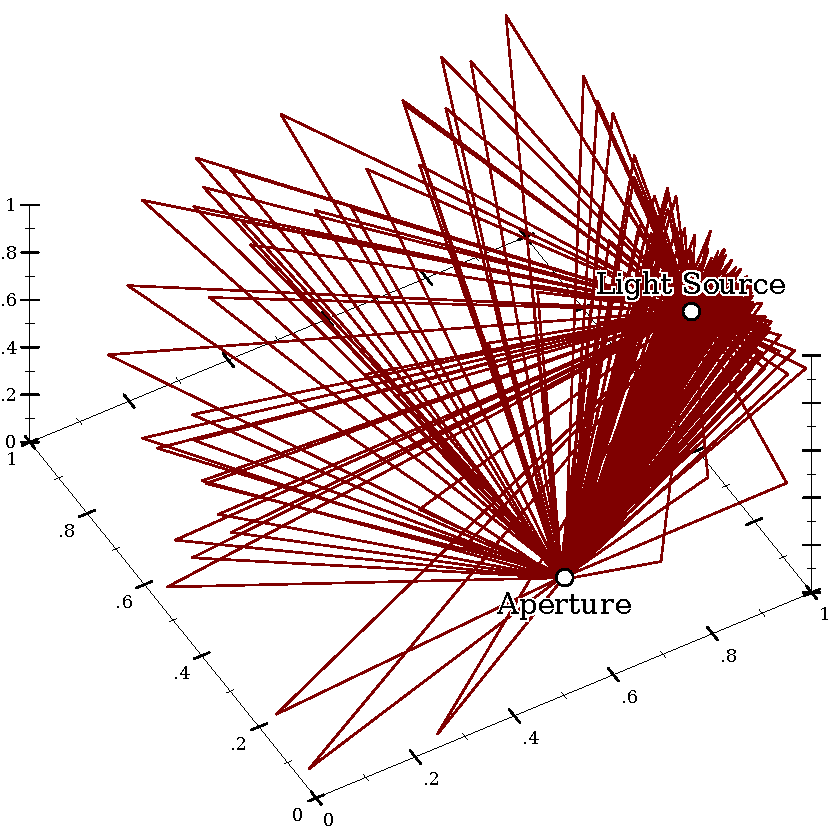
\includegraphics[width=\textwidth]{ray-tracing}
\end{minipage}
\label{fig:ray-tracing-paths}
}
\tab\tab
\subfloat[Random paths that pass through the aperture, projected onto a plane and accumulated.]{
\begin{minipage}{0.43\textwidth}
\centering
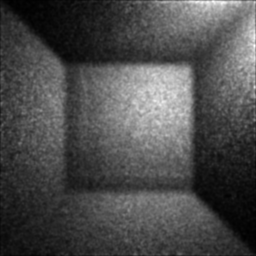
\includegraphics[width=\textwidth]{ray-tracing-projection}
\end{minipage}
\label{fig:ray-tracing-projection}
}

\subfloat[Part of the ray tracer implementation. Sampling involves computing approximate preimages under functions like this.]{
\usebox{\codebox}
\label{fig:ray-plane-intersect}
}
\caption[Stochastic ray tracing in Dr. Bayes]{Stochastic ray tracing in Dr. Bayes is little more than physics simulation.}
\label{fig:ray-tracing}
\end{figure*}

\figref{fig:ray-tracing} shows the result of using Dr. Bayes for stochastic ray tracing~\cite{cit:veach-1997siggraph-mlt}.
In this instance, photons are cast from a light source in a uniformly random direction and are reflected by the walls of a square room, generating paths.
The objective is to sample, with the correct distribution, only those paths that pass through an aperture.
The smaller the aperture, the smaller the probability a path passes through it, and the more focused the resulting image.

All efficient implementations of stochastic ray tracing to date use sophisticated, specialized sampling methods that bear little resemblance to the physical processes they simulate.
The proof-of-concept ray tracer, written in Dr. Bayes, is little more than a simple physics simulation and a conditional query.


%%%%%%%%%%%%%%%%%%%%%%%%%%%%%%%%%%%%%%%%%%%%%%%%%%%%%%%%%%%%%%%%%%%%%%%%%%%%%%%%%%%%%%%%%%%%%%%%%%%%%
%%%%%%%%%%%%%%%%%%%%%%%%%%%%%%%%%%%%%%%%%%%%%%%%%%%%%%%%%%%%%%%%%%%%%%%%%%%%%%%%%%%%%%%%%%%%%%%%%%%%%
%%%%%%%%%%%%%%%%%%%%%%%%%%%%%%%%%%%%%%%%%%%%%%%%%%%%%%%%%%%%%%%%%%%%%%%%%%%%%%%%%%%%%%%%%%%%%%%%%%%%%

\section{Related Work}

Any programming language research described by the words ``bijective'' or ``reversible'' might seem to have much in common with ours.
Unfortunately, when we look more closely, we can usually draw only loose analogies and perhaps inspiration.
An example is lenses~\cite{cit:hofmann-2012popl-edit-lenses}, which are transformations from $X$ to $Y$ that can be run forward and backward, in a way that maintains some relationship between $X$ and $Y$.
Usually, a destructive, external process is assumed, so that, for example, a change from $y \in Y$ to $y' \in Y$ induces a corresponding change from $x \in X$ to some $x' \in X$.
When transformations lose information, lenses must satisfy certain behavioral laws.
In our work, no input or output is updated, and preimages are always definable regardless of non-injectivity.

Many multi-paradigm languages~\cite{cit:hanus-2007lp-multi-paradigm}, especially constraint functional languages, bear a strong resemblance to our work.
In fact, it is easy to add a $fail$ expression to our semantics, or to transform constraints into boolean program outputs.
The most obvious difference is evaluation strategy.
The most important difference is that our interpretation of programs returns \emph{distributions} of constrained outputs, rather than arbitrary single values that meet constraints.

The forward phase in computing preimages takes a subdomain and returns an overapproximation of the function's range for that subdomain.
This clearly generalizes interval arithmetic~\cite{cit:kearfott-1996eb-interval} to all first-order algebraic types.

Our approximating semantics can be regarded as an abstract interpretation~\cite{cit:cousot-1977popl-abstract-interpretation} where the concrete domain consists of measurable sets and the abstract domain consists of rectangular sets.
In some ways, it is quite typical: it is sound, it labels expressions, the abstract domain is a lattice, and the exact semantics it approximates performs infinite computations.
However, it is far from typical in other ways.
It is used to run programs, not for static analysis.
The abstraction boundaries are the $if$ branches of completely unrolled, infinite programs, and are not fixed.
There is no Kleene iteration.
Infinite computations are done in a library of \lzfclang-computable combinators, not by a semantic function.
This cleanly separates the syntax from the semantics, and allows us to prove the exact semantics correct mostly by proving simple categorical properties.

Probabilistic languages can be approximately placed into two groups: those defined by an implementation, and those defined by a semantics.

Some languages defined by an implementation are a probabilistic Scheme by Koller and Pfeffer~\cite{cit:koller-1997aaai-bayes-programs-short}, BUGS~\cite{cit:winbugs-language-short}, BLOG~\cite{cit:blog-language-short}, BLAISE~\cite{cit:blaise-language}, Church~\cite{cit:church-language-short}, and Kiselyov's embedded language for O'Caml based on continuations~\cite{cit:kiselyov-2008uai-monolingual}.
The reports on these languages generally describe interpreters, compilers, and algorithms for sampling with probabilistic conditions.
Recently, Wingate et al~\cite{cit:wingate-2011ais-lightweight,cit:wingate-2011nips-nonstandard} have defined the semantics of \emph{nonstandard interpretations} that enable efficient inference, but do not define the languages.

Early work in probabilistic language semantics is not motivated by Bayesian concerns, and thus does not address conditioning.
Kozen~\cite{cit:kozen-1979fcs-prob-programs-short} defines the meaning of bounded-space, imperative ``while'' programs as functions from probability measures to probability measures.
Hurd~\cite{cit:hurd-2002thesis} proves properties about programs with binary random choice by encoding programs and portions of measure theory in HOL.
Jones~\cite{cit:jones-1990thesis} develops a domain-theoretic variation of probability theory, and with it defines the probability monad, whose discrete version is a distribution-valued variation of the set or list monad.
Ramsey and Pfeffer~\cite{cit:ramsey-2002popl-stochastic-short} define the probability monad measure-theoretically and implement a language for finite probability.
Park~\cite{cit:park-2008toplas-prob} extends a $\lambda$-calculus with probabilistic choice from a general class of probability measures using inverse transform sampling.

Some recent work in probabilistic language semantics tackles conditioning. Pfeffer's IBAL~\cite{cit:pfeffer-2007chapter-ibal} is the earliest lambda calculus with finite probabilistic choice that also defines conditional queries.
Borgstr\"om et al~\cite{cit:borgstrom-2011esop-measure-transformer} develop Fun, a first-order functional language without recursion, extended with probabilistic choice and conditioning.
Its semantics interprets programs as \emph{measure transformers} by transforming expressions into arrow-like combinators.
The implementation generates a decomposition of the probability density represented by the program, if it exists.
Bhat et al~\cite{cit:bhat-2013etaps-densities} replaces Fun's $if$ with $match$, and interprets programs more directly as probability density functions by compositionally transforming expressions into an extension of the probability monad.


%%%%%%%%%%%%%%%%%%%%%%%%%%%%%%%%%%%%%%%%%%%%%%%%%%%%%%%%%%%%%%%%%%%%%%%%%%%%%%%%%%%%%%%%%%%%%%%%%%%%%
%%%%%%%%%%%%%%%%%%%%%%%%%%%%%%%%%%%%%%%%%%%%%%%%%%%%%%%%%%%%%%%%%%%%%%%%%%%%%%%%%%%%%%%%%%%%%%%%%%%%%
%%%%%%%%%%%%%%%%%%%%%%%%%%%%%%%%%%%%%%%%%%%%%%%%%%%%%%%%%%%%%%%%%%%%%%%%%%%%%%%%%%%%%%%%%%%%%%%%%%%%%

\section{Conclusions and Future Work}

To allow recursion and arbitrary conditions in probabilistic programs, we combined the power of measure theory with the unifying elegance of arrows. We
\begin{enumerate}
	\item Defined a transformation from first-order programs to arbitrary arrows.
	\item Defined the bottom arrow as a standard translation target.
	\item Derived the uncomputable preimage arrow as an alternative target.
	\item Derived a sound, computable approximation of the preimage arrow, and enough computable lifts to transform programs.
\end{enumerate}
Critically, the preimage arrow's lift from the bottom arrow distributes over bottom arrow computations.
Our semantics thus generalizes this process to all programs: 1) encode a program as a bottom arrow computation; 2) lift this computation to get an uncomputable function that computes preimages; 3) distribute the lift; and 4) replace uncomputable expressions with sound approximations.

Our semantics trades efficiency for simplicity by threading a constant, tree-shaped random source (Section~\ref{sec:threading-and-indexing}).
Passing subtrees instead would make $random$ a constant-time primitive, and allow combinators to detect lack of change and return cached values.
Other future optimization work includes creating new sampling algorithms, and using other easily measured but more expressive set representations, such as parallelotopes~\cite{cit:amato-2012tcs-parallelotopes}.
On the theory side, we intend to explore preimage computation's connection to type checking and type inference, investigate ways to integrate and leverage polymorphic type systems, and find the conditions under which preimage refinement is complete in the limit.

More broadly, we hope to advance Bayesian practice by providing a rich modeling language with an efficient, correct implementation, which allows general recursion and any computable, probabilistic condition.

%%%%%%%%%%%%%%%%%%%%%%%%%%%%%%%%%%%%%%%%%%%%%%%%%%%%%%%%%%%%%%%%%%%%%%%%%%%%%%%%%%%%%%%%%%%%%%%%%%%%%
%%%%%%%%%%%%%%%%%%%%%%%%%%%%%%%%%%%%%%%%%%%%%%%%%%%%%%%%%%%%%%%%%%%%%%%%%%%%%%%%%%%%%%%%%%%%%%%%%%%%%
%%%%%%%%%%%%%%%%%%%%%%%%%%%%%%%%%%%%%%%%%%%%%%%%%%%%%%%%%%%%%%%%%%%%%%%%%%%%%%%%%%%%%%%%%%%%%%%%%%%%%

\mathversion{normal}



\chapter{Implementation of Preimage Computation}

\mathversion{sans}

\DeclarePairedDelimiter{\ivl}{[\mspace{-4.5mu}(}{)\mspace{-4.5mu}]}

\section{Set Representation}


\section{Preimages Under Real Functions}

\newcommand{\cl}[1]{\overline{\vphantom{i}{#1}}}
\newcommand{\sub}[1]{_{_{#1}}}

XXX: lifts are generally uncomputable, but many specific lifts are computable or approximately computable

XXX: something about computing functions backward by computing inverses forward

XXX: obvious how to do this with invertible functions (though infinite endpoints are a little tricky); not obvious how to do the same with two-argument functions

\subsection{Invertible Primitives}

We consider only strictly monotone functions on $\Re$.
Further on, we recover more generality by using language conditionals to implement \emph{piecewise} monotone functions.

One reason we consider only strictly monotone functions is that they are easy to invert.
Recall that a function is invertible (bijective) if and only if it is injective (one-to-one) and surjective (onto).

\begin{lemma}
\label{lem:monotone-implies-invertible}
If $f : A \to B$ is strictly montone, $f$ is injective.
If $f$ is additionally surjective, $f$ and its inverse are continuous.
\end{lemma}

Preimages under invertible functions can be computed using their inverses.
We are primarily interested in computing preimages under restricted functions.

\begin{lemma}
\label{lem:invertible-function-preimages}
Let $A' \subseteq A$, $B' \subseteq B$, and $f : A \to B$ have inverse $f^{-1} : B \to A$.
Let $f' := restrict~f~A'$. Then
\begin{equation}
	preimage~f'~B'\ =\ A' \i image~f^{-1}~B'
\end{equation}
\end{lemma}

\begin{figure}[!tb]
\centering
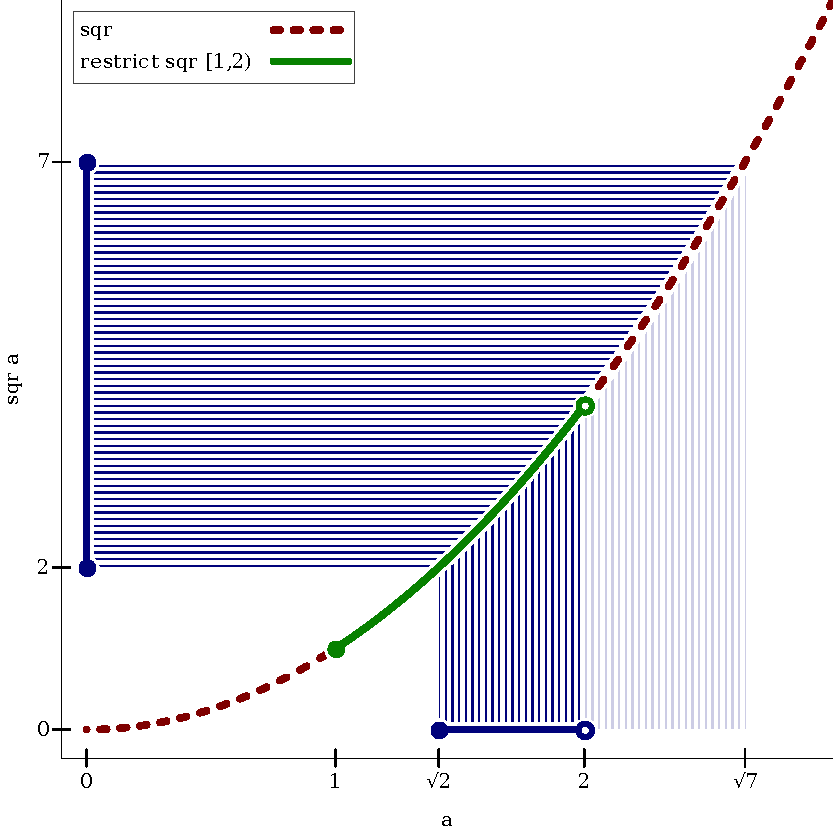
\includegraphics[width=4in]{preimage-by-inverse-image}
\caption[ ]{Computing the preimage of the interval $[2,7]$ under $sqr$ restricted to $[1,2)$, by computing roots and intersecting with $[1,2)$.}
\label{fig:sqr-preimage}
\end{figure}

These facts suggest that we can compute images (or preimages) of intervals under any strictly monotone, surjective $f$ by applying $f$ (or its inverse) to interval endpoints to yield an interval, as in Figure~\ref{fig:sqr-preimage}
This is evident for endpoints in $A$.
Limit endpoints like $+\infty$ require a larger $\cl{f}$ defined on a compact superset of $A$.

The next theorem is easier to state with interval notation in which the kind of interval is not baked into the syntax.

\begin{definition}[interval]
$\ivl{a_1,a_2,\alpha_1,\alpha_2}$ denotes an interval, where $a_1,a_2 \in \cl{\Re}$ are extended real endpoints, and $\alpha_1,\alpha_2 \in Bool$ determine whether $a_1$ and $a_2$ are contained in the interval.
\end{definition}

\begin{example}
Some intervals, using $\ivl{\cdot,\cdot,\cdot,\cdot}$ notation:
\begin{equation}
\begin{aligned}
	\ivl{0,1,true,false} &= [0,1) \\
	\ivl{-\infty,0,false,true} &= (-\infty,0] \\
	\ivl{-\infty,+\infty,false,false} &= (-\infty,+\infty) = \Re \\
	\ivl{-\infty,+\infty,true,true} &= [-\infty,+\infty] = \cl{\Re}
\end{aligned}
\end{equation}
All but the last are subsets of $\Re$.
\exampleqed
\end{example}

\begin{theorem}[images of intervals by endpoints]
\label{thm:images-of-intervals}
Let $\cl{A}$ and $\cl{B}$ be compact subsets of $\cl{\Re}$, $\cl{f} : \cl{A} \to \cl{B}$ strictly monotone and surjective, and $f$ the restriction of $\cl{f}$ to some $A \subseteq \cl{A}$.
For all nonempty $\ivl{a_1,a_2,\alpha_1,\alpha_2} \subseteq A$,
\begin{itemize}
	\item If $\cl{f}$ is increasing, $image~f~\ivl{a_1,a_2,\alpha_1,\alpha_2} = \ivl{\cl{f}~a_1, \cl{f}~a_2,\alpha_1,\alpha_2}$.
	\item If $\cl{f}$ is decreasing, $image~f~\ivl{a_1,a_2,\alpha_1,\alpha_2} = \ivl{\cl{f}~a_2, \cl{f}~a_1,\alpha_2,\alpha_1}$.
\end{itemize}
\end{theorem}
\begin{proof}
Because $\cl{A}$ is compact and totally ordered, every subset of $\cl{A}$ has a lower and an upper bound in $\cl{A}$.
Therefore, the endpoints of every interval subset of $A$ are in $\cl{A}$.

Let $(a_1,a_2] \subseteq A$.
Suppose $\cl{f}$ is strictly increasing; thus $a_1 < a \leq a_2$ if and only if $\cl{f}~a_1 < \cl{f}~a \leq \cl{f}~a_2$, so $image~f~(a_1,a_2] = image~\cl{f}~(a_1,a_2] = (\cl{f}~a_1,\cl{f}~a_2]$.
The remaining cases are similar.
\end{proof}

To use Theorem~\ref{thm:images-of-intervals} to compute preimages under $f$ by computing images under its inverse $f^{-1}$, we must know whether $f^{-1}$ is increasing or decreasing.
The following lemma can help.

\begin{lemma}
\label{lem:inverse-direction}
If $f : A \to B$ is strictly monotone and surjective with inverse $f^{-1} : B \to A$, then $f$ is increasing if and only if $f^{-1}$ is increasing.
\end{lemma}

\begin{example}
The extension of $log : (0,+\infty) \to \Re$ to the compact superdomain $[0,+\infty]$ is defined by
\begin{equation}
\begin{aligned}
	&\cl{log} : [0,+\infty] \to \cl{\Re} \\
	&	\cl{log}~a\ := \lim_{a' \to a} log~a'
		\ =\ \lzfccase{a}{
				0 & -\infty \\
				+\infty & +\infty \\
				else & log~a \\
			}
\end{aligned}
\end{equation}
The extension of its inverse $exp$ is $\cl{exp} : \cl{\Re} \to [0,+\infty]$, defined similarly, which by Lemma~\ref{lem:inverse-direction} is also strictly increasing.
Thus,
\begin{equation}
\begin{aligned}
	image~log~(0,1]\ &=\ (\cl{log}~0,\cl{log}~1] = (-\infty,0]
\\[0.5\baselineskip]
	preimage~log~[0,+\infty)
		\ &=\ image~exp~[0,+\infty)
\\
		\ &=\ [\mspace{2mu}\cl{exp}~0,\cl{exp}~{+\infty})
		= [1,+\infty)
\end{aligned}
\end{equation}
by Theorem~\ref{thm:images-of-intervals} and Lemma~\ref{lem:invertible-function-preimages},
\exampleqed
\end{example}

%%%%%%%%%%%%%%%%%%%%%%%%%%%%%%%%%%%%%%%%%%%%%%%%%%%%%%%%%%%%%%%%%%%%%%%%%%%%%
%%%%%%%%%%%%%%%%%%%%%%%%%%%%%%%%%%%%%%%%%%%%%%%%%%%%%%%%%%%%%%%%%%%%%%%%%%%%%
%%%%%%%%%%%%%%%%%%%%%%%%%%%%%%%%%%%%%%%%%%%%%%%%%%%%%%%%%%%%%%%%%%%%%%%%%%%%%

\subsection{Two-Argument Primitives}

We do not expect to be able to compute preimages under $\Re \times \Re \pto \Re$ primitives by simply inverting them.
Two-argument invertible real functions are difficult to define and are usually pathological.

Instead, we compute approximate preimages only, using inverses with respect to one argument (with the other held constant).

\begin{definition}[axial inverse]
\label{def:axial-inverse}
Let $f_c : A \times B \to C$.
Functions $f_a : B \times C \to A$ and $f_b : C \times A \to B$ defined so that
\begin{equation}
	f_c~\pair{a,b} = c\ \iff\ f_a~\pair{b,c} = a\ \iff\ f_b~\pair{c,a} = b
\end{equation}
are \mykeyword{axial inverses} with respect to $f_c$'s first and second arguments.
\end{definition}

We call $f_c$ \mykeyword{axis-invertible} or \mykeyword{trijective} when it has axial inverses $f_a$ and $f_b$.
We call $f_a$ the \mykeyword{first axial inverse} of $f_c$ because it is the inverse of $f_c$ along the first axis: $f_a$ with only $c$ varying (i.e. $\fun{c \in C} f_a~\pair{b,c}$), is the inverse of $f_c$ with only $a$ varying (i.e. $\fun{a \in A} f_c~\pair{a,b}$).
Similarly, $f_b$ is the \mykeyword{second axial inverse}.

\begin{example}
\label{ex:plus-axial-inverses}
Let $add_c : \Re \times \Re \to \Re$, $add_c~\pair{a,b} := a+b$.
Its axial inverses are $add_a~\pair{b,c} := c - b$ and $add_b~\pair{c,a} := c - a$.
\exampleqed
\end{example}

We have chosen the axial inverse function types carefully: they are the only types for which $f_c$, $f_a$ and $f_b$ form a cyclic group.

\begin{lemma}
\label{lem:axial-inverse-cyclic-group}
The following statements are equivalent.
\begin{itemize}
	\item $f_c$ has axial inverses $f_a$ and $f_b$.
	\item $f_a$ has axial inverses $f_b$ and $f_c$.
	\item $f_b$ has axial inverses $f_c$ and $f_a$.
\end{itemize}
Equivalently, every axis-invertible function generates a cyclic group of order 3 by inversion in the first axis.
\end{lemma}

This fact is analogous to how mutual inverses $f$ and $f^{-1}$ also form a cyclic group (of order 2, generated by inversion).
Similar to using mutual inversion to compute preimages under both $log$ and $exp$, Lemma~\ref{lem:axial-inverse-cyclic-group} allows computing preimages under two-argument functions related by axial inversion.

\begin{example}
Define $sub_c : \Re \times \Re \to \Re$ by $sub_c~\pair{a,b} := a-b$.
Because $sub_c = add_b$, $sub_a = add_c$ and $sub_b = add_a$.
\exampleqed
\end{example}

Unlike inverses, axial inverses do not provide a direct way to compute exact preimages.
Instead, they provide a way to compute a preimage's smallest rectangular bounding set.

\begin{theorem}[preimage bounds from axial inverse images]
\label{thm:axis-invertible-function-preimages}
Let $A' \subseteq A$, $B' \subseteq B$, $C' \subseteq C$, and $f_c : A \times B \to C$ with axial inverses $f_a$ and $f_b$.
If $f_c' = restrict~f_c~(A' \times B')$, then
\begin{equation}
	preimage~f_c'~C'\ \subseteq\ \lzfcsplit{
		&(A' \i image~f_a~(B' \times C'))\ \times \\
		&(B' \i image~f_b~(C' \times A'))}
\end{equation}
Further, the right-hand side is the smallest rectangular superset.
\end{theorem}
\begin{proof}
The smallest rectangle containing $preimage~f_c'~C'$ is
\begin{equation}
	preimage~f_c'~C'\ \subseteq\ 
		\lzfcsplit{
			&(image~fst~(preimage~f_c'~C'))\ \times \\
			&(image~snd~(preimage~f_c'~C'))}
\end{equation}
Starting with the first set in the product, expand definitions, distribute $fst$, replace $f_c~\pair{a,b} = c$ by $f_a~\pair{b,c} = a$, and simplify:
\begin{displaybreaks}
\begin{align*}
	&image~fst~(preimage~f_c'~C')
\nobreak\\
	&\tab =\ image~fst~\setb{\pair{a,b} \in A' \times B'}{f_c~\pair{a,b} \in C'}
\\
	&\tab =\ \setb{a \in A'}{\Exists{b \in B'} f_c~\pair{a,b} \in C'}
\\
	&\tab =\ \setb{a \in A'}{\Exists{b \in B',c \in C'} f_c~\pair{a,b} = c}
\\
	&\tab =\ \setb{a \in A'}{\Exists{b \in B',c \in C'} f_a~\pair{b,c} = a}
\\
	&\tab =\ \setb{f_a~\pair{b,c}}{b \in B', c \in C', f_a~\pair{b,c} \in A'}
\\
	&\tab =\ A' \i \setb{f_a~\pair{b,c}}{b \in B', c \in C'}
\nobreak\\
	&\tab =\ A' \i image~f_a~(B' \times C')
\end{align*}
\end{displaybreaks}
The second set in the product is similar.
\end{proof}

\begin{figure}[!tb]
\centering
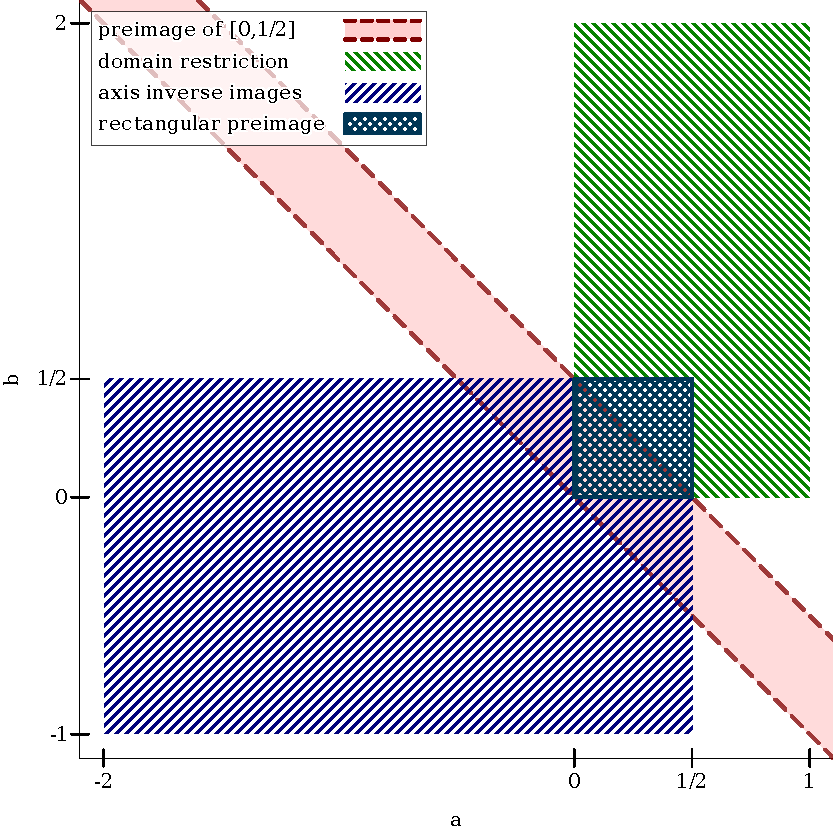
\includegraphics[width=4in]{rect-preimage-by-inverse-images}
\caption[ ]{Computing an approximate preimage of $[0,\tfrac{1}{2}]$ under addition restricted to $[0,1] \times [0,2]$ (Example~\ref{ex:plus-preimage}).
The preimage is approximated by intersecting the domain with an overapproximation computed using axial inverses.}
\label{fig:plus-preimage}
\end{figure}

\begin{example}
\label{ex:plus-preimage}
See Figure~\ref{fig:plus-preimage}.
Let $add_c' := restrict~add_c~([0,1] \times [0,2])$.
By Theorem~\ref{thm:axis-invertible-function-preimages},
\begin{align*}
	preimage~add_c'~[0,\tfrac{1}{2}]
		&\subseteq \lzfcsplit{
			&([0,1] \i image~add_a~([0,2] \times [0,\tfrac{1}{2}]))\ \times \\
			&([0,2] \i image~add_b~([0,\tfrac{1}{2}] \times [0,1]))}
\\
		&= ([0,1] \i [-2,\tfrac{1}{2}]) \times ([0,2] \i [-1,\tfrac{1}{2}])
\\
		&= [0,\tfrac{1}{2}] \times [0,\tfrac{1}{2}]
\end{align*}
is the smallest rectangular subset of $[0,1] \times [0,2]$ that contains the preimage of $[0,\tfrac{1}{2}]$ under $add_c$.
\exampleqed
\end{example}

At this point, we have an analogue of Lemma~\ref{lem:invertible-function-preimages}, in that we can compute (approximate) preimages by computing images under (axial) inverses.
To compute images using interval endpoints, we need analogues of Lemma~\ref{lem:monotone-implies-invertible} (strictly monotone, surjective functions are invertible and continuous), Theorem~\ref{thm:images-of-intervals} (images of intervals by endpoints), and Lemma~\ref{lem:inverse-direction} (inverse direction).

We first need a notion of properties that hold along an axis for every fixed value of the other argument.

\begin{definition}[uniform axis property]
$f_c : A \times B \to C$ has property $P$ \keyword{uniformly} in its first axis when $P~(flip~(curry~f_c)~b)$ for all $b \in B$, and uniformly in its second axis when $P~(curry~f_c~a)$ for all $a \in A$.
If the axis is not specified, $P$ holds uniformly for both.
\end{definition}

Now Lemma~\ref{lem:monotone-implies-invertible}'s analogue is an easy corollary.

\begin{lemma}
\label{lem:uniformly-monotone-implies-invertible}
Let $f_c : A \times B \to C$ for totally ordered $A$, $B$ and $C$.
If $f_c$ is uniformly surjective and either uniformly strictly increasing or uniformly strictly decreasing in each axis, then $f_c$ is axis-invertible; further, it and its axial inverses are continuous.
\end{lemma}

From here on, assume axis monotonicity properties are uniform unless otherwise stated.

\begin{example}
$add_c$ is uniformly surjective and strictly increasing.
$sub_c$ is uniformly surjective and strictly increasing/decreasing in its first/second axis.
Therefore, both are axis-invertible.
\exampleqed
\end{example}

Restriction usually makes a function not uniformly surjective.

\begin{example}
Let $add_c' : [0,1] \times [0,1] \to [0,2]$, defined by restricting $add_c$.
It is strictly increasing, but not uniformly surjective: the range of $curry~add_c'~0$ is $[0,1]$, not $[0,2]$.
\exampleqed
\end{example}

\begin{figure}[!tb]
\centering
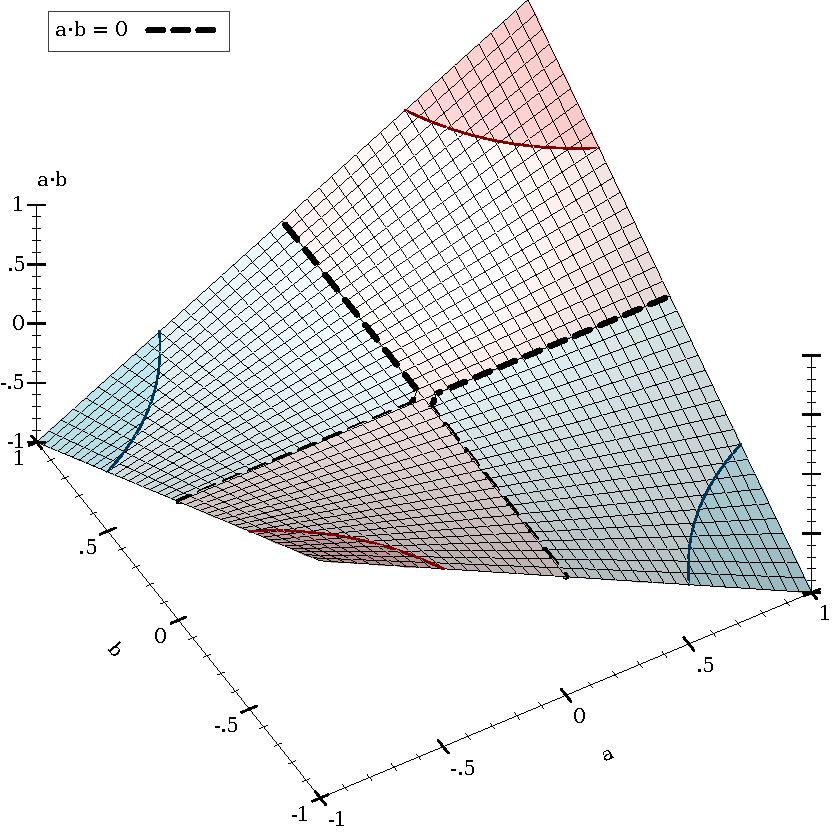
\includegraphics[width=4in]{mul-nonuniform-properties}
\caption[ ]{Multiplication on $\Re \times \Re$ is not uniformly surjective, nor uniformly strictly increasing or decreasing in each axis: $a \cdot 0 = 0$ and $0 \cdot b = 0$ for all $a$ and $b$ (Example~\ref{ex:mul-nonuniform}).
Fortunately, it is uniformly surjective and strictly monotone in each open quadrant.}
\label{fig:mul-nonuniform}
\end{figure}

Fortunately, restriction sometimes does the opposite.

\begin{example}
\label{ex:mul-nonuniform}
Define $mul_c : \Re \times \Re \to \Re$ by $mul_c~\pair{a,b} := a \cdot b$.
It is not uniformly surjective nor strictly monotone because $mul_c~\pair{0,b} = 0$ for all $b \in B$.
(See Figure~\ref{fig:mul-nonuniform}.)
But $mul_c^{++} : (0,+\infty) \times (0,+\infty) \to (0,+\infty)$, and $mul_c$ restricted to the other open quadrants, are uniformly surjective and strictly increasing or decreasing in each axis.
\exampleqed
\end{example}

Theorem~\ref{thm:images-of-intervals} justifies computing images of intervals with infinite endpoints by applying an extended function to the endpoints.
Its two-argument analogue is more involved because extended, two-argument functions may not be defined at every point.

\begin{example}
$add_c$ cannot be extended to $\cl{add_c} : \cl{\Re} \times \cl{\Re} \to \cl{\Re}$ in the same way $log$ is extended to $\cl{log}$ because
\begin{equation}
	\lim_{\pair{a',b'} \to \pair{a,b}} add_c~\pair{a',b'}
\end{equation}
does not exist when $\pair{a,b}$ is $\pair{-\infty,+\infty}$ or $\pair{+\infty,-\infty}$.
\exampleqed
\end{example}

The previous example suggests that extensions of increasing, two-argument functions are always well-defined except at off-diagonal corners.
This is true, and similar statements hold for axes with other directions, and for more restricted domains.

\begin{theorem}[$\cl{\Re} \times \cl{\Re}$ extension]
\label{thm:two-argument-extensions}
Let $A$, $B$, $C$ be open subsets of $\Re$, with $f_c : A \times B \to C$ uniformly surjective and strictly increasing or decreasing in each axis.
Let $\cl{A}$, $\cl{B}$ and $\cl{C}$ be the closures of $A$, $B$ and $C$ in $\cl{\Re}$.
The following extension is well-defined:
\begin{equation}
\begin{aligned}
	&\cl{f_c} : (\cl{A} \times \cl{B}) \w N \to \cl{C} \\
	&\cl{f_c}~\pair{a,b}\ :=\ \lim_{\pair{a',b'} \to \pair{a,b}} f_c~\pair{a',b'}
\end{aligned}
\end{equation}
where $N := \set{\pair{min~\cl{A},max~\cl{B}},\pair{max~\cl{A},min~\cl{B}}}$ if $f_c$ is increasing or decreasing, and
$N := \set{\pair{min~\cl{A},min~\cl{B}},\pair{max~\cl{A},max~\cl{B}}}$ if $f_c$ is increasing/decreasing or decreasing/increasing.
\end{theorem}
\begin{proof}
Suppose $f_c$ is increasing, and let $g : \Nat \to A \times B$ be a sequence of $f_c$'s domain values.

Any $g$ that converges to $\pair{max~\cl{A},max~\cl{B}}$ has a strictly increasing subsequence.
By monotonicity, $map~f_c~g$ has a strictly increasing subsequence.
It is bounded by $max~\cl{C}$, so $\cl{f_c}~\pair{max~\cl{A},max~\cl{B}} = max~\cl{C}$.
A similar argument proves $\cl{f}~\pair{min~\cl{A},min~\cl{B}} = min~\cl{C}$.

For any $g$ that converges to $\pair{max~\cl{A},b'}$ for some $b' \in B$, define
\begin{equation}
	g'\ :=\ map~(\fun{\pair{a,b}}\pair{f_a~\pair{b',f_c~\pair{a,b}}',b'})~g
\end{equation}
where $f_a$ is $f_c$'s first axial inverse, so that $map~f_c~g = map~f_c~g'$.
Because $g'$ has a subsequence that is strictly increasing in the first of each pair, and because the second of each pair is the constant $b'$, by monotonicity, $map~f_c~g'$ has a strictly increasing subsequence.
It is bounded by $max~\cl{C}$, so $\cl{f_c}~\pair{max~\cl{A},b'} = max~\cl{C}$.
By similar arguments, $\cl{f}~\pair{min~\cl{A},b} = min~\cl{C}$ and so on.

Arguments for $f$ decreasing, etc., are similar.
\end{proof}

Following the proof of Theorem~\ref{thm:two-argument-extensions}, extensions of two-argument functions can be defined by two corner cases, four border cases, and an interior case.

\begin{example}
Define $pow_c : (0,1) \times (0,+\infty) \to (0,1)$ by $pow_c~\pair{a,b} := exp~(b \cdot log~a)$, which is increasing/decreasing.
Its extension to a subset of $\cl{\Re} \times \cl{\Re}$ is
\begin{equation}
\begin{aligned}
	&\cl{pow_c} : ([0,1] \times [0,+\infty]) \w N \to [0,1] \\
	&\cl{pow_c}~\pair{a,b}\ :=\
		\lzfccase{\pair{a,b}}{
			\pair{0,+\infty} & 0 \\
			\pair{1,0} & 1 \\ 
			\pair{0,b} & 0 \\
			\pair{1,b} & 1 \\
			\pair{a,0} & 1 \\
			\pair{a,+\infty} & 0 \\
			else & pow_c~\pair{a,b}
		}
\end{aligned}
\end{equation}
where $N := \set{\pair{0,0},\pair{1,+\infty}}$.
\exampleqed
\end{example}

The analogue of Theorem~\ref{thm:images-of-intervals} is easiest to state if we have predicates that indicate a function's direction in each axis.
Define $inc_1 : (A \times B \to C) \tto Bool$ so that $inc_1~f$ if and only if $f$ is strictly increasing in its first axis, and similarly $inc_2$ so that $inc_2~f$ if and only if $f$ is strictly increasing in its second axis.

\begin{theorem}[images of rectangles by interval endpoints]
\label{thm:images-of-rectangles}
Let $A,B,C$ be open subsets of $\Re$, with $f_c : A \times B \to C$ uniformly surjective and strictly increasing or decreasing in each axis, with extension $\cl{f_c}$ as defined in Theorem~\ref{thm:two-argument-extensions}.
If $A' := \ivl{a_1,a_2,\alpha_1,\alpha_2} \subseteq A$ and $B' := \ivl{b_1,b_2,\beta_1,\beta_2} \subseteq B$, then the image $C'$ under $f_c$ is
\begin{equation}
\begin{aligned}
	&image~f_c~(\ivl{a_1,a_2,\alpha_1,\alpha_2} \times \ivl{b_1,b_2,\beta_1,\beta_2})
\\
	&\tab =\ \lzfclet{
		\pair{a_1,a_2,\alpha_1,\alpha_2} & \lzfccond{(inc_1~f_c) & \pair{a_1,a_2,\alpha_1,\alpha_2} \\ else & \pair{a_2,a_1,\alpha_2,\alpha_1}} \\
		\pair{b_1,b_2,\beta_1,\beta_2} & \lzfccond{(inc_2~f_c) & \pair{b_1,b_2,\beta_1,\beta_2} \\ else & \pair{b_2,b_1,\beta_2,\beta_1}}
	}{\ivl{\cl{f_c}~\pair{a_1,b_1},\cl{f_c}~\pair{a_2,b_2},\alpha_1~and~\beta_1,\alpha_2~and~\beta_2}}
\end{aligned}
\end{equation}
\end{theorem}
\begin{proof}
Because $f_c$ is continuous and $A' \times B'$ is a connected set, $C'$ is a connected set, which in $\Re$ is an interval.
Thus, we need to determine only its bounds and whether it contains each endpoint.

Suppose $f_c$ is increasing.
By monotonicity, $C'$ is contained in $[\cl{f_c}~\pair{a_1,b_1},\cl{f_c}~\pair{a_2,b_2}]$.
If either $\alpha_1$ or $\beta_1$ is $false$, $C'$ cannot contain $\cl{f_c}~\pair{a_1,b_1}$.
If either $\alpha_2$ or $\beta_2$ is $false$, $C'$ cannot contain $\cl{f_c}~\pair{a_2,b_2}$.
Therefore $C' = \ivl{\cl{f_c}~\pair{a_1,b_1},\cl{f_c}~\pair{a_2,b_2},\alpha_1~and~\beta_1,\alpha_2~and~\beta_2}$.

We still must prove $\pair{a_1,b_1}$ and $\pair{a_2,b_2}$ are in $\cl{f_c}$'s domain.
First, recall $\cl{f_c} : (\cl{A} \times \cl{B}) \w N \to \cl{C}$, where $\cl{A}$, $\cl{B}$ and $\cl{C}$ are the closures of $A$, $B$ and $C$ in $\cl{\Re}$, and $N = \set{\pair{min~\cl{A},max~\cl{B}},\pair{max~\cl{A},min~\cl{B}}}$.

Because $A' \subseteq A$ and $B' \subseteq B$, and $A$ and $B$ are open sets, $a_1 \neq max~\cl{A}$, $a_2 \neq \min~\cl{A}$, $b_1 \neq max~\cl{B}$, and $b_2 \neq min~\cl{B}$, so
\begin{equation}
\begin{aligned}
	\pair{a_1,b_1} &\neq \pair{max~\cl{A},b} & \text{for all}\ b \in \cl{B} \\
	\pair{a_1,b_1} &\neq \pair{a,max~\cl{B}} & \text{for all}\ a \in \cl{A} \\
	\pair{a_2,b_2} &\neq \pair{min~\cl{A},b} & \text{for all}\ b \in \cl{B} \\
	\pair{a_2,b_2} &\neq \pair{a,min~\cl{B}} & \text{for all}\ a \in \cl{A} \\
\end{aligned}
\end{equation}
Therefore, $\pair{a_1,b_1} \not\in N$ and $\pair{a_2,b_2} \not\in N$, as desired.

The remaining cases for $f_c$ are similar.
\end{proof}

\begin{example}
Because $inc_1~pow_c$ and $not~(inc_2~pow_c)$,
\begin{align*}
	&image~pow_c~((0,\tfrac{1}{2}] \times [2,+\infty))
\\
	&\ =\ \lzfclet{
		\pair{a_1,a_2,\alpha_1,\alpha_2} & \pair{0,\tfrac{1}{2},false,true} \\
		\pair{b_1,b_2,\beta_1,\beta_2} & \pair{+\infty,2,false,true}
	}{\ivl{\cl{pow_c}~\pair{a_1,b_1},\cl{pow_c}~\pair{a_2,b_2},\alpha_1~and~\beta_1,\alpha_2~and~\beta_2}}
\\
	&\ =\ \ivl{\cl{pow_c}~\pair{0,+\infty},\cl{pow_c}~\pair{\tfrac{1}{2},2},false~and~false,true~and~true}
\\
	&\ =\ \ivl{0,\tfrac{1}{4},false,true}
\\
	&\ =\ (0,\tfrac{1}{4}]
\\[-2.25\baselineskip]
\end{align*}
\exampleqed
\end{example}

To use Theorem~\ref{thm:images-of-rectangles} to compute approximate preimages under $f_c$ by computing images under its axial inverses, we must know whether each axis of $f_a$ and $f_b$ is increasing or decreasing.
It helps to have an analogue of Lemma~\ref{lem:inverse-direction} (inverse direction).

\begin{theorem}
Let $f_c : A \times B \to C$ be uniformly surjective and strictly increasing or decreasing in each axis, with axial inverses $f_a$ and $f_b$.
The following statements hold:
\begin{enumerate}
	\item $inc_1~f_a$ if and only if $(inc_1~f_c)~xor~(inc_2~f_c)$.
	\item $inc_2~f_a$ if and only if $inc_1~f_c$.
\end{enumerate}
\end{theorem}
\begin{proof}
For statement 1, let $c \in C$, $b_1,b_2 \in B$, $a_1 := f_a~\pair{b_1,c}$ and $a_2 := f_a~\pair{b_2,c}$.
Let $c' := f_c~\pair{a_1,b_2}$; note $c = f_c~\pair{a_1,b_1} = f_c~\pair{a_2,b_2}$.
Suppose $inc_1~f_c$ and $inc_2~f_c$; then $a_1 > a_2 \iff c < c'$ and $b_1 < b_2 \iff c < c'$, so $b_1 < b_2 \iff a_1 > a_2$.
The remaining cases are similar.

For statement 2, fix $b \in B$ and apply Lemma~\ref{lem:inverse-direction}.
\end{proof}

By Lemma~\ref{lem:axial-inverse-cyclic-group}, $inc_1~f_b \iff inc_2~f_c$, and $inc_2~f_b \iff inc_1~f_a$.
We can therefore easily determine the uniform directions of $f_a$'s and $f_b$'s axes from the uniform directions of $f_c$'s axes.

We are certain the preceeding definitions and theorems extend naturally to functions with any number of arguments, but have not needed to extend them yet.

%%%%%%%%%%%%%%%%%%%%%%%%%%%%%%%%%%%%%%%%%%%%%%%%%%%%%%%%%%%%%%%%%%%%%%%%%%%%%
%%%%%%%%%%%%%%%%%%%%%%%%%%%%%%%%%%%%%%%%%%%%%%%%%%%%%%%%%%%%%%%%%%%%%%%%%%%%%
%%%%%%%%%%%%%%%%%%%%%%%%%%%%%%%%%%%%%%%%%%%%%%%%%%%%%%%%%%%%%%%%%%%%%%%%%%%%%

\subsection{Discontinuous Primitives}

\section{Primitive Implementation}
\label{sec:primitive-implementation}

Because floating-point functions are defined on subsets of $\cl{\Re}$, it would seem we could compute preimages under strictly monotone, real functions by applying their floating-point counterparts to interval endpoints.
This is mostly true, but we must take care to round in the right directions and account for floating-point negative zero.

\begin{equation}
\begin{aligned}
	&\cl{pos!recip} : [0,+\infty] \to [0,+\infty] \\
	&\cl{pos!recip}~a\ =\
		\lzfccond{
			0 < a < +\infty & 1/a \\
			a = 0 & +\infty \\
			a = +\infty & 0
		}
\end{aligned}
\end{equation}

\section{Partitioned Sampling}

Suppose that we want to sample values in a probability space $X,P$ by first sampling a set from a \emph{partition} of $X$ and then sampling from that set.\footnote{This is not \emph{stratified} sampling, which samples a fixed number of times from each partition.}
[XXX: this transition should mention why we want to do partition sampling instead of just supposing that we do]

First, we define
\begin{equation}
\begin{aligned}
	&condition : Set~X \pto [0,1] \tto Set~X \tto Set~X \pto [0,1] \\
	&condition~P~A\ :=\ \fun{A' \in domain~P} P~(A' \i A)~{/}~P~A
\end{aligned}
\end{equation}
to restrict a probability measure $P$ to a measurable, positive-probability set $A$ and renormalize it.

\begin{definition}[partitioned sampling]
\label{def:partitioned-sampling}
Let $X,P$ be an arbitrary probability space, $N$ be an at-most-countable index set, and $s : N \to Set~X$ be a partition of $X$ into $|N|$ measurable parts. The following procedure samples from $X$:
\begin{enumerate}
	\item Choose $n \in N$ with probability $P~(s~n)$.
	\item Choose $a \in s~n$ according to $condition~P~(s~n)$.
\end{enumerate}
\end{definition}

It is not hard to show that partitioned sampling chooses an $a \in X$ according to $P$.

\begin{example}[partitioned sampling from a standard normal]
\label{ex:partitioned-sampling}
Let $P$ be the standard normal distribution's probability measure.
To sample according to $P$, let $N := \set{neg,pos}$ and $s = [neg \mapsto (-\infty,0], pos \mapsto (0,+\infty)]$, and define $Q : N \to Set~\Re \pto [0,1]$ by
\begin{equation}
\begin{aligned}
	Q~neg~A\ &=\ P~((-\infty,0] \i A)~{/}~\tfrac{1}{2} \\
	Q~pos~A\ &=\ P~((0,+\infty) \i A)~{/}~\tfrac{1}{2}
\end{aligned}
\end{equation}
Then
\begin{enumerate}
	\item Choose $n = neg$ or $n = pos$, each with probability $\frac{1}{2}$.
	\item Choose $a \in s~n$ according to $Q~n$.\exampleqed
\end{enumerate}
\end{example}

Partitioned sampling has two weaknesses.
First, it requires $P~(s~n)$ to be easy to compute for all $n \in N$.
If this were true, we would not need to sample in the first place---i.e. it assumes a solution to the overall problem we are trying to solve.
Second, it assumes sampling according to $condition~P~(s~n)$ is easy, which is also not reasonable, as sampling according to a conditioned distribution is a subproblem we are trying to solve.

But suppose we could easily sample a partition index according to a different distribution over $N$, and according to a different distribution over part $s~n$ for each $n \in N$. Doing so and returning weighted samples to adjust for the differences in distribution comprises \mykeyword{partitioned importance sampling}.

First, we define
\begin{equation}
\begin{aligned}
	&subcond : Set~X \pto [0,1] \tto Set~X \tto Set~X \pto [0,1] \\
	&subcond~P~A\ :=\ \fun{A' \in domain~P} P~(A' \i A)
\end{aligned}
\end{equation}
to restrict a probability measure $P$ to a measurable set $A$ \emph{without} renormalizing it; i.e. it returns a subprobability measure.

\begin{definition}[partitioned importance sampling]
\label{def:partitioned-importance-sampling}
Suppose we have
\begin{itemize}
	\item An arbitrary probability space $X,P$.
	\item An at-most-countable index set $N$.
	\item A probability mass function $p : N \to [0,1]$ such that $p~n > 0$ for all $n \in N$.
	\item A partition $s : N \to Set~X$ of $X$ into $|N|$ measurable parts.
	\item Candidate probability measures $Q : N \to Set~X \pto [0,1]$, one for each partition.
\end{itemize}
To sample from $X$ according to $P$,
\begin{enumerate}
	\item Choose $n \in N$ with probability $p~n$.
	\item Choose $a \in X$ according to $Q~n$.
	\item Compute $w := \dfrac{1}{p~n} \cdot diff^+~(subcond~P~(s~n))~(Q~n)~a$.
	\item Return the weighted sample $\pair{a,w}$.
\end{enumerate}
\end{definition}

The function $diff^+~(subcond~P~(s~n))~(Q~n)$, with type $X \to [0,+\infty)$, is a \keyword{Radon-Nikod\'ym\footnote{Pronounced ``RADon neekohDIM,'' and named after Austrian mathematician Johann Radon and Polish mathematician Otto Nikod\'ym.} derivative}.
If $P$ has density $f$, $Q~n$ has density $g$ with respect to the same base measure (e.g. same-dimensional length, area or volume), and $a \in s~n$ implies $g~a > 0$, then\footnote{The equality in~\eqref{eqn:diff-is-actually-easy} holds $(Q~n)$-almost everywhere.}
\begin{equation}
	diff^+~(subcond~P~(s~n))~(Q~n)~a\ =\ if~(a \in s~n)~(f~a~{/}~g~a)~0
\label{eqn:diff-is-actually-easy}
\end{equation}
Chapter~\ref{ch:sampling-algorithm-proofs} has definitions and more details.
We use $diff^+$ in a more general sense, but in this section, it is usually fine to think of its return values as quotients of densities.

An importance sampling algorithm is correct when all expected values computed using its weighted samples are the equal to the true expected values.
The next theorem states that this is true of partitioned importance sampling under reasonable conditions, which are analogous to the support of $subcond~P~(s~n)$ being no larger than that of $Q~n$.

\begin{theorem}[partitioned importance sampling correctness]
\label{thm:partitioned-importance-sampling-correctness}
Let $X$, $P$, $N$, $s$, $p$, and $Q$ as in Definition~\ref{def:partitioned-importance-sampling} (partitioned importance sampling) such that $subcond~P~(s~n) \ll Q~n$ for all $n \in N$. Define $P_N : Set~N \to [0,1]$ by extending $p$ to a measure.

If $g : X \to \Re$ is a $P$-integrable mapping, and
\begin{equation}
\begin{aligned}
	&g' : N \times X \to \Re \\
	&g'~\pair{n,a}\ :=\ g~a \cdot \dfrac{1}{p~n} \cdot diff^+~(subcond~P~(s~n))~(Q~n)~a
\end{aligned}
\end{equation}
then $int~g'~(P_N \times Q)~(N \times X)\ =\ int~g~P~X$.
\end{theorem}
\begin{proof}
See Chapter~\ref{ch:sampling-algorithm-proofs}.
\end{proof}

Partitioned importance sampling allows quite a lot of freedom: parts can be chosen with arbitrary nonzero probability, and each part can have its own candidate distribution, which may be defined on a superset of the part.

\begin{figure}[!tb]
\centering
\subfloat[Unweighted samples]{
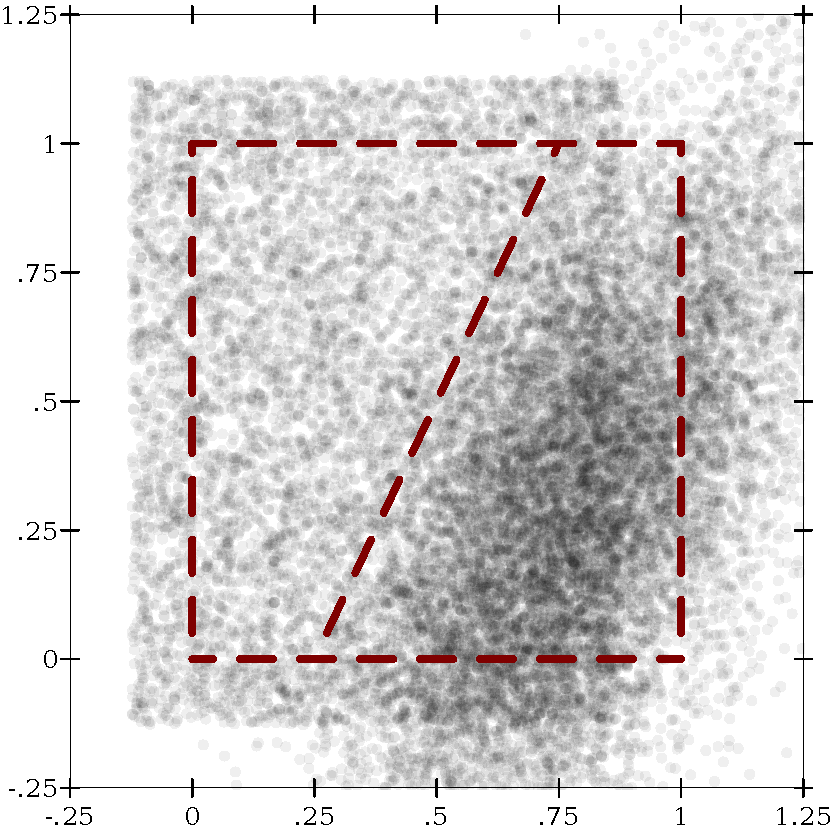
\includegraphics[width=3in]{pimp-sampling-unweighted}
}
\hspace{0.1in}
\subfloat[Resampled by weight]{
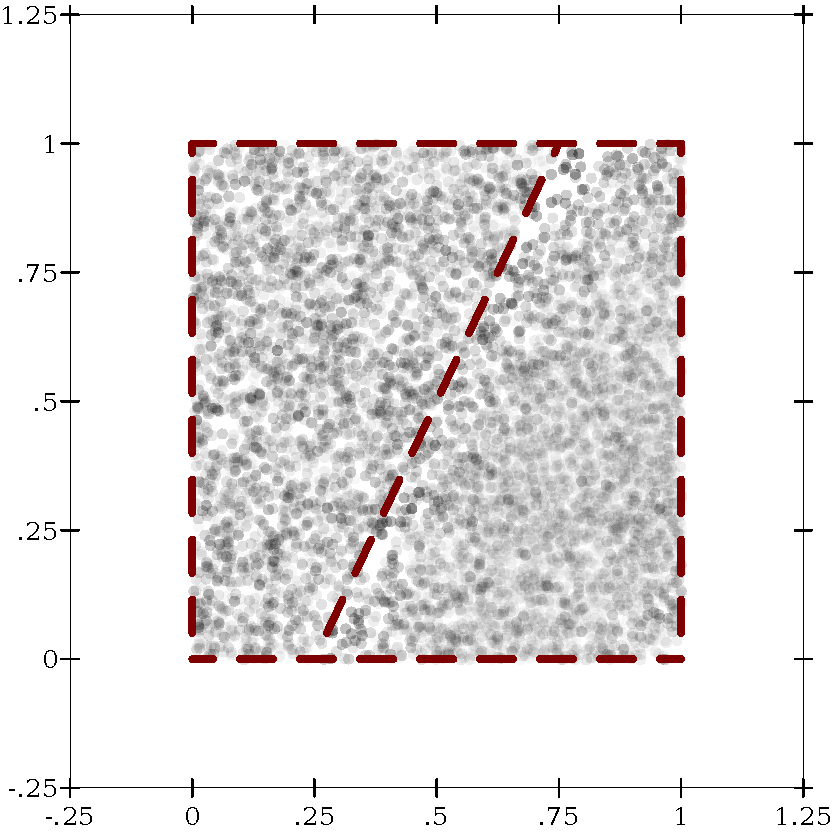
\includegraphics[width=3in]{pimp-sampling-weighted}
}
\caption[ ]{Partitioned importance sampling used to sample uniformly in a partition of the unit square, using two overlapping candidate distributions.}
\label{fig:pimp-sampling-2d}
\end{figure}

\begin{example}[2D partitioned importance sampling]
\figref{fig:pimp-sampling-2d} shows the result of partitioned importance sampling in a partition of the unit square.
In this instance,
\begin{itemize}
	\item $X := [0,1] \times [0,1]$ and $P$ is the uniform measure on $X$ (i.e. area).
	\item $N := \set{left,right}$.
	\item $p := [left \mapsto 0.4, right \mapsto 0.6]$.
	\item $s~left = \setb{\pair{x,y} \in X}{y > 2 \cdot x - \frac{1}{2}}$, similarly for $s~right$.
	\item $Q~left$ is the uniform measure on a superset of $s~left$, and $Q~right$ is a multivariate Gaussian measure centered at $\pair{0.8,0.3}$.
\end{itemize}
The implementation does not actually construct most of these objects. It constructs
\begin{itemize}
	\item A density function $f : \Re \times \Re \tto [0,+\infty)$ to represent $P$.
	\item A family of predicates $s? : N \tto X \tto Bool$ to decide $a \in s~n$.
	\item Candidate densities $g : N \tto X \tto [0,+\infty)$ to represent $Q$.
\end{itemize}
It computes weights using $diff^+~(subcond~P~(s~n))~(Q~n)~a\ =\ f~a~{/}~g~n~a$ when $s?~n~a = true$.
It directly represents only $N$ and $p$, but we will find even this to be infeasible shortly.
\exampleqed
\end{example}

Two properties make the preceeding example simple.
First, the partition has finitely many parts.
Second, the measures $subcond~P~(s~n)$ and $Q~n$ have densities with respect to the same base measure, which ensures $diff^+~(subcond~P~(s~n))~(Q~n)$ exists and is easy to compute.

When sampling in the domain of programs, neither property holds in general.

\subsection{Partitioning Probabilistic Program Domains}

For the random source part $R := J \to [0,1]$ of probabilistic language domains, which consists of infinite binary trees of reals, it is not clear that Theorem~\ref{thm:partitioned-importance-sampling-correctness} is applicable.
The main problem is that infinite-dimensional Radon-Nikod\'ym derivatives do not generally exist.

Fortunately, they \emph{can} exist if the two measures differ in only finitely many axes.
More precisely, let $P_1 : Set~R \to [0,1]$ and $P_2 : Set~R \to [0,1]$ be probability measures, and $J' \subseteq J$ be a finite set of tree indexes.
Suppose $P_1$ can be factored into a distribution $P_1'$ over $J' \to [0,1]$ and a distribution over $(J \w J') \to [0,1]$, and $P_2'$ can be similarly factored into $P_2'$ and \emph{the same} distribution over $(J \w J') \to [0,1]$.
Then, under reasonable conditions (which are analogous to the support of $P_1'$ being no larger than that of  $P_2'$), $diff^+~P_1~P_2$ exists and can be computed using $diff^+~P_1'~P_2'$.
Chapter~\ref{ch:sampling-algorithm-proofs} contains a formal statement of this fact and a proof.

To ensure $subcond~P~(s~n)$ and $Q~n$ differ in only finitely many axes, we partition $R$ according to branch traces.
Each branch trace corresponds with a program that reads any $r \in R$ at only finitely many indexes $J' \subseteq J$.
[XXX: connect idea better]

In the remainder of this subsection, assume a fixed program $\mathit{p}$. Let $f := \meaningofconv{\mathit{p}}_\pbot : \pair{\pair{R,T},\pair{}} \pbotto Y$ be its interpretation as a bottom* arrow computation, with maximal domain $A^*$.
Define $T^* := image~(fst~\arrowcomp~snd)~A^*$ as its \mykeyword{maximal branch trace set} and
$R^* := image~(fst~\arrowcomp~fst)~A^*$ as its \mykeyword{maximal random source set}.

We need a notion of the random sources that agree with a given branch trace $t \in T$; i.e. those $r \in R$ for which $f~\pair{\pair{r,t},\pair{}} \neq \bot$.

\begin{definition}[induced random sources]
\label{def:induced-random-sources}
Let $t \in T$ be a branch trace. The \mykeyword{random sources induced by $t$} are a subset of $R$ defined by
$R' := \setb{r \in R}{\pair{\pair{r,t},\pair{}} \in A^*}$.
%\begin{equation}
	%image~(fst~\arrowcomp~fst)~(preimage~(g~((R \times \set{t}) \times X))~Y)
%\end{equation}
\end{definition}

[XXX: graph of induced partition from program $if~(random < random)~true~false$?]

Using $T$ as the partition index set and defining the partition's parts as induced random sources \emph{almost} works, in the sense that the required Radon-Nikod\'ym derivatives exist.
Unfortunately, we cannot use $T$ or $T^*$ as the partition index set because many branch traces can induce the same random sources.

\begin{example}
For the program
\begin{equation}
	if~(random < p)~0~random
\end{equation}
there are at least two branch traces in the program's maximal domain: $t_0 := [j_0 \mapsto true, * \mapsto \bot]$ and $t_1 := [j_0 \mapsto false, * \mapsto \bot]$.
There is also $[j_0 \mapsto false, left~j_0 \mapsto true, * \mapsto \bot]$, because it agrees with every execution that $[j_0 \mapsto false, * \mapsto \bot]$ agrees with.
In fact, there are infinitely many branch traces in $T^*$ that induce the same random sources as either $t_0$ or $t_1$.
[XXX: tree diagrams?]
\exampleqed
\end{example}

We need to find a subset of branch traces whose induced random sources are disjoint.
The main idea is to define equivalence classes of branch traces that induce the same random sources, and use the ``smallest'' branch trace in each class as a part index.

First, we need to be sure that such equivalence classes can induce a partition.

\begin{theorem}
Let $t_1,t_2 \in T^*$.
If $t_1$ induces $R_1'$ and $t_2$ induces $R_2'$, then $R_1' = R_2'$ or $R_1' \i R_2' = \emptyset$.
\end{theorem}
\begin{proof}
XXX: do this
\end{proof}

To identify the ``smallest'' trace in each class, we must define an ordering over them.
One fairly natural way is to say a branch trace is smaller than another when it describes fewer branch decisions; i.e. its tree has fewer non-$\bot$ elements.
Two branch traces that differ by returning respectively $true$ and $false$ for the same $j$ may represent different execution paths, so they must be incomparable.

\begin{definition}[brach trace partial order]
$t_1 \leq t_2$ when for all $j \in J$, if $t_1~j \neq t_2~j$, then $t_1~j = \bot$.
\end{definition}

If $T^*$ is partitioned into equivalence classes of traces that induce the same random sources, each part in the partition contains a least member with respect to $(\leq)$.

\begin{theorem}
Let $t \in T^*$ induce $R'$, and let $T'$ be the largest subset of $T^*$ that induces $R'$.
$T'$ has a least member $t_*$.
\end{theorem}
\begin{proof}
Define $t_* \in T$ by
\begin{equation}
	t_*\ :=\ \lzfccond{
		\Forall{t' \in T'} t'~j = true & true \\
		\Forall{t' \in T'} t'~j = false & false \\
		else & \bot}
\end{equation}
Thus, $t_* \leq t'$ for all $t' \in T'$, or $t_*$ is a lower bound for $T'$.

Let $r \in R'$.
By construction, every conditional subcomputation at index $j \in J$ agrees with $t_*~j$.
Therefore $f~\pair{\pair{r,t_*},\pair{}} \neq \bot$, so $\pair{\pair{r,t_*},\pair{}} \in A^*$, and thus $t_* \in T'$.
\end{proof}

An easy consequence is $T' = \setb{t' \in T^*}{t_* \leq t'}$. [XXX: is it easy?]
Thus, each least member represents a set of larger branch traces that induce the same set of random sources.

We can get our sought-after index set by defining the set of smallest branch traces.

\begin{definition}[minimal branch traces]
The set of \mykeyword{minimal branch traces} $T_*$ is the set of minimal elements in $T^*$, or
\begin{equation}
	T_*\ :=\ \setb{t_1 \in T^*}{\Forall{t_2 \in T^*} t_2 \leq t_1 \implies t_2 = t_1}
\end{equation}
\end{definition}

\begin{theorem}
\label{thm:minimal-induces-partition}
$T_*$ induces a partition of $R^*$.
\end{theorem}
\begin{proof}
XXX: todo
\end{proof}

We can infer from Theorem~\ref{thm:minimal-induces-partition} that a program's minimal branch trace set $T_*$ contains only the actual branches taken when running the program on every $r \in R^*$.
Therefore, one way to sample from $T_*$ with the correct probability---at least, for programs that halt with probability $1$---would be to choose an $r \in R$ uniformly, and run the program on $r$ while recording each branch decision.

But this sampling scheme has problems similar to those of partitioned sampling (Definition~\ref{def:partitioned-sampling}).
First, it assumes the probabilities of branch traces, which are the probabilities of the $R^*$ subsets they induce, are easy to compute.
Second, we are interested in sampling from an \emph{arbitrarily low-probability subset} of $R^*$, which may be covered by the partition induced by an \emph{arbitrarily low-probability subset} of $T_*$.

It appears we have a chicken-and-egg problem, in that
\begin{enumerate}
	\item Sampling in a small subset of $R^*$ requires sampling in a small subset of $T_*$.
	\item Sampling in a small subset of $T_*$ requires sampling in a small subset of $R^*$.
\end{enumerate}
Fortunately, if we allow ourselves subsets of a slightly larger set than $T_*$, and allow ourselves to sample within overapproximating \emph{covers} of $R^*$ subsets, we can use approximate preimage computation to sample from $T_*$ and $R^*$ subsets simultaneously.

\subsection{Approximate Partitions of Probabilistic Program Domains}

We first define the set of branch traces that is slightly larger than $T_*$.

The idea is to define a set of \emph{feasible} branch traces $T_+$ that is derived only from the \emph{shape} of a program, not its actual executions.
We must then ensure that every additional branch trace (i.e. every $t \in T_+ \w T_*$) induces $\emptyset$, so that $T_+$ induces a partition.
After that, we define an algorithm for sampling from $T_+$, which does not require running a probabilistic program on any $r \in R$, and prove the algorithm correct.
We can then extend this algorithm to use preimage computation to sample in arbitrarily good approximations of small subsets of $T_*$ and $R^*$.

\begin{figure*}[!tb]\centering
\smallmathfont
\subfloat[Branch index arrow. Computations return a lazy tree of type $Idxs$, of feasible branch decisions, ignoring the actual values of $if$ conditions. The arrow is directly implementable in any $\lambda$-calculus.]{
\begin{minipage}{0.98\textwidth}
\begin{align*}
\begin{aligned}[t]
	&\begin{aligned}[t]
		Idxs \ ::= &\ \pair{} \gor \pair{Idxs,Idxs} \\
					&\gor if!idxs~J~(1 \tto Idxs)~(1 \tto Idxs) \\
	\end{aligned} \\
\\[-6pt]
	&\begin{aligned}[t]
		&\arrowarr\pbi : (x \tto y) \tto (J \tto Idxs) \\
		&\arrowarr\pbi~f~j\ :=\ \pair{}
	\end{aligned} \\
\\[-6pt]
	&\begin{aligned}[t]
		&(\arrowcomp\pbi) : (J \tto Idxs) \tto (J \tto Idxs) \tto (J \tto Idxs) \\
		&(k_1~\arrowcomp\pbi~k_2)~j \ :=\ \pair{k_1~(left~j), k_2~(right~j)}
	\end{aligned} \\
\\[-6pt]
	&\begin{aligned}[t]
		&(\arrowpair\pbi) : (J \tto Idxs) \tto (J \tto Idxs) \tto (J \tto Idxs) \\
		&(k_1~\arrowcomp\pbi~k_2)~j \ :=\ \pair{k_1~(left~j), k_2~(right~j)}
	\end{aligned} \\
\end{aligned}
&\tab\tab\tab
\begin{aligned}[t]
	&\begin{aligned}[t]
		&\arrowif\pbi : (J \tto Idxs) \tto (J \tto Idxs) \tto (J \tto Idxs) \tto (J \tto Idxs) \\
		&\arrowif\pbi~k_1~k_2~k_3~j \ := \ 
			\lzfclet{
				idxs_2 & \fun{0} k_2~(left~(right~j)) \\
				idxs_3 & \fun{0} k_3~(right~(right~j))
			}{\pair{k_1~j, if!idxs~j~idxs_2~idxs_3}}
	\end{aligned} \\
\\[-6pt]
	&\begin{aligned}[t]
		&\arrowlazy\pbi : (1 \tto (J \tto Idxs)) \tto (J \tto Idxs) \\
		&\arrowlazy\pbi~k~j \ := \ k~0~j
	\end{aligned} \\
\\[-6pt]
	&\begin{aligned}[t]
		&random\pbi : J \tto Idxs \\
		&random\pbi~j \ := \ \pair{}
	\end{aligned} \\
\end{aligned}
\end{align*}
\vspace{3pt}
\hrule
\end{minipage}
\label{fig:collecting-semantics:arrow}
}

\subfloat[The $\lzfclang$ function $traces$ turns a lazy tree of feasible branch decisions into a set of feasible branch traces.]{
\begin{minipage}{0.98\textwidth}
\begin{equation}
\begin{aligned}
	&traces : Idxs \tto Set~T
\\
	&traces~idxs\ :=\ \U_{n \in \Nat} traces^*~n~idxs~[* \mapsto \bot]
\\[6pt]
	&traces^* : \Nat \tto Idxs \tto T \tto Set~T
\\
	&\lzfcsplit[@{}l@{}l@{}]{
	&traces^*~n~\pair{}~t&\ :=\ \set{t}
\\
	&traces^*~n~\pair{idxs_1,idxs_2}~t&\ :=\ 
		\lzfclet{
			T' & traces^*~n~idxs_1~t
		}{\U_{t' \in T'} traces^*~n~idxs_2~t'}
\\
	&traces^*~0~(if!idxs~j~idxs_2~idxs_3)~t&\ :=\ \set{t}
\\
	&traces^*~n~(if!idxs~j~idxs_2~idxs_3)~t&\ :=\ 
		\lzfcsplit{
			&traces^*~(n-1)~(idxs_2~0)~t[j \mapsto true]\ \u \\
			&traces^*~(n-1)~(idxs_3~0)~t[j \mapsto false]\ \u \\
			&\set{t}}
	}
\end{aligned}
\end{equation}
\vspace{3pt}
\hrule
\end{minipage}
\label{fig:collecting-semantics:traces}
}

\subfloat[The stochastic function $sample!trace$ samples $t$ from the set returned by $traces$, and returns $t$ and its probability. It is directly implementable in any $\lambda$-calculus with probabilistic choice.]{
\begin{minipage}{0.98\textwidth}
\begin{equation}
\begin{aligned}
	&sample!trace : Idxs \to \pair{\Re,T}
\\
	&sample!trace~idxs\ :=\ sample!trace^*~idxs~\pair{1,[* \mapsto \bot]}
\\[6pt]
	&sample!trace^* : Idxs \tto \pair{\Re,T} \tto \pair{\Re,T}
\\
	&\lzfcsplit[@{}l@{}l@{}]{
		&sample!trace^*~\pair{}~pt &\ :=\ pt
\\
		&sample!trace^*~\pair{idxs_1,idxs_2}~pt &\ :=\ 
			\lzfclet{
				pt' & sample!trace^*~idxs_1~pt
			}{sample!trace^*~idxs_2~pt'}
\\
		&sample!trace^*~(if!idxs~j~idxs_2~idxs_3)~\pair{p_t,t} &\ :=\ 
			\lzfclet{
				\pair{p_b,b} & sample!branch~\set{true,false,\bot} \\
				pt' & \pair{p_t \cdot p_b, t[j \mapsto b]}
			}{\lzfccase{b}{
				true & sample!trace^*~(idxs_2~0)~pt' \\
				false & sample!trace^*~(idxs_3~0)~pt' \\
				\bot & pt'
				}
			}
	}
\end{aligned}
\end{equation}
\vspace{3pt}
\hrule
\end{minipage}
\label{fig:collecting-semantics:sample-trace}
}

\caption[]{Branch index collecting semantics.}
\label{fig:collecting-semantics}
\end{figure*}

Defining $T_+$ in terms of a program's abstract branching shape requires an additional nonstandard interpretation.
\figref{fig:collecting-semantics:arrow} defines the \mykeyword{branch index} arrow.
Its type is $J \tto Idxs$, which does not refer to a domain or codomain type of program values because its computations do not receive or compute program values.
Instead, they build lazy trees of possible branching decisions, ignoring the actual values of $if$ conditions.
For example, lifted, pure functions are interpreted as $\fun{j} \pair{}$, which takes the function's computation index and returns no decisions.
Composition and pairing of subcomputations $k_1$ and $k_2$ both return $\pair{k_1~(left~j),k_2~(right~j)}$: a node with two children that contain the feasible branch decisions in their subcomputations.

Only $ifte\pbi$ does more than simple structural recursion: it returns $if!idxs~j~idxs_2~idxs_3$ to represent a decision at computation index $j$.
The children $idxs_2$ and $idxs_3$ are lazy, abstract representations of the $if$'s branches.
Like a concrete execution, a branch trace sampler is expected to compute and recur through only one of them.

\figref{fig:collecting-semantics:traces} defines the function $traces$, which transforms these lazy trees of type $Idxs$ into sets of branch traces.
To ensure $trace$ always terminates, it is defined using a depth-limited helper function, which it calls with every depth $n \in \Nat$, and collects the results in a countable union.
It is thus unimplementable, but we will use it only to precisely define the range of a random value.

We define a program's feasible branch traces using the standard first-order semantic function $\meaningofconv{\cdot}_a$ with arrow $a = idxs^*$.

\begin{definition}[feasible branch traces]
A program $\mathit{p}$'s \mykeyword{feasible branch traces} are those in the set $T_+ := traces~(\meaningofconv{\mathit{p}}\pbi~j_0)$.
\end{definition}

If we are to sample $t \in T_+$ and then sample within the $R'$ induced by $t$, we must ensure that $T_+$ includes $T_*$ and induces a partition.

\begin{theorem}
Let $t \in T$ induce $R'$. $R' \neq \emptyset$ if and only if $t \in T^*$. [XXX: needed?]
\end{theorem}
\begin{proof}
$R' \neq \emptyset$ if and only if there is an $r \in R'$ such that $\pair{\pair{r,t},\pair{}} \in A^*$.
\end{proof}

\begin{theorem}
For all $t \in T_+$, either $t \in T_*$ or $t$ induces $\emptyset$.
\end{theorem}
\begin{proof}
XXX: todo
\end{proof}

\begin{corollary}
$T_+$ induces a partition of $R^*$.
\end{corollary}

XXX: now we define a stochastic procedure for sampling in $T_+$

XXX: apologize for being less precise (e.g. stochastic procedures look like $\lzfclang$ but aren't; we assume every operation is lifted to receive a random source as input, etc.)

XXX: suppose we have a stochastic procedure $sample!branch : Set~Bool_\bot \tto \pair{\Re,Bool_\bot}$, where $sample!branch~B$ returns any member of $B$ with some nonzero, constant probability

\figref{fig:collecting-semantics:sample-trace} defines $sample!trace$, a stochastic procedure defined in terms of $sample!branch$.
Given an $idxs : Idxs$, it returns a member of $traces~idxs$ and its probability.
In other words, for a program $\mathit{p}$, the probability that $\pair{p_t,t} = sample!trace~(\meaningofconv{\mathit{p}}\pbi~j_0)$ is $p_t$, and $t \in T_+$.
Further, every $t \in T_+$ has a constant, nonzero probability of being chosen.

Of course, we must prove these facts.

XXX: move the following soundness and completeness proofs to Chapter 10, or define $T_+$ in terms of $sample!trace$ to make the proofs unnecessary; whether the latter will work (or whether it will work better) will probably become clear when I do the missing proof above

\begin{theorem}[$sample!trace^*$ soundness]
For all $t \in T$ and $idxs: Idxs$, there exists an $n \in \Nat$ such that $snd~(sample!trace^*~idxs~\pair{p_t,t}) \in traces^*~n~idxs~t$.
\end{theorem}
\begin{proof}
By structural induction on $Idxs$.

Case $idxs = \pair{}$.
For all $n \in \Nat$, these two statements are equivalent by substituting definitions of $sample!trace^*$ and $traces^*$:
\begin{equation}
\begin{aligned}
	snd~(sample!trace^*~\pair{}~\pair{p_t,t}) &\in traces^*~n~\pair{}~t \\
	t &\in \set{t}
\end{aligned}
\end{equation}

Case $idxs = \pair{idxs_1,idxs_2}$.
Let
\begin{equation}
\begin{aligned}
	\pair{p_t',t'}&\ :=\ sample!trace^*~idxs_1~\pair{p_t,t} \\
	\pair{p_t'',t''}&\ :=\ sample!trace^*~idxs_2~\pair{p_t',t'}
\end{aligned}
\end{equation}
as in the definition of $sample!trace^*$.
By hypothesis, there exists an $n' \in \Nat$ such that $t' \in traces^*~n'~idxs_1~t$.
Again by hypothesis, there exists an $n'' \in \Nat$ such that $t'' \in traces^*~n''~idxs_2~t'$.
Let $n := max~n'~n''$.

Case $idxs = if!idxs~j~idxs_2~idxs_3$.
Let
\begin{equation}
\begin{aligned}
	\pair{p_b,b}&\ :=\ sample!branch~\set{true,false,\bot} \\
	pt' &\ :=\ \pair{p_t \cdot p_b, t[j \mapsto b]}
\end{aligned}
\end{equation}
as in the definition of $sample!trace^*$, and let $\pair{p_t',t'}\ =\ pt'$.
If $b = true$, by hypothesis, there exists an $n' \in \Nat$ such that $snd~(sample!trace^*~(idxs_2~0)~pt') \in traces^*~n'~(idxs_2~0)~t'$; similarly for $b = false$. Let $n := n' + 1$, so $n' = n - 1$.
If $b = \bot$, then $t' = t$, and $t \in \set{t}$ for all $n \in \Nat$.
\end{proof}

\begin{corollary}[$sample!trace$ soundness]
For all $idxs : Idxs$, $snd~(sample!trace~idxs) \in traces~idxs$.
\end{corollary}

\begin{theorem}[$sample!trace^*$ completeness]
For all $idxs : Idxs$, $t \in T$ and $n \in \Nat$, $t' \in traces^*~n~idxs~t$ implies $Pr[snd~(sample!trace^*~idxs~\pair{p_t,t}) = t'] > 0$ (or just $Pr[t'] > 0$).
\end{theorem}
\begin{proof}
By structural induction on $Idxs$.

Case $idxs = \pair{}$.
By definition of $traces^*$, $t' \in traces^*~n~\pair{}~t$ if and only if $t' \in \set{t}$, or $t' = t$.
By definition of $sample!trace^*$, $Pr[snd~(sample!trace^*~idxs~\pair{p_t,t}) = t] = 1$.

Case $idxs = \pair{idxs_1,idxs_2}$.
Let
\begin{equation}
\begin{aligned}
	T'&\ :=\ traces^*~n~idxs_1~t \\
	T''&\ :=\ \U_{t' \in T'} traces^*~n~idxs_2~t'
\end{aligned}
\end{equation}
as in the definition of $traces^*$. Let
\begin{equation}
\begin{aligned}
	\pair{p_t',t'}&\ :=\ sample!trace^*~idxs_1~\pair{p_t,t} \\
	\pair{p_t'',t''}&\ :=\ sample!trace^*~idxs_2~\pair{p_t',t'}
\end{aligned}
\end{equation}
as in the definition of $sample!trace^*$.
Suppose $t'' \in T''$.
Then there exists a $t' \in T'$ such that $t'' \in traces^*~n~idxs_2~t'$.
By hypothesis, $Pr[t'] > 0$, therefore by hypothesis, $Pr[t''] > 0$.

Case $idxs = if!idxs~j~idxs_2~idxs_3$.
Let
\begin{equation}
\begin{aligned}
	\pair{p_b,b}&\ :=\ sample!branch~\set{true,false,\bot} \\
	pt' &\ :=\ \pair{p_t \cdot p_b, t[j \mapsto b]}
\end{aligned}
\end{equation}
as in the definition of $sample!trace^*$, and let $\pair{p_t',t'}\ =\ pt'$.

If $n = 0$, then let
\begin{equation}
\begin{aligned}
	T'&\ :=\ traces^*~0~idxs~t = \set{t}
\end{aligned}
\end{equation}
as in the definition of $traces^*$.
Suppose $t' \in T'$, equiv. $t' = t$, so $Pr[t'] > 0$ iff $Pr[t] > 0$.
Because $Pr[b = \bot] > 0$ and $t[j \mapsto \bot] = t$, $Pr[t] > 0$.

If $n > 0$, then expand $traces^*~n~idxs~t$ to
\begin{equation}
\begin{aligned}
	T_{true}'&\ :=\ traces^*~(n-1)~(idxs_2~0)~t[j \mapsto true]
\\
	T_{false}'&\ :=\ traces^*~(n-1)~(idxs_3~0)~t[j \mapsto false]
\\
	T_\bot'&\ :=\ \set{t}
\\
	T'&\ :=\ T_{true}' \u T_{false}' \u T_\bot'
\end{aligned}
\end{equation}
as in the definition of $traces^*$.
Suppose $t' \in T'$.
If $t' \in T_{true}'$, then because $Pr[b = true] > 0$, by hypothesis, $Pr[t'] > 0$; similarly for $t' \in T_{false}'$ and $t' \in T_\bot'$.
\end{proof}

\begin{corollary}[$sample!trace$ completeness]
For all $idxs : Indx$, $t \in traces~idxs$ implies $Pr[snd~(sample!trace~idxs) = t] > 0$.
\end{corollary}

\begin{theorem}[$sample!trace^*$ correctness]
Let $idxs : Idxs$, $t \in T_+$, $p_t \in [0,1]$, and $\pair{p_t',t'} := sample!trace^*~idxs~\pair{p_t,t}$.
If $Pr[t] = p_t$, then $Pr[t'] = p_t'$.
\end{theorem}
\begin{proof}
By structural induction on $Idxs$.

Case $idxs = \pair{}$.
By definition of $sample!trace^*$, $\pair{p_t',t'} = \pair{p_t,t}$.
Clearly $Pr[t] = p_t$ implies $Pr[t'] = p_t'$.

Case $idxs = \pair{idxs_1,idxs_2}$.
Let
\begin{equation}
\begin{aligned}
	\pair{p_t',t'}&\ :=\ sample!trace^*~idxs_1~\pair{p_t,t} \\
	\pair{p_t'',t''}&\ :=\ sample!trace^*~idxs_2~\pair{p_t',t'}
\end{aligned}
\end{equation}
as in the definition of $sample!trace^*$.
By hypothesis, $Pr[t] = p_t$ implies $Pr[t'] = p_t'$, which (by hypothesis) implies $Pr[t''] = p_t''$.

Case $idxs = if!idxs~j~idxs_2~idxs_3$.
Let
\begin{equation}
\begin{aligned}
	\pair{p_b,b}&\ :=\ sample!branch~\set{true,false,\bot} \\
	pt' &\ :=\ \pair{p_t \cdot p_b, t[j \mapsto b]}
\end{aligned}
\end{equation}
as in the definition of $sample!trace^*$, and let $\pair{p_t',t'}\ =\ pt'$.
By definition of $sample!branch$, $Pr[b] = p_b$.
Because $b$ and $t$ are independently chosen and $t'$ can be generated by no other execution path, $Pr[t'] = Pr[t] \cdot Pr[b] = p_t \cdot p_b$.
If $b = true$, then in $\pair{p_t'',t''} := sample!trace^*~(idxs_2~0)~pr'$, by hypothesis, $Pr[t''] = p_t''$; similarly for $b = false$.
\end{proof}

\begin{corollary}[$sample!trace$ correctness]
If $\pair{p_t,t} := sample!trace~idxs$, then $Pr[t] = p_t$.
\end{corollary}

XXX: sampling from a \emph{subset} of $T_+$ that induces a part of the partition of $R^*$:
\begin{equation}
\begin{aligned}
	&sample!part : Idxs \tto \pair{\Re,Rect~\pair{R,T}} \tto \pair{\Re,Rect~\pair{R,T}} \\
	&\lzfcsplit{
	&sample!part~idxs~\pair{p,R \times T}\ := \\
	&\tab
	\lzfccase{\pair{idxs, \pair{p, refine~(R \times T)}}}{
		\pair{\pair{}, pr} & pr
\\
		\pair{\pair{idxs_1,idxs_2}, pr} &
			\lzfclet{
				pr' & sample!part~idxs_1~pr
			}{sample!part~idxs_2~pr'}
\\
		\pair{if!idxs~j~idxs_2~idxs_3, \pair{p,R \times T}} &
			\lzfclet{
				\pair{p_b,b} & sample!branch~(proj~j~T) \\
				pr' & \pair{p \cdot p_b, R \times unproj~j~T~\set{b}}
			}{\lzfccase{b}{
				true & sample!part~(idxs_2~0)~pr' \\
				false & sample!part~(idxs_3~0)~pr' \\
				\bot & \pair{p \cdot p_b,\emptyset}
				}
			}
	}
	}
\end{aligned}
\end{equation}

XXX: sampling a weighted point from $Rect~\pair{R,T}$:
\begin{equation}
\begin{aligned}
			\lzfclet{
				\pair{r,q} & sample!point~R \\
				t & \The{t \in T} \Forall{t' \in T} t \leq t' \\
				b & f~\pair{\pair{r,t},\pair{}} \\
				w & if~(b \in B)~(1~{/}~p \cdot 1~{/}~q)~0
			}{\pair{r,w}}
\end{aligned}
\end{equation}

XXX: the least $t \in T$, or $\The{t \in T} \Forall{t' \in T} t \leq t'$, is easy to compute: set each unrestricted axis to $\bot$

XXX: decide what theorems are needed and prove them

XXX: extension: interval splitting

XXX: extension: sampling a weighted point using refinement

XXX: extension: not sampling any decision as $\bot$ when sampling in $T_+$; characterize the programs for which this extension doesn't terminate; explain options to detect or fix

\mathversion{normal}



\chapter{Measurability}
\label{ch:measurability}

\mathversion{sans}

Proving measurability is critical in proving correctness, in that it establishes that the outputs of all programs have sensible distributions.
While critical, it is somewhat distracting to the main narrative.
Instead of ignoring measurability, however, as is so often done, we have moved it to the end, where readers who are somehow \emph{still starving for even more mathematics} can devour it and---possibly---finally be satiated.

Unsatiated readers may afterward proceed to Appendix~\ref{ch:sampling-algorithm-proofs}.

\section{Basic Definitions}

For readers familiar with topology, we review the necessary fundamentals by analogy to topology.
However, we have tried to include enough of the fundamentals~\cite{cit:klenke-2006-probability} that readers not familiar with basic topology can verify the proofs.

The analogue of a topology of open sets is a $\sigma$-algebra of measurable sets.

\begin{definition}[$\sigma$-algebra, measurable set]
A collection of sets $\A \subseteq \powerset~X$ is called a \keyword{$\sigma$-algebra} on $X$ if it contains $X$ and is closed under complements and countable unions.
The sets in $\A$ are called \keyword{measurable sets}.
\end{definition}

$X \w X = \emptyset$, so $\emptyset \in \A$.
Additionally, it follows from De Morgan's law that $\A$ is closed under countable intersections.

The analogue of continuity is measurability.

\begin{definition}[measurable mapping]
Let $\A$ and $\B$ be $\sigma$-algebras on $X$ and $Y$.
A mapping $g : X \pto Y$ is $\A!\B$-\keyword{measurable} if for all $B \in \B$, $preimage~g~B \in \A$.
\end{definition}

When the domain and codomain $\sigma$-algebras $\A$ and $\B$ are clear from context, we will simply say $g$ is \keyword{measurable}.

Measurability is usually a weaker condition than continuity.
For example, with respect to the $\sigma$-algebra generated from $\Re$'s standard topology (i.e. using the standard topology as a sort of ``base''), measurable $\Re \pto \Re$ functions may have countably many discontinuities.
Likewise, real comparison functions such as $(=)$, $(<)$, $(>)$ and their negations are measurable, but not continuous.

Product $\sigma$-algebras are defined analogously to product topologies.

\begin{definition}[finite product $\sigma$-algebra]
\label{def:finite-product-sigma-algebra}
Let $\A_1$ and $\A_2$ be $\sigma$-algebras on $X_1$ and $X_2$, and define $X := X_1 \times X_2$.
The \keyword{product $\sigma$-algebra} $\A_1 \otimes \A_2$ is the smallest (i.e. coarsest) $\sigma$-algebra for which $mapping~fst~X$ and $mapping~snd~X$ are measurable.%
\end{definition}

\begin{definition}[arbitrary product $\sigma$-algebra]
\label{def:arbitrary-product-sigma-algebra}
Let $\A$ be a $\sigma$-algebra on $X$.
The \keyword{product $\sigma$-algebra} $\A^{\otimes J}$ is the smallest $\sigma$-algebra for which, for all $j \in J$, $mapping~(\pi~j)~(J \to X)$ is measurable.%
\end{definition}

\section{Measurable Pure Computations}

It is easier to prove measurability of pure computations than to prove measurability of partial, probabilistic ones.
Further, we can use the results to prove that the interpretations of all partial, probabilistic expressions are measurable.

We must first define what it means for a \emph{computation} to be measurable.

\begin{definition}[measurable mapping arrow computation]
\label{def:measurable-mapping-arrow-computation}
Let $\A$ and $\B$ be $\sigma$-algebras on $X$ and $Y$.
A computation $g : X \mapto Y$ is $\A!\B$-\keyword{measurable} if $g~A^*$ is an $\A!\B$-measurable mapping, where $A^*$ is $g$'s maximal domain.%
\end{definition}

\begin{theorem}[maximal domain measurability]
Let $g : X \mapto Y$ be an $\A!\B$-measurable mapping arrow computation.
Its maximal domain $A^*$ is in $\A$.
\end{theorem}
\begin{proof}
Because $g~A^*$ is measurable, $preimage~(g~A^*)~Y = A^*$ is in $\A$.
\end{proof}

Mapping arrow computations can be applied to sets other than their maximal domains.
We need to ensure doing so yields a measurable mapping, at least for measurable subsets of $A^*$.
Fortunately, that is true without any extra conditions.

\begin{lemma}
\label{lem:restricted-mappings-are-measurable}
Let $g : X \pto Y$ be an $\A!\B$-measurable mapping.
For any $A \in \A$, $restrict~g~A$ is $\A!\B$-measurable.%
\end{lemma}

\begin{theorem}
\label{thm:restricted-computations-are-measurable}
Let $g : X \mapto Y$ be an $\A!\B$-measurable mapping arrow computation with maximal domain $A^*$.
For all $A \subseteq A^*$ with $A \in \A$, $g~A$ is $\A!\B$-measurable.
\end{theorem}
\begin{proof}
By Theorem~\ref{thm:mapping-arrow-restriction} (mapping arrow restriction) and Lemma~\ref{lem:restricted-mappings-are-measurable}.
\end{proof}

We do not need to prove all interpretations using $\meaningof{\cdot}\gen$ are measurable.
However, we do need to prove mapping arrow combinators preserve measurability.

\subsection{Composition}
Proving compositions are measurable takes the most work.
The main complication is that, under measurable mappings, while \emph{preimages} of measurable sets are measurable, \emph{images} of measurable sets may not be.
We need the following four extra theorems to get around this.

\begin{lemma}[images of preimages]
\label{lem:images-of-preimages}
If $g : X \pto Y$ and $B \subseteq Y$, $image~g~(preimage~g~B) \subseteq B$.%
\end{lemma}

\begin{lemma}[expanded post-composition]
\label{lem:composition-expansion}
Let $g_1 : X \pto Y$ and $g_2 : Y \pto Z$ such that $range~g_1 \subseteq domain~g_2$, and let $g_2' : Y \pto Z$ such that $g_2 \subseteq g_2'$.
Then $g_2 \circ\map g_1 = g_2' \circ\map g_1$.%
\end{lemma}

\begin{theorem}[mapping arrow monotonicity]
\label{thm:mapping-arrow-monotonicity}
Let $g : X \mapto Y$.
For any $A' \subseteq A \subseteq A^*$, $g~A' \subseteq g~A$.%
\end{theorem}
\begin{proof}
By Theorem~\ref{thm:mapping-arrow-restriction} (mapping arrow restriction).
\end{proof}

\begin{theorem}[maximal domain subsets]
\label{thm:maximal-domain-subsets}
Let $g : X \mapto Y$. For all $A \subseteq A^*$, $domain~(g~A) = A$.%
\end{theorem}
\begin{proof}
Follows from Theorem~\ref{thm:domain-closure-operators}.
\end{proof}

Now we can prove measurability.

\begin{lemma}[$(\circ\map)$ measurability]
\label{lem:compositions-are-measurable}
If $g_1 : X \pto Y$ is $\A!\B$-measurable and $g_2 : Y \pto Z$ is $\B!\C$-measurable, then $g_2 \circ\map g_1$ is $\A!\C$-measurable.%
\end{lemma}

\begin{theorem}[$(\compmap)$ measurability]
If $g_1 : X \mapto Y$ is $\A!\B$-measurable and $g_2 : Y \mapto Z$ is $\B!\C$-measurable, then $g_1~\compmap~g_2$ is $\A!\C$-measurable.
\end{theorem}
\begin{proof}
Let $A^* \in \A$ and $B^* \in \B$ be respectively $g_1$'s and $g_2$'s maximal domains.
The maximal domain of $g_1~\compmap~g_2$ is $A^{**} := preimage~(g_1~A^*)~B^*$, which is in $\A$.
By definition,
\begin{equation}
	(g_1~\compmap~g_2)~A^{**} \ = \ 
		\lzfclet{
			g_1' & g_1~A^{**} \\
			g_2' & g_2~(range~g_1')
		}{g_2' \circ\map g_1'}
\end{equation}
By Theorem~\ref{thm:restricted-computations-are-measurable}, $g_1'$ is an $\A!\B$-measurable mapping.
Unfortunately, $g_2'$ may not be $\B!\C$-measurable when $range~g_1' \not\in \B$.

Let $g_2'' := g_2~B^*$, which is a $\B!\C$-measurable mapping.
By Lemma~\ref{lem:compositions-are-measurable}, $g_2'' \circ\map g_1'$ is $\A!\C$-measurable.
We need only show that $g_2' \circ\map g_1' = g_2'' \circ\map g_1'$, which by Lemma~\ref{lem:composition-expansion} is true if $range~g_1' \subseteq domain~g_2'$ and $g_2' \subseteq g_2''$.

By Theorem~\ref{thm:maximal-domain-subsets}, $A^{**} \subseteq A^*$ implies $domain~g_1' = A^{**}$.
By Theorem~\ref{thm:mapping-arrow-monotonicity} and Lemma~\ref{lem:images-of-preimages},
\begin{align*}
\numberthis
	range~g_1'
		%&\ =\ image~g_1'~A^{**} \\
		&\ =\ image~(g_1~A^{**})~(preimage~(g_1~A^*)~B^*) \\
		&\ =\ image~(g_1~A^*)~(preimage~(g_1~A^*)~B^*) \\
		&\ \subseteq\ B^*
\end{align*}
$range~g_1' \subseteq B^*$ implies (by Theorem~\ref{thm:maximal-domain-subsets}) that $domain~g_2' = range~g_1'$, and (by Theorem~\ref{thm:mapping-arrow-monotonicity}) that $g_2' \subseteq g_2''$.
\end{proof}

\subsection{Pairing}
Proving pairing preserves measurability is straightforward given a corresponding theorem about mappings.

\begin{lemma}[$\pair{\cdot,\cdot}\map$ measurability]
\label{lem:pairings-are-measurable}
If $g_1 : X \pto Y_1$ is $\A!\B_1$-measurable and $g_2 : X \pto Y_2$ is $\A!\B_2$-measurable, then $\pair{g_1,g_2}\map$ is $\A!(\B_1 \otimes \B_2)$-measurable.%
\end{lemma}

\begin{theorem}[$(\pairmap)$ measurability]
If $g_1 : X \mapto Y_1$ is $\A!\B_1$-measurable and $g_2 : X \mapto Y_2$ is $\A!\B_2$-measurable, then $g_1~\pairmap~g_2$ is $\A!(\B_1 \otimes \B_2)$-measurable.
\end{theorem}
\begin{proof}
Let $A_1^*$ and $A_2^*$ be respectively $g_1$'s and $g_2$'s maximal domains.
The maximal domain of $g_1~\pairmap~g_2$ is $A^{**} := A_1^* \i A_2^*$, which is in $\A$.
By definition, $(g_1~\pairmap~g_2)~A^{**} = \pair{g_1~A^{**},g_2~A^{**}}\map$, which by Lemma~\ref{lem:pairings-are-measurable} is $\A!(\B_1 \otimes \B_2)$-measurable.
\end{proof}

\subsection{Conditional}
Conditionals can be proved measurable given a theorem that ensures the measurability of \emph{finite} unions of disjoint, measurable mappings.
We will need the corresponding theorem for \emph{countable} unions further on, however.

\begin{lemma}[union of measurable mappings]
\label{lem:union-of-measurable-mappings}
The union of a countable set of $\A!\B$-measurable mappings with disjoint domains is $\A!\B$-measurable.%
\end{lemma}

\begin{theorem}[$\ifmap$ measurability]
If $g_1 : X \mapto Bool$, and $g_2 : X \mapto Y$ and $g_3 : X \mapto Y$ are respectively $\A!(\powerset~Bool)$-measurable and $\A!\B$-measurable, then $\ifmap~g_1~g_2~g_3$ is $\A!\B$-measurable.
\end{theorem}
\begin{proof}
Let $\A_1^*$, $\A_2^*$ and $\A_3^*$ be $g_1$'s, $g_2$'s and $g_3$'s maximal domains.
The maximal domain of $\ifmap~g_1~g_2~g_3$ is $A^{**}$, defined by
\begin{equation}
\begin{aligned}
	A_2^{**} &\ :=\ A_2^* \i preimage~(g_1~\A_1^*)~\set{true} \\
	A_3^{**} &\ :=\ A_3^* \i preimage~(g_1~\A_1^*)~\set{false} \\
	A^{**} &\ :=\ A_2^{**} \uplus A_3^{**}
\end{aligned}
\end{equation}
Because $preimage~(g_1~\A_1^*)~B \in \A$ for any $B \subseteq Bool$, $A^{**} \in \A$.
By definition,
\begin{equation}
	\ifmap~g_1~g_2~g_3~A^{**} \ = \ 
		\lzfclet{
			g_1' & g_1~A^{**} \\
			g_2' & g_2~(preimage~g_1'~\set{true}) \\
			g_3' & g_3~(preimage~g_1'~\set{false})
		}{g_2' \uplus\map g_3'}
\end{equation}
By hypothesis, $g_1'$, $g_2'$ and $g_3'$ are measurable mappings.
By Theorem~\ref{thm:mapping-arrow-restriction} (mapping arrow restriction), $g_2'$ and $g_3'$ have disjoint domains.
Apply Lemma~\ref{lem:union-of-measurable-mappings}.
\end{proof}

\subsection{Laziness}
We must first prove measurability of an often-ignored corner case.

\begin{theorem}[measurability of $\emptyset$]
\label{thm:empty-mapping-measurable}
For any $\sigma$-algebras $\A$ and $\B$, the empty mapping $\emptyset$ is $\A!\B$-measurable.%
\end{theorem}
\begin{proof}
For any $B \in \B$, $preimage~\emptyset~B = \emptyset$, and $\emptyset \in \A$.
\end{proof}

\begin{theorem}[measurability under $\lazymap$]
Let $g : 1 \tto (X \mapto Y)$. If $g~0$ is $\A!\B$-measurable, then $\lazymap~g$ is $\A!\B$-measurable.
\end{theorem}
\begin{proof}
The maximal domain $A^{**}$ of $\lazymap~g$ is that of $g~0$.
By definition,
\begin{equation}
	\lazymap~g~A^{**} \ = \ if~(A^{**} = \emptyset)~\emptyset~(g~0~A^{**})
\end{equation}
If $A^{**} = \emptyset$, then $\lazymap~g~A^{**} = \emptyset$; apply Theorem~\ref{thm:empty-mapping-measurable}.
If $A^{**} \neq \emptyset$, then $\lazymap~g = g~0$, which is $\A!\B$-measurable.
\end{proof}

\section{Measurable Probabilistic Computations}

As with pure computations, we must first define what it means for an effectful computation to be measurable.

\begin{definition}[measurable mapping* arrow computation]
Let $\A$ and $\B$ be $\sigma$-algebras on $(\Omega \times T) \times X$ and $Y$.
A computation $g : X \pmapto Y$ is $\A!\B$-\keyword{measurable} if $g~j_0$ is an $\A!\B$-measurable mapping arrow computation.
\end{definition}

\begin{theorem}
If $g : X \pmapto Y$ is $\A!\B$-measurable, then for all $j \in J$, $g~j$ is an $\A!\B$-measurable mapping arrow computation.
\end{theorem}
\begin{proof}
By induction on $J$: if $g~j$ is measurable, so are $g~(left~j)$ and $g~(right~j)$.
\end{proof}

To make general measurability statements about computations, whether they have flat or product types, it helps to have a notion of a standard $\sigma$-algebra.

\begin{definition}[standard $\sigma$-algebra]
\label{def:standard-sigma-algebra}
For a set $X$ used as a type, $\Sigma~X$ denotes its \mykeyword{standard $\sigma$-algebra}, which must be defined under the following constraints:
\begin{align}
	\Sigma~\pair{X_1,X_2} & = \Sigma~X_1 \otimes \Sigma~X_2
	\label{eqn:standard-finite-product-rule}
\\
	\Sigma~(J \to X) & = (\Sigma~X)^{\otimes J}
	\label{eqn:standard-arbitrary-product-rule}
%\\
%	X' \in \Sigma~X \ \implies \ \Sigma~X' & = \setb{X' \i A}{A \in \Sigma~X}
%	\label{eqn:standard-subset-rule}
\end{align}
\end{definition}

From here on, when no $\sigma$-algebras are given, ``measurable'' means ``measurable with respect to standard $\sigma$-algebras.''

The following definitions allow distinguishing the results of conditional expressions and any two branch traces:
\begin{align}
	\Sigma~Bool &\ ::=\ \powerset~Bool
	\label{eqn:standard-boolean-rule}
\\
	\Sigma~T &\ ::=\ \powerset~T
	\label{eqn:standard-traces-rule}
\end{align}

\begin{lemma}[measurable mapping arrow lifts]
$\arrmap~id$, $\arrmap~fst$ and $\arrmap~snd$ are measurable.
$\arrmap~(const~b)$ is measurable if $\set{b}$ is a measurable set.
For all $j \in J$, $\arrmap~(\pi~j)$ is measurable.
\end{lemma}

%XXX: should that really be a lemma? $\arrmap$ removes $\bot$ from the domain

\begin{corollary}[measurable mapping* arrow lifts]
$\arrpmap~id$, $\arrpmap~fst$ and $\arrpmap~snd$ are measurable.
$\arrpmap~(const~b)$ is measurable if $\set{b}$ is a measurable set.
$random\pmap$ and $branch\pmap$ are measurable.
\end{corollary}

\begin{theorem}[$AStore$ combinators preserve measurability]
\label{thm:astore-measurability-transfer}
Every $AStore$ arrow combinator produces measurable mapping* computations from measurable mapping* computations.%
\end{theorem}
\begin{proof}
$AStore$'s combinators are defined in terms of the base arrow's combinators and $\arrmap~fst$ and $\arrmap~snd$.
\end{proof}

\begin{theorem}[$\convifpmap$ measurability]
$\convifpmap$ is measurable.
\end{theorem}
\begin{proof}
$branch\pmap$ is measurable, and $\arrmap~agrees$ is measurable by~\eqref{eqn:standard-boolean-rule}.
\end{proof}

We can now prove all nonrecursive programs measurable by induction.

\begin{definition}[finite expression]
\label{def:finite-expression}
A \mykeyword{finite expression} is any expression for which no subexpression is a first-order application.%
\end{definition}

\begin{theorem}[all finite expressions are measurable]
\label{thm:nonrecursive-programs-are-measurable}
For all finite expressions $\mathit{e}$, $\meaningof{\mathit{e}}\pmap$ is measurable.%
\end{theorem}
\begin{proof}
By structural induction and the above theorems.
\end{proof}

Now all we need to do is represent recursive programs as a collection of finite expressions interpreted as mappings, and take their union.

\begin{theorem}[approximation with finite expressions]
\label{thm:nonrecursive-approximation}
Let $g := \meaningofconv{\mathit{e}}\pmap : X \pmapto Y$ and $t \in T$.
Define $A := (\Omega \times \set{t}) \times X$.
There is a finite expression $\mathit{e'}$ for which $\meaningof{\mathit{e'}}\pmap~j_0~A = g~j_0~A$.%
\end{theorem}
\begin{proof}
Let the index prefix $J'$ contain every $j$ for which $t~j \neq \bot$.
To construct $\mathit{e'}$, exhaustively apply first-order functions in $\mathit{e}$, but replace any $\convifpmap$ whose index $j$ is not in $J'$ with the equivalent expression $\bot$.
Because $\mathit{e}$ is well-defined, recurrences must be guarded by $if$, so this process terminates after finitely many first-order applications.
\end{proof}

\begin{theorem}[all probabilistic expressions are measurable]
\label{thm:everything-is-measurable}
For all expressions $\mathit{e}$, $\meaningofconv{\mathit{e}}\pmap$ is measurable.%
\end{theorem}
\begin{proof}
Let $g := \meaningofconv{\mathit{e}}\pmap$ and $g' := g~j_0~((\Omega \times T) \times X)$.
By Corollary~\ref{cor:correct-convergence} (correct computation everywhere), $g' = g~j_0~A^*$ where $A^*$ is $g$'s maximal domain; thus we need only show $g'$ is a measurable mapping.

By Theorem~\ref{thm:mapping-arrow-restriction} (mapping arrow restriction),
\begin{equation}
	g' \ =\ \bigcup\limits_{t \in T} g~j_0~((\Omega \times \set{t}) \times X)
\end{equation}
By Theorem~\ref{thm:nonrecursive-approximation} (approximation with finite expressions), for every $t \in T$, there is a finite expression whose interpretation agrees with $g$ on $(\Omega \times \set{t}) \times X$.
Therefore, by Theorem~\ref{thm:nonrecursive-programs-are-measurable} (all finite expressions are measurable), $g~j_0~((\Omega \times \set{t}) \times X)$ is a measurable mapping.
By Theorem~\ref{thm:mapping-arrow-restriction} (mapping arrow restriction), they have disjoint domains.
By Lemma~\ref{lem:union-of-measurable-mappings} (union of measurable mappings), their union is measurable.
\end{proof}

Theorem~\ref{thm:everything-is-measurable} remains true when $\meaningof{\cdot}\pmap$ is extended with any rule whose right side is measurable, including rules for real arithmetic, equality, inequality and limits.
More generally, any continuous or (countably) piecewise continuous function can be made available as a language primitive, as long as its domain's and codomain's standard $\sigma$-algebras are generated from their topologies.

$\meaningof{\cdot}\pmap$ may be composed with another semantic function that defunctionalizes lambda expressions.
Thus, the interpretations of all expressions in higher-order languages are measurable.

\section{Measurable Projections}

If $g := \meaningofconv{\mathit{e}}\pmap : X \pmapto Y$, the probability of a measurable output set $B \in \Sigma~Y$ is
\begin{equation}
	P~(image~(fst~\arrowcomp~fst)~(preimage~(g~j_0~A^*)~B))
\end{equation}
Unfortunately, projections are generally not measurable.
Fortunately, for interpretations of programs $\meaningofconv{\mathit{p}}\pmap$, for which $X = \set{\pair{}}$, we have a special case.

\begin{theorem}[measurable finite projections]
\label{thm:measurable-projections}
Let $A \in \Sigma~\pair{X_1,X_2}$.
If $X_2$ is at most countable and $\Sigma~X_2 = \powerset~X_2$, then $image~fst~A \in \A_1$.%
\end{theorem}
\begin{proof}
Because $\Sigma~X_2 = \powerset~X_2$, $A$ is a countable union of rectangles of the form $A_1 \times \set{a_2}$, where $A_1 \in \Sigma~X_1$ and $a_2 \in X_2$.
Because $image~fst$ distributes over unions, $image~fst~A$ is a countable union of sets in $\Sigma~X_1$.
\end{proof}

\begin{theorem}
Let $g : X \pmapto Y$ be measurable.
If $X$ is at most countable and $\Sigma~X = \powerset~X$, for all $B \in \Sigma~Y$, $image~(fst~\arrowcomp~fst)~(preimage~(g~j_0~A^*)~B) \in \Sigma~\Omega$.
\end{theorem}
\begin{proof}
$T$ is countable and $\Sigma~T = \powerset~T$ by~\eqref{eqn:standard-traces-rule}; apply Theorem~\ref{thm:measurable-projections} twice.
\end{proof}

In particular, for $\meaningofconv{\mathit{p}}\pmap : \set{\pair{}} \pmapto Y$, the probabilities of $\Sigma~Y$ are well-defined.

\mathversion{normal}



\chapter{Sampling Algorithm Proofs}
\label{ch:sampling-algorithm-proofs}

\mathversion{sans}

This chapter contains proofs of measure-theoretic theorems stated in Chapter~\ref{ch:preimage2}.

\section{Basic Definitions}

While the following review is necessarily incomplete, we have tried to include enough discussion for readers unfamiliar with measure theory, and enough formalism that the proofs can be verified without consulting an outside text.
For example, we do not define measure-theoretic integration, but we contrast it with integration typically learned in differential calculus, and import theorems about its properties and interactions with other operations we use.

\subsection{Measures}

Measure theory is named for its primary abstraction of length, area, volume and probability---and anything else for which assigning reals to sets in an additive way makes sense.

\begin{definition}[measure]
\label{def:measure}
A partial function $m : Set~X \pto [0,+\infty]$ with domain $\A := domain~m$ is a \keyword{measure} if
\begin{itemize}
	\item $\A$ is a $\sigma$-algebra
	\item $m~\emptyset = 0$
	\item It is \keyword{$\sigma$-additive}: for any disjoint collection $A : \Nat \tto Set~X$ of sets in $\A$,
	\begin{equation}
		m~\left(\bigcup_{n \in \Nat} A~n\right)\ =\ \sum_{n \in \Nat} m~(A~n)
	\end{equation}
\end{itemize}
\end{definition}

From here on, we rely again on the notion of a set $X$'s standard $\sigma$-algebra $\Sigma~X$, and assume the domain of a measure $m : Set~X \pto [0,1]$ is $\Sigma~X$.

We will need to distinguish three kinds of measures.

\begin{definition}[probability, finite, and $\sigma$-finite measures]
A measure $m : Set~X \pto [0,+\infty]$ may be
\begin{itemize}
	\item A \keyword{probability measure} if $m~X = 1$.
	\item A \keyword{finite measure} if $m~X < +\infty$.
	\item A \keyword{$\sigma$-finite measure} if there is a collection $A : \Nat \tto \Sigma~X$ such that $m~(A~n) < +\infty$ for all $n \in \Nat$, and $\bigcup_{n \in \Nat} A~n = X$.
\end{itemize}
Trivially, probability measures are also finite measures, which in turn are also $\sigma$-finite.
\end{definition}

A ubiquitous example of a $\sigma$-finite measure is \keyword{Lebesgue measure},\footnote{Pronounced ``lehBEG,'' and named after French mathematician Henri Lebesgue.} which maps sets of $\Re^n$ (for $n \ge 1$) to their lengths, areas and volumes.
Indeed, the Lebesgue measure of $\Re$ is $+\infty$, but $\Re$ is the union of countably many sets with finite measure; e.g. $\Re = \bigcup_{n \in \Nat} [-n,n]$.

\keyword{Counting measure} simply returns the cardinality of a set.
If $X$ is countable and $m : Set~X \pto [0,+\infty]$ is counting measure, then $m$ is $\sigma$-finite.
If $X$ is finite, $m$ is finite.

Image measure defines measures over the outputs of functions in terms of measures over their inputs.

\begin{definition}[image measure]
Let $m : Set~X \pto [0,+\infty]$ be a measure and $g : X \pto Y$ be measurable.
Then $g$'s \keyword{image measure} with respect to $m$ is $m' : Set~Y \pto [0,+\infty]$, defined by $m'~B = m~(preimage~g~B)$.
\end{definition}

Measures provide a way to differentiate between propositions that are always true, and propositions that may be false, but are true for certain practical purposes.
To determine the latter, we need the concept of a \keyword{null set}: a set of measure zero.
For example, with Lebesgue measure, $\set{4}$, or any other singleton, is a null set.
In general, so is any countable union of null sets.

\begin{definition}[almost everywhere]
\label{def:almost-everywhere}
A measurable predicate $p?$ holds \keyword{almost everywhere} with respect to measure $m : Set~X \pto [0,+\infty]$ when it holds on the \emph{complement} of a null set:
\begin{equation}
\begin{aligned}
	&ae? : (Set~X \pto [0,+\infty]) \tto (X \pto Bool) \tto Bool \\
	&ae?~m~p?\ :=\ m~(preimage~p?~\set{false}) = 0
\end{aligned}
\label{eqn:ae-def}
\end{equation}
\end{definition}

If $m$ is a probability measure, $ae?~m~p?$ is equivalent to $m~(preimage~p?~\set{true}) = 1$, or to $p?$ holding on a set of measure $1$.
If $m$ is a finite measure, it is equivalent to $p?$ holding on a set of measure $m~X$.
If $m$ is any other kind of measure, $ae?~m~p?$ must be determined using null sets.
If we were to say $p?$ holds almost everywhere when $m~(preimage~p?~\set{true}) = m~X = +\infty$, we would have to say $\fun{x \in \Re} x > 0$ holds almost everywhere with respect to Lebesgue measure.

%Properties that hold with probability $1$ come up frequently.
%For an example, we turn again to this recursive definition:
%\begin{equation}
%	geometric~p\ :=\ if~(random < p)~0~(1 + geometric~p)
%\end{equation}
%Suppose $p > 0$.
%While there are random sources $\omega$ that cause the interpretation of $geomeric~p$ to not terminate, their %total measure is $0$; therefore $geometric~p$ terminates with probability $1$, or almost everywhere.

In this chapter, we are most interested in almost-everywhere equality of mappings.

\begin{definition}[almost-everywhere equality]
\label{def:almost-everywhere-equality}
Two total mappings are \keyword{equal almost everywhere} with respect to a measure $m : Set~X \pto [0,+\infty]$ when they are not equal only on a null set, or $ae!equal?~m~g_1~g_2$ where
\begin{equation}
\begin{aligned}
	&ae!equal? : (Set~X \pto [0,+\infty]) \tto (X \to Y) \tto (X \to Y) \tto Bool \\
	&ae!equal?~m~g_1~g_2\ :=\ ae?~m~\fun{a \in domain~g_1} g_1~a = g_2~a
\end{aligned}
\end{equation}
\end{definition}

From here on, we use the more common ``$g_1 = g_2$ ($m$-a.e.)'' instead of $ae!equal?~m~g_1~g_2$.

\subsection{Integration}

While measure-theoretic integration---called \keyword{Lebesgue integration}---is \lzfclang-definable, defining it will not illuminate the proofs further on.
The main things to know are:
\begin{itemize}
	\item Lebesgue integration is done with respect to any base measure for the domain of integration. In contrast, Riemann integration\footnote{Pronounced ``REEmahn,'' and named after the German mathematician Bernhard Riemann.} (as taught in differential calculus) is done only with respect to length, area or volume in $\Re$, $\Re^2$ and other finite products $\Re^n$.
	\item Lebesgue integration with respect to Lebesgue measure is strictly more general than Riemann integration on $\Re^n$, in that it can integrate more functions. Further, a Lebesgue integral is equivalent to a corresponding Riemann integral when the latter exists.
	\item Lebesgue integration with respect to \emph{counting} measure is summation.
\end{itemize}

Rather than define Lebesgue integration from first principles, we only \emph{functionalize} it: we assume it has been defined, and turn it from special notation into a lambda.
Using the notation for Lebesgue integration, we define
\begin{equation}
\begin{aligned}
	&int : (X \to \Re) \tto (Set~X \pto [0,+\infty]) \tto (Set~X \pto [-\infty,+\infty]) \\
	&int~g~m\ :=\ \fun{A \in domain~m} \int_A~g~\mathit{d}m
\end{aligned}
\label{eqn:int-type}
\end{equation}
Now $int~g~m$ is an \emph{indefinite} integral of $g$: another partial function, defined on the domain of $m$, that returns the definite integral on a given set $A$.
For example, if $g~x := x^2$ and $m : Set~\Re \pto [0,+\infty]$ is Lebesgue measure, $int~g~m$ measures areas under the curve $y = x^2$.

We can compute areas under the curve $y = x^2$ using Riemann integration:
\begin{equation}
	int~g~m~[0,1)\ =\ \int_{[0,1)} g~\mathit{d}m\ =\ \int_0^1 x^2\ \mathit{d}x\ =\ \frac{1^3}{3} - \frac{0^3}{3} \ =\ \frac{1}{3}
\end{equation}
Of course, $int~g~m$ accepts any $A \in domain~m$.
Because $domain~m$ is a $\sigma$-algebra, this includes countable unions, countable intersections, and complements of intervals.

For real-valued functions, Lebesgue integration gives another, sometimes more convenient way to characterize almost-everywhere equality: two functions are equal almost everywhere if and only if their indefinite integrals are equal.
\begin{lemma}[real function a.e. equality]
\label{lem:real-almost-everywhere-equality}
If $m : Set~X \pto [0,+\infty]$ is a $\sigma$-finite measure and $g_1,g_2 : X \to \Re$ are measurable, then $g_1 = g_2$ ($m$-a.e) if and only if $int~g_1~m = int~g_2~m$.
\end{lemma}

The type of $int$ might suggest its intended use; in particular, $Set~X \pto [-\infty,+\infty]$ is similar to $Set~X \pto [0,+\infty]$, which we use as the type of measures.\footnote{In fact, $Set~X \pto [-\infty,+\infty]$ is the type we would use for \emph{signed} measures if we needed them.}
We have functionalized indefinite integration to emphasize that, in this chapter and much of measure-theoretic practice, integration's primary purpose is not to compute concrete areas and volumes, but to \emph{transform measures}.
This is supported by the following imported theorem.

% Klenke, Def. 4.13 & Rem. 4.14
\begin{lemma}[indefinite integration yields measures]
\label{lem:indefinite-integration-yields-measures}
If $g : X \to [0,+\infty)$ is measurable and $m : Set~X \pto [0,+\infty]$ is a measure, then $int~g~m$ is a measure.
\end{lemma}

For example, if $g : \Re \to [0,+\infty)$ is a probability density function and $m$ is Lebesgue measure on $\Re$, then $int~g~m$ is a probability measure.

Lemma~\ref{lem:indefinite-integration-yields-measures} implies there is a function
\begin{equation}
\begin{aligned}
	int^+ : (X \to [0,+\infty)) \tto (Set~X \pto [0,+\infty]) \tto (Set~X \pto [0,+\infty])
\end{aligned}
\end{equation}
which agrees with $int$ for all arguments $g : X \to [0,+\infty)$.
We thus begin defining an algebra of measures and operations on them with $int^+$.

We should expect integration to be positive linear, and it is.
In the following, assume that arithmetic is lifted to operate pointwise on mappings.

\begin{lemma}
\label{lem:int-distributes-over-addition}
Let $g_1,g_2 : X \to [0,+\infty)$ be measurable and $m : Set~X \pto [0,+\infty]$ be a measure.
Then $int~(g_1 + g_2)~m\ =\ int~g_1~m + int~g_2~m$.
\end{lemma}

\begin{lemma}
\label{lem:int-distributes-over-scaling}
Let $g : X \to [0,+\infty)$ be measurable, $\alpha \ge 0$ and $m : Set~X \pto [0,+\infty]$ be a measure.
Then $int~(\alpha \cdot g)~m\ =\ \alpha \cdot int~g~m$.
\end{lemma}

Lastly, compositions within integrals can be moved into the base measure.

\begin{lemma}[image measure integration]
\label{lem:int-image-measure}
Let $m : Set~X \pto [0,+\infty]$ be a measure, $g_1 : X \to Y$ and $g_2 : Y \to \Re$ be measurable, and $m'$ be $g_1$'s image measure with respect to $m$.
For all $B \in \Sigma~Y$, $int~(g_2 \circ\map g_1)~m~(preimage~g_1~B)\ =\ int~g_2~m'~B$.
[XXX: need more conditions]
\end{lemma}

\begin{comment}
XXX: how I really want the preceeding statement:
\begin{equation}
	(int~(g_2 \circ\map g_1)~m) \circ\map (preimage_{map}~g_1)\ =\ int~g_2~(m \circ\map (preimage_{map}~g_1))
\end{equation}
\end{comment}

\subsection{Differentiation}
 
In differential calculus, indefinite integration has an inverse: differentiation.
In measure theory, indefinite Lebesgue integration also has an inverse, which is also called differentiation.
One significant difference is that, because indefinite Lebesgue integration returns measures, differentiation operates on measures.

In differential calculus, differentiation is defined only for differentiable functions.
In measure theory, the analogous property is absolute continuity.

\begin{definition}[absolute continuity]
\label{def:absolute-continuity}
Given measures $m_1,m_2 : Set~X \pto [0,+\infty]$, we say $m_1$ is \keyword{absolutely continuous} with respect to $m_2$ if $m_1 \ll m_2$, where
\begin{equation}
\begin{aligned}
	&(\ll) : (Set~X \pto [0,+\infty]) \tto (Set~X \pto [0,+\infty]) \tto Bool \\
	&m_1 \ll m_2\ :=\ \Forall{A \in domain~m_2} m_2~A = 0 \implies m_1~A = 0
\end{aligned}
\end{equation}
\end{definition}

By Definition~\ref{def:absolute-continuity}, $m_1 \ll m_2$ means $m_1$ has at least as many measure-zero sets as $m_2$, and is therefore, in a sense, smaller.
If $P$ and $Q$ are probability measures, $P \ll Q$ essentially means $P$'s support is no larger than $Q$'s support.

As for integration, for differentiation, we functionalize special notation:
\begin{equation}
\begin{aligned}
	&diff^+ : (Set~X \pto [0,+\infty]) \tto (Set~X \pto [0,+\infty]) \tto (X \to [0,+\infty)) \\
	&diff^+~m_1~m_2\ :=\ \frac{\mathit{d}m_1}{\mathit{d}m_2}
\end{aligned}
\label{eqn:int-diff-types}
\end{equation}
This returns a \keyword{Radon-Nikod\'ym derivative}.
Such derivatives are named after the following theorem, which gives circumstances under which $diff^+~m_1~m_2$ exists, and states that $int^+$ is the left inverse of $diff^+$ (with second arguments held constant).

\begin{lemma}[Radon-Nikod\'ym]
\label{lem:radon-nikodym}
If $m_1,m_2 : Set~X \pto [0,+\infty]$ are $\sigma$-finite measures and $m_1 \ll m_2$, then $diff^+~m_1~m_2$ exists, is measurable, and $m_1 = int^+~(diff^+~m_1~m_2)~m_2$.
\end{lemma}

The function $diff^+~m_1~m_2 : X \to [0,+\infty)$ is often called the \emph{density} of $m_1$ with respect to $m_2$, but we call them \emph{derivatives}, reserving \emph{density} for derivatives with respect to Lebesgue measure.
By Lemma~\ref{lem:real-almost-everywhere-equality}, any $g : X \pto [0,+\infty)$ for which $g = diff^+~m_1~m_2$ ($m_2$-a.e.) meets the Radon-Nikod\'ym theorem's conclusion $m_1 = int^+~g~m_2$.
We therefore say that Radon-Nikod\'ym derivatives are unique up to equality $m_2$-a.e.

By analogy to differential calculus, we should expect $diff^+$ to be the left inverse of $int^+$ (with second arguments held constant).
It is, up to equality $m_2$-a.e.
\begin{lemma}
\label{lem:diff-left-inverse-int}
If $g_1 : X \to [0,+\infty)$ is measurable and $m_2 : Set~X \pto [0,+\infty]$ is a $\sigma$-finite measure, then $int^+~g_1~m_2 \ll m_2$ and $g_1 = diff^+~(int^+~g_1~m_2)~m_2$ ($m_2$-a.e.).
\end{lemma}
\begin{comment}
\begin{proof}
\begin{align*}
	&int~(f_1 - diff^+~(int^+~f_1~m_2)~m_2)~m_2
\\
	&\tab=\ int~f_1~m_2 - int~(diff^+~(int^+~f_1~m_2)~m_2)~m_2
\\
	&\tab=\ int^+~f_1~m_2 - int^+~(diff^+~(int^+~f_1~m_2)~m_2)~m_2
\\
	&\tab=\ int^+~f_1~m_2 - int^+~f_1~m_2
\end{align*}
\end{proof}
\end{comment}

The preceeding two theorems are analogous to the fundamental theorem of calculus.

We should expect differentiation to be positive linear, and it is.

\begin{lemma}
\label{lem:diff-distributes-over-addition}
Let $m_1,m_2,m : Set~X \pto [0,+\infty]$ be $\sigma$-finite measures with $m_1 \ll m$ and $m_2 \ll m$.
Then $m_1 + m_2 \ll m$ and $diff^+~(m_1 + m_2)~m\ =\ diff^+~m_1~m + diff^+~m_2~m$ ($m$-a.e.).
\end{lemma}

\begin{lemma}
\label{lem:diff-distributes-over-scaling}
Let $m_1,m_2 : Set~X \pto [0,+\infty]$ be $\sigma$-finite measures with $m_1 \ll m_2$.
For all $\alpha \ge 0$ and $\beta > 0$, $\alpha \cdot m_1 \ll \beta \cdot m_2$ and $diff^+~(\alpha \cdot m_1)~(\beta \cdot m_2)\ =\ \dfrac{\alpha}{\beta} \cdot diff^+~m_1~m_2$ ($m$-a.e.).
\end{lemma}

As in differential calculus, there is a chain rule.

\begin{lemma}[chain rule]
\label{lem:diff-chain-rule}
Let $m_1,m_2,m_3 : Set~X \pto [0,+\infty]$ be $\sigma$-finite measures with $m_1 \ll m_2$ and $m_2 \ll m_3$.
Then $m_1 \ll m_3$ and $diff^+~m_1~m_2 \cdot diff^+~m_2~m_3\ =\ diff^+~m_1~m_3$ ($m_3$-a.e.).
\end{lemma}

We need two more differentiation rules, which have no direct analogues in differential calculus.
Importing them makes our algebra of measures complete enough to prove importance sampling correct.
The first is a rule for reciprocals.

\begin{lemma}[reciprocal rule]
\label{lem:diff-reciprocal-rule}
Let $m_1,m_2 : Set~X \pto [0,+\infty]$ be $\sigma$-finite measures with $m_2 \ll m_1$ and $m_1 \ll m_2$.
Then $diff^+~m_1~m_2\ =\ 1~{/}~diff^+~m_2~m_1$ ($m_1$-a.e. and $m_2$-a.e.).
\end{lemma}

The second provides a way to integrate out derivatives, or to use differentiation to change the base measure in Lebesgue integration.

\begin{lemma}[change of measure]
\label{lem:diff-change-measure}
Let $m_1,m_2 : Set~X \pto [0,+\infty]$ be $\sigma$-finite measures with $m_1 \ll m_2$, and $g : X \to \Re$ be measurable.
Then $int~g~m_1\ =\ int~(g \cdot diff^+~m_1~m_2)~m_2$.
\end{lemma}

Suppose we have a joint and candidate probability densities $p,q : \Re^n \pto [0,+\infty)$, and we sample according to $q$ and weight the samples by $p~{/}~q$.
The weighted samples represent $p$ if expected values estimated using them are correct; i.e. for all measurable $g : \Re^n \to \Re$,
\begin{equation}
	int~g~P\ =\ int~(g \cdot p~{/}~q)~Q
\end{equation}
where $P := int^+~p~m$ and $Q := int^+~q~m$, and $m$ is Lebesgue measure on $\Re^n$.

The density route to a proof is simple, and requires that $q$ be nonzero everywhere.
By definition and Lemma~\ref{lem:diff-left-inverse-int} ($diff^+$ is a left inverse of $int^+$), $q = diff^+~Q~m$ ($m$-a.e.), so by Lemma~\ref{lem:diff-change-measure} (change of measure) with $m_1 = Q$,
\begin{equation}
\begin{aligned}
	int~(g \cdot p~{/}~q)~Q
	&\ =\ int~(g \cdot p~{/}~q \cdot q)~m
\\
	&\ =\ int~(g \cdot p)~m
\end{aligned}
\end{equation}
which again by Lemmas~\ref{lem:diff-left-inverse-int} and~\ref{lem:diff-change-measure} is $int~g~P$.

Taking the measure route demonstrates how to prove more general importance sampling theorems.
We again require $q$ to be nonzero everywhere; then
\begin{equation}
\begin{aligned}
	p~{/}~q\ =\ p \cdot 1~{/}~q
	&\ =\ diff^+~P~m \cdot 1~{/}~diff^+~Q~m 
	&&\text{($m$-a.e.)} && \text{Lemma~\ref{lem:diff-left-inverse-int}}
\\
	&\ =\ diff^+~P~m \cdot diff^+~m~Q
	&&\text{($m,Q$-a.e.)} && \text{Lemma~\ref{lem:diff-reciprocal-rule}}
\\
	&\ =\ diff^+~P~Q
	&&\text{($Q$-a.e.)} && \text{Lemma~\ref{lem:diff-chain-rule}}
\end{aligned}
\end{equation}
Because $g \cdot p~{/}~q = g \cdot diff^+~P~Q$ ($Q$-a.e.),
\begin{equation}
\begin{aligned}
	int~(g \cdot p~{/}~q)~Q
	&\ =\ int~(g \cdot diff^+~P~Q)~Q
	&&\hspace{0.5in} \text{Lemma~\ref{lem:real-almost-everywhere-equality}}
\\
	&\ =\ int~g~P
	&&\hspace{0.5in} \text{Lemma~\ref{lem:diff-change-measure}}
\end{aligned}
\end{equation}
The more general method is this: instead of densities $p$ and $q$, define measures $P$ and $Q$, derive $diff^+~P~Q$, and apply Lemma~\ref{lem:diff-change-measure}.

The proof of correctness of \emph{partitioned} importance sampling proceeds this way, but requires more machinery to construct a measure-theoretic model of the sampling process.

\subsection{Transition Kernels}

In na\"ive probability theory, conditional density functions model probabilistic processes that depend on the outcome of another.
In measure-theoretic probability, this is accomplished using transition kernels, which are not much more than functions that return measures.

\begin{definition}[transition kernel]
\label{def:transition-kernel}
A function $k : X \to Set~Y \pto [0,+\infty]$ is a \keyword{transition kernel} when both of the following hold.
\begin{itemize}
	\item For all $a \in X$, $k~a$ is a measure.
	\item For all $B \in \Sigma~Y$, $\fun{a \in X} k~a~B$ is measurable.
\end{itemize}
\end{definition}

For any measure property, we say $k$ has that property when it holds for all $k~a$.
Therefore, $k$ is a \keyword{probability kernel}, \keyword{finite kernel}, or \keyword{$\sigma$-finite kernel} when for all $a \in X$, $k~a$ is respectively a probability measure, finite measure, or $\sigma$-finite measure.

Product models of dependent processes can be built by starting with a probability measure and iteratively extending it using probability kernels.

\begin{lemma}[finite kernel products]
\label{lem:finite-transition-kernel-products}
Let $m : Set~X \to [0,+\infty]$ be a finite measure and $k : X \to Set~Y \pto [0,+\infty]$ be a finite kernel.
There exists a unique $\sigma$-finite measure $m \times k : Set~\pair{X,Y} \pto [0,+\infty]$ that is determined by its output on rectangles; i.e. defined by extending the following to a product measure: for all $A \in \Sigma~X$ and $B \in \Sigma~Y$,
\begin{equation}
	(m \times k)~(A \times B)\ =\ int^+~(\fun{a \in X} k~a~B)~m~A
\end{equation}
If $m$ is a probability measure and $k$ a probability kernel, $m \times k$ is a probability measure.
\end{lemma}

For example, if $N : \Re \to Set~\Re \pto [0,1]$ takes a mean $\mu$ and returns a normal probability measure centered on $\mu$ with standard deviation $1$, then the interpretation of
\mathversion{normal}
\begin{equation}
\begin{aligned}
	X &\sim \mathrm{Normal}(0,1)
\\
	Y &\sim \mathrm{Normal}(X,1)
\end{aligned}
\end{equation}
\mathversion{sans}
as a measure-theoretic joint distribution is $(N~0) \times N$.

For the proofs in the next section, we need a way to turn integrals with respect to $m \times k$ measures into nested integrals.

\begin{lemma}[Fubini's for transition kernels]
\label{lem:fubini-for-transition-kernels}
Let $m : Set~X \to [0,+\infty]$ be a finite measure and $k : X \to Set~Y \pto [0,+\infty]$ be a finite kernel.
If $g : X \times Y \to \cl{\Re}$ is measurable, and nonnegative or $(m \times k)$-integrable, then
\begin{equation}
\begin{aligned}
	&int~g~(m \times k)~(X \times Y)
\\
	&\tab =\ 
	int~(\fun{a \in X} int~(\fun{b \in Y} g~\pair{a,b})~(k~a)~Y)~m~X
\end{aligned}
\end{equation}
\end{lemma}


\section{Sampling Proofs}
\label{sec:sampling-proofs}

Recall that $subcond~P~A'\ :=\ \fun{A \in domain~P} P~(A' \i A)$.

\begin{theorem}[partitioned importance sampling correctness]
\label{thm:partitioned-importance-sampling-correctness}
Let $X$, $P$, $N$, $s$, $p$, and $Q$ as in Definition~\ref{def:partitioned-importance-sampling} (partitioned importance sampling) such that $subcond~P~(s~n) \ll Q~n$ for all $n \in N$. Define $P_N : Set~N \to [0,1]$ by integrating $p$ with respect to counting measure.

If $g : X \to \Re$ is a $P$-integrable mapping, and
\begin{equation}
\begin{aligned}
	&g' : N \times X \to \Re \\
	&g'~\pair{n,a}\ :=\ g~a \cdot \dfrac{1}{p~n} \cdot diff^+~(subcond~P~(s~n))~(Q~n)~a
\end{aligned}
\end{equation}
then $int~g'~(P_N \times Q)~(N \times X)\ =\ int~g~P~X$.
\end{theorem}
\begin{proof}
Let $w_1~n := \frac{1}{p~n}$ and $w_2~n := diff^+~(subcond~P~(s~n))~(Q~n)$.
Starting from the left side,
\begin{displaybreaks}
\begin{align*}
\numberthis
	&int~g'~(P_N \times Q)~(N \times X)
\\*
	&\tab =\ int~(\fun{\pair{n,a} \in N \times X} g~a \cdot w_1~n \cdot w_2~n~a)~(P_N \times Q)~(N \times X)
	&&\text{Def of $g'$}
\\
	&\tab =\ int~(\fun{n \in N} int~(\fun{a \in X} g~a \cdot w_1~n \cdot w_2~n~a)~(Q~n)~X)~P_N~N
	\hspace{0.1in} &&\text{Lemma~\ref{lem:fubini-for-transition-kernels}}
\\
	&\tab =\ int~(\fun{n \in N} int~(g \cdot w_1~n \cdot w_2~n)~(Q~n)~X)~P_N~N
	&&\text{Lift $(\cdot)$}
\\
	&\tab =\ int~(\fun{n \in N} w_1~n \cdot int~(g \cdot w_2~n)~(Q~n)~X)~P_N~N
	&&\text{Lemma~\ref{lem:int-distributes-over-scaling}}
\\
	&\tab =\ int~(\fun{n \in N} w_1~n \cdot int~g~(subcond~P~(s~n))~X)~P_N~N
	&&\text{Def $w_2$, Lemma~\ref{lem:diff-change-measure}}
\\
\intertext{Because $P_N$ is defined with respect to counting measure, turn integration into summation:}
	&\tab =\ \sum_{n \in N} p~n \cdot \frac{1}{p~n} \cdot int~g~(subcond~P~(s~n))~X
	&&\text{Def of $w_1$}
\\
	&\tab =\ \sum_{n \in N} int~g~(subcond~P~(s~n))~X
	&&\text{$p~n > 0$}
\\
	&\tab =\ \sum_{n \in N} int~g~P~(s~n)
	&&\text{XXX: justify}
\\
	&\tab =\ int~g~P~(\U_{n \in N}~(s~n))
	&&\text{$\sigma$-additivity}
\\*
	&\tab =\ int~g~P~X
	&&\text{Def of $s$}
\\[-2.3\baselineskip]
\end{align*}
\end{displaybreaks}
\end{proof}

When $m_1$ and $m_2$ are measures on infinite spaces, it is not clear that $diff^+~m_1~m_2$ exists or how to compute it.
It seems it should exist when $m_1$ and $m_2$ differ only on a finite projection of their domains, and that it should be easy to compute when the distributions of those finite projections can be defined by densities.

We start with a theorem for $diff^+~(m_1 \times k)~(m_2 \times k)$ that says we may ignore $k$.

\begin{theorem}
\label{thm:ignore-k}
Let $m_1,m_2 : Set~X \pto [0,+\infty]$ be finite measures such that $m_1 \ll m_2$, and $k : X \to Set~Y \pto [0,+\infty]$ be a finite kernel.
Then $m_1 \times k \ll m_2 \times k$ and $diff^+~(m_1 \times k)~(m_2 \times k)\ =\ (\fun{\pair{a,b} \in X \times Y} diff^+~m_1~m_2~a)$ ($m_2 \times k$-a.e.).
\end{theorem}
\begin{proof}
XXX: prove absolute continuity

Let $A \in \Sigma~X$ and $B \in \Sigma~Y$.
Integrating the left-hand side,
\begin{align*}
\numberthis
	&int~(diff^+~(m_1 \times k)~(m_2 \times k))~(m_2 \times k)~(A \times B)
\\
	&\tab=\ (m_1 \times k)~(A \times B)
	&&\text{Lemma~\ref{lem:radon-nikodym}}
\end{align*}
Integrating the right-hand side,
\begin{align*}
\numberthis
	&int~(\fun{\pair{a,b} \in X \times Y} diff^+~m_1~m_2~a)~(m_2 \times k)~(A \times B)
\\
	&\tab=\ int~(\fun{a \in X} int~(\fun{b \in Y} diff^+~m_1~m_2~a)~(k~a)~B)~m_2~A
	&&\text{Lemma~\ref{lem:fubini-for-transition-kernels}}
\\
	&\tab=\ int~(diff^+~m_1~m_2 \cdot \fun{a \in X} int~(\fun{b \in Y} 1)~(k~a)~B)~m_2~A
	&&\text{Lemma~\ref{lem:int-distributes-over-scaling}, Lift $(\cdot)$}
\\
	&\tab=\ int~(\fun{a \in X} k~a~B)~m_1~A
	&&\text{Lemma~\ref{lem:diff-change-measure}}
\\
	&\tab=\ (m_1 \times k)~(A \times B)
	&&\text{Lemma~\ref{lem:finite-transition-kernel-products}}
\end{align*}
Therefore, because $m_1 \times k$ is uniquely defined by its output on all such $A \times B$,
\begin{equation}
\begin{aligned}
	&int~(diff^+~(m_1 \times k)~(m_2 \times k))~(m_2 \times k)
\\
		&\tab =\ int~(\fun{\pair{a,b} \in X \times Y} diff^+~m_1~m_2~a)~(m_2 \times k)
\end{aligned}
\end{equation}
Apply Lemma~\ref{lem:real-almost-everywhere-equality} (real function a.e. equality).
\end{proof}

It is not hard to extend the preceeding theorem to arbitrary sublists of finite lists, or to arbitrary finite substructures of any algebraic data type, by induction.
But we need a version of it for arbitrary finite substructures of infinite binary trees, which we have defined non-inductively as mappings $\Omega := J \to [0,1]$ from tree indexes to reals.

One solution is to define an injective transformation $g$ from any $\omega \in \Omega$ to a pair $\pair{\omega_{fin},\omega_{inf}}$, where $\omega_{fin}$ is a finite substructure of $\omega$ and $\omega_{inf}$ is the rest of it, and apply Theorem~\ref{thm:ignore-k}.
The proof is easier to do first in generality, without specifying the structure of $\omega$, requiring the substructure to be finite, or requiring the pairs to contain projections.

\begin{theorem}
\label{thm:infinite-derivatives}
Let $\mu_1,\mu_2 : Set~Z \pto [0,+\infty]$ be $\sigma$-finite measures.
If there exist finite measures $m_1,m_2 : Set~X \pto [0,+\infty]$ such that $m_1 \ll m_2$, a finite kernel $k : X \to Set~Y \pto [0,+\infty]$, and an injective, measurable function $g : Z \to X \times Y$ such that for all $D \in \Sigma~\pair{X,Y}$,
\begin{equation}
\begin{aligned}
	(m_1 \times k)~D&\ =\ \mu_1~(preimage~g~D) \\
	(m_2 \times k)~D&\ =\ \mu_2~(preimage~g~D)
\end{aligned}
\end{equation}
then $\mu_1 \ll \mu_2$ and $diff^+~\mu_1~\mu_2\ =\ \fun{z \in Z} diff^+~m_1~m_2~(fst~(g~z))$ ($\mu_2$-a.e.).
\end{theorem}
\begin{proof}
Suppose $m_1$, $m_2$, $k$ and $g$ as stated.
XXX: prove absolute continuity

Let $C \in \Sigma~Z$ and $D := image~g~C$; then
\begin{displaybreaks}
\begin{align*}
\numberthis
	&int~(diff^+~\mu_1~\mu_2)~\mu_2~C
\\*
	&\tab=\ \mu_1~C
	&&\text{Lemma~\ref{lem:radon-nikodym}}
\\
	&\tab=\ (m_1 \times k)~D
	&&\text{Def $(m_1 \times k)$, injectivity}
\\
	&\tab=\ int~(diff^+~(m_1 \times k)~(m_2 \times k))~(m_2 \times k)~D
	&&\text{Lemma~\ref{lem:radon-nikodym}}
\\
	&\tab=\ int~(\fun{\pair{a,b} \in X \times Y} diff^+~m_1~m_2~a)~(m_2 \times k)~D
	&&\text{Theorem~\ref{thm:ignore-k}}
\\
	&\tab=\ int~((\fun{\pair{a,b} \in X \times Y} diff^+~m_1~m_2~a) \circ\map g)~\mu_2~C
	&&\text{Lemma~\ref{lem:int-image-measure}}
\\
	&\tab=\ int~(\fun{z \in Z} diff^+~m_1~m_2~(fst~(g~z)))~\mu_2~C
	&&\text{Def of $\circ\map$}
\end{align*}
\end{displaybreaks}
Apply Lemma~\ref{lem:real-almost-everywhere-equality} (real function a.e. equality).
\end{proof}

Thus, two measures $\mu_1$ and $\mu_2$ on infinite structures that can be decomposed into products $m_1 \times k$ and $m_2 \times k$ such that $diff^+~m_1~m_2$ exists---using any injective transformation---have a Radon-Nikod\'ym derivative that can be uniquely defined in terms of $diff^+~m_1~m_2$.

Application to infinite binary trees mostly requires defining the transformation.

\begin{theorem}
\label{thm:infinite-radon-nikodym}
Let $J' \subseteq J$ be finite, and define $X := J' \to [0,1]$ and $Y := (J \w J') \to [0,1]$.
Let $P',Q' : Set~X \pto [0,1]$ be finite measures such that $P' \ll Q'$, and let $k : X \to Set~Y \pto [0,1]$ be a finite kernel.
Let $g : \Omega \to X \times Y$ be defined by $g~\omega\ =\ \pair{restrict~\omega~J',restrict~\omega~(J \w J')}$.
If $P,Q : Set~\Omega \pto [0,1]$ are defined so that for all $\Omega' \in \Sigma~\Omega$,
\begin{equation}
\begin{aligned}
	P~\Omega'&\ =\ (P' \times k)~(image~g~\Omega') \\
	Q~\Omega'&\ =\ (Q' \times k)~(image~g~\Omega')
\end{aligned}
\end{equation}
then $P \ll Q$ and $diff^+~P~Q\ =\ \fun{\omega \in \Omega} diff^+~P'~Q'~(restrict~\omega~J')$ ($Q$-a.e.).
\end{theorem}
\begin{proof}
The inverse of $g$ is $g^{-1} : X \times Y \to \Omega$, defined by
\begin{equation}
	g^{-1}~\pair{\omega_{fin},\omega_{inf}}\ =\ \fun{j \in J} if~(j \in J')~(\omega_{fin}~j)~(\omega_{inf}~j)
\end{equation}
Thus $(P' \times k)~D = P~(preimage~g~D)$ for all $D \in \Sigma~\pair{X,Y}$; similarly for $(Q' \times k)~D$.
Apply Theorem~\ref{thm:infinite-derivatives}.
\end{proof}

In particular, if additionally $P'$ and $Q'$ can be defined by densities $p : (J' \to [0,1]) \to [0,+\infty)$ and $q : (J' \to [0,1]) \to [0,+\infty)$, then
\begin{equation}
\begin{aligned}
	diff^+~P~Q\ =\ \fun{\omega \in \Omega} \frac{p~(restrict~\omega~J')}{q~(restrict~\omega~J')}
		\hspace{0.5in} &&\text{($Q$-a.e.)}
\end{aligned}
\end{equation}

\mathversion{normal}



\chapter{Related Work}

%\appendix
%\chapter{Proofs}

\bibliographystyle{plainnat}
\bibliography{local-cites}

\end{document}

% vim: lbr
